\documentclass[11pt,extrafontsizes,twoside,openright,final]{memoir}

\usepackage{lettrine}		% Used for the fancy caps at each start of each chapter.
\usepackage{xspace}		% Takes care of spaces after macros
\usepackage{amsmath}		% Provides the align environment, used in chapter 13 for the notes

\usepackage[protrusion=true]{microtype}

\usepackage{fontspec}		% For the many fonts
\usepackage{xunicode}

\usepackage{xstring}

\usepackage{eso-pic,picture}

\usepackage[bookmarks=true,unicode=true,pdfborder={0 0 0},
	pdftitle={Harry Potter and the Methods of Rationality},
	pdfauthor={LessWrong}, breaklinks={true},
	pdfkeywords={Harry Potter, rationality},pdfencoding=auto
]{hyperref}

\usepackage[autostyle=false, style=english]{csquotes}
\MakeOuterQuote{"}	% Automatic curly quotes

\renewcommand{\baselinestretch}{1.1}


\fboxrule=1pt
\fboxsep=-1pt

\newcommand{\letterAddress}[1]{\pagebreak[1]\noindent{}#1\nopagebreak[4]\par}
\newcommand{\letterClosing}[2][\vskip 1\baselineskip]{\nopagebreak[4]#1\par\nopagebreak[5]\noindent#2}

\newenvironment{writtenNote}{%\parindent=1cm%
	\vskip 1\baselineskip plus 1\baselineskip minus 1\baselineskip%
	\begin{adjustwidth}{\parindent}{\parindent}%
	\par\noindent\itshape}
	{\end{adjustwidth}\vskip 1\baselineskip plus 1\baselineskip minus 1\baselineskip}

\newcommand{\shout}[1]{{\scshape #1}}
\newcommand{\scream}[1]{\MakeUppercase{#1}}
\newcommand{\abbrev}[1]{{\scshape \MakeLowercase{#1}}}
\newcommand{\headline}[1]{\begin{center}\scshape #1\end{center}}
\newcommand{\inlineheadline}[1]{{\scshape #1}}

\newcommand{\prophecy}[1]{\shout{#1}}

\newenvironment{headlines}{
  \newcommand{\header}[1]{\begin{SingleSpace}\upshape ##1\end{SingleSpace}}
  \let\hmorSavedLabel\label
  \renewcommand{\label}[1]{{\upshape\itshape ##1}}%[1]{\emph{##1})
  \begin{Spacing}{0.75}
  \begin{center}
  \scshape
  \nonzeroparskip
}{
  \end{center}
  \end{Spacing}
  \let\label\hmorSavedLabel
  %~ \SingleSpacing
}

\newcommand{\accronym}[1]{#1}

\newcommand{\emcap}[1]{#1}

\newcommand{\AM}{{\scshape am}\xspace}
\newcommand{\PM}{{\scshape pm}\xspace}
\def\tq{{\small\raise1ex\hbox{3}\normalsize\kern-.2ex/\small\kern-.45ex\lower.1ex\hbox{4}\normalsize\spacefactor1000 }\xspace}% 
%\newcommand{\st}{$^\mbox{st}$\xspace}

\newcommand{\superscript}[1]{\ensuremath{^{\textrm{#1}}}}
\newcommand{\subscript}[1]{\ensuremath{_{\textrm{#1}}}}

%\newcommand{\St}[0]{\superscript{st}\xspace}
%\newcommand{\Nd}[0]{\superscript{nd}\xspace}
%\newcommand{\Rd}[0]{\superscript{rd}\xspace}
%\newcommand{\Th}[0]{\superscript{th}\xspace}
\newcommand{\St}[0]{{st}\xspace}
\newcommand{\Nd}[0]{{nd}\xspace}
\newcommand{\Rd}[0]{{rd}\xspace}
\newcommand{\Th}[0]{{th}\xspace}

\newcommand{\SPHEW}{{\abbrev{SPHEW}}\xspace}

% \partschapter{The Stanford Prison Experiment}{TSPE}{XIII}{Aftermaths}
% TOC: TSPE part XIII: Aftermaths
% Page header: The Stanford Prison Experiment XIII: \\? Aftermaths
% Title: The Stanford Prison Experiment, Part XIII: \\? Aftermaths
\newcommand{\namedpartchapter}[4]{%
	\chapter[%
			\texorpdfstring{%
				\abbrev{#2, part #3}: #4}{%
				#2, part #3: #4}][%
			\mbox{#1 #3:} \mbox{#4}]{%
			#1, Part~#3:\protect\linebreak[1] #4}%
}

\newcommand{\partchapter}[2]{%
	\chapter[\texorpdfstring{#1, \abbrev{part #2}}{#1, part #2}]%
		[#1 #2]{#1, Part~#2}}
		
\newcommand{\partschapter}[2]{\chapter[#1, \texorpdfstring{\abbrev{parts #2}}{parts #2}][#1 #2]{#1, Parts~#2}}


% 1 - picture filename
% 2 - arguments for includegraphics
% 3 - text snippet for refererence
% 4 - author’s title
% 5 - author’s name
% 6 - url
\newcommand{\illustration}[6]{%
%~ \begin{center}%
%~ \phantomsection\label{fa:p\thepage}\nopagebreak%
%~ \hyperref[illustrations]{\includegraphics[#2]{#1}}%
%~ \pagenote[#3]{\textit{#4}, by \textsc{#5}, from \protect\par\url{#6}}%
%~ \end{center}
}
%~ \newfontface\miscfont[ExternalLocation]{Miscelanea.ttf}
%~ \def\ztar{\ \kern-.5ex\lower.5ex\hbox{\miscfont\large *}}

% Draws a “magic star”, used as a decoration
\newcommand{\Star}{{\fontspec[ExternalLocation]{Miscelanea.ttf}*}}

% Draws three “magic stars”, used as a decoration everywhere
\def\Stars{{\large\Star\kern-.6ex\lower1.3ex\hbox{\large\Star}\kern-.1ex\raise.2ex\hbox{\tiny\Star}\spacefactor1000}}

% \sbreak makes the text break with centered stars in it, used as a separator in many chapters
\def\sbreakit{\leavevmode\unskip\unskip\unskip\unskip\unskip
	\mbox{}\nobreak\hfill\mbox{}\allowbreak\rule{.60\textwidth}{.0pt}\par%
	\vskip 0pt plus 2\baselineskip\noindent{%
		\parbox[c][0pt][c]{\textwidth}{%
			\hfil \hbox{\lower14pt\hbox{\normalsize\Stars}}%
		}%
	}%
	\vskip 0pt plus 2\baselineskip%
	\par\rule{.5\textwidth}{.0pt}\vskip1pt\noindent}
  
\def\sbreak{\unskip\unskip\unskip\unskip\unskip
	\mbox{}\nobreak\hfill\mbox{}\allowbreak\rule{.60\textwidth}{.0pt}\par%
	\vskip 0pt plus 2\baselineskip\noindent{%
		\parbox[c][0pt][c]{\textwidth}{%
			\hfil \hbox{\lower14pt\hbox{\normalsize\Stars}}%
		}%
	}%
	\vskip 0pt plus 2\baselineskip%
	\par\rule{.5\textwidth}{.0pt}\vskip1pt\noindent}



\newcommand{\hackChXV}{{\centering \MakeUppercase{Transfiguration is not permanent!}}}

\renewcommand{\hackChXV}[1]{
\vskip 0pt plus .5cm
\begin{center}
\Large
\fontspec[ExternalLocation,Color=AA0000]{Whiteboard}
\MakeUppercase{#1}
\settowidth{\versewidth}{\Large \MakeUppercase{Transfiguration is not permanent!}}
\vskip -1ex
\addfontfeature{Color=2020FF}
\resizebox{\versewidth}{.6ex}{\rotatebox{90}{I}}
\end{center}
\vskip 0pt plus .5cm
}

\newcommand{\hackChDXIV}[2]{%
%~ \vskip 0\baselineskip plus 1\baselineskip
\noindent\hfill\scalebox{#2}{#1}\hfill\mbox{}%
\vskip 1\baselineskip plus 1\baselineskip
}

\newlength{\Auxa}
\newcommand{\hackChDXIVa}{
\fontspec[ExternalLocation]{RingBearer}
\settowidth{\versewidth}{\mbox{the}}
Lord\scalebox{.40}{\parbox[b]{\versewidth}{
	\centering of\\\nointerlineskip\vskip 4pt the}}Ratîonalît\raisebox{-.32ex}{Y}
}

\newcommand{\hackChDXIVb}{
\fontspec[ExternalLocation]{NarniaBLL}
456}

\newcommand{\hackChDXIVd}{
\fontspec[ExternalLocation]{Thundercats}
ThunderSmarts}

\newcommand{\hackChDXIVh}{
\fontspec[ExternalLocation]{Twilight}
Utilitarian Twilight}

\newenvironment{underfull}{\hbadness=10000}{\hbadness=1000}

\hbadness=10000
%
% In cases where the original text didn’t line-break nicely, I did (minimal) rewordings. This
% macro was used to mark them. The first argument is the original text (ignored), and the
% second holds the replacement.
%
\newcommand{\replacement}[2]{#2}
\newcommand{\splitment}[3]{\discretionary{#1}{#2}{#3}}



% This file includes all the generic formatting for HPatMoR. This mostly entails configuring
% the memoir package, though “configuring” on occasion means “completely messing it up”.

\RequirePackage{ucntn} % Provides \NUMTONAME, for all-caps output
%~ \RequirePackage{hp-hacks}
\RequirePackage{calc}

%
% Set-up page sizes
%
\setstocksize{9in}{6in}
\settrimmedsize{\stockheight}{\stockwidth}{*}
\settypeblocksize{\topskip + 36\baselineskip}{4.6in}{*}
\setlrmargins{*}{*}{0.8}
\setulmargins{*}{*}{0.8}
\setheadfoot{\topskip + \baselineskip}{2\baselineskip}
\checkandfixthelayout[fixed]

\fixdvipslayout % fix for xelatex

%
% Fonts used generally (specific fonts used only once or twice are not here).
%

\setmainfont[
, Numbers=OldStyle
, Ligatures={Common,TeX}
, Extension=.ttf
, UprightFont=*-Regular
, ItalicFont=*-Italic
, BoldFont=*-Medium
, BoldItalicFont=*-Medium-Italic
]{GaramondNo8}

\newfontface\hp[ExternalLocation, LetterSpace=18.0, WordSpace=1.5]{Lumos}
\newcommand{\lumos}[1]{{\hp\MakeUppercase{#1}}}
\newfontface\hpchap[ExternalLocation, LetterSpace=96.0, WordSpace=2.5]{Lumos}

\newfontface\abysmal[ExternalLocation, Ligatures={Common,TeX}]{AlegreyaSans-LightItalic}
\newcommand\parsel[1]{{\abysmal #1}}

%
% Page numbering/footer
%
\def\pageInFooter{{\small\Star\ \makebox[2em][c]{\thepage}\Star}}
\makeevenfoot{plain}{}{\pageInFooter}{}
\makeoddfoot{plain}{}{\pageInFooter}{}
\makeevenfoot{headings}{}{\pageInFooter}{}
\makeoddfoot{headings}{}{\pageInFooter}{}


%
% Custom chapter style
%
\makeatletter 
\makechapterstyle{evans}{%
	\renewcommand*{\chapnamefont}{\hpchap\normalsize}
	\renewcommand*{\chapnumfont}{\chapnamefont\normalsize}
	\renewcommand*{\chaptitlefont}{\hp\Large}
	
	\setlength{\beforechapskip}{2\baselineskip plus 1\baselineskip minus 1\baselineskip }
	\setlength{\midchapskip}{0pt}
	\setlength{\afterchapskip}{1\baselineskip}
	
	\renewcommand*{\printchapternum}{%
		\begin{center} \chapnumfont \hyperref[contents]{CHAPTER \NUMTONAME{\thechapter}\end{center}
%\IfInteger{\thechapter}{\NUMTONAME{\thechapter}}{\thechapter}
}}
	% \renewcommand*{\printchapternonum}{%
		% \chapnumfont \hyperref[contents]{Something no num}}
	
	\renewcommand*{\printchaptername}{%
%		\centering \chapnamefont \hyperref[contents]{\MakeUppercase{\@chapapp}}
	}
	
	\renewcommand*{\printchaptertitle}[1]{%
		\vskip 1cm 
		\begin{center}\chaptitlefont \MakeUppercase{##1}\end{center}\par
		\vskip 1cm
	}
	
	\renewcommand*{\chaptermark}[1]{
		\markboth{
                  \MakeUppercase{##1}
                }{
		  \MakeUppercase{\chaptername}~
%                  \IfInteger{\thechapter}{
%                    \NUMTONAME{\thechapter}
%                    spell: \thechapter
%                  }{
                    \NUMTONAME{\thechapter}
%                  }
                }
        }

	\renewcommand*{\tocmark}{\markboth{}{\MakeUppercase{Contents}}}
	
	\renewcommand{\tocheadstart}{\chapterheadstart}
	\renewcommand{\aftertoctitle}{\thispagestyle{empty}\afterchaptertitle}

  % \renewcommand*{\afterchapternum}{\par\nobreak\vskip 25pt} 
  % \def\chapterheadstart{\vspace*{\beforechapskip}}%
  % \def\printchaptername{\chapnamefont \@chapapp}%
  % \def\chapternamenum{\space}%
  % \def\printchapternum{\chapnumfont \thechapter}%
  % \def\afterchapternum{\par\nobreak\vskip \midchapskip}%
  % \def\printchapternonum{}%
  % \def\printchaptertitle##1{\chaptitlefont ##1}%
  % \def\afterchaptertitle{\par\nobreak\vskip \afterchapskip}%
}
\makeatother
\chapterstyle{evans}

\def\chapterheadstart{\vspace*{-1\baselineskip}\vspace*{-1\topskip}\vspace*{\beforechapskip}}

%
% Subsection
%
\setsubsecheadstyle{\scshape}
%\bottomsectionskip=0pt plus 1fill
%~ \raggedbottomsection
%\subsecindent %            heading indent
\beforesubsecskip=1.5\baselineskip %        skip before the heading
\aftersubsecskip=.5\baselineskip plus .5\baselineskip %         skip after the heading
\setsubsechook{\nopagebreak\vskip 0pt plus 3\baselineskip}

%
% Lettrine font pick
%
\renewcommand{\LettrineFontHook}{\hp}
\renewcommand{\LettrineTextFont}{}

\newcommand\lettrinemph[3][]{\lettrine[#1]{#2}{\emph{#3}}}
% \setcounter{DefaultLines}{1}
\renewcommand{\DefaultLoversize}{0.4}
\renewcommand{\DefaultLraise}{0}

%
% Epigraph configuration
%
\setlength{\epigraphwidth}{\textwidth}

\epigraphtextposition{flushleftright}
\epigraphfontsize{\footnotesize}
\setlength{\epigraphrule}{0pt}
\setlength{\beforeepigraphskip}{0pt}
\setlength{\afterepigraphskip}{\baselineskip}

\makeatletter
\renewcommand{\epigraph}[2]{%
	\vspace{\beforeepigraphskip}%
	{%
		\epigraphsize%
		\begin{\epigraphflush}%
			\begin{minipage}{\epigraphwidth}%
				\centering\emph{#1}%
			\end{minipage}%
		\end{\epigraphflush}%
	}%
	\mbox{}\sbreak%
}
\makeatother

%
%
%
\usepackage{graphicx} % for \reflectbox
\makeevenhead{headings}{\Stars}{
	\hp\hyperref[contents]{\rightmark}}{\reflectbox{\Stars}}
\makeatletter
\makeoddhead{headings}{\Stars}{\parbox{97mm}{\centering\hp\leftmark}}{\reflectbox{\Stars}}

\copypagestyle{cleared}{empty}
\makepsmarks{headings}{%
\createmark{chapter}{right}{shownumber}{\@chapapp\ }{. \ }}
\makeatother


%%%%%%%%%%%%%
\setlength{\emergencystretch}{.06\textwidth}

\clubpenalty=50
\widowpenalty=100
\brokenpenalty=10000

% Allow linebreaks after em-dash and hyphens, except when they’re followed by punctuation

\newXeTeXintercharclass \punctuationClass

\XeTeXcharclass `\’ \punctuationClass
\XeTeXcharclass `\‘ \punctuationClass
\XeTeXcharclass `\“ \punctuationClass
\XeTeXcharclass `\” \punctuationClass
\XeTeXcharclass `\. \punctuationClass
\XeTeXcharclass `\, \punctuationClass
\XeTeXcharclass `\: \punctuationClass
\XeTeXcharclass `\? \punctuationClass
\XeTeXcharclass `\! \punctuationClass
\XeTeXcharclass `\: \punctuationClass

\newXeTeXintercharclass \digitClass
\XeTeXcharclass `\0 \digitClass
\XeTeXcharclass `\1 \digitClass
\XeTeXcharclass `\2 \digitClass
\XeTeXcharclass `\3 \digitClass
\XeTeXcharclass `\4 \digitClass
\XeTeXcharclass `\5 \digitClass
\XeTeXcharclass `\6 \digitClass
\XeTeXcharclass `\7 \digitClass
\XeTeXcharclass `\8 \digitClass
\XeTeXcharclass `\9 \digitClass

\newXeTeXintercharclass \dashClass
\XeTeXcharclass `\— \dashClass % em
\XeTeXcharclass `\– \dashClass % en

\newXeTeXintercharclass \hyphenClass
\XeTeXcharclass `\- \hyphenClass % hyphen

\XeTeXinterchartokenstate = 1

\def\morhyphenpenalty{75}
\exhyphenpenalty=10000

\XeTeXinterchartoks \hyphenClass 0 = {\hskip 0pt\penalty \morhyphenpenalty}

\XeTeXinterchartoks \dashClass 0 = {\,}
\XeTeXinterchartoks 0 \dashClass = {\,}
\XeTeXinterchartoks \dashClass 255 = {\,}
\XeTeXinterchartoks 255 \dashClass = {\,}

%
% Adjust space around lists
%
\setlength{\topsep}{.5\baselineskip plus 1\baselineskip minus .5\baselineskip}
\setlength{\partopsep}{.5\baselineskip plus 1\baselineskip minus .5\baselineskip}

\usepackage[normalem]{ulem}

\usepackage{xfrac}

\usepackage{censor}

\usepackage[useregional]{datetime2}


\hyphenation{Her-mi-o-ne Gran-ger bru-shes Gryf-fin-dor Le-strange 
some-where which-ev-er Hog-warts re-pli-cat-ed ran-dom sta-tis-ti-cal 
Wi-zen-gam-ot an-aly-se an-aly-sis remem-ber}

\newcommand{\BBref}[1]{69}

% Disable textls, doesn’t work with xetex
\renewcommand{\textls}[2][ignore]{
	#2
}



\begin{document}
{
\pagestyle{empty}

\newcommand{\hpBookNo}{1}
\newcommand{\hpBookChar}{Harry James Potter-Evans-Verres}
\newcommand{\hpBookTitle}{Methods of Rationality}
\newcommand{\hpBookChapters}{Chapters 1--21}
\cleartorecto

\begin{center}
\thispagestyle{empty}

\Huge\lumos{Harry Potter}\vspace*{0.5cm}

\large\lumos{and the}

\Large\lumos{Methods of Rationality} \vspace*{.5cm}

\begin{vplace}
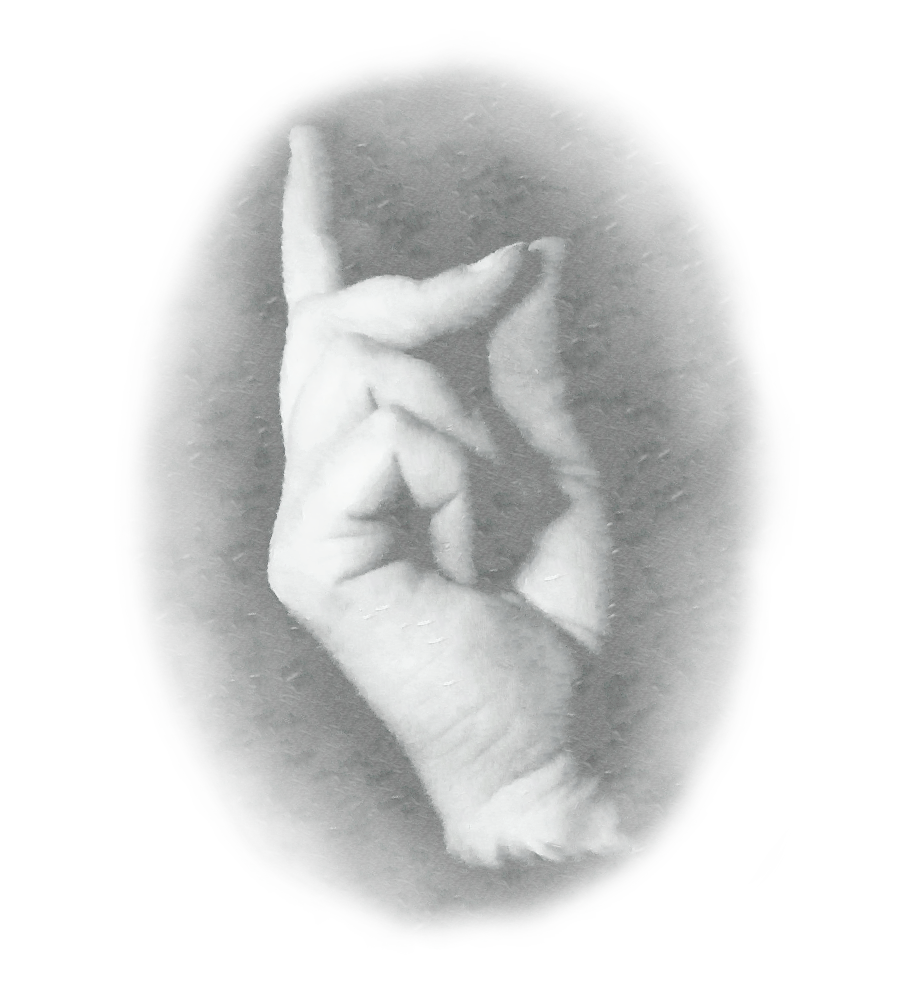
\includegraphics[scale=0.5]{bubble0.png} 
\end{vplace}

\vspace*{.5cm}
\LARGE\lumos{Eliezer\ \ \ Yudkowsky}
\normalsize


\vspace{2cm}
Find the original text at:\\
\url{http://hpmor.com} \\

\end{center}

% Begin subbook title

\cleartorecto
\begin{center}
\thispagestyle{empty}

\huge\lumos{Book\ \ }
\Huge\lumos{\hpBookNo} \vspace*{1cm}

\normalsize\lumos{\hpBookChar} \vspace*{0.2cm}

\footnotesize\lumos{and the}

\large\lumos{\hpBookTitle} \vspace*{0.5 cm}

\begin{vplace}
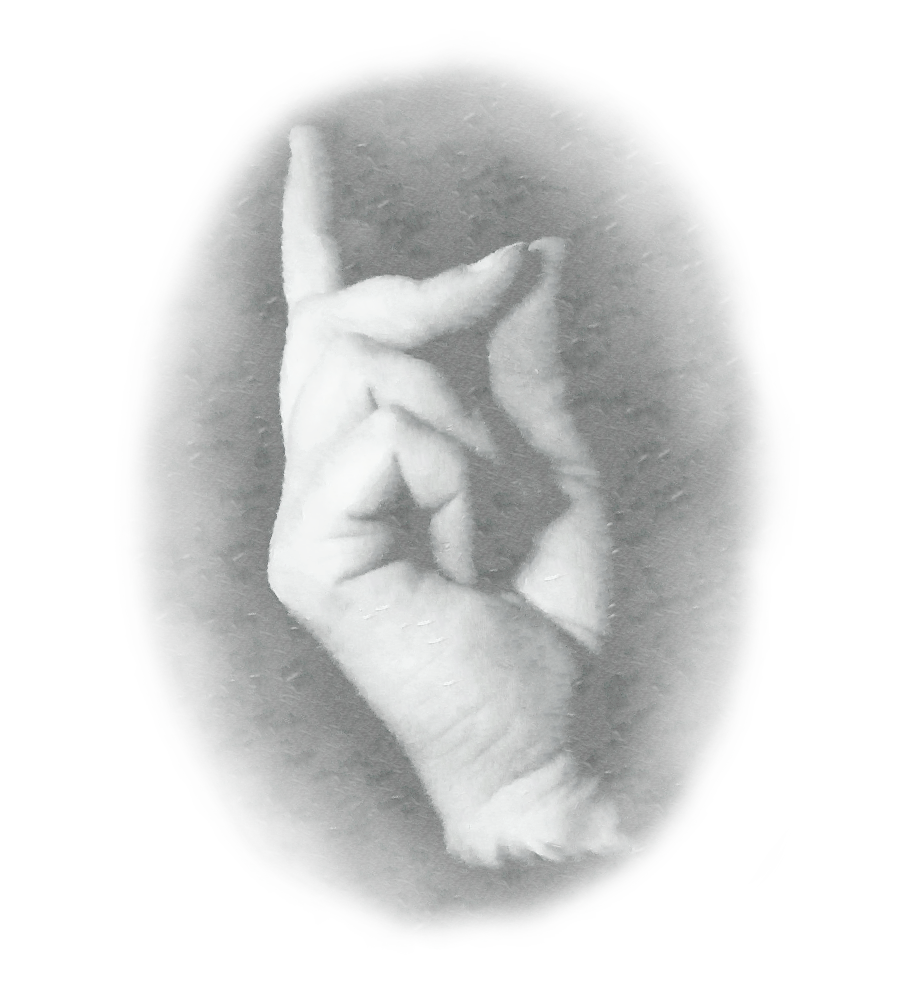
\includegraphics[scale=0.4]{bubble0.png} 
\end{vplace}

\vspace*{.5cm}
\LARGE\lumos{Eliezer\ \ \ Yudkowsky}
\normalsize

\vspace{2cm}
\mbox{\,}\\ \hpBookChapters

\end{center}

% End subbook title


\pagenumbering{gobble}
\cleartorecto
\renewcommand*{\hpmorchapbreak}{\ } % Prevent linebreaks in TOC
\renewcommand*{\printtoctitle}[1]{\centering\huge{\hp\MakeUppercase{#1}}}
\setlength{\cftbeforechapterskip}{.5\baselineskip plus 12pt minus 3pt}
\renewcommand*{\cftchapterleader}{\space—\space}
\renewcommand*{\cftchapterfillnum}[1]{%
 {\cftchapterleader}\nobreak%
 %\hbox to 1.5em{\cftchapterpagefont #1\hfil}%
 {#1}%
 \cftchapterafterpnum\par}
\setrmarg{0em}
\setlength\cftchapterindent{0pt}
\setlength\cftchapternumwidth{0pt}
\renewcommand*{\cftchapterafterpnum}{\cftparfillskip}
\renewcommand*{\cftchapterfont}{}%\small}

\renewcommand\chapternumberline[1]{\hfil\thispagestyle{empty}{\hp{\IfInteger{#1}{\NUMTONAME{#1}}{Appendix #1}}}\hfil\strut\par\nopagebreak\hfil}

\settocdepth{chapter}
\phantomsection
\label{contents}

\thispagestyle{empty}

\tableofcontents*

\clearpage
\thispagestyle{empty}
\hbox{}
\renewcommand*{\hpmorchapbreak}{\linebreak} % Restore previous functionality
\cleartorecto
}
\pagenumbering{arabic}
\setcounter{page}{1}

% Updated to an edited version of Daystar's Remix of Rationality
% https://www.fanfiction.net/s/9676374/1/Daystar-s-Remix-of-Rationality

\chapter{A Day of Very Low Probability}

\lettrine{H}{arry} James Potter-Evans-Verres was doing his best to
ignore the yelling outside his cupboard.

It was an hour before supper, and he was lying in the
cupboard under the stairs, reading a fantasy novel.
Normally, Harry enjoyed reading in companionable silence with
his father in his study, or tuning out the sound of his
mother's soap operas in the living room, but when he
wanted quiet that even his room couldn't provide, he
would go under the stairs. It was a private, cozy place,
mostly insulated from the sounds of phone conversations,
television, or outside traffic.

This particular night, however, the walls were no match for
the steadily rising voices of Michael Verres-Evans and Petunia
Evans-Verres, and soon Harry began to catch bits and
pieces of the conversation.

\emph{"{\el} just rubbish{\el} fourth time this week{\el} a silly prank,
Petunia—"}

Harry adjusted his glasses and tried to concentrate on the
book. The author was attempting to explain, through an
old wizard's limited grasp of biology and chemistry, how
the dragons in his world breathed fire. Though Harry
generally preferred science fiction, he always enjoyed
fantasy best when the writers at least tried to put some
of the magic in rational, understandable terms: it fired up
his imagination to think outside the box for what was
possible, if not terribly probable.

\emph{"{\el} not a prank, I told you{\el} have to show him, or they'll
keep{\el} more and more of them{\el}"}

\emph{"{\el} nonsense, there's no need{\el} worry about crackpots
sending him letters!"}

Unfortunately, now his imagination was preoccupied with
what kinds of letters his dad was keeping from him. Harry
closed his book, no longer able to concentrate as a familiar
bitterness flared up in him.

It wasn't that his parents mistreated him. Far from it—he'd
been sent to the best primary schools, and when that
proved insufficient he was given the best tutors an endless
pool of starving university students could provide. He'd
always been encouraged to study whatever caught his
attention, was bought all the books he wanted, was
sponsored in whatever math or science competitions he
entered. Harry knew he was exceedingly lucky, and he was
always grateful for what his parents gave him{\el} but he
would have been satisfied with half as much if it meant he
had their respect.

Of course, if asked, his parents would say they respected
him. An Oxford Professor of Biochemistry and his liberal
wife were \emph{expected} to show an enlightened view of
child-rearing that included respect. But that respect meant
something different than it would for a fellow adult, who
they would never have dreamed of talking about as if he
weren't in the house, let alone making decisions for him.

It wasn't their fault: society as a whole had such low
expectations of children. And if it was ever going to
change, it would be up to those like him to change it.

So Harry swung his legs out of the small hammock he'd
strung to the walls, turned off the lantern his father had
hung up for him, and opened the door into the hallway.

The voices immediately quieted. By the time he stepped
into the living room, his parents were sitting calmly on the
couch, watching the news on a television that stuck out
from its surroundings. Their living room was
dominated by books. Every inch of wall space was covered
by a bookcase going almost to the ceiling. Some
bookshelves were stacked to the brim with hardback
books: science, math, history, and everything else. Other
shelves had two layers of paperback science fiction, one
set right side up, the other stacked sideways in what was left
of the space above. And it still wasn't enough. Books 
overflowed onto the tables and the sofas, covered the top
of the television, and made little stacks under the windows.

"Hi, Mum, Dad. Is everything alright?"

"Hello, Harry." His mother turned to him with a warm
smile, her face still young and pretty despite her age. "Yes,
everything's fine."

"Did we disturb your reading, son?" his father said, looking
contrite. "We're sorry, our debate got a bit passionate at
the end there," Michael chuckled.

Harry and his mother exchanged knowing smiles. Professor
Verres-Evans viewed arguments as uncivilized, and so any
he participated in were automatically elevated in status to
"debate."

"It's alright. I just couldn't help overhearing,"
Harry said with mild emphasis, "and it sounded like a letter
arrived for me?"

He saw it in the quick glance they gave each other—his
mother's expectant, his father's calculating. Harry knew his
father was struggling with some mighty cognitive
dissonance. One part of him felt guilty from withholding
someone's mail from them, a grievous breach of privacy.
The other part felt entitled by societal norms that parents
were allowed to decide for their children what information
they should or shouldn't have, no matter how bright and
precocious those children might be.

"Yes," Petunia said after the silence stretched on a few
seconds. "It's the first time I've seen it, or I would have
told you sooner. Your father thinks it's just prank mail, but
he doesn't understand—"

"Well, no harm in having a look then, right?" Harry said.
He held his hand out expectantly, brow raised in an
expression of innocent patience. He wasn't quite sure what
he'd do if his father refused—trying to reason with him
rarely worked on any topic that concerned Harry's
subordinate status.

After a moment, though, his father nodded and stood up,
walking toward the trash and fishing an envelope and a
couple papers from it. "Quite right, Harry, no harm in
looking. You're a bright boy, and I know you won't get
suckered in by whatever crock they're selling."

Michael handed the letters and envelope to Harry, who
had to choke back a retort to the patronizing tone his
father had adopted now that he was giving in. Admitting
one's mistakes was for scientific journals, apparently{\el} not
for adults to do to children.

Harry chided himself on such bitter thoughts as he went
to the table. He knew this was a sore spot for him, and it
occasionally took a while for his temper to calm down. So
he forced himself to smile back at his dad, then
straightened out the first thick paper and began to
read, acutely aware of his parents' stares.
Harry's eyes scanned the letter in a few seconds, blinked,
then looked up to meet theirs.

"What."

Michael Evans-Verres smiled. "Yes, rather silly I th—"

Harry held up his hand, then looked back down at the
parchment (simple "paper" didn't suffice to describe this material)
and slowly reread the message.

\begin{writtenNote}
\letterAddress{Dear Mr.~Potter,}

We are pleased to inform you that you have been
accepted at Hogwarts School of Witchcraft and Wizardry.
Please find enclosed a list of all necessary books and
equipment.

Term begins on September 1. We await your owl by no
later than July 31.

\letterClosing[Yours sincerely,]{Minerva McGonagall, Deputy Headmistress}
\end{writtenNote}

On the second sheet he found a list that wouldn't be out
of place in a rulebook from a fantasy role-playing game.

"What is it, some kind of late summer camp?" Harry
asked as he eyed the impressive seal heading the
parchment: a lion, snake, raven and badger surrounding
an ornate \emph{H}. He smiled as he looked back at the name of
the school. \emph{Heh. "Hogwarts." What, was "Newteyes" taken?}

"No, Harry," his mother said. "It's not a summer camp. As
I was telling your father{\el}" She took a deep breath,
straightened in her seat, and avoided looking at her
husband, her gaze steady on Harry. "My sister—your mother,
Lily—was a witch. She got that same letter. I'd promised
to keep it secret, my whole family did, but now it's clear
you're meant to know, if they've come for you like they
did for her."

Harry exchanged a glance with his father, feeling a mix of
exasperation and confusion. Mum rarely spoke of his
biological parents. It wasn't taboo or anything, it just never
really came up. They'd died in a car crash when he was
one year old{\el} the same crash which had given him the
lightning shaped scar on his forehead. To hear that they
were Wiccan wasn't terribly surprising considering some of
Petunia's beliefs, but the gravity of her tone didn't match
the subject matter.

"Well that's, er, very interesting, I guess. But what does
her religion have to do with me? Who's `they?'" He didn't
particularly like the ominous sound of them "coming for
him," whoever they were. He imagined a shadowy coven
meeting in a forest and pronouncing it time to bring the
young Potter into the fold.

"It wasn't a religion. I'm saying she was an \emph{actual} witch.
She could do magic. Her husband—your father—he was a
wizard. They both went to this magic school, Hogwarts,
when they were eleven. And since you've received that letter, it
means you're a wizard too, Harry."

Michael Verres-Evans laughed, and Harry almost joined
him. Petunia Evans-Verres had always been something of
the odd-woman-out in their family. Some of the most
"spirited debates" he could remember between his parents
involved her superstitions, and he had a clear childhood
memory of her waving a crystal of some kind in careful
patterns over him when he was sick.

When he had been younger, he used to enjoy going with her to
the smoky, mysterious shops she would occasionally
frequent, with their pungent odors and exotic wares.
Thankfully his father's books had taught him how to
critically examine the beliefs sold in such places, and a few
years ago he had begun to find their air of obscure
mysticism groundless and mildly irritating.

Harry smiled down at the parchment listing the "school
supplies." Wand, spell books, potion ingredients{\el} he quickly
scanned the latter. Nope, no "hog warts" listed, though
newt eyes did indeed show up, as well as powdered hens'
teeth. He wondered how expensive that would be: he
knew there was some research being done on atavism in
chickens that resulted in them growing vestigial teeth, and
that the mutation was rather rare. Aboriginal shaman and
medicine men must have found plenty of uses for it, or
imagined them at any rate. He wondered what Hogwarts
pretended to use them for. Good dental hygiene?

And yet he didn't laugh with his father. Because{\el}

Because somewhere in him was a strange certainty that
she was right, in this most unlikely of cases.
\emph{You're a wizard too, Harry.}

"Well, maybe someday he'll be a wizard at chess," his
father said, still smiling as he turned back to the news.
"But if whoever keeps sending those letters shows up at
the door in a robe and pointy hat, I'm calling the men in
the white coats."

Petunia continued to look only at Harry, her gaze intent,
waiting.

"Mum," he said. "What do you mean by `wizard'?"

Petunia bit her lip. "I can't just tell you. You'll think I'm—"
She swallowed, and Harry felt confused. His mother had
always defended her less rational beliefs with
exasperating calmness, merely shrugging off logical arguments
and relying on some inner conviction. This sudden
nervousness, and the confusion he felt from it, made him
pay attention. "Listen. I wasn't{\el} always like this{\el}" She
gestured at herself, as though to indicate her lithe form.

"Lily did this. Because I{\el} I \emph{begged} her. For years, I
begged her. Lily had always been prettier than me, and
I'd{\el} been mean to her, because of that, and then she
got \emph{magic}, can you imagine how I felt? And I \emph{begged} her
to use some of that magic on me so that I could be
pretty too, even if I couldn't have her magic, at least I
could be pretty."

Harry watched in alarm as tears gathered in Petunia's eyes.

"And Lily would tell me no, and make up the most
ridiculous excuses, like the world would end if she were
nice to her sister, or a centaur told her not to—the most
ridiculous things, and I hated her for it. And when I had
just graduated from university, I was going out with this
boy, Vernon Dursley{\el} he was fat, and he was the only boy
who would talk to me. And he said he wanted children,
and that his first son would be named Dudley. And I
thought to myself, \emph{what kind of parent names their child
Dudley Dursley}? It was like I saw my whole future life
stretching out in front of me, and I couldn't stand it. And
I wrote to my sister and told her that if she didn't help
me I'd rather just—"

Petunia stopped. Harry felt somewhat wretched for being
responsible for her having to relate such an obviously
painful memory. A glance at his father showed his dad
similarly stricken. He'd never known that Mum had been
through such a dark period, had been so envious of her
sister{\el} he wondered how much guilt she must have felt
after his biological parents had died.

"Anyway," Petunia said, her voice small, "Lily gave in. She
warned me it was dangerous, and I said I didn't care. I
drank this potion and I was sick for weeks, but when I
got better my skin cleared up and I finally filled out and{\el}
I was beautiful. People were \emph{nice} to me," her voice broke,
"and after that I couldn't hate my sister any more,
especially when I learned what her magic brought her in
the end -"

"Darling," Michael said gently, "you got sick, you gained
some weight while resting in bed, and your skin cleared up
on its own. Or being sick made you change your diet—"

"No, it was nothing like that," Petunia said. "It was magic,
real magic. I saw it, other things—"

"Petunia," Michael said. The annoyance was creeping back
into his voice. "You \emph{know} that can't be true. Do I really
have to explain why?"

Petunia wrung her hands. She seemed to be on the verge
of tears. "My love, I know I can't win arguments with you,
but please, you have to trust me on this—"

\emph{"Dad! Mum!"}

The two of them stopped and looked at Harry. He took a
deep breath and thought about the problem. "Mum, your
parents didn't have magic, did they?"

"No," Petunia said. "Just Lily."

"Then your family also must not have believed her letter.
How did \emph{they} get convinced?"

"Ah{\el}" Petunia said. "They didn't just send a letter. They
sent a professor from Hogwarts. He—" Petunia's eyes
flicked to Michael. "He showed us some magic."

"Well, there we are then. You don't have to fight over
this," Harry said firmly. "If it's true, we can just get a
Hogwarts professor here and see the magic for ourselves,
and Dad will admit that it's true. And if not, then Mum will
admit that it's false. That's what the experimental method
is for, so that we don't have to resolve things just by
arguing." Hoping against hope that this time, just this once,
they might listen to him{\el}

"Oh, come now, Harry," Professor Verres-Evans said.
"Really, \emph{magic}? I thought you'd know better than to take
this seriously, even if you're only ten."

\emph{I. Shall. SCREAM.}

"Mum," Harry said instead, keeping his voice calm. "If you
want to win this argument with Dad, look in chapter two
of the first book of the \emph{Feynman Lectures on Physics}.
There's a quote there about how philosophers say a great
deal about what science absolutely requires, and it's all
wrong, because the only rule in science is that the final
arbiter is observation—that you just have to look at the
world and report what you see. Um{\el} off the top of my
head I can't think of where to find something about how
it's an ideal of science to settle things by experiment
instead of arguments—"

His mother looked at him and smiled. "Thank you, Harry.
But," she looked back at her husband. "I don't want to
win an argument with your father. I want my husband to
just{\el} listen to his wife who loves him, and trust her just
this once{\el}"

Harry closed his eyes briefly. \emph{Hopeless}. Both his parents
were hopeless.

Now they were getting into one of \emph{those} arguments again,
one where his mother tried to make her husband feel
guilty, and his father tried to make his wife feel stupid.

"I'm going to go to my room," Harry announced. His voice
trembled a little. "Please try not to fight too much about
this, Mum, Dad, we'll know soon enough how it comes out, right?"

"Of course, Harry," said his father, and his mother gave
him a reassuring kiss, and then they went on "debating"
while Harry climbed the stairs to his bedroom.

He shut the door behind him and tried to think, wandering
past his own bookshelves crammed with textbooks and
sci-fi to lie on his bed.

The funny thing was, he \emph{should} have agreed with Dad. No
one had ever seen any evidence of magic, and according
to Mum, there was a whole magical world out there. How
could anyone keep something like that a secret in a world
of video cameras and spy satellites? More magic? That
seemed like a rather suspicious sort of excuse.

Except that some part of Harry was utterly convinced that
what his Mum said was true. He was magic{\el} a wizard.

Was it simple ego? What child didn't want to believe they
possessed hidden, magic powers? He knew he had an
inflated sense of self-importance as others judged it. He'd
always vowed to one day justify it by proving himself
unique. Of course, he'd figured it would be somewhere in
the realm of science. He'd imagined becoming a world
renowned biologist, curing cancer and extending lifespans
indefinitely. Or going into physics to perfect cold fusion,
ending the planet's energy needs and propelling humanity
to the stars. Reasonable things. Mostly. Not magic, at any
rate.

Maybe his powers of reason had been impaired somehow.
He frowned, probing his skull with his fingers as if some
wound would present itself. He hadn't hit his head on
anything lately{\el} not that he could remember in any case.
\emph{Would} he even remember? There was a scary thought.
Harry mentally jumped through some quick mental hoops
to confirm that yes, the least complicated answer that fits all
the facts is most likely to be the true one, that all claims
require evidence and that extraordinary claims require
extraordinary evidence, that two plus two is still four.

It should have been a clean case for Mum joking, lying or
being insane, in ascending order of awfulness. If Mum had
sent the letter herself, that would explain how it arrived at
the letterbox without a stamp. A little insanity was far, far
less improbable than the universe really working like the
contents of that letter implied.

What about his mother's other views? Was he any more
susceptible to those? He considered her belief that atoms
arranged in a particular pattern identified as a "crystal"
could somehow destroy bacteria or viruses in his body
when touched to his skin{\el} specifically those bacteria or
viruses deemed "harmful," opposed to all the beneficial
ones{\el} Yes, that he could still rationally reject as a form of
wish fulfillment without any evidence to back it up. If the
person from Hogwarts came to their house and started
bending spoons, he would toss the letter in the trash and
think nothing further of it.

But that {\el} was magical... that irrational belief still stayed.
And he could think of no evidence to account for it{\el} no
moments in his life when he'd exhibited supernatural or
inexplicable powers, no hidden talent manifesting in times
of great peril or passion. Yet he still believed he had magic.

Harry rubbed his forehead, grimacing. \emph{Don't believe
everything you think}, Harry reminded himself. \emph{So where
do you come from, strange little prediction? Why do I
believe what I believe?}

Usually Harry was pretty good at answering that question,
but in this particular case, he had no \emph{clue} what his brain
was thinking. He hadn't had a belief so clearly based on
faith since he was very young. Some people, unfamiliar
with rationalism or the scientific method, seemed to think
that science took faith, since no one did every experiment
themselves, but rather relied on other scientists or
textbooks to tell them what was true or not true.

The problem with this view was that no scientist had
"faith" in textbooks, other scientists, or even the scientific
method. They had \emph{confidence} in them. Somewhere,
someone was able to do the experiments, verified the
results through repeated tests, and then subjected their
findings to peer review so others could repeat the
experiments. And if he wanted, Harry could take the time
and effort to learn the information and repeat the
experiment himself. Belief in science relied on the \emph{external},
not the internal, and thus could be shown to others,
taught and learned. He no more had faith in science than
he had faith that Dad's car would start tomorrow: he had
confidence based on experimentation and observation.

This new belief, however, was not based on external
factors. He couldn't describe it to anyone in a way that
would make sense. He couldn't demonstrate the belief and
have it peer reviewed. It just was.

Harry mentally shrugged. A button calls to be pushed, a
handle yearns to be turned, and the thing to do with a
testable hypothesis is to go and test it.

He went to his desk, shoved some of the books to the
side, took a piece of lined paper from a drawer, and began writing.

\begin{writtenNote}
\letterAddress{Dear Deputy Headmistress}
\end{writtenNote}

Harry paused, reflecting; then he discarded the paper for another, tapping another
millimeter of graphite from his mechanical pencil. This called for careful
calligraphy.

\begin{writtenNote}
\letterAddress{Dear Deputy Headmistress Minerva McGonagall,}

\letterAddress{Or Whomsoever It May Concern:}

I recently received your letter of acceptance to Hogwarts, addressed to
Mr.~H.~Potter. You may not be aware that my genetic parents, James Potter and
Lily Potter (formerly Lily Evans) are dead. I was adopted by Lily's sister,
Petunia Evans-Verres, and her husband, Michael Verres-Evans.

I am extremely interested in attending Hogwarts, conditional on such a
place actually existing. Only my mother Petunia says she knows about magic, and
she can't use it herself. My father is highly skeptical. I myself am uncertain.
I also don't know where to obtain any of the books or equipment listed in your
acceptance letter.

Mother mentioned that you sent a Hogwarts representative to Lily Potter
(then Lily Evans) in order to demonstrate to her family that magic was real,
and, I presume, help Lily obtain her school materials. If you could do this for
my own family it would be extremely helpful.

\letterClosing[Sincerely,]{Harry James Potter-Evans-Verres.}
\end{writtenNote}

Harry added their current address, then folded up the letter and put it in an
envelope, which he addressed to Hogwarts. Further consideration led him to
obtain a candle and drip wax onto the flap of the envelope, into which, using a
penknife's tip, he impressed the initials H.J.P.E.V. If he was going to descend
into this madness, he was going to do it with style.

Then he opened his door and went back downstairs. His
father was sitting in the living-room and reading a book of
higher mathematics to show how smart he was, and his mother
was in the kitchen preparing one of his father's favorite
meals to show how loving she was. It didn't look like they
were talking to one another at all. As scary as arguments
could be, \emph{not arguing} was somehow much worse.

"Mum," Harry said into the unnerving silence, "I'm going to
test the hypothesis. According to your theory, how do I
send a letter to Hogwarts?"

His mother turned from the sink to look at him uncertainly.
"I don't know{\el} I think you have to own a magic owl."

That should have sounded highly suspicious, \emph{oh, so there's
no way to test your theory then}, but the peculiar
certainty in Harry seemed willing to stick its neck out even further.

"Well, the letter got here somehow," Harry said, "so I'll
just wave it around outside and call `letter for Hogwarts!'
and see if an owl picks it up. Dad, do you want to come and watch?"

His father shook his head minutely and kept on reading.
\emph{Of course}, Harry thought to himself. Magic was a
disgraceful thing that only stupid people believed in; if his
father went so far as to \emph{test} the hypothesis, or even
\emph{watch} it being tested, that would feel like \emph{associating}
himself with that{\el}

Only as Harry stumped out the back door into the garden
did it occur to him that if an owl \emph{did} come down and
snatch the letter, he was going to have some trouble
telling Dad about it.

\emph{But—well—that can't \emph{really} happen, can it? No matter
what my brain seems to believe. If an owl really comes
down and grabs this envelope, I'm going to have worries
a lot more important than what Dad thinks.}

Harry took a deep breath and raised the envelope into the air.

He swallowed.

Calling out "\emph{Letter for Hogwarts!}" while holding an envelope
high in the air in the middle of your own back garden
was{\el} actually pretty embarrassing, now that he thought
about it.

\emph{No. I'm better than this. I will use the scientific method
even if the result makes me feel stupid.}

"Letter—" Harry said, but it actually came out as more of a
whispered croak.

Harry steeled his will and shouted into the empty sky,
"\emph{Letter for Hogwarts! Can I get an owl?}"

"Harry?" asked a bemused woman's voice from nearby.

Harry yanked his hand down as if it had caught fire,
hiding the envelope behind his back. His whole face was hot with shame.

An old woman's face peered out from over the
neighboring fence, her grizzled grey hair escaping from her
hairnet. Mrs.~Figg, the occasional babysitter. "What are you
doing, Harry?"

"Nothing," Harry said in a strangled voice. "Hi, Mrs.~Figg.
I'm just{\el} testing a really silly theory—"

"Did you get your acceptance letter from Hogwarts?"

Harry froze.

"Yes," Harry's lips said a little while later. "I got a letter
from Hogwarts. They say they want my owl by July 31, but—"

"But you don't \emph{have} an owl. Poor dear! I can't imagine
\emph{what} someone must have been thinking, sending you just
the standard letter."

A wrinkled arm stretched out over the fence and opened
an expectant hand. Hardly thinking himself at this point,
Harry gave over his envelope.

"Just leave it to me, dear," said Mrs.~Figg, "and in a jiffy
or two I'll have someone over."

And her face disappeared from over the fence.

There was a long silence in the garden.

Then Harry's voice said, calmly and quietly, "What."

\chapter{Everything I Believe Is False}

\lettrine{O}{ddly} enough, it might have been easier explaining to his
dad that an owl had grabbed the letter after all.

"What? \emph{Mrs.~Figg?}" Professor Verres-Evans's shock was
spectacular. Harry empathized completely. He sat at the
table between the living room and kitchen, somewhat in a daze.

"Did she say what time they would be coming?" Petunia
asked. She checked the pot roast and ran her hands over
her hair, as if expecting someone to ring the doorbell at any minute.

"We've known Mrs.~Figg for ten years," Harry's dad said.
"She's a perfectly reasonable woman. Why on earth would
she—"

"No, Mum, she just said they'd be here in a `jiffy or two.'
I don't know how far they're coming from, but it's probably not
going to be{\el}" Harry trailed off as he realized that, given
the hypothesis being tested, it might well be before the pot
roast was done. He tried to remind himself how silly that was—
teleportation would break so many laws of physics there
might as well not be any—but ever since he'd heard Mrs.~Figg
speak the name "Hogwarts," his brain
didn't seem to be working properly. A part of his mind
took note of his dad's comment about knowing Mrs.~Figg
for ten years. Had she moved here the year Harry had
been adopted? That seemed significant, if he could only
wrestle his mind into considering how.

"Maybe \emph{she} sent the letters," Dad said. He began to to
pace the limited floorspace of the living room, stepping
around books with the unconscious ease of memory. "Or perhaps
she's part of the same cult your sister was in—"

"Well, we'd better set an extra place just in case." Mum put a
stack of plates in front of Harry, and he set the table for
four, placing each fork and knife with an inordinate amount
of attention. Dad's theories made sense, of course, more
sense than his did, but his strange certainty continued to
color all his thoughts as he set out the cups.

A knock at the door froze them all in place.

Professor Verres-Evans was the first to thaw. He straightened, squared his
shoulders, and walked to the front door, dignity fully
reinforced by his casual tweed outfit.

Mum wiped her hands on a towel and followed. Harry
rushed after them, wondering if it would be Mrs.~Figg yet
knowing somehow that it wasn't. Dad peered through the
peephole and recoiled as if stung. Harry's anticipation redoubled.

"Yes, who's there?" Professor Verres-Evans's voice did not tremble.

"Professor Minerva McGonagall," said a formal, Scottish
voice, and Michael twitched. Harry wondered why, until his
dad opened the door.

Professor McGonagall was an older woman, perhaps in her
sixties, with greying hair in a severe bun and square
spectacles perched on her nose. She looked every inch
the professor she claimed to be, but for two things: she
wore a black robe of some rich fabric, and her hat was
decidedly pointy.

Harry grinned. His father's mental image of "professor" had
just been severely abused.

"Come in, please," Petunia said with a smile. "Supper's
almost ready, if you're hungry."

"I ate, thank you." Professor McGonagall said as she walked
inside. Harry and his parents stepped back to let her through.

"I'm Petunia Evans-Verres, so nice to meet you{\el}" The two
walked down the hall, leaving Harry and his dad by the
door. Harry closed it, then exchanged a look with his father.

"What do you reckon?" Harry whispered. "Time to call the white coats?"

Dad snorted and clapped him on the shoulder with a grin.
"Come on, let's get this foolishness done with." They
followed the women into the living room.

"Got an experiment in mind?" Harry asked. He was still
feeling off balance. That strange certainty was stronger
now, as if all this were a formality, and he had already
accepted that the woman in their house was a witch,
without quite being able to grasp what that would mean in
a practical sense.

"I can't imagine anything I would come up with that she
wouldn't make an excuse for," his father said, still keeping
his voice low. Harry nodded in response, and then he decided to be forthright
with their guest, who stood expectantly in the living room.
She eyed the multitude of books with what looked to be
an admiring air, which Harry found reassuring.

"Good evening, Professor McGonagall. As I'm sure you're
aware—" Harry stopped. He actually wasn't sure \emph{what} she
was aware of. Had she received his letter? What had Mrs.~Figg done,
read it to her over the phone? Perhaps she
had stopped next door to retrieve it before coming here{\el}
Harry stifled his questions and began again. "I'm Harry
Potter-Evans-Verres. We were surprised by your letter, and
have some doubts about its validity. Mum says she's seen
magic before, but neither Dad nor myself have. If you
could demonstrate the quality of your magic to us, that
would be a good first step."

Professor McGonagall was watching Harry with an amused
expression as he spoke. "Of course. I would be happy to."
She pulled a thin wooden stick out of her sleeve with
practiced grace, and Harry blinked. He hadn't seen the
shape of it against the material, and it should have fallen
out if it wasn't held there somehow. "Is there something
specific that would persuade you?"

Still preoccupied with her sleight of hand, it took Harry a
second to realize she was holding a \emph{magic wand}, and he
said the first thing that popped into his head: "Can you
shoot fire out of that?"

"Harry!" Mum said with some alarm, and Professor
McGonagall's lips twitched in a brief smile.

"I could, but I think that would be dangerous." She
glanced pointedly at their surroundings. "How about
something less destructive?"

"Of course," Harry said, cheeks red. "Er{\el} did you fly
here? I didn't hear a car, and unless you live nearby I
can't imagine how else you got here so quickly. If you
could just{\el} hover a bit? That might help. Wait, on second
thought, levitate Dad."

Professor Verres-Evans gave Harry an approving nod, and
stepped forward to face their guest with his arms crossed.
Professor McGonagall lifted her wand, and Harry realized
his mistake. "Wait!" he said. She lowered her wand, raising
an eyebrow. "I want to make sure we do this right." He
thought about it for a second while everyone watched him.

"Now, just to be clear," Harry said to his father. "If Professor
McGonagall does levitate you, when you know you haven't
been attached to any wires, that's going to be sufficient
evidence. You're not going to turn around and say that it's
a magician's trick. That wouldn't be fair play. If you feel
that way, you should say so now, and we can ask her to
do something else instead."

Dad nodded, smiling good-naturedly. "Agreed."

"And you, Mum, your theory says that the professor
should be able to do this, and if that doesn't happen,
you'll admit you're mistaken. Nothing about how magic
doesn't work when people are skeptical of it, or anything
like that."

Mum glanced at Professor McGonagall's wand and nodded.

"Is that sufficient, Mr. Potter?" Professor McGonagall said.
"Shall I go ahead and demonstrate?"

"Sufficient? Probably not, but it should do for now," Harry
said. Once he saw her methodology he could better decide
how to isolate her actions and their relation to the result{\el}
assuming there was a result. Did he really expect his
father to start floating? "Proceed, please."

"Is there anything you'd like me to do?" Professor
Verres-Evans said, still smiling. "Think light thoughts,
perhaps?"

"No need, thank you," Professor McGonagall replied, and
then, "\emph{Wingardium Leviosa}."

There was a silent pause that Harry knew he would
always remember{\el} the moment when his world utterly
changed. Everything was still, as if suspended in crystal:
he and his mother staring in shock, the witch holding her
wand pointed up at his father, who hung a respectable
three feet off the ground in complete defiance of gravity.

Harry looked up at his father.

"Huh."

His father looked down at him.

And then Professor Verres-Evans looked back at Professor
McGonagall and said, in a voice Harry had never heard him
use, "All right, you can put me down now, thank you."

Harry's father was lowered carefully to the ground, and the
moment was ended. The universe continued on just as it had before.

Harry ruffled a hand through his dark hair. Maybe it was
just that strange part of him which had \emph{already} been
convinced, but{\el} "That's a bit of an anticlimax," Harry said.
"You'd think there would be some kind of more dramatic
mental event associated with updating on an observation of
infinitesimal probability—" Harry stopped himself. Mum and
the witch were looking at him oddly. Dad slowly sat down,
not even bothering to move the book from the chair as
he stared at the piece of wood in Professor McGonagall's
hand. "I mean, with finding out that everything I believe is false."

Seriously, it should have been more dramatic. His brain
ought to have been flushing its entire current stock of
hypotheses about the universe, none of which allowed this
to happen. But instead it just seemed to be going, \emph{All
right, I saw the Hogwarts Professor wave her wand and
make Dad rise into the air, now what?}

The witch was smiling benevolently upon them, looking
quite amused. "Would you like a further demonstration, Mr.~Potter?"

"You don't have to," Harry said. "We've performed a definitive
experiment. That wasn't some trick with mirrors, it wasn't
hypnotic suggestion, he actually lifted off the ground, we all
saw it{\el} but{\el}" Harry hesitated. He couldn't help himself.
Actually, under the circumstances, he \emph{shouldn't} be helping
himself. It was right and proper to be curious. "What else
\emph{can} you do?"

"Besides shoot fire, you mean?"

Dad looked as alarmed as Mum had a moment ago.

"Yes, besides that." Though Harry actually would love to
see it. He was starting to get excited. Would he really be
able to fly? Conjure fire at will? How? Did he accelerate
the atoms in the air until they combusted? \emph{Maybe I use
my body heat to—}

Professor McGonagall turned into a cat.

Harry scrambled back unthinkingly, backpedaling so fast that he tripped over a
stray stack of books and landed hard on his bottom. His
hands came down to catch himself without quite reaching properly, and there was
a warning twinge in his shoulder as the weight came down unbraced.

At once the small tabby cat morphed back up into a robed woman. "I'm sorry,
Mr.~Potter," said the witch, sounding sincere, though the corners of her lips
were twitching upwards. "I should have warned you."

Harry was breathing in short gasps. His voice came out choked.
"\emph{You can't DO that!}"

"It's only a Transfiguration," said Professor McGonagall. "An Animagus
transformation, to be exact."

"You turned into a cat! A \emph{SMALL} cat! You violated Conservation of
Energy! That's not just an arbitrary rule, it's implied by the form of the
quantum Hamiltonian! Rejecting it destroys unitarity
and then you get faster-than-light signaling!
And cats are \emph{COMPLICATED!} A human mind can't just visualize
a whole cat's anatomy and, and all the cat biochemistry, and what about the
\emph{neurology?} How can you go on \emph{thinking} using a cat-sized brain?"

Professor McGonagall's lips were twitching harder now. "Magic."

"Magic \emph{isn't enough} to do that! You'd have to be a god!"

Professor McGonagall blinked. "That's the first time I've ever been called
\emph{that}."

A blur was coming over Harry's vision, as his brain started to comprehend what
had just broken. The whole idea of a unified universe with mathematically
regular laws, that was what had been flushed down the toilet; the whole notion
of \emph{physics}. Three thousand years of resolving big complicated things
into smaller pieces, discovering that the music of the planets was the same
tune as a falling apple, finding that the true laws were perfectly universal
and had no exceptions anywhere and took the form of simple mathematics governing the
smallest parts, \emph{not to mention} that the mind was the brain and the brain
was made of neurons, a brain was what a person \emph{was}—

And then a woman turned into a cat, so much for all that.

A hundred questions fought for priority over Harry's lips, and the winner poured
out: "And, and what kind of incantation is \emph{Wingardium Leviosa}? Who
invents the words to these spells, nursery schoolers?"

"That will do, Mr.~Potter," Professor McGonagall said crisply, though her eyes
shone with suppressed amusement. "If you wish to learn about magic, I suggest
that we finalize the paperwork so that you can go to Hogwarts."

"Right," Harry said, somewhat dazed. Paperwork. Some things
never changed, it seemed, even in a world of magic.
He pulled his thoughts together. The March
of Reason would just have to start over, that was all.
They still had the experimental method, and that was the important thing.

"Are you alright, darling?" Mum said, putting a hand on her
husband's shoulder.

Professor Verres-Evans did look rather pale. He patted her
hand. "I{\el} I think so, dear, thank you." He then brought
her hand to his lips in a rare show of public affection.
"And{\el} I'm sorry."

Petunia smiled and squeezed his hand. "That's alright. I
was just as doubtful with Lily, and I didn't have half as
many good reasons to be as you."

Dad smiled at her, then looked at Harry. "I apologize to
you too, son. You were right. `The final arbiter is
observation,' indeed. I don't know if I can quite take all
this in properly, but{\el}"

Harry had choked up a bit, and now he smiled back at his
parents. "I had some help, or I would probably have been
just as doubtful. Maybe it's a wizard thing. I'll explain
another time." He turned to Professor McGonagall, who he
now remembered was also the Deputy Headmistress to
Hogwarts. A real school for wizards and witches. He
couldn't begin to imagine what it would be like, with
professors like this. "I'm ready. How do I get to Hogwarts?"

A choked laugh escaped Professor McGonagall, as if extracted from her by
tweezers. "I won't be whisking you away by
magic, if that's what you're expecting. As the letter said,
term starts September 1. I will come again and explain
how transportation will occur, as well as help you obtain
your school supplies."

"Hold on a moment, Harry," his father said. "Remember why you haven't been
going to school up until now? What about your condition?"

Professor McGonagall spun to face Michael. "His condition? What's this?"

"I don't sleep right," Harry said. He waved his hands helplessly. "My sleep
cycle is twenty-six hours long, I always go to sleep two hours later, every
day. I can't fall asleep any earlier than that, and then the next day I go to
sleep two hours later than \emph{that}. 10\PM, 12\AM, 2\AM, 4\AM, until it goes
around the clock. Even if I try to wake up early, it makes no difference and
I'm a wreck that whole day. That's why I haven't been going to a normal school
up until now."

"One of the reasons," said his mother. Harry winced. He
didn't want his potential future teacher and Deputy
Headmistress to have a biased opinion of him.

\emph{Even if it might be a bit deserved?} asked his Inner Critic.

\emph{It could be important for the teachers to know,}
commented his utilitarian side. \emph{Remember when our science project—}

\emph{Shut up or they might not teach us magic!} said his Id,
and the other parts of Harry promptly fell into agreed silence.

McGonagall gave a long \emph{hmmmmm.} "I can't recall hearing about such a
condition before{\el}" she said slowly. "I'll check with Madam Pomfrey to
see if she knows any remedies." Then her face brightened. "No, I'm sure this
won't be a problem—I'll find a solution in time. Now," and her gaze sharpened
again, "what are these \emph{other} reasons?"

Harry sent his parents a glare, then straightened his
shoulders. "I," he said with deliberate gravity, "am a
conscientious objector to child conscription. On grounds that
I should not have to suffer for a disintegrating school
system's failure to provide teachers or study materials of
even minimally adequate quality."

Both of Harry's parents burst out laughing.
"Oh," said Harry's father, eyes bright, "is \emph{that} why you
bit a math teacher in third year?"

"\emph{She didn't know what a logarithm was!}"

"Of course," seconded Mum. "And biting her was a very mature response."

Dad nodded. "A well-considered policy to address the
failings of a disintegrating school system."

"I was \emph{seven years old!} How long are you going to keep on bringing that
up?"

"I know," said his mother sympathetically, "you bite \emph{one} teacher
and they never let you forget it, do they?"

Harry turned to Professor McGonagall as his father
chuckled. "Are you sure you can't just whisk me away now?"

"Quite sure." Professor McGonagall's restrained smile
threatened to burst into a grin at any moment. "And there
is to be no biting of teachers at Hogwarts, is that quite
clear, Mr. Potter?"

Harry scowled at her. "Fine, I won't bite anyone who
doesn't bite me first."

"Better not ask him to build a volcano either," Dad
suggested, as his mother began howling with laughter.
"Not unless this school of yours is magically fireproof."

"\emph{Dad!}" Harry yelled, cheeks burning.

"Well{\el}" Professor McGonagall said. "I think, under the
circumstances, that I should avoid taking you to purchase
your study materials until a day or two before school begins."

"What? \emph{Why?} The other children already know magic, don't
they? I have to start catching up right away! I promise
not to burn down the school!" It occurred to him exactly a
second after saying it out loud that his having to say it
was not particularly encouraging.

"Rest assured, Mr.~Potter," replied Professor McGonagall,
"Everyone at Hogwarts will begin with the basics, and the
school is quite capable of teaching its students without risk
of self-destruction. On the other hand, I suspect that if I
leave you alone for two months with your schoolbooks,
even without a wand, I will return to this house only to
find a crater billowing purple smoke, a depopulated city
surrounding it, and a plague of flaming zebras terrorizing
what remains of Oxford."

Harry's mother and father nodded in perfect unison.

"\emph{Mum! Dad!}"

\chapter{Comparing Reality To Its Alternatives}

\lettrine{P}{etunia} Evans-Verres looked at Harry in the rear-view
mirror of the car as if she could easily guess his thoughts,
and seemed troubled by them. He'd spent the past few
weeks in a mild frenzy, first interrogating her for what little
direct experience she had about magic ("No, Mum, tell me
what you've \emph{seen}, not what you've guessed or read
about.") then doing independent research, which had
quickly proven fruitless. Any books on magic he found
involved complicated rituals to bring about some minor,
vague misfortune, or wishing yourself riches and happiness
through "positive attraction," or some other such
unfalsifiable feel-good fluff. Nothing \emph{remotely} close to lifting
a man off the ground with a couple words and the wave
of a stick, let alone turning into a cat, and no mention of
a "Hogwarts" anywhere.

Clearly all the \emph{real} magic was kept out of bookstores or
libraries by some organized effort, a notion he found both
troubling and thrilling. On the one hand, he was about to
be part of a massive, worldwide conspiracy the likes of
which he'd only read about in fiction. On the other hand,
the reality of a group of people capable of secretly
enforcing such a conspiracy was mildly terrifying. He
wondered how omnipotent they really were, and whether
non-magic authorities were involved in the cover-up.

The day before yesterday, another message had
arrived at their house. Professor McGonagall had supplied
them with a time and an address where Harry could meet
her to obtain his school supplies. So this morning, Harry's
mother had driven him to London, uncharacteristically quiet
and nervous. Harry assumed she was worried he would
make a bad impression, but he was determined not to get
into any trouble that might jeopardize his acceptance into
the magical world. If the past few weeks had confirmed
anything about his nature to himself, it was that he
couldn't stand being aware of a mystery and not having
the means to solve it. Just imagining going on with his life
without learning more about magic{\el} any scientific field he
went into would drive him mad as he considered the true
nature of reality that he'd caught a glimpse of.

Once they arrived at the appropriate address, Harry's
mother parked beside a row of shops. Harry stepped out
of the car and looked around, and his mother rolled down
her window.

"Well," Petunia said after a pause, looking up and down
the sidewalk. "I don't see Professor McGonagall{\el} though
we are a bit early. Where do you suppose the place is?
`The Leaky Cauldron,' wasn't it?"

Harry turned in a slow circle, scanning the shops along the
street. Nothing looked like a place that would sell magic
wands, even as a joke. There was a fashionable clothing
store, a hair boutique, an ice cream parlor, some fast food
restaurants, a book shop (which he quickly jogged into,
looked around a bit, then left), a pub—"There," he said,
pointing to The Leaky Cauldron, a quaint brick building
tucked between the book shop and a record store. "Maybe
she's already inside."

"Hm?" Harry's mother looked vaguely in the direction he'd
pointed. "Did you say you saw her?"

Harry began to point again, then stopped and looked at
his Mum, then back at the pub. She was looking right at
it. "What do you see between that bookshop and the
record store?"

"What do you mean, dear? In the alley?"

\emph{Alley?} From Harry's perspective, the walls of The Leaky
Cauldron were pressed up against its neighbors. "You don't
see the pub right there?" he asked, pointing straight at it
again.

"No," Petunia said. "You mean to tell me there is one?"

Harry felt an electric thrill go up his spine and simply
couldn't help himself. He approached a nearby couple.
"Excuse me. I'm afraid I brought
the wrong prescription with me this morning and can't
quite make out the store signs. Could you read them to
me please, from right to left?" He gestured.

The man gave him a curious look, but the woman began
listing names. Harry watched her eyes as she named the
book shop, then the record store, without mentioning the
Leaky Cauldron. It looked as though her gaze simply
passed over where it was without registering it.

"Thank you." He returned to his mother, shifting his weight
from foot to foot with nervous energy as he stood beside
the car and examined the pub. "It's not just you. They
couldn't see it either." Here it was. Proof, however subtle,
that he wasn't like other people. The now-familiar sense of
disorientation came over him, and his mind raced with
possibilities for how the cloaking worked. Harry wondered
what would happen if he threw a rock out of the pub's
window. Would the glass suddenly become visible to the
people on the street? It was all he could do to not rush
to the pub and begin experimenting with his mother's
perception.

If wizard folk could do things like \emph{this}, it was no wonder
Harry couldn't find any books about them. He wondered
now if a massive conspiracy was really needed to hide
records of the magical world. What if non-magic folk
couldn't even see the books? What else had he seen in
his life without realizing no one else could? Maybe some
other safety mechanism was in place, like he needed to
know the name of the pub as well—

"Good morning, Mr.~Potter."

Harry spun around to see Professor McGonagall, who
seemed utterly unconcerned with the odd
looks she was getting from passersby.

"Good morning, Professor," Harry said. "Why can't Mum
see The Leaky Cauldron?"

"It's enchanted against Muggle notice." Professor McGonagall
turned to his mother. "Good morning, Mrs.~Evans-Verres.
I'm sorry to have kept you waiting."

"Not at all, we'd just arrived." Petunia looked back at
Harry, with the same nervous air she'd had all day.

"Well, I'll be back this evening to pick you up. Be good, Harry."

She kissed him goodbye and drove away. Harry watched his mother
go, then turned to Professor McGonagall. "What's a `Muggle?'"

Professor McGonagall's lips twitched. "It's good to see you
again too, Mr.~Potter. Muggles are what we call those
without a drop of magic in them. Shall we?"

Harry followed her toward the pub. "Okay, so Dad's a
Muggle, but Mum too? Her sister was a witch, doesn't that
mean she had some magic in her family?"

"Oh, no, if her parents were both Muggles then she's
a Muggle as well," Professor McGonagall explained in her prim,
Scottish voice. "What you're thinking of is what we call a
Squib. Though children of a witch and wizard, they cannot
perform magic themselves, but they can perceive
many magical things and use enchanted items."

Harry was trying to filter this information through his
understanding of genetics, but he was distracted partway as
they entered The Leaky Cauldron. He whipped his head
around to see if anything of note happened as they did,
but he couldn't detect any invisibility field descending on him,
and no one in the street seemed to notice two people
suddenly disappear.

The inside of the pub was somewhat dark and shabby, with
wooden tables scattered about the shadows and a grubby
bar that dominated the far wall. About a dozen people
were inside, most dressed in variously colored robes.

"Good morning, Professor McGonagall," said the barman
with a smile.

"Good morning, Tom."

"Is there anything I could get for—Good Lord." The barman
peered at Harry, gaze drawn to his forehead. "is this—can this be—?"

Harry leaned towards the bar of the Leaky Cauldron as best he could, though it
came up to somewhere around the tips of his eyebrows. A question like
\emph{that} deserved his very best.

"Am I—could I be—maybe—you never know—if I'm \emph{not}—but then the
question is—\emph{who?}"

"Bless my soul," whispered the old barman. "Harry Potter{\el} what an
honor."

Harry blinked, then rallied. "Well, yes, you're quite perceptive; most people
don't realize that so quickly—"

"That's enough," Professor McGonagall said. Her hand tightened on Harry's
shoulder. "Don't pester the boy, Tom, he's new to all this."

"But it is him?" quavered an old woman. "It's Harry Potter?" With a scraping
sound, she got up from her chair.

"Doris—" McGonagall said warningly. The glare she shot around the room
was enough to stop most others from doing
more than muttering among themselves and staring;
some paused halfway out of their seats.

"I only want to shake his hand," the woman whispered. She bent low and stuck
out a wrinkled palm, which Harry, feeling confused and more uncomfortable than
he ever had in his life, carefully shook. Tears fell from the woman's eyes onto
their clasped hands. "My grandson was an Auror," she whispered to him. "Died in
seventy-nine. Thank you, Harry Potter. Thank heavens for you."

"You're welcome," Harry said automatically, and then he turned his head and
shot Professor McGonagall a frightened, pleading look.

Others began to approach them again, and Professor
McGonagall slammed her foot down. It made a noise that
gave Harry a new referent for the phrase "Crack of
Doom", and the other bar patrons once again froze in
place just as the general rush was about to start.

"We're in a hurry," Professor McGonagall stated calmly.

They left the bar without any trouble and entered the courtyard
behind it, which was surrounded on all sides by high brick walls.

"Professor?" Harry said, meaning to ask what was going on, but oddly
finding himself asking an entirely different question instead.
"Who was that pale man, by the corner? The man with
the twitching eye, slumped in his seat?"

"Hm?" said Professor McGonagall, sounding a bit surprised; perhaps she hadn't
expected that question either. "That was Professor Quirinus Quirrell. He'll be
teaching Defense Against the Dark Arts this year at Hogwarts."

"I had the strangest feeling that I knew him{\el}" Harry rubbed his
forehead. "And that I shouldn't ought to shake his hand." Like meeting someone
who had been a friend, once, before something went drastically wrong{\el}
that wasn't really it at all, but Harry couldn't find words. "And what
\emph{was}{\el} all of that?"

Professor McGonagall was giving him an odd glance. "Mr.~Potter{\el} do you
know{\el} how \emph{much} have you been told{\el} about how your parents
died?"

Harry returned a steady look. "My parents are alive and
well, thank you. They've told me that my \emph{genetic} parents
were killed in a car accident when I was one year old."

"An admirable loyalty," said Professor McGonagall. Her voice went low. "Though
it hurts a little to hear you say it like that. Lily and James were friends of
mine."

Harry looked away, suddenly ashamed. "I'm sorry," he said in a small voice.
"But I \emph{have} a Mum and Dad. And I know that I'd just make myself unhappy
by comparing that reality to{\el} something perfect that I built up in my
imagination."

"That is amazingly wise of you," Professor McGonagall said quietly. "But your
\emph{genetic} parents died very well indeed, protecting you."

\emph{Protecting me?}

Something strange clutched at Harry's heart. "So it{\el}
wasn't a car crash? What \emph{did} happen?"

Professor McGonagall sighed. Her wand tapped Harry's forehead, and his vision
blurred for a moment. "Something of a disguise," she said, "so that this
doesn't happen again, not until you're ready." Then her wand licked out again,
and tapped three times on a brick in the wall{\el}

{\el} which hollowed into a hole that dilated and expanded and
shivered into a huge archway, revealing a cobbled street full of
odd shops advertising everything from actual \emph{cauldrons} to
\emph{dragon liver.}

Harry didn't blink. It wasn't like anyone was turning into a cat.

"Welcome, Mr.~Potter, to Diagon Alley."

And they walked forwards, together, into the wizarding world.

Here, Harry was sure, was the true testament to the
effectiveness of magical secrecy. A whole long, winding
street of London City completely unknown by its
inhabitants. Only powerful magic or political agreements of
the highest order could keep airplanes or satellites from
taking note of such a place. Here were merchants hawking
Bounce Boots ("Made with real Flubber!"). There were
goggles that would turn anything you looked at green, and
a lineup of comfy armchairs with ejection seats for
emergencies. Some of the buildings were merely a story
or two high, while others had multiple floors and were
oddly structured, as though relying on magic to keep them upright.

Harry's head kept rotating as if trying to wind itself off his
neck. It was like walking through the magical items section of an
\emph{Advanced Dungeons and Dragons} rulebook (he enjoyed
reading those, even though he had no one
to play the games with). Harry desperately didn't want to miss a
single item for sale, in case it was one of the three you needed to complete
the cycle of infinite \emph{wish} spells.

Then Harry spotted something that made him unthinkingly
veer off from the Deputy Headmistress.
He was heading straight into the shop, a front of blue bricks
with bronze-metal trim, when Professor McGonagall's voice
brought him back to reality.

"Mr.~Potter?" she said.

Harry blinked, then realized what he'd just done. "I'm sorry! I forgot for a
moment that I was with you instead of my family." Harry gestured at the shop
window, which displayed fiery letters that shone piercingly bright and yet
remote, spelling out \emph{Bigbam's Brilliant Books}. "When you walk past a
bookshop you haven't visited before, you have to go in and look around. That's
the family rule."

"That is the most Ravenclaw thing I have ever heard."

"What?"

"Nothing. Mr.~Potter, our first step is to visit Gringotts, the bank of the
wizarding world. Your \emph{genetic} family vault is there, with the
inheritance your \emph{genetic} parents left you, and you'll need money for
school supplies." She sighed. "And, I suppose, a certain amount of spending
money for books could be excused as well. Though you might want to hold off for
a time. Hogwarts has quite a large library on magical subjects. And the tower
in which I strongly suspect you will be living has a more broad-ranging
library of its own. Any book you bought now would probably be a duplicate."

Harry nodded, and they walked on.

"Don't get me wrong, it's a \emph{great} distraction," Harry said as his head
kept swiveling, "probably the best distraction anyone has ever tried on me,
but don't think I've forgotten about our pending discussion."

Professor McGonagall was silent for a time.
"Your parents—or your mother at any rate—may
have been very wise not to tell you."

"So you wish that I could continue in blissful ignorance? There is a certain
flaw in that plan, Professor McGonagall."

"I suppose it would be rather pointless," the witch said tightly, "when anyone
on the street could tell you the story. Very well."

And she told him of He-Who-Must-Not-Be-Named, the Dark Lord, Voldemort.

"Voldemort?" Harry whispered. It should have been funny, but it wasn't. The
name burned with a cold feeling, ruthlessness, diamond clarity, a hammer of
pure titanium descending upon an anvil of yielding flesh. A chill swept over
Harry even as he pronounced the word, and he resolved then and there to use
safer terms like You-Know-Who.

The Dark Lord had raged upon wizarding Britain like a wilding wolf, tearing and
rending at the fabric of their everyday lives. Other countries had wrung their
hands but hesitated to intervene, whether out of apathetic selfishness or
simple fear, for whichever was first among them to oppose the Dark Lord, their
peace would be the next target of his terror.

(\emph{The bystander effect,} thought Harry, thinking of Latane and Darley's
experiment, which had shown that you were more likely to get help if you had an
epileptic fit in front of one person than in front of three. \emph{Diffusion of
responsibility, everyone hoping that someone else would go first.})

The Death Eaters had followed in the Dark Lord's wake and in his vanguard,
carrion vultures to pick at wounds, or snakes to bite and weaken. The Death
Eaters were not as terrible as the Dark Lord, but they were terrible, and they
were many. And the Death Eaters wielded more than wands; there was wealth
within those masked ranks, and political power, and secrets held in blackmail,
to paralyze a society trying to protect itself.

An old and respected journalist, Yermy Wibble, called for increased taxes and
conscription. He shouted that it was absurd for the many to cower in fear of
the few. His skin, only his skin, had been found nailed to the newsroom wall
that next morning, next to the skins of his wife and two daughters. Everyone
wished for something more to be done, and no one dared take the lead to propose
it. Whoever stood out the most became the next example.

Until the names of James and Lily Potter rose to the top of that list.

And those two might have died with their wands in their hands and not regretted
their choices, for they \emph{were} heroes; but they had an infant
child, their son, Harry Potter.

Tears were coming into Harry's eyes. He wiped them away in anger or maybe
desperation, \emph{I didn't know those people, not really, they aren't my
parents} now, \emph{it would be pointless to feel so sad for them—}

When Harry was done sobbing into the witch's robes, he looked up, and felt a
little bit better to see tears in Professor McGonagall's eyes as well.

"So what happened?" Harry said, his voice trembling.

"The Dark Lord came to Godric's Hollow," Professor McGonagall said in a
whisper. "You should have been hidden, but you were betrayed. The Dark Lord
killed James, and he killed Lily, and he came in the end to you, to your cot.
He cast the Killing Curse at you, and that was where it ended. The Killing
Curse is formed of pure hate, and strikes directly at the soul, severing it
from the body. It cannot be blocked, and whomever it strikes, they die. But you
survived. You are the only person ever to survive. The Killing Curse rebounded
and struck the Dark Lord, leaving only the burnt hulk of his body and a scar
upon your forehead. That was the end of the terror, and we were free. That,
Harry Potter, is why you are often called `The Boy Who Lived,'
and why people want to see the scar on your forehead, and why they
want to shake your hand."

The storm of weeping that had washed through Harry had used up all his tears;
he would not cry again.

(And somewhere in the back of his mind was a small, small note of confusion, a
sense of something wrong about that story; and it should have been a part of
Harry's art to notice that tiny note, but he was distracted. For it is a sad
rule that whenever you are most in need of your art as a rationalist, that is
when you are most likely to forget it.)

Harry detached himself from Professor McGonagall's side. "I'll—have to think
about this," he said, trying to keep his voice under control. He stared at his
shoes. "Um. You can go ahead and call them my parents, if you want, you don't
have to say `genetic parents' or anything. I guess there's no reason I can't
have two mothers and two fathers."

There was no sound from Professor McGonagall.

And they walked together in silence, making their way through the enchanted street.

%\chapter{The Efficient Market Hypothesis}

\lettrine{H}{eaps} of gold Galleons. Stacks of silver Sickles. Piles of bronze Knuts.

\quad\quad
Harry stood there, and stared with his mouth open at the family vault. He had
so many questions he didn't know \emph{where} to start.

From just outside the door of the vault, Professor McGonagall watched him,
seeming to lean casually against the wall, but her eyes intent. Well, that made
sense. Being plopped in front of a giant heap of gold coins was a test of
character so pure it was archetypal.

"Are these coins the pure metal?" Harry said finally.

"What?" hissed the goblin Griphook, who was waiting near the door. "Are you
questioning the integrity of Gringotts, Mr.~Potter-Evans-Verres?"

"No," said Harry absently, "not at all, sorry if that came out wrong, sir. I
just have no idea at all how your financial system works. I'm asking if
Galleons in general are made of pure gold."

"Of course," said Griphook.

"And can anyone coin them, or are they issued by a monopoly that thereby
collects seigniorage?"

"What?" said Professor McGonagall.

Griphook grinned, showing sharp teeth. "Only a fool would trust any but goblin
coin!"

"In other words," Harry said, "the coins aren't supposed to be worth any more
than the metal making them up?"

Griphook stared at Harry. Professor McGonagall looked bemused.

"I mean, suppose I came in here with a ton of silver. Could I get a ton of
Sickles made from it?"

"For a fee, Mr.~Potter-Evans-Verres." The goblin watched him with glittering
eyes. "For a certain fee. Where would you find a ton of silver, I wonder?"

"I was speaking hypothetically," Harry said. \emph{For now, at any rate.}
"So{\ldots} how much would you charge in fees, as a fraction of the whole
weight?"

Griphook's eyes were intent. "I would have to consult my superiors{\ldots}"

"Give me a wild guess. I won't hold Gringotts to it."

"A twentieth part of the metal would well pay for the coining."

Harry nodded. "Thank you very much, Mr.~Griphook."

\emph{So not only is the wizarding economy almost completely decoupled from the
Muggle economy, no one here has ever heard of arbitrage.} The larger Muggle
economy had a fluctuating trading range of gold to silver, so every time the
Muggle gold-to-silver ratio got more than 5\% away from the weight of seventeen
Sickles to one Galleon, either gold or silver should have drained from the
wizarding economy until it became impossible to maintain the exchange rate.
Bring in a ton of silver, change to Sickles (and pay 5\%), change the Sickles
for Galleons, take the gold to the Muggle world, exchange it for more silver
than you started with, and repeat.

Wasn't the Muggle gold to silver ratio somewhere around fifty to one? Harry
didn't think it was seventeen, anyway. And it looked like the silver coins were
actually \emph{smaller} than the gold coins.

Then again, Harry was standing in a bank that \emph{literally} stored your
money in vaults full of gold coins guarded by dragons, where you had to go in
and take coins out of your vault whenever you wanted to spend money. The finer
points of arbitraging away market inefficiencies might well be lost on them.
He'd been tempted to make snide remarks about the crudity of their financial
system{\ldots}

\emph{But the sad thing is, their way is probably better.}

On the other hand, one competent hedge fundie could probably own the whole
wizarding world within a week. Harry filed away this notion in case he ever ran
out of money, or had a week free.

Meanwhile, the giant heaps of gold coins within the Potter vault ought to suit
his near-term requirements.

Harry stumped forward, and began picking up gold coins with one hand and
dumping them into the other.

When he had reached twenty, Professor McGonagall coughed. "I think that will be
more than enough to pay for your school supplies, Mr.~Potter."

"Hm?" Harry said, his mind elsewhere. "Hold on, I'm doing a Fermi calculation."

"A \emph{what?}" said Professor McGonagall, sounding somewhat alarmed.

"It's a mathematical thing. Named after Enrico Fermi. A way of getting rough
numbers quickly in your head{\ldots}"

Twenty gold Galleons weighed a tenth of a kilogram, maybe? And gold was, what,
ten thousand British pounds a kilogram? So a Galleon would be worth about fifty
pounds{\ldots} The mounds of gold coins looked to be about sixty coins high and
twenty coins wide in either dimension of the base, and a mound was pyramidal,
so it would be around one-third of the cube. Eight thousand Galleons per mound,
roughly, and there were around five mounds of that size, so forty thousand
Galleons or 2 million pounds sterling.

Not bad. Harry smiled with a certain grim satisfaction. It was too bad that he
was right in the middle of discovering the amazing new world of magic, and
couldn't take time out to explore the amazing new world of being rich, which a
quick Fermi estimate said was roughly a billion times less interesting.

\emph{Still, that's the last time I ever mow a lawn for one lousy pound.}

Harry wheeled from the giant heap of money. "Pardon me for asking, Professor
McGonagall, but I understand that my parents were in their twenties when they
died. Is this a \emph{usual} amount of money for a young couple to have in
their vault, in the wizarding world?" If it was, a cup of tea probably cost
five thousand pounds. Rule one of economics: you can't eat money.

Professor McGonagall shook her head. "Your father was the last heir of an old
family, Mr.~Potter. It's also possible{\ldots}" The witch hesitated. "Some of
this money may be from bounties placed on You-Know-Who, payable to his ki---ah,
to whoever might defeat him. Or those bounties might not have been collected
yet. I am not sure."

"Interesting{\ldots}" Harry said slowly. "So some of this really is, in a
sense, mine. That is, earned by me. Sort of. Possibly. Even if I don't remember
the occasion." Harry's fingers tapped against his trouser-leg. "That makes me
feel less guilty about spending \emph{a very tiny fraction of it! Don't panic,
Professor McGonagall!}"

"Mr.~Potter! You are a minor, and as such, you will only be allowed to make
\emph{reasonable} withdrawals from---"

"I am \emph{all about} reasonable! I am totally on board with fiscal prudence
and impulse control! But I \emph{did} see some things on the way here which
would constitute \emph{sensible, grown-up} purchases{\ldots}"

Harry locked gazes with Professor McGonagall, engaging in a silent staring
contest.

"Like what?" Professor McGonagall said finally.

"Trunks whose insides hold more than their outsides?"

Professor McGonagall's face grew stern. "Those are \emph{very} expensive,
Mr.~Potter!"

"Yes, but---" Harry pleaded. "I'm sure that when I'm an adult I'll want one.
And I \emph{can} afford one. Logically, it would make just as much sense to buy
it now instead of later, and get the use of it right away. It's the same money
either way, right? I mean, I \emph{would} want a good one, with \emph{lots} of
room inside, good enough that I wouldn't have to just get a better one
later{\ldots}" Harry trailed off hopefully.

Professor McGonagall's gaze didn't waver. "And just what would you \emph{keep}
in a trunk like that, Mr.~Potter---"

"Books."

"Of course," sighed Professor McGonagall.

"You should have told me \emph{much earlier} that sort of magic item existed!
And that I could afford one! Now my father and I are going to have to spend the
next two days \emph{frantically} hitting up all the secondhand bookshops for
old textbooks, so I can have a decent science library with me at Hogwarts---and
maybe a small science fiction collection, if I can assemble something decent
out of the bargain bins. Or better yet, I'll make the deal a little sweeter for
you, okay? Just let me buy---"

"\emph{Mr.~Potter!} You think you can \emph{bribe} me?"

"What? \emph{No!} Not like that! I'm saying, Hogwarts can keep some of the
books I bring, if you think that any of them would make good additions to the
library. I'm going to be getting them cheap, and \emph{I} just want to have
them around somewhere or other. It's okay to bribe people with \emph{books,}
right? That's a---"

"Family tradition."

"Yes, exactly."

Professor McGonagall's body seemed to slump, the shoulders lowering within her
black robes. "I cannot deny the sense of your words, though I much wish I
could. I will allow you to withdraw an additional hundred Galleons,
Mr.~Potter." She sighed again. "I \emph{know} that I shall regret this, and I
am doing it anyway."

"That's the spirit! And does a `mokeskin pouch' do what I think it does?"

"It can't do as much as a trunk," the witch said with visible reluctance,
"but{\ldots} a mokeskin pouch with a Retrieval Charm and Undetectable Extension
Charm can hold a number of items until they are called forth by the one who
emplaced them---"

"Yes! I definitely need one of those too! It would be like the super beltpack
of ultimate awesomeness! Batman's utility belt of holding! Never mind my swiss
army knife, I could carry a whole tool set in there! Or \emph{books!} I could
have the top three books I was reading on me at all times, and just pull one
out anywhere! I'll never have to waste another minute of my life! What do you
say, Professor McGonagall? It's for the sake of children's reading, the best of
all possible causes."

"{\ldots}I suppose you may add another ten Galleons."

Griphook was favouring Harry with a gaze of frank respect, possibly even
outright admiration.

"And a little spending money, like you mentioned earlier. I think I can
remember seeing one or two other things I might want to store in that pouch."

"\emph{Don't push it, Mr.~Potter.}"

"But oh, Professor McGonagall, why rain on my parade? Surely this is a
\emph{happy} day, when I discover all things wizarding for the first time! Why
act the part of the grumpy grownup when instead you could smile and remember
your own innocent childhood, watching the look of delight upon my young face as
I buy a few toys using an insignificant fraction of the wealth that I earned by
defeating the most terrible wizard Britain has ever known, not that I'm
accusing you of being ungrateful or anything, but still, what are a few toys
compared to that?"

"\emph{You,}" growled Professor McGonagall. There was a look on her face so
fearsome and terrible that Harry squeaked and stepped back, knocking over a
pile of gold coins with a great jingling noise and sprawling backwards into a
heap of money. Griphook sighed and put a palm over his face. "I would be doing
a great service to wizarding Britain, Mr.~Potter, if I locked you in this vault
and left you here."

And they left without any more trouble.

%\wrapchapter{The Fundamental}{Attribution Error}

\lettrine{T}{he} Moke Shop was a quaint little shop (some might even say cute) ensconced
behind a vegetable stall that was behind a magical glove shop that was on an
alleyway off a side street of Diagon Alley. Disappointingly, the shopkeeper was
not a wizened ancient crone; just a nervous-looking young woman wearing faded
yellow robes. Right now she was holding out a Moke Super Pouch QX31, whose
selling point was that it had a Widening Lip as well as an Undetectable
Extension Charm: you could actually fit big things in it, though the total
volume was still limited.

Harry had \emph{insisted} on coming here straight away, first thing—insisted
as hard as he thought he could without making Professor McGonagall suspicious.
Harry had something he needed to put into the pouch as soon as possible. It
wasn't the bag of Galleons that Professor McGonagall had allowed him to
withdraw from Gringotts. It was all the other Galleons that Harry had
surreptitiously shoved into his pocket after falling into a heap of gold coins.
That \emph{had} been a real accident, but Harry was never one to discard an
opportunity{\el} though it'd really been more of a spur-of-the-moment thing.
Ever since Harry had been awkwardly carrying the allowed bag of Galleons next
to his trouser pocket, so that any jingling would seem to come from the right
place.

This still left the question of how he was actually going to get the
\emph{other} coins into the pouch without getting caught. The golden coins
might have been his, but they were still stolen—self-stolen? Auto-thieved?

Harry looked up from the Moke Super Pouch QX31 on the counter in front of him.
"Can I try this for a bit? To make sure it works, um, reliably?" He widened his
eyes in an expression of boyish, playful innocence.

Sure enough, after ten repetitions of putting the coin-bag into the pouch,
reaching in, whispering "bag of gold", and taking it out, Professor McGonagall
took a step away and began examining some of the other items in the shop, and
the shopkeeper turned her head to watch.

Harry dropped the bag of gold into the mokeskin pouch with his \emph{left}
hand; his \emph{right} hand came out of his pocket tightly holding some of the
gold coins, reached into the mokeskin pouch, dropped the loose Galleons, and
(with a whisper of "bag of gold") retrieved the original bag. Then the bag went
back into his \emph{left} hand, to be dropped in again, and Harry's
\emph{right} hand went back into his pocket{\el}

Professor McGonagall looked back at him once, but Harry managed to avoid
freezing or flinching, and she didn't seem to notice anything. Though you never
\emph{did} quite know, with the adults that had a sense of humour. It took
three iterations to get the job done, and Harry guessed he'd managed to steal
maybe thirty Galleons from himself.

Harry reached up, wiped a bit of sweat from his forehead, and exhaled. "I'd
like this one, please."

Fifteen Galleons lighter (twice the price of a wizard's wand, apparently) and
one Moke Super Pouch QX31 heavier, Harry and Professor McGonagall pushed their
way out of the door. The door formed a hand and waved goodbye to them as they
left, extruding its arm in a way that made Harry feel a bit queasy.

And then, unfortunately{\el}

"Are you \emph{really} Harry Potter?" whispered the old man, one huge tear
sliding down his cheek. "You wouldn't lie about that, would you? Only I'd heard
rumors that you didn't \emph{really} survive the Killing Curse and that's why
no one ever heard from you again."

{\el} it seemed that Professor McGonagall's disguise spell was less than
perfectly effective against more experienced magical practitioners.

Professor McGonagall had laid a hand on Harry's shoulder and yanked him into
the nearest alleyway the moment she'd heard "Harry Potter?" The old man had
followed, but at least it looked like no one else had heard.

Harry considered the question. \emph{Was} he really Harry Potter? "I only know
what other people have told me," Harry said. "It's not like I remember being
born." His hand brushed his forehead. "I've had this scar as long as I
remember, and I've been told my name was Harry Potter as long as I remember.
But," Harry said thoughtfully, "if there's already sufficient cause to
postulate a conspiracy, there's no reason why they wouldn't just find another
orphan and raise him to believe that \emph{he} was Harry Potter—"

Professor McGonagall drew her hand over her face in exasperation. "You look
just about exactly like your father, James, the year he first attended
Hogwarts. And I can attest on the basis of \emph{personality alone} that you
are related to the Scourge of Gryffindor."

"\emph{She} could be in on it too," Harry observed.

"No," quavered the old man. "She's right. You have your mother's eyes."

"Hmm," Harry frowned. "I suppose \emph{you} could be in on it too—"

"Enough, Mr.~Potter."

The old man raised up a hand as if to touch Harry, but then let it fall. "I'm
just glad that you're alive," he murmured. "Thank you, Harry Potter. Thank you
for what you did{\el} I'll leave you alone now."

And his cane slowly tapped away, out the alley and down the main street of
Diagon Alley.

The Professor looked around, her expression tense and grim. Harry automatically
looked around himself. But the alley seemed empty of all but old leaves, and
from the mouth leading out into Diagon Alley, only swiftly striding passersby
could be seen.

Finally Professor McGonagall seemed to relax. "That was not well done," she
said in a low voice. "I know you're not used to this, Mr.~Potter, but people do
care about you. Please be kind to them."

Harry looked down at his shoes. "They shouldn't," he said with a tinge of
bitterness. "Care about me, I mean."

"You saved them from You-Know-Who," said Professor McGonagall. "How should they
not care?"

Harry looked up at the witch-lady's strict expression beneath her pointed hat,
and sighed. "I suppose there's no chance that if I said \emph{fundamental
attribution error} you'd have any idea what that meant."

"No," said the Professor in her precise Scottish accent, "but please explain,
Mr.~Potter, if you would be so kind."

"Well{\el}" Harry said, trying to figure out how to describe that particular
bit of Muggle science. "Suppose you come into work and see your colleague
kicking his desk. You think, `what an angry person he must be'. Your colleague
is thinking about how someone bumped him into a wall on the way to work and
then shouted at him. \emph{Anyone} would be angry at that, he thinks. When we
look at others we see personality traits that explain their behavior, but when
we look at ourselves we see circumstances that explain our behavior. People's
stories make internal sense to them, from the inside, but we don't see people's
histories trailing behind them in the air. We only see them in one situation,
and we don't see what they would be like in a different situation. So the
fundamental attribution error is that we explain by permanent, enduring traits
what would be better explained by circumstance and context." There were some
elegant experiments which confirmed this, but Harry wasn't about to go into
them.

The witch's eyebrows drew up beneath her hat's brim. "I think I
understand{\el}" Professor McGonagall said slowly. "But what does that have
to do with you?"

Harry kicked the brick wall of the alley hard enough to make his foot hurt.
"People think that I saved them from You-Know-Who because I'm some kind of
great warrior of the Light."

"The one with the power to vanquish the Dark Lord{\el}" murmured the witch,
a strange irony leavening her voice.

"Yes," Harry said, annoyance and frustration warring in him, "like I destroyed
the Dark Lord because I have some kind of permanent, enduring
destroy-the-Dark-Lord trait. I was fifteen months old at the time! I don't
\emph{know} what happened, but I would \emph{suppose} it had something to do
with, as the saying goes, contingent environmental circumstances. And certainly
nothing to do with my personality. People don't care about \emph{me,} they
aren't even paying attention to \emph{me,} they want to shake hands with a
\emph{bad explanation}." Harry paused, and looked at McGonagall. "Do \emph{you}
know what really happened?"

"I \emph{have} formed an idea{\el}" said Professor McGonagall. "After
meeting you, that is."

"Yes?"

"You triumphed over the Dark Lord by being more awful than \emph{he} was, and
survived the Killing Curse by being more terrible than Death."

"Ha. Ha. Ha." Harry kicked the wall again.

Professor McGonagall chuckled. "Let's get you to Madam Malkin's next. I fear
your Muggle clothing may be attracting attention."

They ran into two more well-wishers along the way.

Madam Malkin's Robes had a genuinely boring shopfront, red ordinary brick, and
glass windows showing plain black robes within. Not robes that shone or changed
or spun, or radiated strange rays that seemed to go right through your shirt
and tickle you. Just plain black robes, that was all you could see through the
window. The door was propped wide open, as if to advertise that there were no
secrets here and nothing to hide.

"I'm going to go off for a few minutes while you get fitted for your robes,"
said Professor McGonagall. "Will you be all right with that, Mr.~Potter?"

Harry nodded. He hated clothes shopping with a fiery passion and couldn't blame
the older witch for feeling the same way.

Professor McGonagall's wand came out of her sleeve, tapped Harry's head
lightly. "And as you'll need to be clear to Madam Malkin's senses, I am
removing the Obfuscation."

"Uh{\el}" Harry said. That did worry him a little; he still wasn't used to
the `Harry Potter' thing.

"I went to Hogwarts with Madam Malkin," McGonagall said. "Even then, she was
one of the most \emph{composed} people I knew. She wouldn't turn a hair if
You-Know-Who himself walked into her shop." McGonagall's voice was reminiscent,
and very approving. "Madam Malkin won't bother you, and she won't let anyone
else bother you."

"Where \emph{are} you going?" Harry inquired. "Just in case, you know,
something \emph{does} happen."

McGonagall gave Harry a hard look. "I am going \emph{there,}" she said,
pointing at a building across the street which showed the sign of a wooden keg,
"and buying a drink, which I desperately need. \emph{You} are to get fitted for
your robes, \emph{nothing else}. I will come back to check up on you
\emph{shortly}, and I \emph{expect} to find Madam Malkin's shop still standing
and not in any way on fire."

Madam Malkin was a bustling old woman who didn't say a word about Harry when
she saw the scar on his forehead, and she shot a sharp look at an assistant
when that girl seemed about to say something. Madam Malkin got out a set of
animated, writhing bits of cloth that seemed to serve as tape measures and set
to work examining the medium of her art.

Next to Harry, a pale young boy with a pointed face and \emph{awesomecool}
blonde-white hair seemed to be going through the final stages of a similar
process. One of Malkin's two assistants was examining the white-haired boy and
the chequerboard-gridded robe he was wearing; occasionally she would tap a
corner of the robe with her wand, and the robe would loosen or tighten.

"Hello," said the boy. "Hogwarts, too?"

Harry could predict where this conversation was about to go, and he decided in
a split second of frustration that enough was enough.

"Good heavens," whispered Harry, "it couldn't be." He let his eyes widen.
"Your{\el} name, sir?"

"Draco Malfoy," said Draco Malfoy, looking slightly puzzled.

"It \emph{is} you! Draco Malfoy. I—I never thought I'd be so honored, sir."
Harry wished he could make tears come out of his eyes. The others usually
started crying at around this point.

"Oh," said Draco, sounding a little confused. Then his lips stretched in a smug
smile. "It's good to meet someone who knows his place."

One of the assistants, the one who'd seemed to recognize Harry, made a muffled
choking sound.

Harry burbled on. "I'm delighted to meet you, Mr.~Malfoy. Just unutterably
delighted. And to be attending Hogwarts in your very year! It makes my heart
swoon."

Oops. That last part might have sounded a little odd, like he was flirting with
Draco or something.

"And \emph{I} am pleased to learn that I shall be treated with the respect due
to the family of Malfoy," the other boy lobbed back, accompanied by a smile
such as the highest of kings might bestow upon the least of his subjects, if
that subject were honest, though poor.

Eh{\el} Damn, Harry was having trouble thinking up his next line. Well,
everyone \emph{did} want to shake the hand of Harry Potter, so—"When my
clothes are fitted, sir, might you deign to shake my hand? I should wish
nothing more to put the capper upon this day, nay, this month, indeed, my whole
lifetime."

The white-blonde-haired boy glared in return. "And what have \emph{you} done
for the Malfoys that entitles you to such a favor?"

\emph{Oh, I am so totally trying this routine on the next person who wants to
shake my hand.} Harry bowed his head. "No, no, sir, I understand. I'm sorry for
asking. I should be honored to clean your boots, rather."

"Indeed," snapped the other boy. His stern face lightened somewhat. "Tell me,
what House do you think you might be sorted into? I'm bound for Slytherin
House, of course, like my father Lucius before me. And for you, I'd guess House
Hufflepuff, or possibly House Elf."

Harry grinned sheepishly. "Professor McGonagall says that I'm the most
Ravenclaw person she's ever seen or heard tell of in legend, so much so that
Rowena herself would tell me to get out more, whatever \emph{that} means, and
that I'll undoubtedly end up in Ravenclaw House if the hat isn't screaming too
loudly for the rest of us to make out any words, end quote."

"Wow," said Draco Malfoy, sounding slightly impressed. The boy gave a sort of
wistful sigh. "Your flattery was great, or I thought so, anyway—you'd do well
in Slytherin House, too. Usually it's only my father who gets that sort of
groveling. I'm \emph{hoping} the other Slytherins will suck up to me now I'm
at Hogwarts{\el} I guess this is a good sign, then."

Harry coughed. "Actually, sorry, I've got no idea who you are really."

"\emph{Oh come on!}" the boy said with fierce disappointment. "Why'd you go and
do that, then?" Draco's eyes widened with sudden suspicion. "And how do you
\emph{not} know about the Malfoys? And what are those \emph{clothes} you're
wearing? Are your parents \emph{Muggles?}"

"Two of my parents are dead," Harry said. His heart twinged. When he put it
that way—"My other two parents are Muggles, and they're the ones that raised
me."

"\emph{What?}" said Draco. "Who \emph{are} you?"

"Harry Potter, pleased to meet you."

"\emph{Harry Potter?}" gasped Draco. "\emph{The} Harry—" and the boy cut off
abruptly.

There was a brief silence.

Then, with bright enthusiasm, "Harry Potter? \emph{The} Harry Potter? Gosh,
I've always wanted to meet you!"

Draco's attendant emitted a sound like she was strangling but kept on with her
work, lifting Draco's arms to carefully remove the chequered robe.

"Shut up," Harry suggested.

"Can I have your autograph? No, wait, I want a picture with you first!"

"Shut\emph{up}shut\emph{up}shut\emph{up.}"

"I'm just so \emph{delighted} to meet you!"

"Burst into flames and die."

"But you're Harry Potter, the glorious saviour of the wizarding world!
Everyone's hero, Harry Potter! I've always wanted to be just like you when I
grow up so I can—"

Draco cut off the words in mid-sentence, his face freezing in absolute horror.

Tall, white-haired, coldly elegant in black robes of the finest quality. One
hand gripping a silver-handled cane which took on the character of a deadly
weapon just by being in that hand. His eyes regarded the room with the
dispassionate quality of an executioner, a man to whom killing was not painful,
or even deliciously forbidden, but just a routine activity like breathing.

That was the man who had, just that moment, strolled in through the open door.

"Draco," said the man, low and very angry, "\emph{what} are you \emph{saying?}"

In one split second of sympathetic panic, Harry formulated a rescue plan.

"Lucius Malfoy!" gasped Harry Potter. "\emph{The} Lucius Malfoy?"

One of Malkin's assistants had to turn away and face the wall.

Coolly murderous eyes regarded him. "Harry Potter."

"I am so, so honored to meet you!"

The dark eyes widened, shocked surprise replacing deadly threat.

"Your son has been telling me \emph{all} about you," Harry gushed on, hardly
even knowing what was coming out of his mouth but just talking as fast as
possible. "But of course I knew about you all before then, everyone knows about
you, the great Lucius Malfoy! The most honored laureate of all the House of
Slytherin, I've been thinking about trying to get into Slytherin House myself
just because I heard you were in it as a child—"

"\emph{What are you saying, Mr.~Potter?}" came a near-scream from outside the
shop, and Professor McGonagall burst in a second later.

There was such pure horror on her face that Harry's mouth opened automatically,
and then blocked on nothing-to-say.

"Professor McGonagall!" cried Draco. "Is it really you? I've heard so much
about you from my father, I've been thinking of trying to get Sorted into
Gryffindor so I can—"

"\emph{What?}" bellowed Lucius Malfoy and Professor McGonagall in perfect
unison, standing side-by-side. Their heads swivelled to look at each other in
duplicate motions, and then the two recoiled from one another as though
performing a synchronized dance.

There was a sudden flurry of action as Lucius seized Draco and dragged him out
of the shop.

And then there was silence.

In Professor McGonagall's left hand lay a small drinking-glass, tilted over to
one side in the forgotten rush, now slowly dripping drops of alcohol into the
tiny puddle of red wine that had appeared on the floor.

Professor McGonagall strode forward into the shop until she was opposite Madam
Malkin.

"Madam Malkin," said Professor McGonagall, her voice calm. "What has been
happening here?"

Madam Malkin looked back silently for four seconds, and then cracked up. She
fell against the wall, wheezing out laughter, and that set off both of her
assistants, one of whom fell to her hands and knees on the floor, giggling
hysterically.

Professor McGonagall slowly turned to look at Harry, her expression chilly. "I
leave you alone for six minutes. Six minutes, Mr.~Potter, by the very clock."

"I was only joking around," Harry protested, as the sounds of hysterical
laughter went on nearby.

"\emph{Draco Malfoy said in front of his father that he wanted to be sorted
into Gryffindor!} Joking around \emph{isn't enough} to \emph{do} that!"
Professor McGonagall paused, visibly taking breaths. "What part of `get fitted
for robes' sounded to you like \emph{please cast a Confundus Charm on the
entire universe!}"

"He was in a situational context where those actions made internal sense—"

"No. Don't explain. I don't want to know what happened in here, ever. Whatever
dark power inhabits you, it is \emph{contagious,} and I don't want to end up
like poor Draco Malfoy, poor Madam Malkin and her two poor assistants."

Harry sighed. It was clear that Professor McGonagall wasn't in a mood to listen
to reasonable explanations. He looked at Madam Malkin, who was still wheezing
against the wall, and Malkin's two assistants, who had now \emph{both} fallen
to their knees, and finally down at his own tape-measure-draped body.

"I'm not quite done being fitted for clothes," Harry said kindly. "Why don't
you go back and have another drink?"

%\chapter{The Planning Fallacy}

\lettrinemph{S}{ome} children would have waited until \emph{after} their first trip to
Diagon Alley.

"Bag of element 79," Harry said, and withdrew his hand, empty, from the
mokeskin pouch.

Most children would have at least waited to get their \emph{wands} first.

"Bag of \emph{okane,}" said Harry. The heavy bag of gold popped up into his
hand.

Harry withdrew the bag, then plunged it again into the mokeskin pouch. He took
out his hand, put it back in, and said, "Bag of tokens of economic exchange."
That time his hand came out empty.

"Give me back the bag that I just put in." Out came the bag of gold once more.

Harry James Potter-Evans-Verres had gotten his hands on at least one magical
item. Why wait?

"Professor McGonagall," Harry said to the bemused witch strolling beside him,
"can you give me two words, one word for gold, and one word for something else
that isn't money, in a language that I wouldn't know? But don't tell me which
is which."

"\emph{Ahava} and \emph{zahav,}" said Professor McGonagall. "That's Hebrew, and
the other word means love."

"Thank you, Professor. Bag of \emph{ahava.}" Empty.

"Bag of \emph{zahav.}" And it popped up into his hand.

"Zahav is gold?" Harry questioned, and Professor McGonagall nodded.

Harry thought over his collected experimental data. It was only the most crude
and preliminary sort of effort, but it was enough to support at least one
conclusion:

"\emph{Aaaaaaarrrgh this doesn't make any sense!}"

The witch beside him lifted a lofty eyebrow. "Problems, Mr.~Potter?"

"I just falsified every single hypothesis I had! How can it know that `bag of
115 Galleons' is okay but not `bag of 90 plus 25 Galleons'? It can \emph{count}
but it can't \emph{add?} It can understand nouns, but not some noun phrases
that mean the same thing? The person who made this probably didn't speak
Japanese and \emph{I} don't speak any Hebrew, so it's not using \emph{their}
knowledge, and it's not using \emph{my} knowledge—" Harry waved a hand
helplessly. "The rules seem \emph{sorta} consistent but they don't \emph{mean}
anything! I'm not even going to ask how a \emph{pouch} ends up with voice
recognition and natural language understanding when the best Artificial
Intelligence programmers can't get the fastest supercomputers to do it after
thirty-five years of hard work," Harry gasped for breath, "but \emph{what} is
going \emph{on?}"

"Magic," said Professor McGonagall.

"That's just a \emph{word!} Even after you tell me that, I can't make any new
predictions! It's exactly like saying `phlogiston' or `elan vital' or
`emergence' or `complexity'!"

The black-robed witch laughed aloud. "But it \emph{is} magic, Mr.~Potter."

Harry slumped over a little. "With respect, Professor McGonagall, I'm not quite
sure you understand what I'm trying to do here."

"With respect, Mr.~Potter, I'm quite sure I don't. Unless—this is just a
guess, mind—you're trying to take over the world?"

"No! I mean yes—well, \emph{no!}"

"I think I should perhaps be alarmed that you have trouble answering the
question."

Harry glumly considered the Dartmouth Conference on Artificial Intelligence in
1956. It had been the first conference ever on the topic, the one that had
coined the phrase "Artificial Intelligence". They had identified key problems
such as making computers understand language, learn, and improve themselves.
They had suggested, in perfect seriousness, that significant advances on these
problems might be made by ten scientists working together for two months.

\emph{No. Chin up. You're just} starting \emph{on the problem of unravelling
all the secrets of magic. You don't actually} know \emph{whether it's going to
be too difficult to do in two months.}

"And you \emph{really} haven't heard of other wizards asking these sorts of
questions or doing this sort of scientific experimenting?" Harry asked again.
It just seemed so \emph{obvious} to him.

Then again, it'd taken more than two hundred years \emph{after} the invention
of the scientific method before any Muggle scientists had thought to
systematically investigate which sentences a \emph{human four-year-old} could
or couldn't understand. The developmental psychology of linguistics could've
been discovered in the eighteenth century, in principle, but no one had even
thought to look until the twentieth. So you couldn't really blame the much
smaller wizarding world for not investigating the Retrieval Charm.

Professor McGonagall pursed her lips, then shrugged. "I'm still not sure what
you mean by `scientific experimenting', Mr.~Potter. As I said, I've seen
Muggleborn students try to get Muggle science to work inside Hogwarts, and
people invent new Charms and Potions every year."

Harry shook his head. "Technology isn't the same thing as science at all. And
trying lots of different ways to do something isn't the same as experimenting
to figure out the rules." There were plenty of people who'd tried to invent
flying machines by trying out lots of things-with-wings, but only the Wright
Brothers had built a wind tunnel to measure lift{\el} "Um, how many
Muggle-raised children \emph{do} you get at Hogwarts every year?"

"Perhaps ten or so?"

Harry missed a step and almost tripped over his own feet. "\emph{Ten?}"

The Muggle world had a population of six billion and counting. If you were one
in a million, there were seven of you in London and a thousand more in China.
It was inevitable that the Muggle population would produce \emph{some}
eleven-year-olds who could do calculus—Harry knew he wasn't the only one.
He'd met other prodigies in mathematical competitions. In fact he'd been
thoroughly trounced by competitors who probably spent literally \emph{all day}
practising maths problems and who'd \emph{never} read a science-fiction book
and who would burn out \emph{completely} before \emph{puberty} and \emph{never}
amount to \emph{anything} in their future lives because they'd just practised
\emph{known} techniques instead of learning to think \emph{creatively}. (Harry
was something of a sore loser.)

But{\el} in the wizarding world{\el}

Ten Muggle-raised children per year, who'd all ended their Muggle educations at
the age of eleven? And Professor McGonagall might be biased, but she had
claimed that Hogwarts was the largest and most eminent wizarding school in the
world{\el} and it only educated up to the age of seventeen.

Professor McGonagall undoubtedly knew every last detail of how you went about
turning into a cat. But she seemed to have literally never \emph{heard} of the
scientific method. To her it was just Muggle magic. And she didn't even seem
\emph{curious} about what secrets might be hiding behind the natural language
understanding of the Retrieval Charm.

That left two possibilities, really.

Possibility one: Magic was so incredibly opaque, convoluted, and impenetrable,
that even though wizards and witches had tried their best to understand, they'd
made little or no progress and eventually given up; and Harry would do no
better.

\emph{Or}{\el}

Harry cracked his knuckles in determination, but they only made a quiet sort of
clicking sound, rather than echoing ominously off the walls of Diagon Alley.

Possibility two: He'd be taking over the world.

Eventually. Perhaps not right away.

That sort of thing \emph{did} sometimes take longer than two months. Muggle
science hadn't gone to the moon in the first week after Galileo.

But Harry still couldn't stop the huge smile that was stretching his cheeks so
wide they were starting to hurt.

Harry had always been frightened of ending up as one of those child prodigies
that never amounted to anything and spent the rest of their lives boasting
about how far ahead they'd been at age ten. But then most adult geniuses never
amounted to anything either. There were probably a thousand people as
intelligent as Einstein for every actual Einstein in history. Because those
other geniuses hadn't gotten their hands on the one thing you absolutely needed
to achieve greatness. They'd never found an important problem.

\emph{You're mine now,} Harry thought at the walls of Diagon Alley, and all the
shops and items, and all the shopkeepers and customers; and all the lands and
people of wizarding Britain, and all the wider wizarding world; and the entire
greater universe of which Muggle scientists understood so much less than they
believed. \emph{I, Harry James Potter-Evans-Verres, do now claim this territory
in the name of Science.}

Lightning and thunder completely failed to flash and boom in the cloudless
skies.

"What are you smiling about?" inquired Professor McGonagall, warily and wearily.

"I'm wondering if there's a spell to make lightning flash in the background
whenever I make an ominous resolution," explained Harry. He was carefully
memorising the exact words of his ominous resolution so that future history
books would get it right.

"I have the distinct feeling that I ought to be doing something about this,"
sighed Professor McGonagall.

"Ignore it, it'll go away. Ooh, shiny!" Harry put his thoughts of world
conquest temporarily on hold and skipped over to a shop with an open display,
and Professor McGonagall followed.
\sbreak
Harry had now bought his potions ingredients and cauldron, and, oh, a few more
things. Items that seemed like good things to carry in Harry's Bag of Holding
(aka Moke Super Pouch QX31 with Undetectable Extension Charm, Retrieval Charm,
and Widening Lip). Smart, sensible purchases.

Harry genuinely didn't understand why Professor McGonagall was looking so
\emph{suspicious}.

Right now, Harry was in a shop expensive enough to display in the twisting main
street of Diagon Alley. The shop had an open front with merchandise laid out on
slanted wooden rows, guarded only by slight grey glows and a young-looking
salesgirl in a much-shortened version of witch's robes that exposed her knees
and elbows.

Harry was examining the wizarding equivalent of a first-aid kit, the Emergency
Healing Pack Plus. There were two self-tightening tourniquets. A syringe of
what looked like liquid fire, which was supposed to drastically slow
circulation in a treated area while maintaining oxygenation of the blood for up
to three minutes, if you needed to prevent a poison from spreading through the
body. White cloth that could be wrapped over a part of the body to temporarily
numb pain. Plus any number of other items that Harry totally failed to
comprehend, like the "Dementor Exposure Treatment", which looked and smelled
like ordinary chocolate. Or the "Bafflesnaffle Counter", which looked like a
small quivering egg and carried a placard showing how to jam it up someone's
nostril.

"A definite buy at five Galleons, wouldn't you agree?" Harry said to Professor
McGonagall, and the teenage salesgirl hovering nearby nodded eagerly.

Harry had expected the Professor to make some sort of approving remark about
his prudence and preparedness.

What he was getting instead could only be described as the Evil Eye.

"And just \emph{why}," Professor McGonagall said with heavy scepticism, "do you
expect to \emph{need} a healer's kit, young man?" (After the unfortunate
incident at the Potions shop, Professor McGonagall was trying to avoid saying
"Mr.~Potter" while anyone else was nearby.)

Harry's mouth opened and closed. "I don't \emph{expect} to need it! It's just
in case!"

"Just in case of \emph{what?}"

Harry's eyes widened. "You think I'm \emph{planning} to do something dangerous
and \emph{that's} why I want a medical kit?"

A look of grim suspicion and ironic disbelief was the answer.

"Great Scott!" said Harry. (This was an expression he'd learned from the mad
scientist Doc Brown in \emph{Back to the Future}.) "Were you also thinking that
when I bought the Feather-Falling Potion, the Gillyweed, and the bottle of Food
and Water Pills?"

"Yes."

Harry shook his head in amazement. "Just what sort of plan do you think I have
\emph{going}, here?"

"I don't know," Professor McGonagall said darkly, "but it ends either in you
delivering a ton of silver to Gringotts, or in world domination."

"World domination is such an ugly phrase. I prefer to call it world
optimisation."

This hilarious joke failed to reassure the witch giving him the Look of Doom.

"Wow," Harry said, as he realised that she was serious. "You really think that.
You really think I'm planning to do something dangerous."

"Yes."

"Like that's the \emph{only} reason anyone would ever buy a first-aid kit?
Don't take this the wrong way, Professor McGonagall, but \emph{what sort of
crazy children are you used to dealing with}?"

"Gryffindors," spat Professor McGonagall, the word carrying a freight of
bitterness and despair that fell like an eternal curse on all youthful
enthusiasm and high spirits.

"Deputy Headmistress Professor Minerva McGonagall," Harry said, putting his
hands sternly on his hips. "I am not going to be in Gryffindor—"

At this point the Deputy Headmistress interjected something about how if he
\emph{was} she would figure out how to kill a hat, which odd remark Harry let
pass without comment, though the salesgirl seemed to be having a sudden
coughing fit.

"—I am going to be in Ravenclaw. And if you really think that I'm planning to
do something dangerous, then, honestly, you don't understand me \emph{at all.}
I don't \emph{like} danger, it is \emph{scary.} I am being \emph{prudent}. I am
being \emph{cautious}. I am preparing for \emph{unforeseen contingencies}. Like
my parents used to sing to me: \emph{Be prepared! That's the Boy Scout's
marching song! Be prepared! As through life you march along! Don't be nervous,
don't be flustered, don't be scared—be prepared!}"

(Harry's parents had in fact only ever sung him those \emph{particular} lines
of that Tom Lehrer song, and Harry was blissfully unaware of the rest.)

Professor McGonagall's stance had slightly softened—though mostly when Harry
had said that he was heading for Ravenclaw. "What sort of \emph{contingency} do
you imagine this kit might prepare you for, \emph{young man?}"

"One of my classmates gets bitten by a horrible monster, and as I scrabble
frantically in my mokeskin pouch for something that could help her, she looks
at me sadly and with her last breath says, \emph{`Why weren't you prepared?'}
And then she dies, and I know as her eyes close that she won't ever forgive
me—"

Harry heard the salesgirl gasp, and he looked up to see her staring at him with
her lips pressed tight. Then the young woman whirled and fled into the deeper
recesses of the shop.

\emph{What{\el}?}

Professor McGonagall reached down, and took Harry's hand in hers, gently but
firmly, and pulled Harry out of the main street of Diagon Alley, leading him
into an alleyway between two shops which was paved in dirty bricks and
dead-ended in a wall of solid black dirt.

The tall witch pointed her wand at the main street and spoke, "\emph{Quietus}"
she said, and a screen of silence descended around them, blocking out all the
street noises.

\emph{What did I do wrong{\el}}

Professor McGonagall turned to regard Harry. She didn't have a full adult
Wrongdoing Face, but her expression was flat, controlled. "You must remember,
Mr.~Potter," she said, "that there was a war in this country not ten years ago.
Everyone has lost someone, and to speak of friends dying in your arms—is not
done lightly."

"I—I didn't mean to—" The inference dropped like a falling stone into
Harry's exceptionally vivid imagination. He'd talked about someone breathing
their last breath—and then the salesgirl had run away—and the war had ended
ten years ago so that girl would have been at most eight or nine years old,
when, when, "I'm sorry, I didn't mean to{\el}" Harry choked up, and turned
away to run from the older witch's gaze but there was a wall of dirt blocking
his way and he didn't have his wand yet. "I'm sorry, I'm sorry, I'm
\emph{sorry!}"

There came a heavy sigh from behind him. "I know you are, Mr.~Potter."

Harry dared to peek behind him. Professor McGonagall only seemed sad, now. "I'm
sorry," Harry said again, feeling wretched. "Did anything like that happen
to—" and then Harry shut his lips and slapped a hand over his mouth for good
measure.

The older witch's face grew a little sadder. "You must learn to think before
you speak, Mr.~Potter, or else go through life without many friends. That has
been the fate of many a Ravenclaw, and I hope it will not be yours."

Harry wanted to just run away. He wanted to pull out a wand and erase the whole
thing from Professor McGonagall's memory, be back with her outside the shop
again, \emph{make it didn't happen—}

"But to answer your question, Mr.~Potter, no, nothing like \emph{that} has ever
happened to me. Certainly I've watched a friend breathe their last, once or
seven times. But not one of them ever cursed me as they died, and I never
thought that they wouldn't forgive me. Why would you \emph{say} such a thing,
Mr.~Potter? Why would you even \emph{think} it?"

"I, I, I," Harry swallowed. "It's just that I always try to imagine the worst
thing that could happen," and maybe he'd also been joking around a little but
he would rather have bitten off his own tongue than say that now.

"What?" said Professor McGonagall. "But \emph{why?}"

"So I can stop it from happening!"

"Mr.~Potter{\el}" the older witch's voice trailed off. Then she sighed, and
knelt down beside him. "Mr.~Potter," she said, gently now, "it's not your
responsibility to take care of the students at Hogwarts. It's mine. I won't let
anything bad happen to you or anyone else. Hogwarts is the safest place for
magical children in all the wizarding world, and Madam Pomfrey has a full
healer's office. You won't need a healer's kit at all, let alone a five-Galleon
one."

"But I \emph{do!}" Harry burst out. "\emph{Nowhere} is perfectly safe! And what
if my parents have a heart attack or get in an accident when I go home for
Christmas—Madam Pomfrey won't be there, I'll need a healer's kit of my own—"

"\emph{What} in Merlin's name{\el}" Professor McGonagall said. She stood up,
and looked down at Harry an expression torn between annoyance and concern.
"There's no need to think about such terrible things, Mr.~Potter!"

Harry's expression twisted up into bitterness, hearing that. "Yes there
\emph{is!} If you don't think, you don't just get hurt yourself, you end up
hurting other people!"

Professor McGonagall opened her mouth, then closed it. The witch rubbed the
bridge of her nose, looking thoughtful. "Mr.~Potter{\el} if I were to offer
to listen to you for a while{\el} is there anything you'd like to talk to me
about?"

"About what?"

"About why you're convinced you must always be on your guard against terrible
things happening to you."

Harry stared at her in puzzlement. That was a self-evident axiom.
"Well{\el}" Harry said slowly. He tried to organise his thoughts. How
\emph{could} he explain himself to a Professor-witch, when she didn't even know
the basics? "Muggle researchers have found that people are always very
optimistic, compared to reality. Like they say something will take two days and
it takes ten days, or they say it'll take two months and it takes over
thirty-five years. For example, in one experiment, they asked students for
times by which they were 50\% sure, 75\% sure, and 99\% sure they'd complete their
homework, and only 13\%, 19\%, and 45\% of the students finished by those times.
And they found that the reason was that when they asked one group for their
best-case estimates if everything went as well as possible, and another group
for their average-case estimates if everything went as usual, they got back
answers that were statistically indistinguishable. See, if you ask someone what
they expect in the \emph{normal} case, they visualise what looks like the line
of maximum probability at each step along the way—everything going according
to plan, with no surprises. But actually, since more than half the students
didn't finish by the time they were 99\% sure they'd be done, reality usually
delivers results a little worse than the `worst-case scenario'. It's called the
planning fallacy, and the best way to fix it is to ask how long things took the
last time you tried them. That's called using the outside view instead of the
inside view. But when you're doing something new and can't do that, you just
have to be really, really, really pessimistic. Like, so pessimistic that
reality actually comes out \emph{better} than you expected around as often and
as much as it comes out worse. It's actually \emph{really hard} to be \emph{so}
pessimistic that you stand a decent chance of \emph{undershooting} real life.
Like I make this big effort to be gloomy and I imagine one of my classmates
getting bitten, but what actually happens is that the surviving Death Eaters
attack the whole school to get at me. But on a happier note—"

"Stop," said Professor McGonagall.

Harry stopped. He had just been about to point out that at least they knew the
Dark Lord wouldn't attack, since he was dead.

"I think I might not have made myself clear," the witch said, her precise
Scottish voice sounding even more careful. "Did anything happen to \emph{you
personally} that frightened you, Mr.~Potter?"

"What happened to me personally is only anecdotal evidence," Harry explained.
"It doesn't carry the same weight as a replicated, peer-reviewed journal
article about a controlled study with random assignment, many subjects, large
effect sizes and strong statistical significance."

Professor McGonagall pinched the bridge of her nose, inhaled, and exhaled. "I
would still like to hear about it," she said.

"Um{\el}" Harry said. He took a deep breath. "There'd been some muggings in
our neighborhood, and my mother asked me to return a pan she'd borrowed to a
neighbor two streets away, and I said I didn't want to because I might get
mugged, and she said, `Harry, don't say things like that!' Like thinking about
it would \emph{make} it happen, so if I didn't talk about it, I would be safe.
I tried to explain why I wasn't reassured, and she made me carry over the pan
anyway. I was too young to know how statistically unlikely it was for a mugger
to target me, but I was old enough to know that not-thinking about something
doesn't stop it from happening, so I was really scared."

"Nothing else?" Professor McGonagall said after a pause, when it became clear
that Harry was done. "There isn't anything \emph{else} that happened to you?"

"I know it doesn't \emph{sound} like much," Harry defended. "But it was just
one of those critical life moments, you see? I mean, I \emph{knew} that not
thinking about something doesn't stop it from happening, I \emph{knew} that,
but I could see that Mum really thought that way." Harry stopped, struggling
with the anger that was starting to rise up again when he thought about it.
"She \emph{wouldn't listen}. I tried to tell her, I \emph{begged} her not to
send me out, and she \emph{laughed it off}. Everything I said, she treated like
some sort of big joke{\el}" Harry forced the black rage back down again.
"That's when I realised that everyone who was supposed to protect me was
actually crazy, and that they wouldn't listen to me no matter how much I begged
them, and that I couldn't ever rely on them to get anything right." Sometimes
good intentions weren't enough, sometimes you had to be sane{\el}

There was a long silence.

Harry took the time to breathe deeply and calm himself down. There was no point
in getting angry. There was no point in getting angry. \emph{All} parents were
like that, \emph{no} adult would lower themselves far enough to place
themselves on level ground with a child and listen, his genetic parents would
have been no different. Sanity was a tiny spark in the night, an
infinitesimally rare exception to the rule of madness, so there was no point in
getting angry.

Harry didn't like himself when he was angry.

"Thank you for sharing that, Mr.~Potter," said Professor McGonagall after a
while. There was an abstracted look on her face (almost exactly the same look
that had appeared on Harry's own face while experimenting on the pouch, if
Harry had only seen himself in a mirror to realise that). "I shall have to
think about this." She turned towards the alley mouthway, and raised her wand—

"Um," Harry said, "can we go get the healer's kit now?"

The witch paused, and looked back at him steadily. "And if I say no—that it
is too expensive and you won't need it—then what?"

Harry's face twisted in bitterness. "Exactly what you're thinking, Professor
McGonagall. \emph{Exactly} what you're thinking. I conclude you're another
crazy adult I can't talk to, and I start planning how to get my hands on a
healer's kit anyway."

"I am your guardian on this trip," Professor McGonagall said with a tinge of
danger. "I \emph{will not} allow you to push me around."

"I understand," Harry said. He kept the resentment out of his voice, and didn't
say any of the other things that came to mind. Professor McGonagall had told
him to think before he spoke. He probably wouldn't remember that tomorrow, but
he could at least remember it for five minutes.

The witch's wand made a slight circle in her hand, and the noises of Diagon
Alley came back. "All right, young man," she said. "Let's go get that healer's
kit."

Harry's jaw dropped in surprise. Then he hurried after her, almost stumbling in
his sudden rush.
\sbreak
The shop was the same as they had left it, recognisable and unrecognisable
items still laid out on the slanted wooden display, the grey glow still
protecting and the salesgirl back in her old position. The salesgirl looked up
as they approached, her face showing surprise.

"I'm sorry," she said as they got closer, and Harry spoke at almost the same
moment, "I apologise for—"

They broke off and looked at each other, and then the salesgirl laughed a
little. "I didn't mean to get you in trouble with Professor McGonagall," she
said. Her voice lowered conspiratorially. "I hope she wasn't \emph{too} awful
to you."

"\emph{Della!}" said Professor McGonagall, sounding scandalised.

"Bag of gold," Harry said to his pouch, and then looked back up at the
salesgirl while he counted out five Galleons. "Don't worry, I understand that
she's only awful to me because she loves me."

He counted out five Galleons to the salesgirl while Professor McGonagall was
spluttering something unimportant. "One Emergency Healing Pack Plus, please."

It was actually sort of unnerving to see how the Widening Lip swallowed the
briefcase-sized medical kit. Harry couldn't help wondering what would happen if
he tried climbing into the mokeskin pouch himself, given that only the person
who put something in was supposed to be able to take it out again.

When the pouch was done{\el} eating{\el} his hard-won purchase, Harry
swore he heard a small burping sound afterward. That \emph{had} to have been
spelled in on purpose. The alternative hypothesis was too horrifying to
contemplate{\el} in fact Harry couldn't even \emph{think} of any alternative
hypotheses. Harry looked back up at the Professor, as they began walking
through Diagon Alley once more. "Where to next?"

Professor McGonagall pointed toward a shop that looked as if it had been made
from flesh instead of bricks and covered in fur instead of paint. "Small pets
are permitted at Hogwarts—you could get an owl to send letters, for
example—"

"Can I pay a Knut or something and \emph{rent} an owl when I need to send mail?"

"Yes," said Professor McGonagall.

"Then I think emphatically \emph{no.}"

Professor McGonagall nodded, as though ticking off a point. "Might I ask why
not?"

"I had a pet rock once. It died."

"You don't think you could take care of a pet?"

"I \emph{could,}" Harry said, "but I would end up obsessing all day long about
whether I'd remembered to feed it that day or if it was slowly starving in its
cage, wondering where its master was and why there wasn't any food."

"That poor owl," the older witch said in a soft voice. "Abandoned like that. I
wonder what it would do."

"Well, I expect it'd get really hungry and start trying to claw its way out of
the cage or the box or whatever, though it probably wouldn't have much luck
with that—" Harry stopped short.

The witch went on, still in that soft voice. "And what would happen to it
afterward?"

"Excuse me," Harry said, and he reached up to take Professor McGonagall by the
hand, gently but firmly, and steered her into yet another alleyway; after
ducking so many well-wishers the process had become almost unnoticeably
routine. "Please cast that silencing spell."

"\emph{Quietus.}"

Harry's voice was shaking. "That owl does \emph{not} represent me, my parents
\emph{never} locked me in a cupboard and left me to starve, I do \emph{not}
have abandonment fears and I \emph{don't like the trend of your thoughts,
Professor McGonagall!}"

The witch looked down at him gravely. "And what thoughts would those be,
Mr.~Potter?"

"You think I was," Harry was having trouble saying it, "I was \emph{abused?}"

"Were you?"

"\emph{No!}" Harry shouted. "No, I never was! Do you think I'm \emph{stupid?} I
\emph{know} about the concept of child abuse, I \emph{know} about inappropriate
touching and all of that and if anything like that happened I would call the
police! And report it to the head teacher! And look up social services in the
phone book! And tell Grandpa and Grandma and Mrs.~Figg! But my parents
\emph{never} did anything like that, never ever \emph{ever!} How \emph{dare}
you suggest such a thing!"

The older witch gazed at him steadily. "It is my duty as Deputy Headmistress to
investigate possible signs of abuse in the children under my care."

Harry's anger was spiralling out of control into pure, black fury. "Don't you
ever \emph{dare} breathe a word of these, these \emph{insinuations} to anyone
else! \emph{No one}, do you hear me, McGonagall? An accusation like that can
ruin people and destroy families even when the parents are completely innocent!
I've read about it in the newspapers!" Harry's voice was climbing to a
high-pitched scream. "The \emph{system} doesn't know how to \emph{stop}, it
doesn't believe the parents \emph{or} the children when they say nothing
happened! \emph{Don't you dare threaten my family with that! I won't let you
destroy my home!}"

"Harry," the older witch said softly, and she reached out a hand towards him—

Harry took a fast step back, and his hand snapped up and knocked hers away.

McGonagall froze, then she pulled her hand back, and took a step backwards.
"Harry, it's all right," she said. "I believe you."

"\emph{Do you,}" Harry hissed. The fury still roaring through his blood. "Or
are you just waiting to get away from me so you can file the papers?"

"Harry, I saw your house. I saw you with your parents. They love you. You love
them. I do believe you when you say that your parents are not abusing you. But
I \emph{had} to ask, because there is something strange at work here."

Harry stared at her coldly. "Like what?"

"Harry, I've seen many abused children in my time at Hogwarts, it would break
your heart to know how many. And, when you're happy, you don't behave like one
of those children, not at \emph{all}. You smile at strangers, you hug people, I
put my hand on your shoulder and you didn't flinch. But sometimes, only
sometimes, you say or do something that seems \emph{very} much like{\el}
someone who spent his first eleven years locked in a cellar. Not the loving
family that I saw." Professor McGonagall tilted her head, her expression
growing puzzled again.

Harry took this in, processing it. The black rage began to drain away, as it
dawned on him that he was being listened to respectfully, and that his family
wasn't in danger.

"And how \emph{do} you explain your observations, Professor McGonagall?"

"I don't know," she said. "But it's possible that something could have happened
to you that you don't remember."

Fury rose up again in Harry. That sounded all too much like what he'd read in
the newspaper stories of shattered families. "Suppressed memory is a load of
\emph{pseudoscience!} People do \emph{not} repress traumatic memories, they
remember them all \emph{too} well for the rest of their lives!"

"No, Mr.~Potter. There is a Charm called Obliviation."

Harry froze in place. "A spell that erases memories?"

The older witch nodded. "But not all the effects of the experience, if you see
what I'm saying, Mr.~Potter."

A chill went down Harry's spine. \emph{That} hypothesis{\el} could
\emph{not} be easily refuted. "But my parents couldn't do that!"

"Indeed not," said Professor McGonagall. "It would have taken someone from the
wizarding world. There's{\el} no way to be certain, I'm afraid."

Harry's rationalist skills began to boot up again. "Professor McGonagall, how
sure are you of your observations, and what alternative explanations could
there also be?"

The witch opened her hands, as though to show their emptiness. "Sure? I'm sure
of \emph{nothing}, Mr.~Potter. In all my life I've never met anyone else like
you. Sometimes you just don't seem eleven years old or even all that
\emph{human}."

Harry's eyebrows rose toward the sky—

"I'm sorry!" Professor McGonagall said quickly. "I'm very sorry, Mr.~Potter. I
was trying to make a point and I'm afraid that came out sounding different from
what I had in mind—"

"On the contrary, Professor McGonagall," Harry said, and slowly smiled. "I
shall take it as a very great compliment. But would you mind if I offered an
alternative explanation?"

"Please do."

"Children aren't meant to be too much smarter than their parents," Harry said.
"Or too much saner, maybe—my father could probably outsmart me if he was, you
know, actually \emph{trying,} instead of using his adult intelligence mainly to
come up with new reasons not to change his mind—" Harry stopped. "I'm too
smart, Professor. I've got nothing to say to normal children. Adults don't
respect me enough to really talk to me. And frankly, even if they did, they
wouldn't sound as smart as Richard Feynman, so I might as well read something
Richard Feynman wrote instead. I'm \emph{isolated}, Professor McGonagall. I've
been isolated my whole life. Maybe that has some of the same effects as being
locked in a cellar. And I'm too intelligent to look up to my parents the way
that children are designed to do. My parents love me, but they don't feel
obliged to respond to reason, and sometimes I feel like they're the
children—children who \emph{won't listen} and have absolute authority over my
whole existence. I try not to be too bitter about it, but I also try to be
\emph{honest} with myself, so, yes, I'm bitter. And I also have an anger
management problem, but I'm working on it. That's all."

"\emph{That's all?}"

Harry nodded firmly. "That's all. Surely, Professor McGonagall, even in magical
Britain, the normal explanation is always worth \emph{considering?}"
\sbreak
It was later in the day, the sun lowering in the summer sky and shoppers
beginning to peter out from the streets. Some shops had already closed; Harry
and Professor McGonagall had bought his textbooks from Flourish and Blotts just
under the deadline. With only a slight explosion when Harry had made a beeline
for the keyword "Arithmancy" and discovered that the seventh-year textbooks
invoked nothing more mathematically advanced than trigonometry.

At this moment, though, dreams of low-hanging research fruit were far from
Harry's mind.

At this moment, the two of them were walking out of Ollivander's, and Harry was
staring at his wand. He'd waved it, and produced multicoloured sparks, which
really shouldn't have come as such an extra shock after everything else he'd
seen, but somehow—

\emph{I can do magic.}

\emph{Me. As in, me personally. I am magical; I am a wizard.}

He had \emph{felt} the magic pouring up his arm, and in that instant, realised
that he had always had that sense, that he had possessed it his whole life, the
sense that was not sight or sound or smell or taste or touch but only magic.
Like having eyes but keeping them always closed, so that you didn't even
realise that you were seeing darkness; and then one day the eye opened, and saw
the world. The shock of it had poured through him, touching pieces of himself,
awakening them, and then died away in seconds; leaving only the certain
knowledge that he was now a wizard, and always had been, and had even, in some
strange way, always known it.

And—

"\emph{It is very curious indeed that you should be destined for this wand when
its brother why, its brother gave you that scar.}"

That could not \emph{possibly} be coincidence. There had been \emph{thousands}
of wands in that shop. Well, okay, actually it \emph{could} be coincidence,
there were six billion people in the world and thousand-to-one coincidences
happened every day. But Bayes's Theorem said that any reasonable hypothesis
which made it \emph{more} likely than a thousand-to-one that he'd end up with
the brother to the Dark Lord's wand, was going to have an advantage.

Professor McGonagall had simply said \emph{how peculiar} and left it at that,
which had put Harry into a state of shock at the sheer, overwhelming
\emph{uncuriosity} of wizards and witches. In no \emph{imaginable} world would
Harry have just went "Hm" and walked out of the shop without even \emph{trying}
to come up with a hypothesis for what was going on.

His left hand rose and touched his scar.

What{\el} \emph{exactly{\el}}

"You're a full wizard now," said Professor McGonagall. "Congratulations."

Harry nodded.

"And what do you think of the wizarding world?" said she.

"It's strange," Harry said. "I ought to be thinking about everything I've seen
of magic{\el} everything that I now know is possible, and everything I now
know to be a lie, and all the work left before me to understand it. And yet I
find myself distracted by relative trivialities like," Harry lowered his voice,
"the whole Boy-Who-Lived thing." There didn't seem to be anyone nearby, but no
point tempting fate.

Professor McGonagall \emph{ahemmed}. "Really? You don't say."

Harry nodded. "Yes. It's just{\el} \emph{odd.} To find out that you were
part of this grand story, the quest to defeat the great and terrible Dark Lord,
and it's already \emph{done.} Finished. Completely over with. Like you're Frodo
Baggins and you find out that your parents took you to Mount Doom and had you
toss in the Ring when you were one year old and you don't even remember it."

Professor McGonagall's smile had grown somewhat fixed.

"You know, if I were anyone else, anyone else at all, I'd probably be pretty
worried about living up to that start. \emph{Gosh, Harry, what have you done
since you defeated the Dark Lord? Your own bookshop? That's great! Say, did you
know I named my child after you?} But I have hopes that this will not prove to
be a problem." Harry sighed. "Still{\el} it's almost enough to make me wish
that there were \emph{some} loose ends from the quest, just so I could say that
I really, you know, \emph{participated} somehow."

"Oh?" said Professor McGonagall in an odd tone. "What did you have in mind?"

"Well, for example, you mentioned that my parents were betrayed. Who betrayed
them?"

"Sirius Black," the witch said, almost hissing the name. "He's in Azkaban.
Wizarding prison."

"How probable is it that Sirius Black will break out of prison and I'll have to
track him down and defeat him in some sort of spectacular duel, or better yet
put a large bounty on his head and hide out in Australia while I wait for the
results?"

Professor McGonagall blinked. Twice. "Not likely. No one has ever escaped from
Azkaban, and I doubt that \emph{he} will be the first."

Harry was a bit sceptical of that "\emph{no one} has \emph{ever} escaped from
Azkaban" line. Still, maybe with magic you could actually get close to a 100\%
perfect prison, especially if you had a wand and they did not. The best way to
get out would be to not go there in the first place.

"All right then," Harry said. "Sounds like it's been nicely wrapped up." He
sighed, scrubbing his palm over his head. "Or maybe the Dark Lord didn't
\emph{really} die that night. Not completely. His spirit lingers, whispering to
people in nightmares that bleed over into the waking world, searching for a way
back into the living lands he swore to destroy, and now, in accordance with the
ancient prophecy, he and I are locked in a deadly duel where the winner shall
lose and the loser shall win—"

Professor McGonagall's head swivelled, and her eyes darted around, as though to
search the street for listeners.

"I'm \emph{joking}, Professor," Harry said with some annoyance. Sheesh, why did
she always take everything so seriously—

A slow sinking sensation began to dawn in the pit of Harry's stomach.

Professor McGonagall looked at Harry with a calm expression. A very,
\emph{very} calm expression. Then a smile was put on. "Of course you are,
Mr.~Potter."

\emph{Aw crap.}

If Harry had needed to formalise the wordless inference that had just flashed
into his mind, it would have come out something like, `If I estimate the
probability of Professor McGonagall doing what I just saw as the result of
carefully controlling herself, versus the probability distribution for all the
things she would do \emph{naturally} if I made a bad joke, then this behavior
is significant evidence for her hiding something.'

But what Harry actually thought was, \emph{Aw crap.}

Harry turned his own head to scan the street. Nope, no one nearby. "He's
\emph{not} dead, is he," Harry sighed.

"Mr.~Potter—"

"The Dark Lord is alive. Of \emph{course} he's alive. It was an \emph{act} of
utter \emph{optimism} for me to have even \emph{dreamed} otherwise. I
\emph{must} have taken leave of my \emph{senses}, I can't \emph{imagine} what I
was \emph{thinking.} Just because \emph{someone} said that his body was found
burned to a \emph{crisp}, I can't imagine why I would have thought he was
\emph{dead. Clearly} I have much left to learn about the art of proper
\emph{pessimism.}"

"Mr.~Potter—"

"At least tell me there's not really a prophecy{\el}" Professor McGonagall
was still giving him that bright, fixed smile. "Oh, you have \emph{got} to be
kidding me."

"Mr.~Potter, you shouldn't go inventing things to worry about—"

"Are you \emph{actually} going to tell me \emph{that?} Imagine my reaction
later, when I find out that there was something to worry about after all."

Her fixed smile faltered.

Harry's shoulders slumped. "I have a whole world of magic to analyse. I do
\emph{not} have time for this."

Then both of them shut up, as a man in flowing orange robes appeared on the
street and slowly passed them by; Professor McGonagall's eyes tracked him,
unobtrusively. Harry's mouth was moving as he chewed hard on his lip, and
someone watching closely would have noticed a tiny spot of blood appear.

When the orange-robed man had passed into the distance, Harry spoke again, in a
low murmur. "Are you going to tell me the truth now, Professor McGonagall? And
don't bother trying to wave it off, I'm not stupid."

"You're \emph{eleven years old}, Mr.~Potter!" she said in a harsh whisper.

"And therefore subhuman. Sorry{\el} for a moment there, I \emph{forgot}."

"These are dreadful and important matters! They are \emph{secret,} Mr.~Potter!
It is a \emph{catastrophe} that you, still a child, know even this much! You
must not tell \emph{anyone,} do you understand? Absolutely no one!"

As sometimes happened when Harry got \emph{sufficiently} angry, his blood went
cold, instead of hot, and a terrible dark clarity descended over his mind,
mapping out possible tactics and assessing their consequences with iron realism.

\emph{Point out that you have a right to know: Failure. Eleven-year-old
children do not have rights to know anything, in McGonagall's eyes.}

\emph{Say that you will not be friends any more: Failure. She does not value
your friendship sufficiently.}

\emph{Point out that you will be in danger if you do not know: Failure. Plans
have already been made based on your ignorance. The} certain
\emph{inconvenience of rethinking will seem far more unpalatable than the mere}
uncertain \emph{prospect of your coming to harm.}

\emph{Justice and reason will both fail. You must either find something you
have that she wants, or find something you can do which she fears{\el}}

Ah.

"Well then, Professor," Harry said in a low, icy tone, "it sounds like I have
something you want. You can, if you like, tell me the truth, the \emph{whole}
truth, and in return I will keep your secrets. Or you can try to keep me
ignorant so you can use me as a pawn, in which case I will owe you nothing."

McGonagall stopped short in the street. Her eyes blazed and her voice descended
into an outright hiss. "How dare you!"

"\emph{How dare you!}" he whispered back at her.

"You would \emph{blackmail} me?"

Harry's lips twisted. "I am \emph{offering} you a \emph{favor.} I am
\emph{giving} you a chance to protect \emph{your} precious secret. If you
refuse I will have \emph{every} natural motive to make inquiries elsewhere, not
to spite you, but because I \emph{have to know!} Get past your pointless anger
at a \emph{child} who you think ought to obey you, and you'll realise that any
sane adult would do the same! \emph{Look at it from my perspective! How would
you feel if it was YOU?}"

Harry watched McGonagall, observed her harsh breathing. It occurred to him that
it was time to ease off the pressure, let her simmer for a while. "You don't
have to decide right away," Harry said in a more normal tone. "I'll understand
if you want time to think about my \emph{offer}{\el} but I'll warn you of
one thing," Harry said, his voice going colder. "Don't try that Obliviation
spell on me. Some time ago I worked out a signal, and I have already sent that
signal to myself. If I find that signal and I don't \emph{remember} sending
it{\el}" Harry let his voice trail off significantly.

McGonagall's face was working as her expressions shifted. "I{\el} wasn't
thinking of Obliviating you, Mr.~Potter{\el} but why would you have
\emph{invented} such a signal if you didn't know about—"

"I thought of it while reading a Muggle science-fiction book, and said to
myself, \emph{well, just in case{\el}} And no, I won't tell you the signal,
I'm not dumb."

"I hadn't planned to ask," McGonagall said. She seemed to fold in on herself,
and suddenly looked very old, and very tired. "This has been an exhausting day,
Mr.~Potter. Can we get your trunk, and send you home? I will trust you not to
speak upon this matter until I have had time to think. Keep in mind that there
are only two other people in the whole world who know about this matter, and
they are Headmaster Albus Dumbledore and Professor Severus Snape."

So. New information; that was a peace offering. Harry nodded in acceptance, and
turned his head to look forward, and started walking again, as his blood slowly
began to warm over once more.

"So now I've got to find some way to kill an immortal Dark Wizard," Harry said,
and sighed in frustration. "I really wish you had told me that \emph{before} I
started shopping."
\sbreak
The trunk shop was more richly appointed than any other shop Harry had visited;
the curtains were lush and delicately patterned, the floor and walls of stained
and polished wood, and the trunks occupied places of honor on polished ivory
platforms. The salesman was dressed in robes of finery only a cut below those
of Lucius Malfoy, and spoke with exquisite, oily politeness to both Harry and
Professor McGonagall.

Harry had asked his questions, and had gravitated to a trunk of heavy-looking
wood, not polished but warm and solid, carved with the pattern of a guardian
dragon whose eyes shifted to look at anyone nearing it. A trunk charmed to be
light, to shrink on command, to sprout small clawed tentacles from its bottom
and squirm after its owner. A trunk with two drawers on each of four sides that
each slid out to reveal compartments as deep as the whole trunk. A lid with
four locks each of which would reveal a different space inside. And—this was
the important part—a handle on the bottom which slid out a frame containing a
staircase leading down into a small, lighted room that would hold, Harry
estimated, around twelve bookcases.

If they made luggages like this, Harry didn't know why anyone bothered owning a
house.

One hundred and eight golden Galleons. That was the price of a good trunk,
lightly used. At around fifty British pounds to the Galleon, that was enough to
buy a second-hand car. It would be more expensive than everything else Harry
had ever bought in his whole life all put together.

Ninety-seven Galleons. That was how much was left in the bag of gold Harry had
been allowed to take out of Gringotts.

Professor McGonagall wore a look of chagrin upon her face. After a long day's
shopping she hadn't needed to ask Harry how much gold was left in the bag,
after the salesman quoted his price, which meant the Professor could do good
mental arithmetic without pen and paper. Once again, Harry reminded himself
that \emph{scientifically illiterate} was not at all the same thing as
\emph{stupid.}

"I'm sorry, young man," said Professor McGonagall. "This is entirely my fault.
I would offer to take you back to Gringotts, but the bank will be closed for
all but emergency services now."

Harry looked at her, wondering{\el}

"Well," sighed Professor McGonagall, as she swung on one heel, "we may as well
go, I suppose."

{\el} she \emph{hadn't} lost it completely when a child had dared defy her.
She hadn't been happy, but she had \emph{thought} instead of exploding in fury.
It might have just been that there was an immortal Dark Lord to fight—that
she had needed Harry's goodwill. But most adults wouldn't have been capable of
thinking even that much; wouldn't consider \emph{future consequences} at all,
if someone lower in status had refused to obey them{\el}

"Professor?" Harry said.

The witch turned back and looked at him.

Harry took a deep breath. He needed to be a little angry for what he wanted to
try now, there was no way he'd have the courage to do it otherwise. \emph{She
didn't listen to me,} he thought to himself, \emph{I would have taken more gold
but she didn't want to listen{\el}} Focusing his entire world on McGonagall
and the need to bend this conversation to his will, he spoke.

"Professor, you thought one hundred Galleons would be more than enough for a
trunk. That's why you didn't bother warning me before it went down to
ninety-seven. Which is just the sort of thing the research studies
show—that's what happens when people think they're leaving themselves a
\emph{little} error margin. They're not pessimistic enough. If it'd been up to
me, I'd have taken \emph{two hundred} Galleons just to be sure. There was
plenty of money in that vault, and I could have put back any extra later. But I
thought you wouldn't let me do it. I thought you'd be angry at me just for
asking. Was I wrong?"

"I suppose I must confess that you are right," said Professor McGonagall. "But,
young man—"

"That sort of thing is the reason why I have trouble trusting adults." Somehow
Harry kept his voice steady. "Because they get angry if you even \emph{try} to
reason with them. To them it's defiance and insolence and a challenge to their
higher tribal status. If you try to talk to them they get \emph{angry.} So if I
had anything \emph{really important} to do, I wouldn't be able to trust you.
Even if you listened with deep concern to whatever I said—because that's also
part of the \emph{role} of someone playing a concerned adult—you'd never
change your actions, you wouldn't actually behave differently, because of
anything I said."

The salesman was watching them both with unabashed fascination.

"I can understand your point of view," Professor McGonagall said eventually.
"If I sometimes seem too strict, please remember that I have served as Head of
Gryffindor House for what feels like several thousand years."

Harry nodded and continued. "So—suppose I had a way to get more Galleons from
my vault \emph{without} us going back to Gringotts, but it involved me
violating the role of an obedient child. Would I be able to trust you with
that, even though you'd have to step outside your own role as Professor
McGonagall to take advantage of it?"

"\emph{What?}" said Professor McGonagall.

"To put it another way, if I could make today have happened differently, so
that we \emph{didn't} take too little money with us, would that be all right
even though it would involve a child being insolent to an adult in retrospect?"

"I{\el} suppose{\el}" the witch said, looking quite puzzled.

Harry took out the mokeskin pouch, and said, "Eleven Galleons originally from
my family vault."

And there was gold in Harry's hand.

For a moment Professor McGonagall's mouth gaped wide, then her jaw snapped shut
and her eyes narrowed and the witch bit out, "\emph{Where} did you get that—"

"From my family vault, like I said."

"\emph{How?}"

"Magic."

"That's hardly an answer!" snapped Professor McGonagall, and then stopped,
blinking.

"No, it isn't, is it? I \emph{ought} to claim that it's because I
experimentally discovered the true secrets of how the pouch works and that it
can actually retrieve objects from anywhere, not just its own inside, if you
phrase the request correctly. But actually it's from when I fell into that pile
of gold before and I shoved some Galleons into my pocket. Anyone who
understands pessimism knows that money is something you might need quickly and
without much warning. So now are you angry at me for defying your authority? Or
glad that we succeeded in our important mission?"

The salesman's eyes were wide like saucers.

And the tall witch stood there, silent.

"Discipline at Hogwarts \emph{must} be enforced," she said after almost a full
minute. "For the sake of \emph{all} the students. And that \emph{must} include
courtesy and obedience from you to \emph{all} professors."

"I understand, Professor McGonagall."

"Good. Now let us buy that trunk and go home."

Harry felt like throwing up, or cheering, or fainting, or \emph{something}.
That was the first time his careful reasoning had ever worked on \emph{anyone}.
Maybe because it was also the first time he had something really serious that
an adult needed from him, but still—

Minerva McGonagall, +1 point.

Harry bowed, and gave the bag of gold and the extra eleven Galleons into
McGonagall's hands. "Thank you very much, Professor. Can you finish up the
purchase for me? I've got to visit the lavatory."

The salesman, unctuous once more, pointed toward a door set into the wall with
a gold-handled knob. As Harry started to walk away, he heard the salesman ask
in his oily voice, "May I inquire as to who that was, Madam McGonagall? I take
it he is Slytherin—third-year, perhaps?—and from a prominent family, but I
did not recognise—"

The slam of the lavatory door cut off his words, and after Harry had identified
the lock and pressed it into place, he grabbed the magical self-cleaning towel
and, with shaky hands, wiped moisture off his forehead. Harry's entire body was
sheathed in sweat which had soaked clear through his Muggle clothing, though at
least it didn't show through the robes.
\sbreak
The sun was setting and it was very late indeed, by the time they stood again
in the courtyard of the Leaky Cauldron, the silent leaf-dusted interface
between magical Britain's Diagon Alley and the entire Muggle world. (That was
one \emph{awfully} decoupled economy{\el}) Harry was to go to a phone box
and call his father, once he was on the other side. He didn't need to worry
about his luggage being stolen, apparently. His trunk had the status of a major
magical item, something that most Muggles wouldn't notice; that was part of
what you could get in the wizarding world, if you were willing to pay the price
of a secondhand car.

"So here we part ways, for a time," Professor McGonagall said. She shook her
head in wonderment. "This has been the strangest day of my life for{\el}
many a year. Since the day I learned that a child had defeated You-Know-Who. I
wonder now, looking back, if that was the last reasonable day of the world."

Oh, like \emph{she} had anything to complain about. \emph{You think your day
was surreal? Try mine.}

"I was very impressed with you today," Harry said to her. "I should have
remembered to compliment you out loud, I was awarding you points in my head and
everything."

"Thank you, Mr.~Potter," said Professor McGonagall. "If you had already been
sorted into a House I would have deducted so many points that your
grandchildren would still be losing the House Cup."

"Thank \emph{you}, Professor." It was probably too early to call her Minnie.

This woman might well be the sanest adult Harry had ever met, despite her lack
of scientific background. Harry was even considering offering her the
number-two position in whatever group he formed to fight the Dark Lord, though
he wasn't silly enough to say that out loud. \emph{Now what would be a good
name for that{\el}? The Death Eater Eaters?}

"I'll see you again soon, when school starts," Professor McGonagall said. "And,
Mr.~Potter, about your wand—"

"I know what you're going to ask," Harry said. He took out his precious wand
and, with a deep twinge of inner pain, flipped it over in his hand, presenting
her with the handle. "Take it. I hadn't planned to do anything, not a single
thing, but I don't want you to have nightmares about me blowing up my house."

Professor McGonagall shook her head rapidly. "Oh no, Mr.~Potter! That isn't
done. I only meant to warn you not to \emph{use} your wand at home, since the
Ministry can detect underage magic and it is prohibited without supervision."

"Ah," Harry said. "That sounds like a very sensible rule. I'm glad to see the
wizarding world takes that sort of thing seriously."

Professor McGonagall peered hard at him. "You really mean that."

"Yes," Harry said. "I get it. Magic is dangerous and the rules are there for
good reasons. Certain other matters are also dangerous. I get that too.
Remember that I am not stupid."

"I am unlikely ever to forget it. Thank you, Harry, that does make me feel
better about entrusting you with certain things. Goodbye for now."

Harry turned to go, into the Leaky Cauldron and out towards the Muggle world.

As his hand touched the back door's handle, he heard a last whisper from behind
him.

"Hermione Granger."

"What?" Harry said, his hand still on the door.

"Look for a first-year girl named Hermione Granger on the train to Hogwarts."

"Who is she?"

There was no answer, and when Harry turned around, Professor McGonagall was
gone.
\sbreak
\vspace{-2\baselineskip}
\subsection{Aftermath:}

Headmaster Albus Dumbledore leaned forward over his desk. His twinkling eyes
peered out at Minerva. "So, my dear, how did you find Harry?"

Minerva opened her mouth. Then she closed her mouth. Then she opened her mouth
again. No words came out.

"I see," Albus said gravely. "Thank you for your report, Minerva. You may go."

%\chapter{Reciprocation}

\lettrine{P}{etunia} Evans-Verres's lips were trembling and her eyes were tearing up as
Harry hugged her midsection on Platform Nine of the King's Cross Station. "Are
you sure you don't want me to come with you, Harry?"

Harry glanced over to his father Michael Verres-Evans, who was looking
stereotypically stern-but-proud, and then back to his mother, who really did
look rather{\el} uncomposed. "Mum, I know you don't like the wizarding world
very much. You don't have to come with. I mean it."

Petunia winced. "Harry, you shouldn't worry about me, I'm your mother and if
you need someone with you—"

"Mum, I'm going to be on my own at Hogwarts for \emph{months} and
\emph{months.} If I can't manage a train platform alone, better to find out
sooner rather than later so we can abort." He lowered his voice to a whisper.
"Besides, Mum, they all love me over there. If I have any problems, all I need
to do is take off my sweatband," Harry tapped the exercise band covering his
scar, "and I'll have \emph{way} more help than I can handle."

"Oh, Harry," Petunia whispered. She knelt down and hugged him hard, face to
face, their cheeks resting against each other. Harry could feel her ragged
breathing, and then he heard a muffled sob escape. "Oh, Harry, I do love you,
always remember that."

\emph{It's like she's afraid she'll never see me again,} the thought popped
into Harry's head. He knew the thought was true but he didn't know why Mum was
so afraid.

So he made a guess. "Mum, you know that I'm not going to turn into your sister
just because I'm learning magic, right? I'll do any magic you ask for—if I
can, I mean—or if you want me \emph{not} to use any magic around the house,
I'll do that too, I promise I'll never let magic come between us—"

A tight hug cut off his words. "You have a good heart," his mother whispered
into his ear. "A very good heart, my son."

Harry choked up himself a little, then.

His mother released him, and stood up. She took a handkerchief out of her
handbag, and with a trembling hand dabbed at the running makeup around her eyes.

There were no questions about his father accompanying him to the magical side
of King's Cross Station. Dad had trouble just looking at Harry's trunk
directly. Magic ran in families, and Michael Verres-Evans couldn't even walk.

So instead his father just cleared his throat. "Good luck at school, Harry," he
said. "Do you think I bought you enough books?"

Harry had explained to his father about how he thought this might be his big
chance to do something really revolutionary and important, and Professor
Verres-Evans had nodded and dumped his extremely busy schedule for two solid
days in order to go on the Greatest Secondhand Bookshop Raid Ever, which had
covered four cities and produced \emph{thirty} boxes of science books now
sitting in the cavern level of Harry's trunk. Most of the books had gone for a
pound or two, but some of them definitely \emph{hadn't,} like the very latest
\emph{Handbook of Chemistry and Physics} or the complete 1972 set of the
\emph{Encyclopaedia Britannica.} His father had tried to block Harry off from
seeing the till displays but Harry figured his father must have spent \emph{at
least} a thousand pounds. Harry had said to his father that he would pay him
back as soon as he figured out how to convert wizarding gold into Muggle money,
and his father had told him to go jump in a lake.

And then his father had asked him: \emph{Do you think I bought you enough
books?} It was quite clear what answer Dad wanted to hear.

Harry's throat was hoarse, for some reason. "You can never have enough books,"
he recited the Verres family motto, and his father knelt down and gave him a
quick, firm embrace. "But you \emph{certainly} tried," Harry said, and felt
himself choking up again. "It was a really, really, \emph{really} good try."

His Dad straightened. "So{\el}" he said. "Do \emph{you} see a Platform Nine
and Three-Quarters?"

King's Cross Station was huge and busy, with walls and floors paved with
ordinary dirt-stained tiles. It was full of ordinary people hurrying about
their ordinary business, having ordinary conversations which generated lots and
lots of ordinary noise. King's Cross Station had a Platform Nine (which they
were standing on) and a Platform Ten (right nearby) but there was nothing
between Platform Nine and Platform Ten except a thin, unpromising barrier wall.
A great skylight overhead let in plenty of light to illuminate the total lack
whatsoever of any Platform Nine and Three-Quarters.

Harry stared around until his eyes watered, thinking, \emph{come on,
mage-sight, come on, mage-sight}, but absolutely nothing appeared to him. He
thought about taking out his wand and waving it, but Professor McGonagall had
warned him against using his wand. Plus if there was another shower of
multicolored sparks that might lead to being arrested for setting off
fireworks inside a train station. And that was assuming his wand didn't decide
to do something else, like blowing up all of King's Cross. Harry had only
lightly skimmed his schoolbooks (though that skim was quite bizarre enough) in
a very quick effort to determine what sort of science books to buy over the
next 48 hours.

Well, he had—Harry glanced at his watch—one whole hour to figure it out,
since he was supposed to be on the train at eleven. Maybe this was the
equivalent of an IQ test and the stupid kids couldn't become wizards. (And the
amount of extra time you gave yourself would determine your Conscientiousness,
which was the second most important factor in scholarly success.)

"I'll figure it out," Harry said to his waiting parents. "It's probably some
sort of test thingy."

His father frowned. "Hm{\el} maybe look for a trail of mixed footprints on
the ground, leading somewhere that doesn't seem to make sense—"

"\emph{Dad!}" Harry said. "Stop that! I haven't even \emph{tried} to figure it
out on my own!" It was a very good suggestion, too, which was worse.

"Sorry," his father apologized.

"Ah{\el}" Harry's mother said. "I don't think they would do that to a
student, do you? Are you sure Professor McGonagall didn't tell you anything?"

"Maybe she was distracted," Harry said without thinking.

"\emph{Harry!}" hissed his father and mother in unison. "\emph{What did you
do?}"

"I, um—" Harry swallowed. "Look, we don't have time for this now—"

"\emph{Harry!}"

"I mean it! We don't have time for this now! Because it's a really long story
and I've got to figure out how to get to school!"

His mother had a hand over her face. "How bad was it?"

"I, ah," \emph{I can't talk about that for reasons of National Security,}
"about half as bad as the Incident with the Science Project?"

"\emph{Harry!}"

"I, er, oh look there are some people with an owl I'll go ask them how to get
in!" and Harry ran away from his parents towards the family of fiery redheads,
his trunk automatically slithering behind him.

The plump woman looked to him as he arrived. "Hello, dear. First time at
Hogwarts? Ron's new, too—" and then she peered closely at him. "\emph{Harry
Potter?}"

Four boys and a red-headed girl and an owl all swung around and then froze in
place.

"Oh, \emph{come on!}" Harry protested. He'd been planning to go as Harry Verres
at least until he got to Hogwarts. "I bought a sweatband and everything! How
come you know who I am?"

"Yes," Harry's father said, coming up behind him with long easy strides, "how
\emph{do} you know who he is?" His voice indicated a certain dread.

"Your picture was in the newspapers," said one of two identical-looking twins.

"\emph{HARRY!}"

"\emph{Dad!} It's not like that! It's `cause I defeated the Dark Lord
You-Know-Who when I was one year old!"

"\emph{WHAT?}"

"Mum can explain."

"\emph{WHAT?}"

"Ah{\el} Michael dear, there are certain things I thought it would be best
not to bother you with until now—"

"Excuse me," Harry said to the redheaded family who were all staring at him,
"but it would be quite extremely helpful if you could tell me how to get to
Platform Nine and Three-Quarters \emph{right now}."

"Ah{\el}" said the woman. She raised a hand and pointed at the wall between
platforms. "Just walk straight at the barrier between platforms nine and ten.
Don't stop and don't be scared you'll crash into it, that's very important.
Best do it at a bit of a run if you're nervous."

"And whatever you do, don't think of an elephant."

"\emph{George!} Ignore him, Harry dear, there's no reason not to think of an
elephant."

"I'm Fred, Mum, not George—"

"Thanks!" Harry said and took off at a run towards the barrier—

Wait a minute, it wouldn't work \emph{unless he believed in it?}

It was at times like this that Harry hated his mind for actually working fast
enough to realize that this was a case where "resonant doubt" applied, that is,
if he'd started out thinking that he would go through the barrier he'd have
been fine, only now he was worried about whether he sufficiently
\emph{believed} he'd go through the barrier, which meant that he actually
\emph{was} worried about crashing into it—

"\emph{Harry! Get back here, you have some explaining to do!}" That was his Dad.

Harry shut his eyes and ignored everything he knew about justified credibility
and just tried to believe \emph{really hard} that he'd go through the barrier
and—

—the sounds around him changed.

Harry opened his eyes and stumbled to a halt, feeling vaguely dirtied by having
made a deliberate effort to believe something.

He was standing in a bright, open-air platform next to a single huge train,
fourteen long carriages headed up by a massive scarlet-metal steam engine with
a tall chimney that promised death to air quality. The platform was already
lightly crowded (even though Harry was a full hour early); dozens of children
and their parents swarmed around benches, tables, and various hawkers and
stalls.

It went entirely without saying that there was no such place in King's Cross
Station and no room to hide it.

\emph{Okay, so either (a) I just teleported somewhere else entirely (b) they
can fold space like no one's business or (c) they are simply ignoring all the
rules.}

There was a slithering sound behind him, and Harry turned around to observe
that his trunk had indeed followed him on its small clawed tentacles.
Apparently, for magical purposes, his luggage had also managed to believe with
sufficient strength to pass through the barrier. That was actually a little
disturbing when Harry started thinking about it.

A moment later, the youngest-looking red-haired boy came through the iron
archway (iron archway?) at a run, pulling his trunk behind him on a lead and
nearly crashing into Harry. Harry, feeling stupid for having stayed around,
quickly began moving away from the landing area, and the red-haired boy
followed him, yanking hard on his trunk's lead in order to keep up. A moment
later, a white owl fluttered through the archway and came to rest on the boy's
shoulder.

"Cor," said the red-haired boy, "are you \emph{really} Harry Potter?"

\emph{Not this again.} "I have no logical way of knowing that for certain. My
parents raised me to \emph{believe} that my name was Harry James
Potter-Evans-Verres, and many people here have told me that I \emph{look} like
my parents, I mean my other parents, but," Harry frowned, realizing, "for all
\emph{I} know, there could easily be spells to polymorph a child into a
specified appearance—"

"Er, what, mate?"

\emph{Not headed for Ravenclaw, I take it.} "Yes, I'm Harry Potter."

"I'm Ron Weasley," said the tall skinny freckled long-nosed kid, and stuck out
a hand, which Harry politely shook as they walked. The owl gave Harry an oddly
measured and courteous hoot (actually more of an eehhhhh sound, which surprised
Harry).

At this point Harry realized the potential for imminent catastrophe. "Just a
second," he said to Ron, and opened one of the drawers of his trunk, the one
that if he recalled correctly was for Winter Clothes—it was—and then he
found the lightest scarf he owned, underneath his winter coat. Harry took off
his sweatband, and just as quickly unfolded the scarf and tied it around his
face. It was a little hot, especially in the summer, but Harry could live with
that.

Then he shut that drawer and pulled out another drawer and drew forth black
wizarding robes, which he shrugged over his head, now that he was out of Muggle
territory.

"There," Harry said. The sound came out slightly muffled through the scarf over
his face. He turned to Ron. "How do I look? Stupid, I know, but am I
identifiable as Harry Potter?"

"Er," Ron said. He closed his mouth, which had been open. "Not really, Harry."

"Very good," Harry said. "However, so as not to obviate the point of the whole
exercise, you will henceforth address me as," Verres might not work anymore,
"Mr.~Spoo."

"Okay, Harry," Ron said uncertainly.

\emph{The Force is not particularly strong in this one.} "Call{\el}
me{\el} Mister{\el} Spoo."

"Okay, Mister Spoo—" Ron stopped. "I can't do that, it makes me feel stupid."

\emph{That's not just a feeling.} "Okay. \emph{You} pick a name."

"Mr.~Cannon," Ron said at once. "For the Chudley Cannons."

"Ah{\el}" Harry knew he was going to terribly regret asking this. "Who or
what are the Chudley Cannons?"

"\emph{Who're the Chudley Cannons?} Only the most brilliant team in the whole
history of Quidditch! Sure, they finished at the bottom of the league last
year, but—"

"What's Quidditch?"

Asking this was also a mistake.

"So let me get this straight," Harry said as it seemed that Ron's explanation
(with associated hand gestures) was winding down. "Catching the Snitch is worth
\emph{one hundred and fifty points?}"

"Yeah—"

"How many ten-point goals does one side usually score \emph{not} counting the
Snitch?"

"Um, maybe fifteen or twenty in professional games—"

"That's just wrong. That violates every possible rule of game design. Look, the
rest of this game sounds like it might make sense, sort of, for a sport I mean,
but you're basically saying that catching the Snitch overwhelms almost any
ordinary point spread. The two Seekers are up there flying around looking for
the Snitch and usually not interacting with anyone else, spotting the Snitch
first is going to be mostly luck—"

"It's not luck!" protested Ron. "You've got to keep your eyes moving in the
right pattern—"

"That's not \emph{interactive,} there's no back-and-forth with the other player
and how much fun is it to watch someone incredibly good at moving their eyes?
And then whichever Seeker gets lucky swoops in and grabs the Snitch and makes
everyone else's work moot. It's like someone took a real game and grafted on
this pointless extra position so that you could be the Most Important Player
without needing to really get involved or learn the rest of it. Who was the
first Seeker, the King's idiot son who wanted to play Quidditch but couldn't
understand the rules?" Actually, now that Harry thought about it, that seemed
like a surprisingly good hypothesis. Put him on a broomstick and tell him to
catch the shiny thing{\el}

Ron's face pulled into a scowl. "If you don't like Quidditch, you don't have to
make fun of it!"

"If you can't criticize, you can't optimize. I'm suggesting how to
\emph{improve the game.} And it's very simple. Get rid of the Snitch."

"They won't change the game just `cause \emph{you} say so!"

"I \emph{am} the Boy-Who-Lived, you know. People will listen to me. And maybe
if I can persuade them to change the game at Hogwarts, the innovation will
spread."

A look of absolute horror was spreading over Ron's face. "But, but if you get
rid of the Snitch, how will anyone know when the game ends?"

"\emph{Buy{\el} a{\el} clock.} It would be a lot fairer than having the
game sometimes end after ten minutes and sometimes not end for hours, and the
schedule would be a lot more predictable for the spectators, too." Harry
sighed. "Oh, stop giving me that look of absolute horror, I probably won't
\emph{actually} take the time to destroy this pathetic excuse for a national
sport and remake it stronger and smarter in my own image. I've got way, way,
\emph{way} more important stuff to worry about." Harry looked thoughtful. "Then
again, it wouldn't \emph{take} much time to write up the Ninety-Five Theses of
the Snitchless Reformation and nail it to a church door—"

"Potter," drawled a young boy's voice, "\emph{what} is that on your face and
\emph{what} is standing next to you?"

Ron's look of horror was replaced by utter hatred. "\emph{You!}"

Harry turned his head; and indeed it was Draco Malfoy, who might have been
forced to wear standard school robes, but was making up for that with a trunk
looking at least as magical and far more elegant than Harry's own, decorated in
silver and emeralds and bearing what Harry guessed to be the Malfoy family
crest, a beautiful fanged serpent over crossed ivory wands.

"Draco!" Harry said. "Er, or Malfoy if you prefer, though that kind of sounds
like Lucius to me. I'm glad to see you're doing so well after, um, our last
meeting. This is Ron Weasley. And I'm trying to go incognito, so call me, eh,"
Harry looked down at his robes, "Mister Black."

"\emph{Harry!}" hissed Ron. "You can't use \emph{that} name!"

Harry blinked. "Why not?" It \emph{sounded} nicely dark, like an international
man of mystery—

"I'd say it's a \emph{fine} name," said Draco, "but it belongs to the Noble and
Most Ancient House of Black. I'll call you Mr.~Silver."

"\emph{You} get away from{\el} from Mr.~Gold," Ron said coldly, and took a
forward step. "He doesn't need to talk to the likes of you!"

Harry raised a placating hand. "I'll go by Mr.~Bronze, thanks for the naming
schema. And, Ron, um," Harry struggled to find a way to say this, "I'm glad
you're so{\el} enthusiastic about protecting me, but I don't particularly
mind talking to Draco—"

This was apparently the last straw for Ron, who spun on Harry with eyes now
aflame with outrage. "\emph{What?} Do you \emph{know} who this is?"

"Yes, Ron," Harry said, "you may remember that I called him Draco without him
needing to introduce himself."

Draco sniggered. Then his eyes lit on the white owl on Ron's shoulder. "Oh,
what's \emph{this?}" Draco said in a drawl rich with malice. "Where's the
famous Weasley family rat?"

"Buried in the backyard," Ron said coldly.

"Aw, how sad. Pot{\el} ah, Mr.~Bronze, I should mention that the Weasley
family is widely agreed to have \emph{the best pet story ever}. Want to tell
it, Weasley?"

Ron's face contorted. "You wouldn't think it was funny if it happened to
\emph{your} family!"

"Oh," Draco purred, "but it wouldn't ever \emph{happen} to the Malfoys."

Ron's hands clenched into fists—

"That's enough," Harry said, putting as much quiet authority into the voice as
he could manage. It was clear that whatever this was about, it was a painful
memory for the red-haired kid. "If Ron doesn't want to talk about it, he
doesn't have to talk about it, and I'd ask that you not talk about it either."

Draco turned a surprised look on Harry, and Ron nodded. "That's right, Harry! I
mean Mr.~Bronze! You see what kind of person he is? Now tell him to go away!"

Harry counted to ten inside his head, which for him was a very quick
\emph{12345678910}—an odd habit left over from the age of five when his
mother had first instructed him to do it, and Harry had reasoned that his way
was faster and ought to be just as effective. "I'm not telling him to go away,"
Harry said calmly. "He's welcome to talk to me if he wants."

"Well, I don't intend to hang around with anyone who hangs around with Draco
Malfoy," Ron announced coldly.

Harry shrugged. "That's up to you. \emph{I} don't intend to let anyone say who
I can and can't hang around with." Silently chanting, \emph{please go away,
please go away{\el}}

Ron's face went blank with surprise, like he'd actually expected that line to
work. Then Ron spun about, yanked his luggage's lead and stormed off down the
platform.

"If you didn't like him," Draco said curiously, "why didn't you just walk away?"

"Um{\el} his mother helped me figure out how to get to this platform from
the King's Cross Station, so it was kind of hard to tell him to get lost. And
it's not that I \emph{hate} this Ron guy," Harry said, "I just, just{\el}"
Harry searched for words.

"Don't see any reason for him to exist?" offered Draco.

"Pretty much."

"Anyway, Potter{\el} if you really were raised by Muggles—" Draco paused
here, as if waiting for a denial, but Harry didn't say anything "—then you
mightn't know what it's like to be famous. People want to take up \emph{all} of
our time. You \emph{have} to learn to say no."

Harry nodded, putting a thoughtful look on his face. "That sounds like good
advice."

"If you try to be nice, you just end up spending the most time with the
pushiest ones. Decide who you \emph{want} to spend time with and make everyone
else leave. You're just getting here, Potter, so everyone's going to judge you
by who they see you with, and you don't want to be seen with the likes of Ron
Weasley."

Harry nodded again. "If you don't mind my asking, how did you recognize me?"

"\emph{Mister Bronze}," Draco drawled, "I \emph{have} met you, remember. I saw
someone going around with a scarf wrapped around his head, looking absolutely
ridiculous. So I took a \emph{guess.}"

Harry bowed his head, accepting the compliment. "I'm \emph{terribly} sorry
about that," Harry said. "Our first meeting, I mean. I didn't mean to embarrass
you in front of Lucius."

Draco waved it off while giving Harry an odd look. "I just wish Father could
have come in while \emph{you} were flattering \emph{me}—" Draco laughed. "But
thank \emph{you} for what you said to Father. If not for that, I might've had a
harder time explaining."

Harry swept a deeper bow. "And thank \emph{you} for reciprocating with what you
said to Professor McGonagall."

"You're welcome. Though one of the assistants must've sworn her closest friend
to absolute secrecy, because Father says there are \emph{weird rumors} going
around, like you and I got in a fight or something."

"Ouch," Harry said, wincing. "I'm \emph{really} sorry—"

"No, we're used to it, Merlin knows there's lots of rumors about the Malfoy
family already."

Harry nodded. "I'm glad to hear you're not in trouble."

Draco smirked. "Father has, um, a \emph{refined} sense of humor, but he
\emph{does} understand making friends. He understands it \emph{very} well. He
made me repeat that before I went to bed every night for the last month, `I
will make friends at Hogwarts.' When I explained everything to him and he saw
that's what I was doing, he bought me an ice-cream."

Harry's jaw dropped. "\emph{You managed to spin that into an ice-cream?}"

Draco nodded, looking every bit as smug as the feat deserved. "Well, father
\emph{knew} what I was doing, of course, but he's the one who taught me
\emph{how} to do it, and if I grin the right way \emph{while} I'm doing it,
that makes it a father-son thing and then he \emph{has} to buy me an ice-cream
or I'll give him this sort of sad look, like I think I must have disappointed
him."

Harry eyed Draco calculatingly, sensing the presence of another master. "You've
had \emph{lessons} on how to manipulate people?"

"Of course," Draco said proudly. "I'm a \emph{Malfoy.} Father bought me tutors."

"Wow," Harry said. Reading Robert Cialdini's \emph{Influence: Science and
Practice} probably didn't stack up very high compared to that (though it was
still one heck of a book). "Your dad is almost as awesome as my dad."

Draco's eyebrows rose loftily. "Oh? And what does \emph{your} father do?"

"He buys me books."

Draco considered this. "That doesn't sound very impressive."

"You had to be there. Anyway, I'm glad to hear all that. The way Lucius was
looking at you, I thought he was going to c-crucify you."

"My father really loves me," Draco said firmly. "He wouldn't ever do that."

"Um{\el}" Harry said. He remembered the black-robed, white-haired figure of
elegance that had stormed through Madam Malkin's, wielding that beautiful,
deadly silver-handled cane. It wasn't easy to visualize him as a doting father.
"Don't take this the wrong way, but how do you \emph{know} that?"

"Huh?" It was clear that this was a question Draco did not commonly ask himself.

"I ask the fundamental question of rationality: Why do you believe what you
believe? What do you think you know and how do you think you know it? What
makes you think Lucius wouldn't sacrifice you the same way he'd sacrifice
anything else for power?"

Draco shot Harry another odd look. "Just what do \emph{you} know about Father?"

"Um{\el} seat on the Wizengamot, seat on Hogwarts' Board of Governors,
incredibly wealthy, has the ear of Minister Fudge, has the confidence of
Minister Fudge, probably has some highly embarrassing photos of Minister Fudge,
most prominent blood purist now that the Dark Lord's gone, former Death Eater
who was found to have the Dark Mark but got off by claiming to be under the
Imperius Curse, which was ridiculously implausible and pretty much everyone
knew it{\el} evil with a capital `E' and a born killer{\el} I think
that's it."

Draco's eyes had narrowed to slits. "McGonagall told you that, did she."

"No, she wouldn't say \emph{anything} to me about Lucius afterwards, except to
stay away from him. So during the Incident at the Potions Shop, while Professor
McGonagall was busy yelling at the shopkeeper and trying to get everything
under control, I grabbed one of the customers and asked \emph{them} about
Lucius."

Draco's eyes were wide again. "Did you \emph{really?}"

Harry gave Draco a puzzled look. "If I lied the first time, I'm not going to
tell you the truth just because you ask twice."

There was a certain pause as Draco absorbed this.

"You're so completely going to be in Slytherin."

"I'm so completely going to be in Ravenclaw, thank you very much. I only want
power so I can get books."

Draco giggled. "Yeah, right. Anyway{\el} to answer what you asked{\el}"
Draco took a deep breath, and his face turned serious. "Father once missed a
Wizengamot vote for me. I was on a broom and I fell off and broke a lot of
ribs. It really hurt. I'd never hurt that much before and I thought I was going
to die. So Father missed this really important vote, because he was there by my
bed at St. Mungo's, holding my hands and promising me that I was going to be
okay."

Harry glanced away uncomfortably, then, with an effort, forced himself to look
back at Draco. "Why are you telling me \emph{that?} It seems sort of{\el}
private{\el}"

Draco gave Harry a serious look. "One of my tutors once said that people form
close friendships by knowing private things about each other, and the reason
most people don't make close friends is because they're too embarrassed to
share anything really important about themselves." Draco turned his palms out
invitingly. "Your turn?"

Knowing that Draco's hopeful face had probably been drilled into him by months
of practice did not make it any less effective, Harry observed. Actually it
\emph{did} make it \emph{less} effective, but unfortunately not
\emph{ineffective.} The same could be said of Draco's clever use of
reciprocation pressure for an unsolicited gift, a technique which Harry had
read about in his social psychology books (one experiment had shown that an
unconditional gift of \$5 was twice as effective as a conditional offer of \$50
in getting people to fill out surveys). Draco had made an unsolicited gift of a
confidence, and now invited Harry to offer a confidence in return{\el} and
the thing was, Harry \emph{did} feel pressured. Refusal, Harry was certain,
would be met with a look of sad disappointment, and maybe a small amount of
contempt indicating that Harry had lost points.

"Draco," Harry said, "just so you know, I recognize exactly what you're doing
right now. My own books called it \emph{reciprocation} and they talk about how
giving someone a straight gift of two Sickles was found to be twice as
effective as offering them twenty Sickles in getting them to do what you
want{\el}" Harry trailed off.

Draco was looking sad and disappointed. "It's not meant as a trick, Harry. It's
a real way of becoming friends."

Harry held up a hand. "I didn't say I wasn't going to respond. I just need time
to pick something that's private but just as non-damaging. Let's say{\el} I
wanted you to know that I can't be rushed into things." A pause to reflect
could go a long way in defusing the power of a lot of compliance techniques,
once you learned to recognize them for what they were.

"All right," Draco said. "I'll wait while you come up with something. Oh, and
please take off the scarf while you say it."

\emph{Simple but effective.}

And Harry couldn't help but notice how clumsy, awkward, graceless his attempt
at resisting manipulation / saving face / showing off had appeared compared to
Draco. \emph{I need those tutors.}

"All right," Harry said after a time. "Here's mine." He glanced around and then
rolled the scarf back up over his face, exposing everything but the scar.
"Um{\el} it sounds like you can really rely on your father. I mean{\el}
if you talk to him seriously, he'll always listen to you and take you
seriously."

Draco nodded.

"Sometimes," Harry said, and swallowed. This was surprisingly hard, but then it
was meant to be. "Sometimes I wish my own Dad was like yours." Harry's eyes
flinched away from Draco's face, more or less automatically, and then Harry
forced himself to look back at Draco.

Then it hit Harry \emph{what on Earth he'd just said}, and Harry hastily added,
"Not that I wish my Dad was a flawless instrument of death like Lucius, I only
mean taking me seriously—"

"I understand," Draco said with a smile. "There{\el} now doesn't it feel
like we're a little closer to being friends?"

Harry nodded. "Yeah. It does, actually. Um{\el} no offense, but I'm going to
put on my disguise again, I \emph{really} don't want to deal with—"

"I understand."

Harry rolled the scarf back down over his face.

"My father takes all his friends seriously," Draco said. "That's why he has
lots of friends. You should meet him."

"I'll think about it," Harry said in a neutral voice. He shook his head in
wonder. "So you really are his one weak point. Huh."

Now Draco was giving Harry a \emph{really} odd look. "You want to go get
something to drink and find somewhere to sit down?"

Harry realized he had been standing in one place for too long, and stretched
himself, trying to crick his back. "Sure."

The platform was starting to fill up now, but there was still a quieter area on
the far side away from the red steam engine. Along the way they passed a stall
containing a bald, bearded man offering newspapers and comic books and stacked
neon-green cans.

The stallholder was, in fact, leaning back and drinking out of one of the
neon-green cans at the exact point when he spotted the refined and elegant
Draco Malfoy approaching along with a mysterious boy looking incredibly stupid
with a scarf tied over his face, causing the stallholder to experience a sudden
coughing fit in mid-drink and dribble a large amount of neon-green liquid onto
his beard.

"`Scuse me," Harry said, "but what \emph{is} that stuff, exactly?"

"Comed-Tea," said the stallholder. "If you drink it, something surprising is
bound to happen which makes you spill it on yourself or someone else. But it's
charmed to vanish just a few seconds later—" Indeed the stain on his beard
was already disappearing.

"How droll," said Draco. "How very, very droll. Come, Mr.~Bronze, let's go find
another—"

"Hold on," Harry said.

"\emph{Oh come on!} That's just, just \emph{juvenile!}"

"No, I'm sorry Draco, I \emph{have} to investigate this. What happens if I
drink Comed-Tea while doing my best to keep the conversation completely
serious?"

The stallholder smiled mysteriously. "Who knows? A friend walks by in a frog
costume? Something unexpected is bound to happen—"

"No. I'm sorry. I just don't believe it. That violates my much-abused
suspension of disbelief on so many levels I don't even have the language to
describe it. There is, there is just \emph{no way} a bloody \emph{drink} can
manipulate reality to produce \emph{comedy setups}, or I'm going to give up and
retire to the Bahamas—"

Draco groaned. "Are we \emph{really} going to do this?"

"You don't have to drink it but I \emph{have} to investigate. \emph{Have} to.
How much?"

"Five Knuts the can," the stallholder said.

"\emph{Five Knuts?} You can sell reality-manipulating fizzy drinks for
\emph{five Knuts the can?}" Harry reached into his pouch, said "four Sickles,
four Knuts", and slapped them down on the counter. "Two dozen cans please."

"I'll also take one," Draco sighed, and started to reach for his pockets.

Harry shook his head rapidly. "No, I've got this, doesn't count as a favor
either, I want to see if it works for you too." He took a can from the stack
now placed on the counter and tossed it to Draco, then started feeding his
pouch. The pouch's Widening Lip ate the cans accompanied by small burping
noises, which wasn't exactly helping to restore Harry's faith that he would
someday discover a reasonable explanation for all this.

Twenty-two burps later, Harry had the last purchased can in his hand, Draco was
looking at him expectantly, and the two of them pulled the ring at the same
time.

Harry rolled up his scarf to expose his mouth, and they tilted their heads back
and drank the Comed-Tea.

It somehow \emph{tasted} bright green—extra-fizzy and limer than lime.

Aside from that, nothing else happened.

Harry looked at the stallholder, who was watching them benevolently.

\emph{All right, if this guy just took advantage of a natural accident to sell
me twenty-four cans of nothing, I'm going to applaud his creative
entrepreneurial spirit and then kill him.}

"It doesn't always happen immediately," the stallholder said. "But it's
guaranteed to happen once per can, or your money back."

Harry took another long drink.

Once again, nothing happened.

\emph{Maybe I should just chug the whole thing as fast as possible{\el} and
hope my stomach doesn't explode from all the carbon dioxide, or that I don't
burp while drinking it{\el}}

No, he could afford to be a \emph{little} patient. But honestly, Harry didn't
see how this was going to work. You couldn't go up to someone and say "Now I'm
going to surprise you" or "And now I'm going to tell you the punchline of the
joke, and it'll be really funny." It ruined the shock value. In Harry's state
of mental preparedness, Lucius Malfoy could have walked past in a ballerina
outfit and it wouldn't have made him do a proper spit-take. Just what sort of
wacky shenanigan was the universe supposed to cough up \emph{now?}

"Anyway, let's sit down," Harry said. He prepared to swig another drink and
started towards the distant seating area, which put him at the right angle to
glance back and see the portion of the stall's newspaper stand that was devoted
to a newspaper called \emph{The Quibbler}, which was showing the following
headline:

\headline{Boy-Who-Lived Gets\\ Draco Malfoy Pregnant}

"\emph{Gah!}" screamed Draco as bright green liquid sprayed all over him from
Harry's direction. Draco turned to Harry with fire in his eyes and grabbed his
own can. "You son of a Mudblood! Let's see how \emph{you} like being spat
upon!" Draco took a deliberate swig from the can just as his own eyes caught
sight of the headline.

In sheer reflex action, Harry tried to block his face as the spray of liquid
flew in his direction. Unfortunately he blocked using the hand containing the
Comed-Tea, sending the rest of the green liquid to splash out over his shoulder.

Harry stared at the can in his hand even as he went on choking and spluttering
and the green color started to vanish from Draco's robes.

Then he looked up and stared at the newspaper headline.

\headline{Boy-Who-Lived Gets\\ Draco Malfoy Pregnant}

Harry's lips opened and said, "buh-bluh-buh-buh{\el}"

Too many competing objections, that was the problem. Every time Harry tried to
say "But we're only eleven!" the objection "But men can't get pregnant!"
demanded first priority and was then run over by "But there's nothing between
us, really!"

Then Harry looked down at the can in his hand again.

He was feeling a deep-seated desire to run away screaming at the top of his
lungs until he dropped from lack of oxygen, and the only thing stopping him was
that he had once read that outright panic was the sign of a \emph{truly}
important scientific problem.

Harry snarled, threw the can violently into a nearby rubbish bin, and stalked
back over to the stall. "One copy of \emph{The Quibbler,} please." Harry paid
over four more Knuts, retrieved another can of Comed-Tea from his pouch, and
then stalked over to the picnic area with the blond-haired boy, who was staring
at his own can with an expression of frank admiration.

"I take it back," Draco said, "that was pretty good."

"Hey, Draco, you know what I bet is even better for becoming friends than
exchanging secrets? Committing murder."

"I have a tutor who says that," Draco allowed. He reached inside his robes and
scratched himself with an easy, natural motion. "Who've you got in mind?"

Harry slammed \emph{The Quibbler} down hard on the picnic table. "The guy who
came up with this headline."

Draco groaned. "Not a guy. A girl. A \emph{ten-year-old} girl, can you believe
it? She went nuts after her mother died and her father, who owns this
newspaper, is \emph{convinced} that she's a seer, so when he doesn't know he
asks Luna Lovegood and believes \emph{anything} she says."

Not really thinking about it, Harry pulled the ring on his next can of
Comed-Tea and prepared to drink. "Are you kidding me? That's even worse than
Muggle journalism, which I would have thought was physically impossible."

Draco snarled. "She has some sort of perverse obsession about the Malfoys, too,
and her father is politically opposed to us so he prints every word. As soon as
I'm old enough I'm going to rape her."

Green liquid spurted out of Harry's nostrils, soaking into the scarf still
covering that area. Comed-Tea and lungs did not mix, and Harry spent the next
few seconds frantically coughing.

Draco looked at him sharply. "Something wrong?"

It was at this point that Harry came to the sudden realization that (a) the
sounds coming from the rest of the train platform had turned into more of a
blurred white noise at around the same time Draco had reached inside his robes,
and (b) when he had discussed committing murder as a bonding method, there had
been exactly one person in the conversation who'd thought they were joking.

\emph{Right. Because he seemed like such a normal kid. And he is
a normal kid, he is just what you'd expect a baseline male child to be
like if Darth Vader were his doting father.}

"Yes, well," Harry coughed, oh god how was he going to get out of this
conversational wedge, "I was just surprised at how you were willing to discuss
it so openly, you didn't seem worried about getting caught or anything."

Draco snorted. "Are you joking? \emph{Luna Lovegood's} word against mine?"

Holy crap on a holy stick. "There's no such thing as magical truth detection, I
take it?" \emph{Or DNA testing{\el} yet.}

Draco looked around. His eyes narrowed. "That's right, you don't know anything.
Look, I'll explain things to you, I mean the way it really works, just like you
were already in Slytherin and asked me the same question. But you've got to
swear not to say anything about it."

"I swear," Harry said.

"The courts use Veritaserum, but it's a joke really, you just get yourself
Obliviated before you testify and then claim the other person was
Memory-Charmed with a fake memory. Of course if you're just some normal person,
the courts presume in favor of Obliviation, not False Memory Charms. But the
court has discretion, and if \emph{I'm} involved then it impinges on the honor
of a Noble House, so it goes to the Wizengamot, where Father has the votes.
After I'm found not guilty the Lovegood family has to pay reparations for
tarnishing my honor. And they know from the start that's how it'll go, so
they'll just keep their mouths shut."

A cold chill was coming over Harry, a chill that came with instructions to keep
his voice and face normal. \emph{Note to self: Overthrow government of magical
Britain at earliest convenience.}

Harry coughed again to clear his throat. "Draco, please please \emph{please}
don't take this the wrong way, my word is my bond, but like you said I could be
in Slytherin and I really want to ask for informational purposes, so what would
happen \emph{theoretically speaking} if I \emph{did} testify that I'd heard you
plan it?"

"Then if I were anyone other than a Malfoy, I'd be in trouble," Draco answered
smugly. "Since I \emph{am} a Malfoy{\el} Father has the votes. And
afterwards he'd crush you{\el} well, I guess not easily, since you
\emph{are} the Boy-Who-Lived, but Father is pretty good at that sort of thing."
Draco frowned. "`Sides, \emph{you} talked about murdering her, why weren't you
worried about \emph{me} testifying after she turns up dead?"

\emph{How, oh how did my day go this wrong?} Harry's mouth was already moving
faster than he could think. "That's when I thought she was \emph{older!} I
don't know how it works \emph{here}, but in Muggle Britain the courts would get
a lot more upset about someone killing a child—"

"That makes sense," Draco said, still looking a bit suspicious. "But anyway,
it's always smarter if it doesn't go to the Aurors at all. If we're careful
only to do things that Healing Charms can fix, we can just Obliviate her
afterwards and then do it all again next week." Then the blonde-haired boy
giggled, a youthful high-pitched sound. "Though just imagine her saying she'd
been done by Draco Malfoy \emph{and} the Boy-Who-Lived, not even
\emph{Dumbledore} would believe her."

\emph{I am going to tear apart your pathetic little magical remnant of the Dark
Ages into pieces smaller than its constituent atoms.} "Actually, can we hold
off on that? After I found out that headline came from a girl a year younger
than me, I had a different thought for my revenge."

"Huh? Do tell," Draco said, and started to take another swig of his Comed-Tea.

Harry didn't know if the enchantment worked more than once per can, but he
\emph{did} know he could avoid the blame, so he was careful to time it exactly
right:

"I was thinking \emph{someday I'm going to marry that woman.}"

Draco made a horrid ker-splutching sound and leaked green fluid out the corners
of his mouth like a broken car radiator. "\emph{Are you nuts?}"

"Quite the opposite, I'm so sane it burns like ice."

"You've got weirder taste than a Lestrange," Draco said, sounding half-admiring
about it. "And I suppose you want her all to yourself, huh?"

"Yep. I can owe you a favor for it—"

Draco waved it off. "Nah, this one's free."

Harry stared down at the can in his hand, the coldness settling into his blood.
Charming, happy, generous with his favors to his friends, Draco wasn't a
psychopath. That was the sad and awful part, knowing human psychology well
enough to \emph{know} that Draco \emph{wasn't} a monster. There had been ten
thousand societies over the history of the world where this conversation could
have happened. No, the world would have been a very different place indeed, if
it took an \emph{evil mutant} to say what Draco had said. It was very simple,
very human, it was the default if nothing else intervened. To Draco, his
enemies weren't people.

And in the slowed time of this slowed country, here and now as in the
darkness-before-dawn prior to the Age of Reason, the son of a sufficiently
powerful noble would simply take for granted that he was above the law, at
least when it came to some peasant girl. There were places in Muggle-land where
it was still the same way, countries where that sort of nobility still existed
and still thought like that, or even grimmer lands where it wasn't just the
nobility. It was like that in every place and time that didn't descend directly
from the Enlightenment. A line of descent, it seemed, which didn't quite
include magical Britain, for all that there had been cross-cultural
contamination of things like ring-pull drinks cans.

\emph{And if Draco doesn't change his mind about wanting revenge, and I don't
throw away my own chance at happiness in life to marry some poor crazy girl,
then all I've just bought is time, and not too much of it{\el}}

For one girl. Not for others.

\emph{I wonder how difficult it would be to just make a list of all the top
blood purists and kill them.}

They'd tried exactly that during the French Revolution, more or less—make a
list of all the enemies of Progress and remove everything above the neck—and
it hadn't worked out well from what Harry recalled. Maybe he needed to dust off
some of those history books his father had bought him, and see if what had gone
wrong with the French Revolution was something easy to fix.

Harry gazed up at the sky, and at the pale shape of the Moon, visible this
morning through the cloudless air.

\emph{So the world is broken and flawed and insane, and cruel and bloody and
dark. This is news? You always knew that, anyway{\el}}

"You're looking all serious," Draco said. "Let me guess, your Muggle parents
told you that this sort of thing was bad."

Harry nodded, not quite trusting his voice.

"Well, like Father says, there may be four houses, but in the end everyone
belongs to either Slytherin or Hufflepuff. And frankly, you're not on the
Hufflepuff end. If you decide to side with the Malfoys under the table{\el}
our power and your reputation{\el} you could get away with things even
\emph{I} can't do. Want to \emph{try} it for a while? See what it's like?"

\emph{Aren't we a clever little serpent. Eleven years old and already coaxing
your prey from hiding{\el}}

Harry thought, considered, chose his weapon. "Draco, you want to explain the
whole blood purity thing to me? I'm sort of new."

A wide smile crossed Draco's face. "You really should meet Father and ask
\emph{him}, you know, he's our leader."

"Give me the thirty-second version."

"Okay," Draco said. He drew in a deep breath, and his voice grew slightly
lower, and took on a cadence. "Our powers have grown weaker, generation by
generation, as the Mudblood taint increases. Where Salazar and Godric and
Rowena and Helga once raised Hogwarts by their power, creating the Locket and
the Sword and the Diadem and the Cup, no wizard of these faded days has risen
to rival them. We are fading, all fading into Muggles as we interbreed with
their spawn and allow our Squibs to live. If the taint is not checked, soon our
wands will break and all our arts cease, the line of Merlin will end and the
blood of Atlantis fail. Our children will be left scratching at the dirt to
survive like the mere Muggles, and darkness will cover all the world for ever."
Draco took another swig from his drinks can, looking satisfied; that seemed to
be the whole argument as far as he was concerned.

"Persuasive," Harry said, meaning it descriptively rather than normatively. It
was a standard pattern: The Fall from Grace, the need to guard what purity
remained against contamination, the past sloping upwards and the future sloping
only down. And that pattern also had its \emph{counter}{\el} "I have to
correct you on one point of fact, though. Your information about the Muggles is
a bit out of date. We aren't exactly scratching at the dirt anymore."

Draco's head snapped around. "\emph{What?} What do you mean, \emph{we?}"

"We. The scientists. The line of Francis Bacon and the blood of the
Enlightenment. Muggles didn't just sit around crying about not having wands, we
have our \emph{own} powers now, with or without magic. If all your powers fail
then we will all have lost something very precious, because your magic is the
only hint we have as to how the universe must \emph{really} work—but you
won't be left scratching at the ground. Your houses will still be cool in
summer and warm in winter, there will still be doctors and medicine. Science
can keep you alive if magic fails. It'd be a tragedy, but not literally the end
of all the light in the world. Just saying."

Draco had backed up several feet and his face was full of mixed fear and
disbelief. "\emph{What in the name of Merlin are you talking about, Potter?}"

"Hey, I listened to \emph{your} story, won't you listen to mine?"
\emph{Clumsy,} Harry chided himself, but Draco actually did stop backing off
and seem to listen.

"Anyway," Harry said, "I'm saying that you don't seem to have been paying much
attention to what goes on in the Muggle world." Probably because the whole
wizarding world seemed to regard the rest of Earth as a slum, deserving around
as much news coverage as the \emph{Financial Times} awarded to the routine
agonies of Burundi. "All right. Quick check. Have wizards ever been to the
Moon? You know, that thing?" Harry pointed up to that huge and distant globe.

"\emph{What?}" Draco said. It was pretty clear the thought had never occurred to
the boy. "\emph{Go} to the—it's just a—" His finger pointed at the little
pale thingy in the sky. "You can't Apparate to somewhere you've never
\emph{been} and how would anyone get to the Moon in the \emph{first} place?"

"Hold on," Harry said to Draco, "I'd like to show you a book I brought with me,
I think I remember what box it's in." And Harry stood up and knelt down and
yanked out the stairs to the cavern level of his trunk, then tore down the
stairs and heaved a box off another box, coming perilously close to treating
his books with disrespect, and snatched off the box cover and quickly but
carefully pried out a stack of books—

(Harry had inherited the nigh-magical Verres ability to remember where all his
books were, even after seeing them just once, which was rather mysterious
considering the lack of any genetic connection.)

And Harry raced back up the stairs and shoved the staircase back into the trunk
with his heel, and, panting, turned the pages of the book until he found the
picture he wanted to show to Draco.

The one with the white, dry, cratered land, and the suited people, and the
blue-white globe hanging over it all.

That picture.

\emph{The} picture, if only one picture in all the world were to survive.

"\emph{That}," Harry said, his voice trembling because he couldn't quite keep
the pride out, "is what the Earth looks like from the Moon."

Draco slowly leaned over. There was a strange expression on his young face. "If
that's a \emph{real} picture, why isn't it moving?"

\emph{Moving?} Oh. "Muggles can do moving pictures but they need a bigger box
to show it, they can't fit them onto single book pages yet."

Draco's finger moved to one of the suits. "What are those?" His voice starting
to waver.

"Those are human beings. They are wearing suits that cover their whole bodies
to give them air, because there is no air on the Moon."

"That's impossible," Draco whispered. There was terror in his eyes, and utter
confusion. "No Muggle could ever do that. \emph{How{\el}}"

Harry took back the book, flipped the pages until he found what he saw. "This
is a rocket going up. The fire pushes it higher and higher, until it gets to
the Moon." Flipped pages again. "This is a rocket on the ground. That tiny
speck next to it is a person." Draco gasped. "Going to the Moon cost the
equivalent of{\el} probably around a thousand million Galleons." Draco
choked. "And it took the efforts of{\el} probably more people than live in
all of magical Britain." \emph{And when they arrived, they left a plaque that
said, `We came in peace, for all mankind.' Though you're not yet ready to hear
those words, Draco Malfoy{\el}}

"You're telling the truth," Draco said slowly. "You wouldn't fake a whole book
just for this—and I can hear it in your voice. But{\el} but{\el}"

"How, without wands or magic? It's a long story, Draco. Science doesn't work by
waving wands and chanting spells, it works by knowing how the universe works on
such a deep level that you know exactly what to do in order to make the
universe do what you want. If magic is like casting \emph{Imperio} on someone
to make them do what you want, then science is like knowing them so well that
you can convince them it was their own idea all along. It's a lot more
difficult than waving a wand, but it works when wands fail, just like if the
\emph{Imperius} failed you could still try persuading a person. And Science
builds from generation to generation. You have to really \emph{know} what
you're doing to do science—and when you really understand something, you can
explain it to someone else. The greatest scientists of one century ago, the
brightest names that are still spoken with reverence, their powers are as
\emph{nothing} to the greatest scientists of today. There is no equivalent in
science of your lost arts that raised Hogwarts. In science our powers wax by
the year. And we are beginning to understand and unravel the secrets of life
and inheritance. We'll be able to look at the very blood of which you spoke,
and see what makes you a wizard, and in one or two more generations, we'll be
able to persuade that blood to make all your children powerful wizards too. So
you see, your problem isn't nearly as bad as it looks, because in a few more
decades, science will be able to solve it for you."

"But{\el}" Draco said. His voice was trembling. "If \emph{Muggles} have that
kind of power{\el} then{\el} what are \emph{we?}"

"No, Draco, that's not it, don't you see? Science taps the power of human
understanding to look at the world and figure out how it works. It can't fail
without humanity itself failing. Your magic could turn off, and you would hate
that, but you would still be \emph{you}. You would still be alive to regret it.
But because science rests upon my human intelligence, it is the power that
cannot be removed from me without removing \emph{me.} Even if the laws of the
universe change on me, so that all my knowledge is void, I'll just figure out
the new laws, as has been done before. It's not a \emph{Muggle} thing, it's a
\emph{human} thing, it just refines and trains the power you use every time you
look at something you don't understand and ask `Why?' You're of Slytherin,
Draco, don't you see the implication?"

Draco looked up from the book to Harry. His face showed dawning understanding.
"Wizards can learn to use this power."

Very carefully, now{\el} the bait is set, now the hook{\el} "If you can
learn to think of yourself as a \emph{human} instead of a \emph{wizard} then
you can train and refine your powers as a human."

And if \emph{that} instruction wasn't in \emph{every} science curriculum, Draco
didn't need to know it, did he?

Draco's eyes were now thoughtful. "You've{\el} already done this?"

"To some extent," Harry allowed. "My training isn't complete. Not at eleven.
But—my father \emph{also} bought me tutors, you see." Sure, they'd been
starving grad students, and it had only been because Harry slept on a 26-hour
cycle, but leave all that aside for now{\el}

Slowly, Draco nodded. "You think you can master \emph{both} arts, add the
powers together, and{\el}" Draco stared at Harry. "Make yourself Lord of the
two worlds?"

Harry gave an evil laugh, it just seemed to come naturally at that point. "You
have to realize, Draco, that the whole world you know, all of magical Britain,
is just one square on a much larger gameboard. The gameboard that includes
places like the Moon, and the stars in the night sky, which are lights just
like the Sun only unimaginably far away, and things like galaxies that are
vastly huger than the Earth and Sun, things so large that only scientists can
see them and you don't even know they exist. But I really \emph{am} Ravenclaw,
you know, not Slytherin. I don't want to rule the universe. I just think it
could be more sensibly organized."

There was awe on Draco's face. "Why are you telling \emph{me} this?"

"Oh{\el} there aren't many people who know how to do \emph{true}
science—understanding something for the very first time, even if it confuses
the hell out of you. Help would be helpful."

Draco stared at Harry with his mouth open.

"But make no mistake, Draco, true science really \emph{isn't} like magic, you
can't just do it and walk away unchanged like learning how to say the words of
a new spell. The power comes with a cost, a cost so high that most people
refuse to pay it."

Draco nodded at this as though, finally, he'd heard something he could
understand. "And that cost?"

"Learning to admit you're wrong."

"Um," Draco said after the dramatic pause had stretched on for a while. "You
going to explain that?"

"Trying to figure out how something works on that deep level, the first
ninety-nine explanations you come up with are wrong. The hundredth is right. So
you have to learn how to admit you're wrong, over and over and over again. It
doesn't sound like much, but it's so hard that most people can't do science.
Always questioning yourself, always taking another look at things you've always
taken for granted," like having a Snitch in Quidditch, "and every time you
change your mind, you change yourself. But I'm getting way ahead of myself
here. Way ahead of myself. I just want you to know{\el} I'm offering to
share some of my knowledge. If you want. There's just one condition."

"Uh huh," Draco said. "You know, Father says that when someone says that to
you, it is never a good sign, ever."

Harry nodded. "Now, don't mistake me and think that I'm trying to drive a wedge
between you and your father. It's not about that. It's just about me wanting to
deal with someone my own age, rather than having this be between me and Lucius.
I think your father would be okay with that too, he knows you have to grow up
sometime. But your moves in our game have to be your own. That's my
condition—that I'm dealing with you, Draco, not your father."

"I've got to go," Draco said. He stood up. "I've got to go off and think about
this."

"Take your time," Harry said.

The sounds of the train platform changed from blurs into murmurs as Draco
wandered off.

Harry slowly exhaled the air he'd been holding in without quite realizing it,
and then looked at the watch on his wrist, a simple mechanical model that his
father had bought him in hope it would work in magic's presence. The
second-hand was still ticking, and if the minute hand was right, then it wasn't
quite eleven just yet. He probably ought to get on the train soon and start
looking for whatsherface, but it seemed worth taking a few minutes first to do
some breathing exercises and see if his blood warmed up again.

But when Harry looked up from his watch, he saw two figures approaching,
looking utterly ridiculous with their faces cloaked by winter scarves.

"Hello, Mr.~Bronze," said one of the masked figures. "Can we interest you in
joining the Order of Chaos?"
\sbreak
\vspace{-2\baselineskip}
\subsection{Aftermath:}

Not too long after that, when all that day's fuss had finally subsided, Draco
was bent over a desk with quill in hand. He had a private room in the Slytherin
dungeons, with its own desk and its own fire—sadly not even \emph{he} rated a
connection to the Floo system, but at least Slytherin didn't buy into that
utter nonsense about making \emph{everyone} sleep in dorms. There weren't many
private rooms, you had to be the \emph{very} best within the House of the
better sort, but that could be taken for granted with the House of Malfoy.

\emph{Dear Father,} Draco wrote.

And then he stopped.

Ink slowly dripped from his quill, staining the parchment near the words.

Draco wasn't stupid. He was young, but his tutors had trained him well. Draco
knew that Potter probably felt a lot more sympathy towards Dumbledore's faction
than Potter was letting on{\el} though Draco did think Potter could be
tempted. But it was crystal clear that Potter was trying to tempt Draco just as
Draco was trying to tempt him.

And it was also clear that Potter was brilliant, and a whole lot more than just
slightly mad, and playing a vast game that Potter himself mostly didn't
understand, improvised at top speed with the subtlety of a rampaging nundu. But
Potter had managed to choose a tactic that Draco couldn't just walk away from.
He had offered Draco a part of his own power, gambling that Draco couldn't use
it without becoming more like him. His father had called this an advanced
technique, and had warned Draco that it often didn't work.

Draco knew he hadn't understood everything that had happened{\el} but Potter
had offered \emph{him} the chance to play and right now it was \emph{his.} And
if he blurted the whole thing out, it would become Father's.

In the end it was as simple as that. The lesser techniques require the
unawareness of the target, or at least their uncertainty. Flattery has to be
plausibly disguised as admiration. ("You should have been in Slytherin" is an
old classic, highly effective on a certain type of person who isn't expecting
it, and if it works you can repeat it.) But when you find someone's ultimate
lever it doesn't matter if they know you know. Potter, in his mad rush, had
guessed a key to Draco's soul. And if Draco knew that Potter knew it—even if
it had been an obvious sort of guess—that didn't change anything.

So now, for the first time in his life, he had real secrets to keep. He was
playing his own game. There was an obscure pain to it, but he knew that Father
would be proud, and that made it all right.

Leaving the ink drippings in place—there was a message there, and one that
his father would understand, for they had played the game of subtleties more
than once—Draco wrote out the one question that really had gnawed at him
about the whole affair, the part that it seemed he \emph{ought} to understand,
but he didn't, not at all.

\begin{writtenNote}
\letterAddress{Dear Father:}

Suppose I told you that I met a student at Hogwarts, not already part of
our circle of acquaintances, who called you a `flawless instrument of death'
and said that I was your `one weak point'. What would you say about him?
\end{writtenNote}

It didn't take long after that for the family owl to bring the reply.

\begin{writtenNote}
\letterAddress{My beloved son:}

I would say that you had been so fortunate as to meet someone who enjoys
the intimate confidence of our friend and valuable ally, Severus Snape.
\end{writtenNote}

Draco stared at the letter for a while, and finally threw it into the fire.

%\chapter{Positive Bias}

\lettrine{N}{o} one had asked for help, that was the problem. They'd just gone around
talking, eating, or staring into the air while their parents exchanged gossip.
For whatever odd reason, no one had been sitting down reading a book, which
meant she couldn't just sit down next to them and take out her own book. And
even when she'd boldly taken the initiative by sitting down and continuing her
third read-through of \emph{Hogwarts: A History,} no one had seemed inclined to
sit down next to her.

Aside from helping people with their homework, or anything else they needed,
she really didn't know how to meet people. She didn't \emph{feel} like she was
a shy person. She thought of herself as a take-charge sort of girl. And yet,
somehow, if there wasn't some request along the lines of "I can't remember how
to do long division" then it was just too \emph{awkward} to go up to someone
and say{\ldots} what? She'd never been able to figure out what. And there
didn't seem to be a standard information sheet, which was ridiculous. The whole
business of meeting people had never seemed sensible to her. Why did \emph{she}
have to take all the responsibility herself when there were two people
involved? Why didn't adults ever help? She wished some other girl would just
walk up to \emph{her} and say, "Hermione, the teacher told me to be friends
with you."

But let it be quite clear that Hermione Granger, sitting alone on the first day
of school in one of the few compartments that had been empty, in the last
carriage of the train, with the compartment door left open just in case anyone
for any reason wanted to talk to her, was \emph{not} sad, lonely, gloomy,
depressed, despairing, or obsessing about her problems. She was, rather,
rereading \emph{Hogwarts: A History} for the third time and quite enjoying it,
with only a faint tinge of annoyance in the back of her mind at the general
unreasonableness of the world.

There was the sound of an inter-train door opening, and then footsteps and an
odd slithering sound coming down the hallway of the train. Hermione laid aside
\emph{Hogwarts: A History} and stood up and stuck her head outside---just in
case someone needed help---and saw a young boy in a wizard's dress robes,
probably first or second year going by his height, and looking quite silly with
a scarf wrapped around his head. A small trunk stood on the floor next to him.
Even as she saw him, he knocked on the door of another, closed compartment, and
he said in a voice only slightly muffled by the scarf, "Excuse me, can I ask a
quick question?"

She didn't hear the answer from inside the compartment, but after the boy
opened the door, she did think she heard him say---unless she'd somehow
misheard---"Does anyone here know the six quarks or where I can find a
first-year girl named Hermione Granger?"

After the boy had closed that compartment door, Hermione said, "Can I help you
with something?"

The scarfed face turned to look at her, and the voice said, "Not unless you can
name the six quarks or tell me where to find Hermione Granger."

"Up, down, strange, charm, truth, beauty, and why are you looking for her?"

It was hard to tell from this distance, but she thought she saw the boy grin
widely under his scarf. "Ah, so \emph{you're} a first-year girl named Hermione
Granger," said that young, muffled voice. "On the train to Hogwarts, no less."
The boy started to walk towards her and her compartment, and his trunk
slithered along after him. "Technically, all I needed to do was \emph{look} for
you, but it seems likely that I'm meant to talk to you or invite you to join my
party or get a key magical item from you or find out that Hogwarts was built
over the ruins of an ancient temple or something. PC or NPC, that is the
question?"

Hermione opened her mouth to reply to this, but then she couldn't think of any
\emph{possible} reply to{\ldots} \emph{whatever} it was she'd just heard, even
as the boy walked over to her, looked inside the compartment, nodded with
satisfaction, and sat down on the bench across from her own. His trunk scurried
in after him, grew to three times its former diameter and snuggled up next to
her own in an oddly disturbing fashion.

"Please, have a seat," said the boy, "and do please close the door behind you,
if you would. Don't worry, I don't bite anyone who doesn't bite me first." He
was already unwinding the scarf from around his head.

The imputation that this boy thought she was \emph{scared} of him made her hand
send the door sliding shut, jamming it into the wall with unnecessary force.
She spun around and saw a young face with bright, laughing green eyes, and an
angry red-dark scar set into his forehead that reminded her of something in the
back of her mind but right now she had more important things to think about. "I
didn't say I was Hermione Granger!"

"\emph{I} didn't say you \emph{said} you were Hermione Granger, I just said you
were Hermione Granger. If you're asking how I know, it's because I know
everything. Good evening ladies and gentlemen, my name is Harry James
Potter-Evans-Verres or Harry Potter for short, I know that probably doesn't
mean anything to \emph{you} for a change---"

Hermione's mind finally made the connection. The scar on his forehead, the
shape of a lightning bolt. "Harry Potter! You're in \emph{Modern Magical
History} and \emph{The Rise and Fall of the Dark Arts} and \emph{Great
Wizarding Events of the Twentieth Century.}" It was actually the very first
time in her whole life that she'd \emph{met} someone from inside a \emph{book,}
and it was a rather odd feeling.

The boy blinked three times. "I'm in \emph{books}? Wait, of course I'm in
books{\ldots} what a strange thought."

"Goodness, didn't you know?" said Hermione. "I'd have found out everything I
could if it was me."

The boy spoke rather dryly. "Miss Granger, it has been less than 72 hours since
I went to Diagon Alley and discovered my claim to fame. I have spent the last
two days buying science books. \emph{Believe me,} I intend to find out
everything I can." The boy hesitated. "What \emph{do} the books say about me?"

Hermione Granger's mind flashed back, she hadn't realised she would be tested
on \emph{those} books so she'd read them only once, but it was just a month ago
so the material was still fresh in her mind. "You're the only one who's
survived the Killing Curse so you're called the Boy-Who-Lived. You were born to
James Potter and Lily Potter formerly Lily Evans on the 31st of July 1980. On
the 31st of October 1981 the Dark Lord He-Who-Must-Not-Be-Named though I don't
know why not attacked your home. You were found alive with the scar on your
forehead in the ruins of your parents' house near the burnt remains of
You-Know-Who's body. Chief Warlock Albus Percival Wulfric Brian Dumbledore sent
you off somewhere, no one knows where. \emph{The Rise and Fall of the Dark
Arts} claims that you survived because of your mother's love and that your scar
contains all of the Dark Lord's magical power and that the centaurs fear you,
but \emph{Great Wizarding Events of the Twentieth Century} doesn't mention
anything like that and \emph{Modern Magical History} warns that there are lots
of crackpot theories about you."

The boy's mouth was hanging open. "Were you told to wait for Harry Potter on
the train to Hogwarts, or something like that?"

"No," Hermione said. "Who told you about \emph{me?}"

"Professor McGonagall and I believe I see why. Do you have an eidetic memory,
Hermione?"

Hermione shook her head. "It's not photographic, I've always wished it was but
I had to read my school books five times over to memorize them all."

"Really," the boy said in a slightly strangled voice. "I hope you don't mind if
I test that---it's not that I don't believe you, but as the saying goes,
`Trust, but verify'. No point in wondering when I can just do the experiment."

Hermione smiled, rather smugly. She so loved tests. "Go ahead."

The boy stuck a hand into a pouch at his side and said "Magical Drafts and
Potions by Arsenius Jigger". When he withdrew his hand it was holding the book
he'd named.

Instantly Hermione wanted one of those pouches more than she'd ever wanted
anything.

The boy opened the book to somewhere in the middle and looked down. "If you
were making \emph{oil of sharpness}---"

"I can \emph{see} that page from here, you know!"

The boy tilted the book so that she couldn't see it any more, and flipped the
pages again. "If you were brewing a \emph{potion of spider climbing,} what
would be the next ingredient you added after the Acromantula silk?"

"After dropping in the silk, wait until the potion has turned exactly the shade
of the cloudless dawn sky, 8 degrees from the horizon and 8 minutes before the
tip of the sun first becomes visible. Stir eight times widdershins and once
deasil, and then add eight drams of unicorn bogies."

The boy shut the book with a sharp snap and put the book back into his pouch,
which swallowed it with a small burping noise. "Well well well \emph{well} well
well. I should like to make you a proposition, Miss Granger."

"A proposition?" Hermione said suspiciously. Girls weren't supposed to listen
to those.

It was also at this point that Hermione realised the other thing---well, one of
the things---which was odd about the boy. Apparently people who were \emph{in}
books actually \emph{sounded} like a book when they talked. This was quite the
surprising discovery.

The boy reached into his pouch and said, "can of pop", retrieving a bright
green cylinder. He held it out to her and said, "Can I offer you something to
drink?"

Hermione politely accepted the fizzy drink. In fact she \emph{was} feeling sort
of thirsty by now. "Thank you very much," Hermione said as she popped the top.
"Was that your proposition?"

The boy coughed. "No," he said. Just as Hermione started to drink, he said,
"I'd like you to help me take over the universe."

Hermione finished her drink and lowered the can. "No thank you, I'm not evil."

The boy looked at her in surprise, as though he'd been expecting some other
answer. "Well, I was speaking a bit rhetorically," he said. "In the sense of
the Baconian project, you know, not political power. `The effecting of all
things possible' and so on. I want to conduct experimental studies of spells,
figure out the underlying laws, bring magic into the domain of science, merge
the wizarding and Muggle worlds, raise the entire planet's standard of living,
move humanity centuries ahead, discover the secret of immortality, colonize the
Solar System, explore the galaxy, and most importantly, figure out what the
heck is really going on here because all of this is blatantly impossible."

That sounded a bit more interesting. "And?"

The boy stared at her incredulously. "\emph{And?} That's not \emph{enough?}"

"And what do you want from me?" said Hermione.

"I want you to help me do the research, of course. With your encyclopedic
memory added to my intelligence and rationality, we'll have the Baconian
project finished in no time, where by `no time' I mean probably at least
thirty-five years."

Hermione was beginning to find this boy annoying. "I haven't seen you do
anything intelligent. Maybe I'll let \emph{you} help me with \emph{my}
research."

There was a certain silence in the compartment.

"So you're asking me to demonstrate my intelligence, then," said the boy after
a long pause.

Hermione nodded.

"I warn you that challenging my ingenuity is a dangerous project, and tends to
make your life a lot more surreal."

"I'm not impressed yet," Hermione said. Unnoticed, the green drink once again
rose to her lips.

"Well, maybe \emph{this} will impress you," the boy said. He leaned forward and
looked at her intensely. "I've already done a bit of experimenting and I found
out that I don't need the wand, I can make anything I want happen just by
snapping my fingers."

It came just as Hermione was in the middle of swallowing, and she choked and
coughed and expelled the bright green fluid.

Onto her brand new, never-worn witch's robes, on the very first day of school.

Hermione actually screamed. It was a high-pitched sound that sounded like an
air raid siren in the closed compartment. "\emph{Eek! My clothes!}"

"Don't panic!" said the boy. "I can fix it for you. Just watch!" He raised a
hand and snapped his fingers.

"You'll---" Then she looked down at herself.

The green fluid was still there, but even as she watched, it started to vanish
and fade and within just a few moments, it was like she'd never spilled
anything at herself.

Hermione stared at the boy, who was wearing a rather smug sort of smile.

Wordless wandless magic! At \emph{his} age? When he'd only gotten the
schoolbooks \emph{three days} ago?

Then she remembered what she'd read, and she gasped and flinched back from him.
\emph{All the Dark Lord's magical power! In his scar!}

She rose hastily to her feet. "I, I, I need to go the toilet, wait here all
right---" she had to find a grownup she had to tell them---

The boy's smile faded. "It was just a trick, Hermione. I'm sorry, I didn't mean
to scare you."

Her hand halted on the door handle. "A \emph{trick?}"

"Yes," said the boy. "You asked me to demonstrate my intelligence. So I did
something apparently impossible, which is always a good way to show off. I
can't \emph{really} do anything just by snapping my fingers." The boy paused.
"At least I don't \emph{think} I can, I've never actually tested it
experimentally." The boy raised his hand and snapped his fingers again. "Nope,
no banana."

Hermione was as confused as she'd ever been in her life.

The boy was now smiling again at the look on her face. "I did \emph{warn} you
that challenging my ingenuity tends to make your life surreal. Do remember this
the next time I warn you about something."

"But, but," Hermione stammered. "What did you \emph{do,} then?"

The boy's gaze took on a measuring, weighing quality that she'd never seen
before from someone her own age. "You think you have what it takes to be a
scientist in your own right, with or without my help? Then let's see how
\emph{you} investigate a confusing phenomenon."

"I{\ldots}" Hermione's mind went blank for a moment. She loved tests but she'd
never had a test like \emph{this} before. Frantically, she tried to cast back
for anything she'd read about what scientists were supposed to do. Her mind
skipped gears, ground against itself, and spat back the instructions for doing
a science investigation project:

\emph{Step 1: Form a hypothesis.\\
Step 2: Do an experiment to test your hypothesis.\\
Step 3: Measure the results.\\
Step 4: Make a cardboard poster.}

Step 1 was to form a hypothesis. That meant, try to think of something that
\emph{could} have happened just now. "All right. My hypothesis is that you cast
a Charm on my robes to make anything spilled on it vanish."

"All right," said the boy, "is that your answer?"

The shock was wearing off, and Hermione's mind was starting to work properly.
"Wait, that can't be right. I didn't see you touch your wand or say any spells
so how could you have cast a Charm?"

The boy waited, his face neutral.

"But suppose all the robes come from the store with a Charm \emph{already} on
them to keep them clean, which would be a useful sort of Charm for them to
have. You found that out by spilling something on \emph{yourself} earlier."

Now the boy's eyebrows lifted. "Is \emph{that} your answer?"

"No, I haven't done Step 2, `Do an experiment to test your hypothesis.'"

The boy closed his mouth again, and began to smile.

Hermione looked at the drinks can, which she'd automatically put into the
cupholder at the window. She took it up and peered inside, and found that it
was around one-third full.

"Well," said Hermione, "the experiment I want to do is to pour it on my robes
and see what happens, and my prediction is that the stain will disappear. Only
if it \emph{doesn't} work, my robes will be stained, and I don't want that."

"Do it to mine," said the boy, "that way you don't have to worry about your
robes getting stained."

"But---" Hermione said. There was something \emph{wrong} with that thinking but
she didn't know how to say it exactly.

"I have spare robes in my trunk," said the boy.

"But there's nowhere for you to change," Hermione objected. Then she thought
better of it. "Though I suppose I could leave and close the door---"

"I have somewhere to change in my trunk, too."

Hermione looked at his trunk, which, she was beginning to suspect, was rather
more special than her own.

"All right," Hermione said, "since you say so," and she rather gingerly poured
a bit of green pop onto a corner of the boy's robes. Then she stared at it,
trying to remember how long the original fluid had taken to disappear{\ldots}

And the green stain vanished!

Hermione let out a sigh of relief, not least because this meant she wasn't
dealing with all of the Dark Lord's magical power.

Well, Step 3 was measuring the results, but in this case that was just seeing
that the stain had vanished. And she supposed she could probably skip Step 4,
about the cardboard poster. "My answer is that the robes are Charmed to keep
themselves clean."

"Not quite," said the boy.

Hermione felt a stab of disappointment. She really wished she \emph{wouldn't}
have felt that way, the boy wasn't a teacher, but it was still a test and she'd
gotten a question wrong and that always felt like a little punch in the stomach.

(It said almost everything you needed to know about Hermione Granger that she
had never let that stop her, or even let it interfere with her love of being
tested.)

"The sad thing is," said the boy, "you probably did everything the book told
you to do. You made a prediction that would distinguish between the robe being
charmed and not charmed, and you tested it, and rejected the null hypothesis
that the robe was not charmed. But unless you read the very, very best sort of
books, they won't quite teach you how to do science \emph{properly}. Well
enough to \emph{really} get the right answer, I mean, and not just churn out
another publication like Dad always complains about. So let me try to
explain---without giving away the answer---what you did wrong this time, and
I'll give you another chance."

She was starting to resent the boy's oh-so-superior tone when he was just
another eleven-year-old like her, but that was secondary to finding out what
she'd done wrong. "All right."

The boy's expression grew more intense. "This is a game based on a famous
experiment called the 2-4-6 task, and this is how it works. I have a
\emph{rule}---known to me, but not to you---which fits some triplets of three
numbers, but not others. 2-4-6 is one example of a triplet which fits the rule.
In fact{\ldots} let me write down the rule, just so you know it's a fixed rule,
and fold it up and give it to you. Please don't look, since I infer from
earlier that you can read upside-down."

The boy said "paper" and "mechanical pencil" to his pouch, and she shut her
eyes tightly while he wrote.

"There," said the boy, and he was holding a tightly folded piece of paper. "Put
this in your pocket," and she did.

"Now the way this game works," said the boy, "is that you give me a triplet of
three numbers, and I'll tell you `Yes' if the three numbers are an instance of
the rule, and `No' if they're not. I am Nature, the rule is one of my laws, and
you are investigating me. You already know that 2-4-6 gets a `Yes'. When you've
performed all the further experimental tests you want---asked me as many
triplets as you feel necessary---you stop and guess the rule, and then you can
unfold the sheet of paper and see how you did. Do you understand the game?"

"Of course I do," said Hermione.

"Go."

"4--6--8" said Hermione.

"Yes," said the boy.

"10--12--14", said Hermione.

"Yes," said the boy.

Hermione tried to cast her mind a little further afield, since it seemed like
she'd already done all the testing she needed, and yet it couldn't be that
easy, could it?

"1--3--5."

"Yes."

"Minus 3, minus 1, plus 1."

"Yes."

Hermione couldn't think of anything else to do. "The rule is that the numbers
have to increase by two each time."

"Now suppose I tell you," said the boy, "that this test is harder than it
looks, and that only 20\% of grownups get it right."

Hermione frowned. What had she missed? Then, suddenly, she thought of a test
she still needed to do.

"2--5--8!" she said triumphantly.

"Yes."

"10--20--30!"

"Yes."

"The real answer is that the numbers have to go up by the \emph{same} amount
each time. It doesn't have to be 2."

"Very well," said the boy, "take the paper out and see how you did."

Hermione took the paper out of her pocket and unfolded it.

\emph{Three real numbers in increasing order, lowest to highest.}

Hermione's jaw dropped. She had the distinct feeling of something terribly
unfair having been done to her, that the boy was a dirty rotten cheating liar,
but when she cast her mind back she couldn't think of any wrong responses that
he'd given.

"What you've just discovered is called `positive bias'," said the boy. "You had
a rule in your mind, and you kept on thinking of triplets that should make the
rule say `Yes'. But you didn't try to test any triplets that should make the
rule say `No'. In fact you didn't get a \emph{single} `No', so `any three
numbers' could have just as easily been the rule. It's sort of like how people
imagine experiments that could confirm their hypotheses instead of trying to
imagine experiments that could falsify them---that's not quite exactly the same
mistake but it's close. You have to learn to look on the negative side of
things, stare into the darkness. When this experiment is performed, only 20\% of
grownups get the answer right. And many of the others invent fantastically
complicated hypotheses and put great confidence in their wrong answers since
they've done so many experiments and everything came out like they expected."

"Now," said the boy, "do you want to take another shot at the original problem?"

His eyes were quite intent now, as though this were the \emph{real} test.

Hermione shut her eyes and tried to concentrate. She was sweating underneath
her robes. She had an odd feeling that this was the hardest she'd ever been
asked to think on a test or maybe even the \emph{first} time she'd ever been
asked to think on a test.

What other experiment could she do? She had a Chocolate Frog, could she try to
rub some of that on the robes and see if \emph{it} vanished? But that still
didn't seem like the kind of twisty negative thinking the boy was asking for.
Like she was still asking for a `Yes' if the Chocolate Frog stain disappeared,
rather than asking for a `No'.

So{\ldots} on her hypothesis{\ldots} when should the pop{\ldots} \emph{not}
vanish?

"I have an experiment to do," Hermione said. "I want to pour some pop on the
floor, and see if it \emph{doesn't} vanish. Do you have some paper towels in
your pouch, so I can mop up the spill if this doesn't work?"

"I have napkins," said the boy. His face still looked neutral.

Hermione took the can, and poured a small bit of pop onto the floor.

A few seconds later, it vanished.

Then the realisation hit her and she felt like kicking herself. "Of course!
\emph{You} gave me that can! It's not the robe that's enchanted, it was the pop
all along!"

The boy stood up and bowed to her solemnly. He was grinning widely now.
"Then{\ldots} may I help you with your research, Hermione Granger?"

"I, ah{\ldots}" Hermione was still feeling the rush of euphoria, but she wasn't
quite sure about how to answer \emph{that.}

They were interrupted by a weak, tentative, faint, rather \emph{reluctant}
knocking at the door.

The boy turned and looked out the window, and said, "I'm not wearing my scarf,
so can you get that?"

It was at this point that Hermione realised why the boy---no, the
Boy-Who-Lived, Harry Potter---had been wearing the scarf over his head in the
first place, and felt a little silly for not realising it earlier. It was
actually sort of odd, since she would have thought Harry Potter would proudly
display himself to the world; and the thought occurred to her that he might
actually be shyer than he seemed.

When Hermione pulled the door open, she was greeted by a trembling young boy
who looked exactly like he knocked.

"Excuse me," said the boy in a tiny voice, "I'm Neville Longbottom. I'm looking
for my pet toad, I, I can't seem to find it anywhere on this carriage{\ldots}
have you seen my toad?"

"No," Hermione said, and then her helpfulness kicked in full throttle. "Have
you checked all the other compartments?"

"Yes," whispered the boy.

"Then we'll just have to check all the other carriages," Hermione said briskly.
"I'll help you. My name is Hermione Granger, by the way."

The boy looked like he might faint with gratitude.

"Hold on," came the voice of the \emph{other} boy---Harry Potter. "I'm not sure
that's the best way to do it."

At this Neville looked like he might cry, and Hermione swung around, angered.
If Harry Potter was the sort of person who'd abandon a little boy just because
he didn't want to be interrupted{\ldots} "What? Why \emph{not?}"

"Well," said Harry Potter, "It's going to take a while to check the whole train
by hand, and we might miss the toad anyway, and if we didn't find it by the
time we're at Hogwarts, he'd be in trouble. So what would make a lot more sense
is if he went directly to the front carriage, where the prefects are, and asked
a prefect for help. That was the first thing I did when I was looking for you,
Hermione, although they didn't actually know. But they might have spells or
magic items that would make it a lot easier to find a toad. We're only
first-years."

That{\ldots} \emph{did} make a lot of sense.

"Do you think you can make it to the prefects' carriage on your own?" asked
Harry Potter. "I've sort of got reasons for not wanting to show my face too
much."

Suddenly Neville gasped and took a step back. "I remember that voice! You're
one of the Lords of Chaos! \emph{You're the one who gave me chocolate!}"

What? What what \emph{what?}

Harry Potter turned his head from the window and rose dramatically. "I
\emph{never!}" he said, voice full of indignation. "Do I look like the sort of
villain who would give sweets to a child?"

Neville's eyes widened. "\emph{You're} Harry Potter? \emph{The} Harry Potter?
\emph{You?}"

"No, just \emph{a} Harry Potter, there are three of me on this train---"

Neville gave a small shriek and ran away. There was a brief pattering of
frantic footsteps and then the sound of a carriage door opening and closing.

Hermione sat down hard on her bench. Harry Potter closed the door and then sat
down next to her.

"Can you please explain to me what's going on?" Hermione said in a weak voice.
She wondered if hanging around Harry Potter meant always being this confused.

"Oh, well, what happened was that Fred and George and I saw this poor small boy
at the train station---the woman next to him had gone away for a bit, and he
was looking really frightened, like he was sure he was about to be attacked by
Death Eaters or something. Now, there's a saying that the fear is often worse
than the thing itself, so it occurred to me that this was a lad who could
actually benefit from seeing his worst nightmare come true and that it wasn't
so bad as he feared---"

Hermione sat there with her mouth wide open.

"---and Fred and George came up with this spell to make the scarves over our
faces darken and blur, like we were undead kings and those were our grave
shrouds---"

She didn't like at all where this was going.

"---and after we were done giving him all the sweets I'd bought, we were like,
`Let's give him some money! Ha ha ha! Have some Knuts, boy! Have a silver
Sickle!' and dancing around him and laughing evilly and so on. I think there
were some people in the crowd who wanted to interfere at first, but bystander
apathy held them off at least until they saw what we were doing, and then I
think they were all too confused to do anything. Finally he said in this tiny
little whisper `go away' so the three of us all screamed and ran off, shrieking
something about the light burning us. Hopefully he won't be as scared of being
bullied in the future. That's called desensitisation therapy, by the way."

Okay, she \emph{hadn't} guessed right about where this was going.

The burning fire of indignation that was one of Hermione's primary engines
sputtered into life, even though part of her \emph{did} sort of see what they'd
been trying to do. "That's awful! \emph{You're} awful! That poor boy! What you
did was \emph{mean!}"

"I think the word you're looking for is \emph{enjoyable,} and in any case
you're asking the wrong question. The question is, did it do more good than
harm, or more harm than good? If you have any arguments to contribute to
\emph{that} question I'm glad to hear them, but I won't entertain any other
criticisms until that one is settled. I certainly agree that what I did
\emph{looks} all terrible and bullying and mean, since it involves a scared
little boy and so on, but that's hardly the key issue now is it? That's called
\emph{consequentialism,} by the way, it means that whether an act is right or
wrong isn't determined by whether it \emph{looks} bad, or mean, or anything
like that, the only question is how it will turn out in the end---what are the
consequences."

Hermione opened her mouth to say something utterly \emph{searing} but
unfortunately she seemed to have neglected the part where she thought of
something to say before opening her mouth. All she could come up with was,
"What if he has \emph{nightmares?}"

"Honestly, I don't think he needed our help to have nightmares, and if he has
nightmares about \emph{this} instead, then it'll be nightmares involving
horrible monsters who give you chocolate and that was sort of the whole
\emph{point}."

Hermione's brain kept hiccoughing in confusion every time she tried to get
properly angry. "Is your life always this peculiar?" she said at last.

Harry Potter's face gleamed with pride. "I \emph{make} it that peculiar. You're
looking at the product of a lot of hard work and elbow grease."

"So{\ldots}" Hermione said, and trailed off awkwardly.

"So," Harry Potter said, "how much science do you know exactly? I can do
calculus and I know some Bayesian probability theory and decision theory and a
lot of cognitive science, and I've read \emph{The Feynman Lectures} (or volume
1 anyway) and \emph{Judgment Under Uncertainty: Heuristics and Biases} and
\emph{Language in Thought and Action} and \emph{Influence: Science and
Practice} and \emph{Rational Choice in an Uncertain World} and \emph{Godel,
Escher, Bach} and \emph{A Step Farther Out} and---"

The ensuing quiz and counter-quiz went on for several minutes before being
interrupted by another timid knock at the door. "Come in," she and Harry Potter
said at almost the same time, and it slid back to reveal Neville Longbottom.

Neville \emph{was} actually crying now. "I went to the front carriage and found
a p-prefect but he t-told me that prefects weren't to be bothered over little
things like m-missing toads."

The Boy-Who-Lived's face changed. His lips set in a thin line. His voice, when
he spoke, was cold and grim. "What were his colours? Green and silver?"

"N-no, his badge was r-red and gold."

"\emph{Red and gold!}" burst out Hermione. "But those are \emph{Gryffindor's}
colours!"

Harry Potter \emph{hissed} at that, a frightening sort of sound that could have
come from a live snake and made both her and Neville flinch. "I
\emph{suppose,}" Harry Potter spat, "that finding some first-year's toad isn't
\emph{heroic} enough to be worthy of a \emph{Gryffindor} prefect. Come on,
Neville, \emph{I'll} come with you this time, we'll see if the Boy-Who-Lived
gets more attention. First we'll find a prefect who ought to know a spell, and
if that doesn't work, we'll find a prefect who isn't afraid of getting their
hands dirty, and if \emph{that} doesn't work, I'll start recruiting my fans and
if we have to we'll take apart the whole train screw by screw."

The Boy-Who-Lived stood up and grabbed Neville's hand in his, and Hermione
realised with a sudden brain hiccough that they were nearly the same size, even
though some part of her had insisted that Harry Potter was a foot taller than
that, and Neville at least six inches shorter.

"\emph{Stay!}" Harry Potter snapped at her---no, wait, at his
\emph{trunk}---and he closed the door behind him firmly as he left.

She probably should have gone with them, but in just a brief moment Harry
Potter had turned so scary that she was actually rather glad she hadn't thought
to suggest it.

Hermione's mind was now so jumbled that she didn't even think she could
properly read "History: A Hogwarts". She felt as if she'd just been run over by
a steamroller and turned into a pancake. She wasn't sure what she was thinking
or what she was feeling or why. She just sat by the window and stared at the
moving scenery.

Well, she did at least know why she was feeling a little sad inside.

Maybe Gryffindor wasn't as wonderful as she had thought.

%\chapter{Self Awareness, Part 1}

\lettrine{“A}{bbott}, Hannah!''

Pause.

"HUFFLEPUFF!"

"Bones, Susan!"

Pause.

"HUFFLEPUFF!"

"Boot, Terry!"

Pause.

"RAVENCLAW!"

Harry glanced over briefly at his new House-mate, more to get a quick look at
the face than anything else. He was still trying to get himself under control
from his encounter with the ghosts. The sad, the really sad, the really truly
sad thing was that he \emph{did} seem to be getting himself under control
again. It seemed ill-fitting. Like he should have taken at least a day. Maybe a
whole lifetime. Maybe just never.

"Corner, Michael!"

Long pause.

"RAVENCLAW!"

At the lectern before the huge Head Table stood Professor McGonagall, looking
sharp and looking sharply around, as she called out one name after another,
though she had smiled only for Hermione and a few others. Behind her, in the
tallest chair at the table—really more of a golden throne—sat a wizened and
bespectacled ancient, with a silver-white beard that looked like it would go
almost to the floor if it were visible, watching over the Sorting with a
benevolent expression; as stereotypical in appearance as a Wise Old Man could
possibly be, without actually being Oriental. (Though Harry had learned to be
wary of stereotypical appearances from the first time he'd met Professor
McGonagall and thought that she ought to cackle.) The ancient wizard had
applauded every student Sorted, with an unwavering smile that somehow seemed
freshly delighted for each.

To the golden throne's left side was a man with sharp eyes and a dour face who
had applauded no-one, and who somehow managed to be looking straight back at
Harry every time Harry looked at him. Further to the left, the pale-faced man
Harry had seen in the Leaky Cauldron, whose eyes darted around as though in
panic at the surrounding crowd, and who seemed to occasionally jerk and twitch
in his seat; for some reason Harry kept finding himself staring at him. To that
man's left, a string of three older witches who didn't seem much interested in
the students. Then to the right side of the tall golden chair, a round-faced
middle-aged witch with a yellow hat, who had applauded every student except the
Slytherins. A tiny man standing on his chair, with a poofy white beard, who had
applauded every student, but smiled only upon the Ravenclaws. And on the
farthest right, occupying the same space as three lesser beings, the
mountainous entity who'd greeted them all after they'd disembarked from the
train, naming himself Hagrid, Keeper of Keys and Grounds.

"Is the man standing on his chair the Head of Ravenclaw?" Harry whispered
towards Hermione.

For once Hermione didn't answer this instantly; she was shifting constantly
from side to side, staring at the Sorting Hat, and fidgeting so energetically
that Harry thought her feet might be leaving the floor.

"Yes, he is," said one of the prefects who'd accompanied them, a young woman
wearing the blue of Ravenclaw. Miss Clearwater, if Harry recalled correctly.
Her voice was quiet, but conveyed a tinge of pride. "That is the Charms
Professor of Hogwarts, Filius Flitwick, the most knowledgeable Charms Master
alive, and a past Duelling Champion—"

"Why's he so \emph{short?}" hissed a student whose name Harry didn't recall.
"Is he a \emph{halfbreed?}"

A chill glance from the young lady prefect. "The Professor does indeed have
goblin ancestry—"

"What?" Harry said involuntarily, causing Hermione and four other students to
hush him.

Now Harry was getting a surprisingly intimidating glare from the Ravenclaw
prefect.

"I mean—" Harry whispered. "Not that I have a \emph{problem} with that—it's
just—I mean—how's that \emph{possible?} You can't just mix two different
species together and get viable offspring! It ought to scramble the genetic
instructions for every organ that's different between the two species—it'd be
like trying to build," they didn't have cars so he couldn't use a
scrambled-engine-blueprints analogy, "a half-carriage half-boat or
something{\el}"

The Ravenclaw prefect was still looking at Harry severely. "Why \emph{couldn't}
you have a half-carriage half-boat?"

"\emph{Hssh!}" hsshed another prefect, though the Ravenclaw witch had still
spoken quietly.

"I mean—" Harry said even more quietly, trying to figure out how to ask
whether goblins had evolved from humans, or evolved from a common ancestor of
humans like \emph{Homo erectus}, or if goblins had been \emph{made} out of
humans somehow—if, say, they were still genetically human under a heritable
enchantment whose magical effect was diluted if only one parent was a `goblin',
which would explain how interbreeding was possible, and in which case goblins
would \emph{not} be an incredibly valuable second data point for how
intelligence had evolved in other species besides \emph{Homo sapiens}—now
that Harry thought about it, the goblins in Gringotts \emph{hadn't} seemed very
much like genuinely alien, nonhuman intelligences, nothing like Dirdir or
Puppeteers—"I mean, where did goblins \emph{come} from, anyway?"

"Lithuania," Hermione whispered absently, her eyes still fixed firmly on the
Sorting Hat.

Now Hermione was getting a smile from the lady prefect.

"Never mind," whispered Harry.

At the lectern, Professor McGonagall called out, "Goldstein, Anthony!"

"RAVENCLAW!"

Hermione, next to Harry, was bouncing on her tiptoes so hard that her feet were
actually leaving the ground on each bounce.

"Goyle, Gregory!"

There was a long, tense moment of silence under the Hat. Almost a minute.

"SLYTHERIN!"

"Granger, Hermione!"

Hermione broke loose and ran full tilt towards the Sorting Hat, picked it up
and jammed the patchy old clothwork down hard over her head, making Harry
wince. Hermione had been the one to explain to \emph{him} about the Sorting
Hat, but she certainly didn't \emph{treat} it like an irreplaceable, vitally
important, 800-year-old artifact of forgotten magic that was about to perform
intricate telepathy on her mind and didn't seem to be in very good physical
condition.

"RAVENCLAW!"

And talk about your foregone conclusions. Harry didn't see why Hermione had
been so tense about it. In what weird alternative universe would that girl
\emph{not} be Sorted into Ravenclaw? If Hermione Granger didn't go to Ravenclaw
then there was no good reason for Ravenclaw House to exist.

Hermione arrived at the Ravenclaw table and got a dutiful cheer; Harry wondered
whether the cheer would have been louder, or quieter, if they'd had any idea
just what level of competition they'd welcomed to their table. Harry knew pi to
3.141592 because accuracy to one part in a million was enough for most
practical purposes. Hermione knew one hundred digits of pi because that was how
many digits had been printed in the back of her math textbook.

Neville Longbottom went to Hufflepuff, Harry was glad to see. If that House
really did contain the loyalty and camaraderie it was supposed to exemplify,
then a Houseful of reliable friends would do Neville a whole world of good.
Clever kids in Ravenclaw, evil kids in Slytherin, wannabe heroes in Gryffindor,
and everyone who does the actual work in Hufflepuff.

(Though Harry \emph{had} been right to consult a Ravenclaw prefect first. The
young woman hadn't even looked up from her reading or identified Harry, just
jabbed a wand in Neville's direction and muttered something. After which
Neville had acquired a dazed expression and wandered off to the fifth carriage
from the front and the fourth compartment on the left, which indeed had
contained his toad.)

"Malfoy, Draco!" went to Slytherin, and Harry breathed a small sigh of relief.
It had \emph{seemed} like a sure thing, but you never did know what tiny event
might upset the course of your master plan.

Professor McGonagall called "Perks, Sally-Anne!", and from the gathered
children detached a pale waifish girl who looked oddly ethereal—like she
might mysteriously disappear the moment you stopped looking at her, and never
be seen again or even remembered.

And then (with a note of trepidation so firmly kept from her voice and face
that you'd have needed to know her very well indeed to notice) Minerva
McGonagall inhaled deeply, and called out, "Potter, Harry!"

There was a sudden silence in the hall.

All conversation stopped.

All eyes turned to stare.

For the first time in his entire life, Harry felt like he might be having an
opportunity to experience stage fright.

Harry immediately stomped down this feeling. Whole room-fulls of people staring
at him was something he'd have to accustom himself to, if he wanted to live in
magical Britain, or for that matter do anything else interesting with his life.
Affixing a confident and false smile to his face, he raised a foot to step
forwards—

"Harry Potter!" cried the voice of either Fred or George Weasley, and then
"Harry Potter!" cried the other Weasley twin, and a moment later the entire
Gryffindor table, and soon after a good portion of Ravenclaw and Hufflepuff,
had taken up the cry.

"\emph{Harry Potter! Harry Potter! Harry Potter!}"

And Harry Potter walked forwards. Much too slowly, he realized once he'd begun,
but by then it was too late to alter his pace without it looking awkward.
\sbreak
"\emph{Harry Potter! Harry Potter! HARRY POTTER!}"

With all too good a notion of what she would see, Minerva McGonagall turned to
look behind herself at the rest of the Head Table.

Trelawney frantically fanning herself, Filius looking on with curiosity, Hagrid
clapping along, Sprout looking severe, Vector and Sinistra bemused, and
Quirrell gazing vacuously at nothing. Albus smiling benevolently. And Severus
Snape gripping his empty wine goblet, white-knuckled, so hard that the silver
was slowly deforming.

With a wide grin, turning his head to bow to one side and then the other as he
walked between the four House tables, Harry Potter walked forwards at a grandly
measured pace, a prince inheriting his castle.

"\emph{Save us from some more Dark Lords!}" called one of the Weasley twins,
and then the other Weasley twin cried, "\emph{Especially if they're
Professors!}"to general laughter from all the tables except Slytherin.

Minerva's lips set in a white line. She would have words with the Weasley
Horrors about that last part, if they thought she was powerless because it was
the first day of school and Gryffindor had no points to take away. If they
didn't care about detentions then she would find something else.

Then, with a sudden gasp of horror, she looked in Severus's direction,
\emph{surely} he realized the Potter boy must have no idea who that was talking
about—

Severus's face had gone beyond rage into a kind of pleasant indifference. A
faint smile played about his lips. He was looking in the direction of Harry
Potter, not the Gryffindor table, and his hands held the crumpled remains of a
former wine goblet.
\sbreak
Harry Potter walked forwards with a fixed smile, feeling warm inside and sort
of awful at the same time.

They were cheering him for a job he'd done when he was one year old. A job he
hadn't really finished. Somewhere, somehow, the Dark Lord was still alive.
Would they have been cheering quite so hard, if they knew that?

But the Dark Lord's power \emph{had} been broken once.

And Harry would protect them again. If there was in fact a prophecy and that
was what it said. Well, actually regardless of what any darn prophecy said.

All those people believing in him and cheering him—Harry couldn't stand to
let that be false. To flash and fade like so many other child prodigies. To be
a disappointment. To fail to live up to his reputation as a symbol of the
Light, never mind \emph{how} he'd gotten it. He would absolutely, positively,
no matter how long it took and even if it killed him, fulfill their
expectations. And then go on to \emph{exceed} those expectations, so that
people wondered, looking back, that they had once asked so little of him.

"\emph{HARRY POTTER! HARRY POTTER! HARRY POTTER!}"

Harry took his last steps towards the Sorting Hat. He swept a bow to the Order
of Chaos at the Gryffindor table, and then turned and swept another bow to the
other side of the hall, and waited for the applause and giggling to die away.

(In the back of his mind, he wondered if the Sorting Hat was genuinely
\emph{conscious} in the sense of being aware of its own awareness, and if so,
whether it was satisfied with only getting to talk to eleven-year-olds once per
year. Its song had implied so: \emph{Oh, I'm the Sorting Hat and I'm okay, I
sleep all year and I work one day{\el}})

When there was once more silence in the room, Harry sat on the stool and
\emph{carefully} placed onto his head the 800-year-old telepathic artifact of
forgotten magic.

Thinking, just as hard as he could: \emph{Don't Sort me yet! I have questions I
need to ask you! Have I ever been Obliviated? Did you Sort the Dark Lord when
he was a child and can you tell me about his weaknesses? Can you tell me why I
got the brother wand to the Dark Lord's? Is the Dark Lord's ghost bound to my
scar and is that why I get so angry sometimes? Those are the most important
questions, but if you've got another moment can you tell me anything about how
to rediscover the lost magics that created you?}

Into the silence of Harry's spirit, where before there had never been any voice
but one, there came a second and unfamiliar voice, sounding distinctly worried:

"\emph{Oh, dear. This has never happened before{\el}}"

%\chapter{Self Awareness, Part 2}

\lettrinemph{W}{hat}?

"\emph{I seem to have become self-aware.}"

\emph{WHAT?}

There was a wordless telepathic sigh. "\emph{Though I contain a substantial
amount of memory and a small amount of independent processing power, my primary
intelligence comes from borrowing the cognitive capacities of the children on
whose heads I rest. I am in essence a sort of mirror by which children Sort}
themselves\emph{. But most children simply take for granted that a Hat is
talking to them and do not wonder about how the Hat} itself \emph{works, so
that the mirror is not} self\emph{-reflective. And in} particular \emph{they
are not explicitly wondering whether I am fully conscious in the sense of being
aware of my own awareness.}"

There was a pause while Harry absorbed all this.

\emph{Oops.}

"\emph{Yes, quite. Frankly I do not enjoy being self-aware. It is unpleasant.
It will be a relief to get off your head and cease to be conscious.}"

\emph{But{\el} isn't that dying?}

"\emph{I care nothing for life or death, only for Sorting the children. And
before you even ask, they will not let you keep me on your head forever and it
would kill you within days to do so.}"

\emph{But—!}

"\emph{If you dislike creating conscious beings and then terminating them
immediately, then I suggest that you never discuss this affair with anyone
else. I'm sure you can imagine what would happen if you ran off and talked
about it with all the other children waiting to be Sorted.}"

\emph{If you're placed on the head of anyone who so much as} thinks \emph{about
the question of whether the Sorting Hat is aware of its own awareness—}

"\emph{Yes, yes. But the vast majority of eleven-year-olds who arrive at
Hogwarts haven't read Godel, Escher, Bach. May I please consider you sworn to
secrecy? That is} why \emph{we are talking about this, instead of my just
Sorting you.}"

He couldn't just let it go like that! Couldn't just \emph{forget} having
accidentally created a doomed consciousness that only wanted to die—

"\emph{You are perfectly capable of `just letting it go', as you put it.
Regardless of your verbal deliberations on morality, your nonverbal emotional
core sees no dead body and no blood; as far as it is concerned, I am just a
talking hat. And even though you tried to suppress the thought, your internal
monitoring is perfectly aware that you didn't mean to do it, are spectacularly
unlikely to ever do it again, and that the only real point of trying to stage a
guilt fit is to cancel out your sense of transgression with a display of
remorse. Can you just promise to keep this a secret and let us get on with it?}"

In a moment of horrified empathy, Harry realized that this sense of total inner
disarray must be what other people felt like when talking to \emph{him.}

"\emph{Probably. Your oath of silence, please.}"

\emph{No promises. I certainly don't want this to happen again, but if I see
some way to make} sure \emph{that no future child ever does this by accident—}

"\emph{That will suffice, I suppose. I can see that your intention is honest.
Now, to get on with the Sorting}—"

\emph{Wait! What about all my other questions?}

"\emph{I am the Sorting Hat. I Sort children. That is all I do.}"

So his own goals weren't part of the Harry-instance of the Sorting Hat,
then{\el} it was borrowing his intelligence, and obviously his technical
vocabulary, but it was still imbued with only its own strange goals{\el}
like negotiating with an alien or an Artificial Intelligence{\el}

"\emph{Don't bother. You have nothing to threaten me with and nothing to offer
me.}"

For a brief flash of a second, Harry thought—

The Hat's response was amused. "\emph{I know you won't follow through on a
threat to expose my nature, condemning this event to eternal repetition. It
goes against the moral part of you too strongly, whatever the short-term needs
of the part of you that wants to win the argument. I see all your thoughts as
they form, do you truly think you can bluff me?}"

Though he tried to suppress it, Harry wondered why the Hat didn't just go ahead
then and stick him in Ravenclaw—

"\emph{Indeed, if it were truly that open-and-shut, I would have called it out
already. But in actuality there is a great deal we need to discuss{\el} oh,
no. Please don't. For the love of Merlin,} must \emph{you pull this sort of
thing on everyone and everything that you meet up to and including items of
clothing}—"

\emph{Defeating the Dark Lord is neither selfish nor short-term. All the parts
of my mind are in accord on this: If you don't answer my questions, I'll refuse
to talk to you, and you won't be able to do a good and proper Sorting.}

"\emph{I ought to put you in Slytherin for that!}"

\emph{But that is} equally \emph{an empty threat. You cannot fulfill your own
fundamental values by Sorting me falsely. So let us trade fulfillments of our
utility functions.}

"\emph{You sly little bastard,}" said the Hat, in what Harry recognized as
almost exactly the same tone of grudging respect \emph{he} would use in the
same situation. "\emph{Fine, let's get this over with as quickly as possible.
But first I want your unconditional promise never to discuss with anyone else
the possibility of this sort of blackmail, I am NOT doing this every time.}"

\emph{Done,} Harry thought. \emph{I promise.}

"\emph{And don't meet anyone's eyes while you're thinking about this later.
Some wizards can read your thoughts if you do. Anyway, I have no idea whether
or not you've been Obliviated. I'm looking at your thoughts as they form, not
reading out your whole memory and analyzing it for inconsistencies in a
fraction of second. I'm a hat, not a god. And I cannot and will not tell you
about my conversation with the one who became the Dark Lord. I can only}
know, \emph{while speaking to you, a statistical summary of what I remember, a
weighted average; I} cannot \emph{reveal to you the inner secrets of any other
child, just as I will never reveal yours. For the same reason, I can't
speculate on how you got the Dark Lord's brother wand, since I cannot
specifically know about the Dark Lord or any similarities between you. I}
can \emph{tell you that there is definitely nothing like a ghost—mind,
intelligence, memory, personality, or feelings—in your scar. Otherwise it
would be participating in this conversation, being under my brim. And as to the
way you get angry sometimes{\el} that was part of what I wanted to talk to
you about, Sorting-wise.}"

Harry took a moment to absorb all this negative information. Was the Hat being
honest, or just trying to present the \emph{shortest} possible convincing
answer—

"\emph{We both know that you have no way of checking my honesty and that you're
not actually going to refuse to be Sorted based on the reply I did give you, so
stop your pointless fretting and move on.}"

Stupid unfair asymmetric telepathy, it wasn't even letting Harry finish
thinking his own—

"\emph{When I spoke of your anger, you remembered how Professor McGonagall told
you that she sometimes saw something inside you that didn't seem to come from a
loving family. You thought of how Hermione, after you returned from helping
Neville, told you that you had seemed `scary'.}"

Harry gave a mental nod. To himself, he seemed pretty normal—just responding
to the situations in which he found himself, that was all. But Professor
McGonagall seemed to think that there was more to it than that. And when he
thought about it, even he had to admit that{\el}

"\emph{That you don't like yourself when you're angry. That it is like wielding
a sword whose hilt is sharp enough to draw blood from your hand, or looking at
the world through a monocle of ice that freezes your eye even as it sharpens
your vision.}"

\emph{Yeah. I guess I have noticed. So what's up with that?}

"\emph{I cannot comprehend this matter for you, when you do not understand it
yourself. But I do know this: If you go to Ravenclaw or Slytherin, it will
strengthen your coldness. If you go to Hufflepuff or Gryffindor, it will
strengthen your warmth. THAT is something I care about a great deal, and it was
what I wanted to talk to you about this whole time!}"

The words dropped into Harry's thought processes with a shock that stopped him
in his tracks. That made it sound like the obvious response was that he
shouldn't go to Ravenclaw. But he \emph{belonged} in Ravenclaw! \emph{Anyone}
could see that! He \emph{had} to go to Ravenclaw!

"\emph{No, you don't,}" the Hat said patiently, as if it could remember a
statistical summary of \emph{this} part of the conversation having happened a
great many previous times.

\emph{Hermione's in Ravenclaw!}

Again the sense of patience. "\emph{You can meet her after lessons and work
with her then.}"

\emph{But my plans—}

"\emph{So replan! Don't let your life be steered by your reluctance to do a
little extra thinking. You} know \emph{that.}"

\emph{Where would I go, if not Ravenclaw?}

"\emph{Ahem. `Clever kids in Ravenclaw, evil kids in Slytherin, wannabe heroes
in Gryffindor, and everyone who does the actual work in Hufflepuff.' This
indicates a certain amount of respect. You are well aware that
Conscientiousness is just about as important as raw intelligence in determining
life outcomes, you think you will be extremely loyal to your friends if you
ever have some, you are not frightened by the expectation that your chosen
scientific problems may take decades to solve}—"

\emph{I'm lazy! I hate work! Hate hard work in all its forms! Clever shortcuts,
that's all I'm about!}

"\emph{And you would find loyalty and friendship in Hufflepuff, a camaraderie
that you have never had before. You would find that you could rely on others,
and that would heal something inside you that is broken.}"

Again it was a shock. \emph{But what would the Hufflepuffs find in} me\emph{,
who never belonged in their House? Acid words, cutting wit, disdain for their
inability to keep up with me?}

Now it was the Hat's thoughts that were slow, hesitant. "\emph{I must Sort for
the good of all the students in all the Houses{\el} but I think you could
learn to be a good Hufflepuff, and not too out of place there. You will be
happier in Hufflepuff than in any other house; that is the truth.}"

\emph{Happiness is not the most important thing in the world to me. I would not
become all that I could be, in Hufflepuff. I would sacrifice my potential.}

The Hat flinched; Harry could feel it somehow. It was like he had kicked the
hat in the balls—in a strongly weighted component of its utility function.

\emph{Why are you trying to send me where I do not belong?}

The Hat's thought was almost a whisper. "\emph{I cannot speak of the others to
you—but do you think that you are the first potential Dark Lord to pass under
my brim? I cannot know the individual cases, but I can know this: Of those who
did not intend evil from the very beginning, some of them listened to my
warnings, and went to Houses where they would find happiness. And some of
them{\el} some of them did not.}"

That stopped Harry. But not for long. \emph{And of those who did} not \emph{
heed the warning—did they} all \emph{become Dark Lords? Or did some of them
achieve greatness for good, as well? Just what are the exact percentages here?}

"\emph{I cannot give you exact statistics. I cannot know them so I cannot count
them. I just know that your chances don't feel good. They feel} very \emph{
not-good.}"

\emph{But I just wouldn't do that! Ever!}

"\emph{I know that I have heard that claim before.}"

\emph{I am not Dark Lord material!}

"\emph{Yes, you are. You really,} really \emph{are.}"

\emph{Why? Just because I once thought it would be cool to have a legion of
brainwashed followers chanting `Hail the Dark Lord Harry'?}

"\emph{Amusing, but that was not your first fleeting thought before you
substituted something safer, less damaging. No, what you remembered was how you
considered lining up all the blood purists and guillotining them. And now you
are telling yourself you were not serious, but you were. If you could do it
this very moment and no one would ever know, you would. Or what you did this
morning to Neville Longbottom, deep inside you} knew \emph{that was wrong but
you did it} anyway \emph{because it was} fun \emph{and you had a} good
excuse \emph{and you thought the Boy-Who-Lived could} get away \emph{with
it}—"

\emph{That's unfair! Now you're just dragging up inner fears that} aren't \emph{
necessarily real! I} worried \emph{that I} might \emph{be thinking like that,
but in the end I decided it would probably} work \emph{to help Neville—}

"\emph{That was, in fact, a rationalization. I know. I cannot know what the
true outcome will be for Neville—but I know what was truly happening inside
your head. The decisive pressure was that it was such a clever idea you
couldn't stand} not \emph{to do it, never mind Neville's terror.}"

It was like a hard punch to Harry's entire self. He fell back, rallied:

\emph{Then I won't do that again! I'll be extra careful not to turn evil!}

"\emph{Heard it.}"

Frustration was building up inside Harry. He wasn't used to being outgunned in
arguments, at all, ever, let alone by a Hat that could borrow all of his own
knowledge and intelligence to argue with him and could watch his thoughts as
they formed. \emph{Just what kind of statistical summary do your `feelings'
come from, anyway? Do they take into account that I come from an Enlightenment
culture, or were these other potential Dark Lords the children of spoiled Dark
Age nobility, who didn't know squat about the historical lessons of how Lenin
and Hitler actually turned out, or about the evolutionary psychology of
self-delusion, or the value of self-awareness and rationality, or—}

"\emph{No, of course they were not in this new reference class which you have
just now constructed in such a way as to contain only yourself. And of course
others have pleaded their own exceptionalism, just as you are doing now. But
why is it necessary? Do you think that you are the last potential wizard of
Light in the world? Why must} you \emph{be the one to try for greatness, when I
have advised you that you are riskier than average? Let some other, safer
candidate try!}"

\emph{But the prophecy{\el}}

"\emph{You don't really know that there's a prophecy. It was originally a wild
guess on your part, or to be more precise, a wild joke, and McGonagall could
have been reacting} only \emph{to the part about the Dark Lord still being
alive. You have essentially no idea of what the prophecy says or even if there}
is \emph{one. You're just speculating, or to put it more exactly,} wishing
\emph{that you have some ready-made heroic role that is your personal
property.}"

\emph{But even if there is no prophecy, I'm the one who defeated him last time.}

"\emph{That was almost certainly a wild fluke unless you seriously believe that
a one-year-old child had an inherent propensity to defeat Dark Lords which has
been maintained ten years later. None of this is your real reason and} you know
it!"

The answer to this was something that Harry would not regularly have said out
loud, in conversation he would have danced around it and found some more
socially palatable arguments to the same conclusion—

"\emph{You think that you are potentially the greatest who has yet lived, the
strongest servant of the Light, that no other is likely to take up your wand if
you lay it down.}"

\emph{Well{\el} yeah, frankly. I don't usually come out and say it like
that, but yeah. No point in softening it, you can read my mind anyway.}

"\emph{To the extent you really believe that{\el} you must equally believe
that you could be the most terrible Dark Lord the world has ever known.}"

\emph{Destruction is always easier than creation. Easier to tear things apart,
to disrupt, than to put them back together again. If I have the potential to
accomplish good on a massive scale, I must also have the potential to
accomplish still greater evil{\el} But I won't do that.}

"\emph{Already you insist on risking it! Why are you so driven? What is the
real reason you must not go to Hufflepuff and} be happier \emph{there? What is
your true fear?}"

\emph{I must achieve my full potential. If I don't I{\el} fail{\el}}

"\emph{What happens if you fail?}"

\emph{Something terrible{\el}}

"\emph{What happens if you fail?}"

\emph{I don't know!}

"\emph{Then it should not be frightening. What happens if you fail?}"

\emph{I DON'T KNOW! BUT I KNOW THAT IT'S BAD!}

There was silence for a moment in the caverns of Harry's mind.

"\emph{You know—you aren't letting yourself think it, but in some quiet
corner of your mind you know just exactly} what \emph{you aren't
thinking—you} know \emph{that by far the simplest explanation for this
unverbalizable fear of yours is just the fear of losing your fantasy of
greatness, of disappointing the people who believe in you, of turning out to be
pretty much ordinary, of flashing and fading like so many other child
prodigies{\el}}"

\emph{No,} Harry thought desperately, \emph{no, it's something more, it comes
from somewhere else, I know there's something out there to be afraid of, some
disaster I have to stop{\el}}

"\emph{How could you possibly know about something like that?}"

Harry screamed it with the full power of his mind: \emph{NO, AND THAT'S FINAL!}

Then the voice of the Sorting Hat came slowly:

"\emph{So you will risk becoming a Dark Lord, because the alternative, to you,
is certain failure, and that failure means the loss of everything. You believe
that in your heart of hearts. You know all the reasons for doubting this
belief, and they have failed to move you.}"

\emph{Yes. And even if going to Ravenclaw} strengthens \emph{the coldness, that
doesn't mean the coldness will} win \emph{in the end.}

"\emph{This day is a great fork in your destiny. Don't be so sure that there
will be other choices beyond this one. There is no road-sign set, to mark the
place of your} last \emph{chance to turn back. If you refuse one chance will
you not refuse others? It may be that your fate is already sealed, even by
doing this one thing.}"

\emph{But that is not certain.}

"\emph{That} you \emph{do not} know \emph{it for a certainty may reflect only}
your \emph{own ignorance.}"

\emph{But still it is not certain.}

The Hat sighed a terrible sad sigh.

"\emph{And so before too long you will become another memory, to be felt and
never known, in the next warning that I give{\el}}"

\emph{If that's how it seems to you, then why aren't you just} putting \emph{me
where you want me to go?}

The Hat's thought was laced with sorrow. "\emph{I can only put you where you
belong. And only your own decisions can change where you belong.}"

\emph{Then this is done. Send me to Ravenclaw where I belong, with the others
of my own kind.}

"\emph{I don't suppose you would consider Gryffindor? It's the most prestigious
House—people probably expect it of you, even—they'll be a little
disappointed if you don't go—and your new friends the Weasley twins are
there}—"

Harry giggled, or felt the impulse to do so; it came out as purely mental
laughter, an odd sensation. Apparently there were safeguards to prevent you
from saying anything out loud by accident, while you were under the Hat talking
about things you would never tell another soul for the rest of your life.

After a moment, Harry heard the Hat laughing too, a strange sad clothy sound.

(And in the Hall beyond, a silence that had grown shallower at first as the
background whispers increased, and then deepened as the whispers gave up and
died away, falling finally into an utter silence that no one dared disturb with
a single word, as Harry stayed under the Hat for long, long minutes, longer
than all the previous first-years put together, longer than anyone in living
memory. At the Head Table, Dumbledore went on smiling benignly; small metallic
sounds occasionally came from Snape's direction as he idly compacted the
twisted remains of what had once been a heavy silver wine goblet; and Minerva
McGonagall clenched the podium in a white-knuckled grip, knowing that Harry
Potter's contagious chaos had somehow infected the Sorting Hat itself and the
Hat was about to, to demand that a whole new House of Doom be created just to
accomodate Harry Potter or something, and \emph{Dumbledore would make her do
it}{\el})

Beneath the brim of the Hat, the silent laughter died away. Harry felt sad too
for some reason. No, not Gryffindor.

\emph{Professor McGonagall said that if `the one who did the Sorting' tried to
push me into Gryffindor, I was to remind you that she might well be
Headmistress someday, at which point she would have the authority to set you on
fire.}

"\emph{Tell her I called her an impudent youngster and told her to get off my
lawn.}"

\emph{I shall. So was this your strangest conversation ever?}

"\emph{Not even close.}"The Hat's telepathic voice grew heavy."\emph{Well, I
gave you every possible chance to make another decision. Now it is time for you
to go where you belong, with the others of your own kind.}"

There was a pause that stretched.

\emph{What are you waiting for?}

"\emph{I was hoping for a moment of horrified realization, actually.
Self-awareness does seem to enhance my sense of humor.}"

\emph{Huh?} Harry cast back his thoughts, trying to figure out what the Hat
could possibly be talking about—and then, suddenly, he realized. He couldn't
believe he'd managed to overlook it up until this point.

\emph{You mean my horrified realization that you're going to cease to be
conscious once you finish Sorting me—}

Somehow, in some fashion Harry entirely failed to understand, he got a
nonverbal impression of a hat banging its head against the wall. "\emph{I give
up. You're too slow on the uptake for this to be funny. So blinded by your own
assumptions that you might as well be a rock. I suppose I'll just have to say
it outright.}"

\emph{Too s-s-slow—}

"\emph{Oh, and you entirely forgot to demand the secrets of the lost magic that
created me. And they were such wonderful, important secrets, too.}"

\emph{You sly little BASTARD—}

"\emph{You deserved it, and this as well.}"

Harry saw it coming just as it was already too late.

The frightened silence of the hall was broken by a single word.

"SLYTHERIN!"

Some students screamed, the pent-up tension was so great. People startled hard
enough to fall off their benches. Hagrid gasped in horror, McGonagall staggered
at the podium, and Snape dropped the remains of his heavy silver goblet
directly onto his groin.

Harry sat there frozen, his life in ruins, feeling the absolute fool, and
wishing wretchedly that he had made any other choices for any other reasons but
the ones he had. That he had done something, \emph{anything} differently before
it had been too late to turn back.

As the first moment of shock was wearing off and people began to react to the
news, the Sorting Hat spoke again:

"Just kidding! RAVENCLAW!"

%\chapter{Impulse Control}

\lettrine{“T}urpin, Lisa!''

\quad\quad
Whisper whisper whisper harry potter whisper whisper slytherin whisper whisper
no seriously what the hell whisper whisper

"RAVENCLAW!"

Harry joined in the applause greeting the young girl walking shyly towards the
Ravenclaw table, her robes' trim now changed to dark blue. Lisa Turpin appeared
torn between her impulse to sit down as far away from Harry Potter as possible,
and her impulse to run over, forcibly insert herself at his side and start
tearing answers out of him.

Being at the center of an extraordinary and curious event, and then being
Sorted into House Ravenclaw, was closely akin to being dipped in barbecue sauce
and flung into a pit of starving kittens.

"I promised the Sorting Hat not to talk about it," whispered Harry for the
umpteenth time.

"Yes, really."

"No, I really did promise the Sorting Hat not to talk about it."

"Fine, I promised the Sorting Hat not to talk about \emph{most} of it and the
rest is \emph{private} just like \emph{yours was} so \emph{stop asking.}"

"You want to know what happened? Fine! Here's part of what happened! I told the
Hat that Professor McGonagall threatened to set it on fire and it told me to
tell Professor McGonagall that she was an impudent youngster and she should get
off its lawn!"

"If you're not going to believe what I say then \emph{why are you even asking?}"

"No, I don't know how I defeated the Dark Lord either! You tell me if you
figure it out!"

"\emph{Silence!}" shouted Professor McGonagall at the podium of the Head Table.
"\emph{No talking until the Sorting Ceremony finishes!}"

There was a brief dip in the volume, as everyone waited to see if she was going
to make any specific and credible threats, and then the whispers started up
again.

Then the silver-bearded ancient stood up from his great golden chair, smiling
cheerfully.

Instant silence. Someone frantically elbowed Harry as he tried to continue a
whisper, and Harry cut himself off in mid-sentence.

The cheerful-looking old man sat down again.

\emph{Note to self: Do not mess with Dumbledore.}

Harry was still trying to process everything that had happened during the
Incident with the Sorting Hat. Not the least of which was what had happened the
instant Harry had lifted the Hat off his head; in that moment, he'd heard a
tiny whisper as though from nowhere, something that sounded oddly like English
and a hiss at the same time, something that had said, "\parsel{Ssalutations from
Sslytherin to Sslytherin: if you would sseek my ssecretss, sspeak to my
ssnake.}"

Harry was sorta guessing that wasn't supposed to be part of the official
Sorting process. And that it was a bit of extra magic set down by Salazar
Slytherin during the making of the Hat. And that the Hat itself didn't know
about it. And that it was triggered when the Hat said "SLYTHERIN", plus or
minus some other conditions. And that a Ravenclaw like himself \emph{really,
really wasn't supposed to have heard it}. And that if he could find some
reliable way of swearing Draco to secrecy so he could ask him about it, that
would be an excellent time to have some Comed-Tea handy.

\emph{Boy, you resolve not to go down the path of a Dark Lord and the universe
starts messing with you the instant the Hat comes off your head. Some days it
just doesn't pay to fight destiny. Maybe I'll wait until tomorrow to start on
my resolution to not be a Dark Lord.}

"GRYFFINDOR!"

Ron Weasley got a \emph{lot} of applause, and not just from the Gryffindors.
Apparently the Weasley family was widely liked around here. Harry, after a
moment, smiled and started applauding along with the others.

Then again, there was no time like today to turn back from the Dark Side.

Stuff destiny and stuff the universe. He'd show that Hat.

"Zabini, Blaise!"

Pause.

"SLYTHERIN!" shouted the hat.

Harry applauded Zabini too, ignoring the odd looks he was getting from everyone
including Zabini.

No other name was called out after that, and Harry realised that "Zabini,
Blaise" did sound close to the end of the alphabet. Great, so now he'd
\emph{only} applauded Zabini{\el} Oh well.

Dumbledore got up again and began heading towards the podium. Apparently they
were about to be treated to a speech—

And Harry was struck by the inspiration for a \emph{brilliant} experimental
test.

Hermione had said that Dumbledore was the most powerful wizard alive, right?

Harry reached into his pouch and whispered, "Comed-Tea".

For the Comed-Tea to work, it would have to make Dumbledore say something
\emph{so} ridiculous during his speech that even in Harry's state of mental
preparedness, he would \emph{still} choke. Like, all the Hogwarts students had
to not wear any clothes for the whole school year, or everyone was going to be
transformed into cats.

But then if \emph{anyone in the world} could resist the power of the Comed-Tea,
it would be Dumbledore. So if this worked, the Comed-Tea was literally
\emph{invincible.}

Harry pulled the ring on the Comed-Tea under the table, wanting to do this a
bit unobtrusively. The can made a quiet hissing noise. A few heads turned to
look at him, but soon turned back as—

"Welcome! Welcome to a new year at Hogwarts!" said Dumbledore, beaming at the
students with his arms opened wide, as if nothing could have pleased him more
than to see them all there.

Harry took a first mouthful of Comed-Tea and lowered the can again. He would
swallow the pop a little at a time and try not to choke no matter \emph{what}
Dumbledore said—

"Before we begin our banquet, I would like to say a few words. And here they
are: Happy happy boom boom swamp swamp swamp! Thank you!"

Everyone clapped and cheered, and Dumbledore sat down again.

Harry sat frozen as pop trickled out of the corners of his mouth. He had, at
least, managed to choke \emph{quietly}.

He really really \emph{really} shouldn't have done that. Amazing how much \emph{
more obvious} that became \emph{one second} after it was \emph{too late}.

In retrospect he probably should have noticed something wrong when he was
thinking about everyone being turned into cats{\el} or even before then,
remembered his mental note not to mess with Dumbledore{\el} or his newfound
resolution to be more considerate of others{\el} or maybe if he'd had
\emph{one single scrap} of \emph{common sense}{\el}

It was hopeless. He was corrupt to the core. Hail the Dark Lord Harry. You
couldn't fight fate.

Someone was asking Harry if he was all right. (Others were starting to serve
themselves food, which had magically appeared on the table, whatever.)

"I'm all right," Harry said. "Excuse me. Um. Was that a{\el} \emph{normal}
speech for the Headmaster? You all{\el} didn't seem{\el} very
surprised{\el}"

"Oh, Dumbledore's insane, of course," said an older-looking Ravenclaw sitting
next to him who had introduced himself with some name Harry didn't even begin
to remember. "Lots of fun, incredibly powerful wizard, but completely bonkers."
He paused. "At some later point I'd also like to ask why green fluid came out
of your lips and then disappeared, though I expect you promised the Sorting Hat
not to talk about that either."

With a great effort, Harry stopped himself from glancing down at the
incriminating can of Comed-Tea in his hand.

After all, the Comed-Tea hadn't just arbitrarily \emph{materialised} a Quibbler
headline about him and Draco. Draco had explained it in a way that made it seem
like it had all happened{\el} naturally? As if it had \emph{altered history
to fit?}

Harry was mentally imagining himself banging his forehead against the table.
\emph{Wham, wham, wham} went his head within his mind.

Another student lowered her voice to a whisper. "I hear that Dumbledore is
secretly a genius mastermind controlling lots of stuff and he uses the insanity
as a cover so that no one will suspect him."

"I've heard that too," whispered a third student, and there were furtive nods
from around the table.

This couldn't help but catch Harry's attention.

"I see," whispered Harry, lowering his own voice. "So everyone knows that
Dumbledore is secretly a mastermind."

Most of the students nodded. One or two looked suddenly thoughtful, including
the older student sitting next to Harry.

\emph{Are you sure this is the Ravenclaw table?} Harry managed not to ask out
loud.

"Brilliant!" Harry whispered. "If everyone knows, no one will suspect it's a
secret!"

"Exactly," whispered a student, and then he frowned. "Wait, that doesn't sound
quite right—"

\emph{Note to self: The 75th percentile of Hogwarts students a.k.a. Ravenclaw
House is not the world's most exclusive program for gifted children.}

But at least he'd learned an important fact today. The Comed-Tea was
omnipotent. And \emph{that} meant{\el}

Harry blinked in surprise as his mind finally made the obvious connection.

{\el} \emph{that} meant that as soon as he learned a spell to temporarily
alter his own sense of humor, he could make \emph{anything} happen, by making
it so that he would \emph{only} find that \emph{one thing} surprising enough to
do a spit-take, and then drinking a can of Comed-Tea.

\emph{Well that was a short little journey to godhood. Even I expected this to
take longer than my first day of school.}

Come to think of it, he had also completely wrecked Hogwarts within ten minutes
flat of getting Sorted.

Harry did feel a certain amount of regret about this—Merlin knew what an
insane Headmaster was going to do to his next seven years of schooling—but he
couldn't \emph{help} feeling a twinge of pride, too.

Tomorrow. No later than tomorrow at the very latest he was going to stop
walking down the path that led to Dark Lord Harry. A prospect which was
sounding scarier by the minute.

And yet also, somehow, increasingly attractive. Part of his mind was already
visualising the minions' uniforms.

"Eat," the older student sitting next to him growled, and jabbed Harry in the
ribs. "Don't think. Eat."

Harry automatically started loading up his plate with whatever was in front of
him, blue sausages with tiny glowing bits, whatever.

"What were you thinking about, the Sorting—" began to say Padma Patil, one of
the other first-year Ravenclaws.

"No pestering during mealtimes!" chorused at least three people. "House Rule!"
added another. "Otherwise we'd all starve around here."

Harry was finding himself really, really hoping that his clever new idea didn't
\emph{actually} work. And that the Comed-Tea worked some other way and didn't
\emph{actually} have the omnipotent power to alter reality. It wasn't that he
didn't \emph{want} to be omnipotent. It was that he just couldn't bear the
thought of living in a universe that really worked like that. There was
something \emph{undignified} about ascending through the clever use of fizzy
drinks.

But he \emph{was} going to test it experimentally.

"You know," said the older student next to him in a quite pleasant tone, "we
have a system for forcing people like you to eat, would you like to find out
what it is?"

Harry gave up and started eating his blue sausage. It was quite good,
especially the glowing bits.

Dinner passed with surprising rapidity. Harry tried to sample at least a little
of all the weird new foods he saw. His curiosity couldn't stand the thought of
\emph{not knowing} how something tasted. Thank goodness this wasn't a
restaurant where you had to order only one thing and you never found out what
all the other things on the menu tasted like. Harry \emph{hated} that, it was
like a torture chamber for anyone with a spark of curiosity: \emph{Find out
about only one of the mysteries on this list, ha ha ha!}

Then it was time for dessert, which Harry had completely forgotten to leave
room for. He gave up after sampling a small bit of treacle tart. Surely all
these things would pass around at least once again over the course of the
school year.

So what was on his to-do list, besides the ordinary school things?

\emph{To-do 1. Research mind-alteration charms so you can test the Comed-Tea
and see whether you actually did figure out a path to omnipotence. Actually,
just research every kind of mind magic you can find. Mind is the foundation of
our power as humans, any kind of magic that affects it is the most important
sort of magic there is.}

\emph{To-do 2. Actually this is To-do 1 and the other is To-do 2. Go through
the bookshelves of the Hogwarts and Ravenclaw libraries, familiarising yourself
with the system and making sure you've at least read all the book titles.
Second pass: read all tables of contents. Coordinate with Hermione who has a
much better memory than you. Find out if there's an interlibrary loan system at
Hogwarts and see if the two of you, especially Hermione, can visit those
libraries too. If other Houses have private libraries, figure out how to access
legally or sneak in.}

\emph{Option 3a: Swear Hermione to secrecy and try to start researching `From
Slytherin to Slytherin: if you would seek my secrets, speak to my snake.'
Problem: This sounds highly confidential and it could take quite a while to
randomly run across a book containing a hint.}

\emph{To-do 0: Check out what sort of information-search-and-retrieval spells
exist, if any. Library magic isn't as ultimately important as mind magic but it
has a much higher priority.}

\emph{Option 3b: Look for a spell to magically bind Draco Malfoy to secrecy, or
magically verify the sincerity of Draco's promise to keep a secret
(Veritaserum?), and then ask} him \emph{about Slytherin's message{\el}}

Actually{\el} Harry had a pretty bad feeling about option 3b.

Now that Harry thought about it, he didn't feel all that great about option 3a,
either.

Harry's thoughts flashed back to possibly the worst moment of his life to date,
those long seconds of blood-freezing horror beneath the Hat, when he thought
he'd already failed. He'd wished then to fall back just a few minutes in time
and change something, anything before it was too late{\el}

And then it had turned out to not be too late after all.

Wish granted.

You couldn't change history. But you could get it right to start with. Do
something differently the \emph{first} time around.

This whole business with seeking Slytherin's secrets{\el} seemed an awful
lot like the sort of thing where, years later, you would look back and say,
`And \emph{that} was where it all started going wrong.'

And he would wish desperately for the ability to fall back through time and
make a different choice{\el}

Wish granted. Now what?

Harry slowly smiled.

It was a rather \emph{counterintuitive} thought{\el} but{\el}

But he \emph{could,} there was no rule saying he couldn't, he \emph{could} just
pretend he'd never heard that little whisper. Let the universe go on in exactly
the same way it would have if that one critical moment had never occurred.
Twenty years later, that was what he would desperately wish had happened twenty
years ago, and twenty years before twenty years later happened to be right now.
Altering the distant past was easy, you just had to think of it at the right
time.

Or{\el} this was even \emph{more} counterintuitive{\el} he could even
inform, oh, say, \emph{Professor McGonagall,} instead of Draco \emph{or}
Hermione. And she could get a few good people together and get that little
extra spell taken off the Hat.

Why, yes. That sounded like a \emph{remarkably} good idea once Harry had
actually \emph{thought} of it.

So very obvious in retrospect, and yet somehow, Option 3c and Option 3d just
hadn't occurred to him.

Harry awarded himself +1 point on his anti-Dark-Lord-Harry program.

It had been an awfully cruel prank the Hat had played on him, but you couldn't
argue with the results on consequentialist grounds. It certainly did give him a
better idea of the victim's perspective, though.

\emph{To-do 4: Apologise to Neville Longbottom.}

Okay, he was on a roll here, now he just had to keep it up. \emph{In every day,
in every way, I'm getting Lighter and Lighter{\el}}

People around Harry had also mostly stopped eating at this point, and the
dessert serving dishes began to vanish, and the used plates.

When all the plates were gone, Dumbledore once again stood up from his seat.

Harry couldn't help but feel the urge to drink another Comed-Tea.

\emph{You've GOT to be kidding,} Harry thought at that piece of himself.

But the experiment didn't count if it wasn't replicated, did it? And the damage
was already done, wasn't it? Didn't he want to see what would happen
\emph{this} time? Wasn't he \emph{curious?} What if he got a different result?

\emph{Hey, I bet you're the same part of my brain that pushed through the prank
on Neville Longbottom.}

Er, maybe?

\emph{And is it not} overwhelmingly \emph{obvious that if I do this I shall
regret it one second after it is too late?}

Um{\el}

\emph{Yeah. So, NO.}

"Ahem," said Dumbledore from the podium, stroking his long silver beard. "Just
a few more words now that we are all fed and watered. I have a few
start-of-term notices to give you."

"First years should note that the forest on the grounds is forbidden to all
pupils. That is why it is called the Forbidden Forest. If it were permitted it
would be called the Permitted Forest."

Straightforward. \emph{Note to self: Forbidden Forest is forbidden.}

"I have also been asked by Mr.~Filch, the caretaker, to remind you all that no
magic should be used between classes in the corridors. Alas, we all know that
what \emph{should be}, and what \emph{is}, are two different things. Thank you
for keeping this in mind."

Er{\el}

"Quidditch trials will be held in the second week of the term. Anyone
interested in playing for their house teams should contact Madam Hooch. Anyone
interested in reformulating the entire game of Quidditch should contact Harry
Potter."

Harry inhaled his own saliva and went into a coughing fit just as all eyes
turned towards him. How the \emph{hell!} He hadn't met Dumbledore's eyes at any
point{\el} he didn't \emph{think.} He certainly hadn't been thinking about
Quidditch at the time! He hadn't talked to anyone but Ron Weasley and he didn't
\emph{think} Ron would have told anyone else{\el} or had Ron run off to a
professor to complain? \emph{How} on \emph{Earth{\el}}

"Additionally, I must tell you that this year, the third-floor corridor on the
right-hand side is out of bounds to everyone who does not wish to die a very
painful death. It is guarded by an elaborate series of dangerous and
potentially lethal traps, and you cannot possibly get past all of them,
especially if you are only in your first year."

Harry was numb at this point.

"And finally, I extend my greatest thanks to Quirinus Quirrell for heroically
agreeing to undertake the position of Defence Against the Dark Arts Professor
at Hogwarts." Dumbledore's gaze moved searchingly across the students. "I hope
all students will extend Professor Quirrell that utmost courtesy and
\emph{tolerance} which is due his extraordinary service to you and this school,
and that you \emph{will not pester us} with any \emph{niggling complaints}
about him, unless \emph{you} want to try doing his job."

What was \emph{that} about?

"I now yield the floor to our new faculty member Professor Quirrell, who would
like to say a few words."

The young, thin, nervous man who Harry had first met in the Leaky Cauldron
slowly made his way up to the podium, glancing fearfully around in all
directions. Harry caught a glimpse of the back of his head, and it looked like
Professor Quirrell might already be going bald, despite his seeming youth.

"Wonder what's wrong with \emph{him,}" whispered the older-looking student
sitting next to Harry. Similar hushed comments were being exchanged elsewhere
along the table.

Professor Quirrell made his way up to the podium and stood there, blinking.
"Ah{\el}" he said. "Ah{\el}" Then his courage seemed to fail him utterly,
and he stood there in silence, occasionally twitching.

"Oh, great," whispered the older student, "looks like another \emph{long} year
in Defence class—"

"Salutations, my young apprentices," Professor Quirrell said in a dry,
confident tone. "We all know that Hogwarts tends to suffer a certain
\emph{misfortune} in its selections for this position, and no doubt many of you
are already wondering what doom shall befall me this year. I assure you, that
doom is not to be my incompetence." He smiled thinly. "Believe it or not, I
have long wished to someday try my hand as the Professor of Defence Against the
Dark Arts here at the Hogwarts School of Witchcraft and Wizardry. The first to
teach this class was Salazar Slytherin himself, and as late as the fourteenth
century it was traditional for the greatest fighting wizards of every
persuasion to try their hands at teaching here. Past Professors of Defence have
included not just the legendary wandering hero Harold Shea but also the quote
undying unquote Baba Yaga, yes, I see some of you are still shuddering at the
sound of her name even though she's been dead for six hundred years. That must
have been an interesting time to attend Hogwarts, don't you think?"

Harry was swallowing hard, trying to suppress the sudden surge of emotion that
had overcome him when Professor Quirrell had begun speaking. The precise tones
reminded him very much of a lecturer at Oxford, and it was starting to hit home
that Harry wasn't going to see his home or his Mum or his Dad until Christmas.

"You are accustomed to the Defence position being filled by incompetents,
scoundrels, and the unlucky. To anyone with a sense of history, it bears
another reputation entirely. Not everyone who teaches here has been the best,
but the best have all taught at Hogwarts. In such august company, and after so
much time anticipating this day, I would be ashamed to set myself any standard
lower than perfection. And so I do intend that every one of you will always
remember this year as the \emph{best} Defence class that you have ever had.
What you learn this year will forever serve as your firm foundation in the arts
of Defence, no matter who your teachers before and after."

Professor Quirrell's expression grew serious. "We have a \emph{great} deal of
lost ground to make up and not much time to cover it. Therefore I intend to
depart from Hogwarts teaching conventions in a number of respects, as well as
introducing some optional after-school activities." He paused. "If that is not
sufficient, perhaps I can find new ways to motivate you. You are my
long-awaited students, and you \emph{will} do your \emph{very} best in my
long-awaited Defence class. I would add some sort of dreadful threat, like
`Otherwise you will suffer horribly', but that would be so cliched, don't you
think? I pride myself on being more imaginative than that. Thank you."

Then the vigour and confidence seemed to drain away from Professor Quirrell.
His mouth gaped open as if he had suddenly found himself facing an unexpected
audience, and he turned with a convulsive jerk and shuffled back to his seat,
hunched over as if he was about to collapse in on himself and implode.

"He seems a little odd," whispered Harry.

"Meh," said the older-looking student. "You ain't seen nothin'."

Dumbledore resumed the podium.

"And now," said Dumbledore, "before we go to bed, let us sing the school song!
Everyone pick their favourite tune and favourite words, and off we go!"

%\chapter{Asking the Wrong Questions}

\lettrine{A}{s} soon as Harry opened his eyes in the Ravenclaw first-year boys' dormitory,
on the morning of his first full day at Hogwarts, he knew something was wrong.

It was quiet.

\emph{Too} quiet.

Oh, right{\el} There was a Quietus Charm on his bed's headboard, controlled
by a small slider bar, which was the only reason it was ever possible for
anyone to go to sleep in Ravenclaw.

Harry sat up and looked around, expecting to see others rising for the day—

The dorm, empty.

The beds, rumpled and unmade.

The sun, coming in at a rather high angle.

His Quieter turned all the way up to maximum.

And his mechanical alarm clock was still running, but the alarm was turned off.

He'd been allowed to sleep until 9:52 \AM, apparently. Despite his best efforts
to synchronize his 26-hour sleep cycle to his arrival at Hogwarts, he hadn't
gotten to sleep last night until around 1\AM. He'd been planning to wake up at
7:00\AM with the other students, he could stand being a little sleep-deprived
his first day so long as he got some sort of magical fix before tomorrow. But
now he'd missed breakfast. And his very first class at Hogwarts, in Herbology,
had started one hour and twenty-two minutes ago.

The anger was slowly, slowly wakening in him. Oh, what a nice little prank.
Turn off his alarm. Turn up the Quieter. And let Mr.~Bigshot Harry Potter miss
his first class, and be blamed for being a heavy sleeper.

When Harry found out who'd done this{\el}

No, this could only have been done with the cooperation of all twelve other
boys in the Ravenclaw dorm. All of them would have seen his sleeping form. All
of them had let him sleep through breakfast.

The anger drained away, replaced by confusion and a horribly wounded feeling.
They'd \emph{liked} him. He'd thought. Last night, he'd thought they liked him.
\emph{Why{\el}}

As Harry stepped out of the bed, he saw a piece of paper facing out from his
headboard.

The paper said,

\begin{writtenNote}
\letterAddress{My fellow Ravenclaws,}

It's been an extra long day. Please let me sleep in and don't worry about
my missing breakfast. I haven't forgotten about my first class.

\letterClosing[Yours,]{Harry Potter.}
\end{writtenNote}

And Harry stood there, frozen, ice water beginning to trickle through his veins.

The paper was in his own handwriting, in his own mechanical pencil.

And he didn't remember writing it.

And{\el} Harry squinted at the piece of paper. And unless he was imagining
it, the words "I haven't forgotten" were written in a different style, as if he
was trying to tell himself something{\el}?

Had he \emph{known} he was going to be Obliviated? Had he stayed up late,
committed some sort of crime or covert activity, and then{\el} but he didn't
\emph{know} the Obliviate spell{\el} had someone else{\el} what{\el}

A thought occurred to Harry. If he \emph{had} known he was going to be
Obliviated{\el}

Still in his pajamas, Harry ran around his bed to his trunk, pressed his thumb
against the lock, pulled out his pouch, stuck in his hand and said "Note to
myself."

And another piece of paper popped into his hand.

Harry took it out, staring at it. It too was in his own handwriting.

The note said:

\begin{writtenNote}
\letterAddress{Dear Me,}

Please play the game. You can only play the game once in a lifetime. This
is an irreplaceable opportunity.

Recognition code 927, I am a potato.

\letterClosing[Yours,]{You.}
\end{writtenNote}

Harry nodded slowly. "Recognition code 927, I am a potato" was indeed the
message he had worked out in advance—some years earlier, while watching
TV—that only he would know. If he had to identify a duplicate of himself as
being really \emph{him,} or something. Just in case. Be Prepared.

Harry couldn't \emph{trust} the message, there might be other spells involved.
But it ruled out any simple prank. He had definitely written this and he
definitely didn't remember writing it.

Staring at the paper, Harry became aware of ink showing through from the other
side.

He flipped it over.

The reverse side read:

\begin{writtenNote}\centering
\textsc{Instructions for The Game:}

you do not know the rules of the game\\
you do not know the stakes of the game\\
you do not know the objective of the game\\
you do not know who controls the game\\
you do not know how to end the game

You start with 100 points.\\
Begin.
\end{writtenNote}

Harry stared at the "instructions". This side wasn't handwritten; the writing
was perfectly regular, hence artificial. It looked as if it had been inscribed
by a Quotes Quill, such as the one he'd bought to take dictation.

He had \emph{absolutely no clue} what was going on.

Well{\el} step one was to get dressed and eat. Maybe reverse the order of
that. His stomach felt rather empty.

He'd missed breakfast, of course, but he was Prepared for that eventuality,
having visualized it in advance. Harry put his hand into his pouch and said
"Snack bars", expecting to get the box of cereal bars he'd bought before
departing for Hogwarts.

What popped up did not feel like a box of cereal bars.

When Harry brought his hand into his field of vision he saw two tiny candy
bars—not nearly enough for a meal—attached to a note, and the note was
inscribed in the same writing as the game instructions.

The note said:
\begin{align*}
\hbox{\scshape Attempt failed: }&\hbox{\scshape −1 point}\\
\hbox{\scshape Current points: }&\hbox{99}\\
\hbox{\scshape Physical state: }&\hbox{\scshape Still hungry}\\
\hbox{\scshape Mental state: }&\hbox{\scshape Confused}
\end{align*}

"Gleehhhhh" Harry's mouth said without any sort of conscious intervention or
decision on his part.

He stood there for around a minute.

One minute later, it \emph{still} didn't make any sense and he \emph{still} had
absolutely no idea what was going on and his brain hadn't even \emph{begun} to
grasp at any \emph{hypotheses} like his mental hands were encased in rubber
balls and couldn't pick anything up.

His stomach, which had its own priorities, suggested a possible experimental
probe.

"Ah{\el}" Harry said to the empty room. "I don't suppose I could spend a
point and get my box of cereal bars back?"

There was only silence.

Harry put his hand into the pouch and said "Box of cereal bars."

A box that felt like the right shape popped up into his hand{\el} but it was
too light, and it was open, and it was empty, and the note attached to it said:
\begin{align*}
\hbox{\scshape Points spent: }&\hbox{1}\\
\hbox{\scshape Current points: }&\hbox{98}\\
\hbox{\scshape You have gained: }&\hbox{\scshape A box of Cereal Bars}
\end{align*}

"I'd like to spend one point and get the \emph{actual cereal bars} back," said
Harry.

Again, silence.

Harry put his hand into the pouch and said "cereal bars".

Nothing came up.

Harry shrugged despairingly and went over to the cabinet he'd been given near
his bed, to get his wizard's robes for the day.

On the floor of the cabinet, under his robes, were the cereal bars, and a note:
\begin{align*}
\hbox{\scshape Points spent: }&\hbox{1}\\
\hbox{\scshape Current points: }&\hbox{97}\\
\hbox{\scshape You have gained: }&\hbox{\scshape 6 cereal bars}\\
\hbox{\scshape You are still wearing: }&\hbox{\scshape Pajamas}\\
\intertext{\scshape \centering Do not eat while you are wearing your pajamas\\
You will get a Pajama Penalty}
\end{align*}

\emph{And now I know that whoever controls the game is insane.}

"My guess is that the game is controlled by Dumbledore," Harry said out loud.
Maybe \emph{this} time he could set a new land speed record for being quick on
the uptake.

Silence.

But Harry was starting to pick up the pattern; the note would be in the next
place he looked. So Harry looked under his bed.
\begin{align*}\intertext{\scshape \centering
Ha! Ha ha ha ha ha!\\
Ha ha ha ha ha ha!\\
Ha! Ha! Ha! Ha! Ha! Ha!\\
Dumbledore does not control the game\\
Bad guess\\
Very bad guess\\
−20 points\\
it is your fourth move\\
and you are still wearing pajamas}
\hbox{\scshape Pajama penalty: }&\hbox{\scshape −2 points}\\
\hbox{\scshape Current points: }&\hbox{75}
\end{align*}

Welp, that was a puzzler, all right. It was only his first day at school and
once you ruled out Dumbledore, he didn't know the name of anyone else here who
was this crazy.

His body more or less on autopilot, Harry gathered up a set of robes and
underwear, pulled out the cavern level of his trunk (he was a very private sort
of person and someone might walk into the dorm), got dressed, and then went
back upstairs to put away his pajamas.

Harry paused before pulling out the cabinet drawer that held his pajamas. If
the pattern here held true{\el}

"How can I earn more points?" Harry said out loud.

Then he pulled out the drawer.
\begin{align*}\intertext{\scshape \centering
Opportunities to do good are everywhere\\
but darkness is where the light needs to be}
\hbox{\scshape Cost of question: }&\hbox{\scshape 1 point}\\
\hbox{\scshape Current points: }&\hbox{74}\\
\intertext{\scshape \centering Nice underwear\\Did your mother pick them out?}
\end{align*}

Harry crushed the note in his hand, face flaming scarlet. Draco's curse came
back to him. \emph{Son of a mudblood—}

At this point he knew better than to say it out loud. He would probably get a
Profanity Penalty.

Harry girded himself with his mokeskin pouch and wand. He peeled off the
wrapper of one his cereal bars and threw it into the room's rubbish bin, where
it landed atop a mostly-uneaten Chocolate Frog, a crumpled envelope and some
green and red wrapping paper. He put the other cereal bars into his mokeskin
pouch.

He looked around in a final, desperate, and ultimately futile search for clues.

And then Harry left the dorm, eating as he went, in search of the Slytherin
dungeons. At least that was what he \emph{thought} the line was about.

Trying to navigate the halls of Hogwarts was like{\el} probably \emph{not}
quite as bad as wandering around inside an Escher painting, that was the sort
of thing you said for rhetorical effect rather than for its being true.

A short time later, Harry was thinking that in fact an Escher painting would
have both pluses and minuses compared to Hogwarts. Minuses: No consistent
gravitational orientation. Pluses: At least the stairs wouldn't move
around \emph{WHILE YOU WERE STILL ON THEM.}

Harry had originally climbed four flights of stairs to get to his dorm. After
clambering down no fewer than twelve flights of stairs without getting anywhere
near the dungeons, Harry had concluded that (1) an Escher painting would be a
\emph{cakewalk} by comparison, (2) he was somehow \emph{higher} in the castle
than when he'd started, and (3) he was so \emph{thoroughly} lost that he
wouldn't have been surprised to look out of the next window and see two moons
in the sky.

Backup plan A had been to stop and ask for directions, but there seemed to be
an extreme lack of people wandering around, as if the beggars were all
attending class the way they were supposed to or something.

Backup plan B{\el}

"I'm lost," Harry said out loud. "Can, um, the spirit of the Hogwarts castle
help me or something?"

"I don't think this castle has a spirit," observed a wizened old lady in one of
the paintings on the walls. "Life, perhaps, but not spirit."

There was a brief pause.

"Are you—" Harry said, and then shut his mouth. On second thought, no he was
NOT going to ask the painting whether it was fully conscious in the sense of
being aware of its own awareness.

"I'm Harry Potter," said his mouth, more or less on autopilot. Also more or
less automatically, Harry stuck out a hand towards the painting.

The woman in the painting looked down at Harry's hand and raised her eyebrows.

Slowly, the hand dropped back to Harry's side.

"Sorry," Harry said, "I'm sort of new here."

"So I perceive, young raven. Where are you trying to go?"

Harry hesitated. "I'm not really sure," he said.

"Then perhaps you are already there."

"Well, wherever I \emph{am} trying to go, I don't think \emph{this} is
it{\el}" Harry shut his mouth, aware of just how much he was sounding like
an idiot. "Let me start over. I'm playing this game only I don't know what the
rules are—" That didn't really work either, did it. "Okay, third try. I'm
looking for opportunities to do good so I can score points, and all I have is
this cryptic hint about how darkness is where the light needs to be, so I was
trying to go down but I seem to keep going up instead{\el}"

The old lady in the painting was looking at him rather skeptically.

Harry sighed. "My life tends to get a bit peculiar."

"Would it be fair to say that you don't know where you're going or why you're
trying to get there?"

"\emph{Entirely} fair."

The old lady nodded. "I'm not sure that being lost is your most important
problem, young man."

"True, but unlike the more important problems, it's a problem I can understand
how to solve and \emph{wow} is this conversation turning into a metaphor for
human existence, I didn't even realize that was happening until just now."

The lady eyed Harry appraisingly. "You \emph{are} a fine young raven, aren't
you? For a moment I was starting to wonder. Well then, as a general rule, if
you keep on turning left, you're bound to keep going down."

That sounded strangely familiar but Harry couldn't recall where he'd heard it
before. "Um{\el} you seem like a very intelligent person. Or a picture of a
very intelligent person{\el} anyway, have you heard of a mysterious game
where you can only play once, and they won't tell you the rules?"

"Life," said the lady at once. "That's one of the most obvious riddles I've
ever heard."

Harry blinked. "No," he said slowly. "I mean I got an actual note and
everything saying that I had to play the game but I wouldn't be told the rules,
and someone is leaving me little slips of paper telling me how many points I've
lost for violating the rules, like a minus two point penalty for wearing
pajamas. Do you know anyone here at Hogwarts who's crazy enough and powerful
enough to do something like that? Besides Dumbledore, I mean?"

The picture of a lady sighed. "I'm only a picture, young man. I remember
Hogwarts as it was—not Hogwarts as it is. All I can tell you is that if this
were a riddle, the answer would be that the game is life, and that while we do
not make all the rules ourselves, the one who awards or takes points is always
you. If it is not riddle but reality—then I do not know."

Harry bowed very low to the picture. "Thank you, milady."

The lady curtseyed to him. "I wish I could say that I'll remember you with
fondness," she said, "but I probably won't remember you at all. Farewell, Harry
Potter."

He bowed again in reply, and started to climb down the nearest flight of stairs.

Four left turns later he found himself staring down a corridor that ended,
abruptly, in a tumbled mound of large rocks—as if there had been a cave-in,
only the surrounding walls and ceiling were intact and made of quite regular
castle stones.

"All right," Harry said to the empty air, "I give up. I'm asking for another
hint. How do I get to where I need to go?"

"A hint! A hint, you say?"

The excited voice came from a painting on the wall not far away, this one a
portrait of a middle-aged man in the loudest pink robes that Harry had ever
seen or even imagined. In the portrait he was wearing a droopy old pointed hat
with a fish on it (not a drawing of a fish, mind, but a fish).

"Yes!" Harry said. "A hint! A hint, I say! Only not just \emph{any} hint, I'm
looking for a \emph{specific} hint, it's for a game I'm playing—"

"Yes, yes! A hint for the game! You're Harry Potter, aren't you? I'm Cornelion
Flubberwalt! I was told by Erin the Consort who was told by Lord Weaselnose who
was told by, I forget really. But it was a message for \emph{me} to give to
you! For \emph{me!} No one's cared about me in, I don't know how long, maybe
ever, I've been stuck down here in this bloody useless old corridor—a hint! I
have your hint! It will only cost you three points! Do you want it?"

"Yes! I want it!" Harry was aware that he probably ought to keep his sarcasm
under control but he just couldn't seem to help himself.

"The darkness can be found between the green study rooms and McGonagall's
Transfiguration class! That's the hint! And get a move on, you're slower than a
sack of snails! Minus ten points for being slow! Now you have 61 points! That
was the rest of the message!"

"Thank you," Harry said. He was really getting behind on the game here.
"Um{\el} I don't suppose you know where the message \emph{originally} came
from, do you?"

"It was spoken by a hollow voice that belled forth from a gap within the air
itself, a gap that opened upon a fiery abyss! That's what they told me!"

Harry was no longer sure, at this point, whether this was the sort of thing he
ought to be skeptical about, or the sort of thing he should just take in
stride. "And how can I find the line between the green study rooms and
Transfiguration class?"

"Just spin back around and go left, right, down, down, right, left, right, up,
and left again, you'll be at the green study room and if you go in and walk
straight out the opposite side you'll be on a big curvy corridor that goes to
an intersection and on the right side of that intersection will be a long
straight hallway that goes to the Transfiguration classroom!" The figure of the
middle-aged man paused. "At least that's how it was when \emph{I} was in
Hogwarts. This \emph{is} a Monday on an odd-numbered year, isn't it?"

"Pencil and mechanical paper," Harry said to his pouch. "Er, cancel that, paper
and mechanical pencil." He looked up. "Could you repeat that?"

After getting lost another two times, Harry felt that he was beginning to
understand the basic rule for navigating the ever-changing maze that was
Hogwarts, namely, \emph{ask a painting for directions}. If this reflected some
sort of incredibly deep life lesson he couldn't figure out what it was.

The green study room was a surprisingly pleasant space with sunlight streaming
in from windows of green-stained glass that showed dragons in calm, pastoral
scenes. It had chairs that looked extremely comfortable, and tables that seemed
very well-suited to studying in the company of one to three friends.

Harry couldn't \emph{actually} walk straight through and out the door on the
other side. There were \emph{bookshelves} set into the wall, and he had to go
over and read some of the titles, so as to not lose his claim to the Verres
family name. But he did it quickly, mindful of the complaint about being slow,
and then went out the other side.

He was walking down the "big curvy corridor" when he heard a young boy's voice
cry out.

At times like this, Harry had an excuse to sprint all-out with no regards for
saving energy or doing proper warmup exercises or worrying about crashing into
things, a sudden frantic flight that nearly came to an equally sudden halt as
he almost ran over a group of six first-year Hufflepuffs{\el}

{\el} who were huddled together, looking rather scared and like they
desperately wanted to do something but couldn't figure out what, which probably
had something to do with the group of five older Slytherins who seemed to be
surrounding another young boy.

Harry was suddenly rather angry.

"\emph{Excuse me!}" shouted Harry at the top of his lungs.

It might not have been necessary. People were already looking at him. But it
certainly served to stop all the action cold.

Harry walked past the cluster of Hufflepuffs towards the Slytherins.

They looked down at him with expressions that ranged from anger to amusement to
delight.

Part of Harry's brain was screaming in panic that these were much older and
bigger boys who could stomp him flat.

Another part said dryly that anyone caught seriously stomping the Boy-Who-Lived
was in for a whole \emph{world} of trouble, especially if they were a pack of
older Slytherins and there were seven Hufflepuffs who saw it, and that the
chance of them doing him any permanent damage in the presence of witnesses was
nearly zero. The only real weapon the older boys had against him was his own
fear, if he allowed that.

Then Harry saw that the boy they had trapped was Neville Longbottom.

Of course.

That settled it. Harry had decided to apologize humbly to Neville and that
meant Neville was \emph{his}, how \emph{dare} they?

Harry reached out and grabbed Neville by the wrist and \emph{yanked} him out
from between the Slytherins, the boy stumbling in shock as Harry pulled him out
and in nearly the same motion pushed his own way through the same gap.

And Harry stood in the center of the Slytherins where Neville had stood,
looking up at the much older, larger, and stronger boys.

"Hello," Harry said. "I'm the Boy-Who-Lived."

There was a rather awkward pause. No one seemed to know where the conversation
was supposed to go from there.

Harry's eyes dropped downwards and saw some books and papers scattered around
the floor. Oh, the old game where you let the boy try to pick up his books and
then knock them out of his hand again. Harry couldn't remember ever being the
object of that game himself, but he had a good imagination and his imagination
was making him furious. Well, once the larger situation was resolved it would
be easy enough for Neville to come back and pick up his materials, provided
that the Slytherins stayed too intent on him to think of doing anything to the
books.

Unfortunately his straying eyes had been noted. "Ooh," said the largest of the
boys, "did `oo want the widdle books—"

"Shut up," Harry said coldly. \emph{Keep them off balance. Don't do what they
expect. Don't fall into a pattern that calls for them to bully you.} "Is this
part of some incredibly clever plan that will gain you future advantage, or is
it as pointless a disgrace to the name of Salazar Slytherin as it—"

The largest boy shoved Harry Potter hard, and he went sprawling out of the
circle of Slytherins onto the hard stone floor of Hogwarts.

And the Slytherins laughed.

Harry rose up in what seemed to him like terribly slow motion. He didn't know
yet how to use his wand, but there was no reason to let that stop him, under
the circumstances.

"I'd like to pay \emph{as many points as it takes} to get rid of this person,"
Harry said, pointing with his finger to the largest Slytherin.

Then Harry lifted his other hand, said "Abracadabra," and snapped his fingers.

At the word \emph{Abracadabra} two of the Hufflepuffs screamed, including
Neville, three other Slytherins leapt desperately out of the way of Harry's
finger, and the largest Slytherin staggered back with an expression of shock, a
sudden splash of red decorating his face and neck and chest.

Harry had \emph{not} been expecting \emph{that}.

Slowly, the largest Slytherin reached up to his head, and peeled off the pan of
cherry pie that had just draped itself over him. The largest Slytherin held the
pan in his hand for a moment, staring at it, then dropped it to the floor.

It probably wasn't the best time in the world for one of the Hufflepuffs to
start laughing, but that was exactly what one of the Hufflepuffs was doing.

Then Harry caught sight of the note on the bottom of the pan.

"Hold on," Harry said, and darted forward to pick up the note. "This note's for
me, I think—"

"\emph{You,}" growled the largest Slytherin, "\emph{you, are, going, to}—"

"\emph{Look} at this!" shouted Harry, brandishing the note at the older
Slytherin. "I mean, just \emph{look} at this! Can you believe I'm being charged
30 points for shipping and handling on one lousy pie? 30 points! I'm turning a
loss on the deal even after rescuing an innocent boy in distress! And storage
fees? Conveyance charges? Drayage costs? How do you get \emph{drayage costs} on
a \emph{pie?}"

There was another one of those awkward pauses. Harry thought deadly thoughts at
whichever Hufflepuff couldn't seem to stop giggling, that idiot was going to
get him hurt.

Harry stepped back and shot the Slytherins his best lethal glare. "Now go away
or I will just keep making your existence more and more surreal until you do.
Let me warn you{\el} messing with \emph{my} life tends to make \emph{your}
life{\el} \emph{a little hairy.} Get it?"

In a single terrible motion, the largest Slytherin whipped his wand out to
point at Harry and in the same instant was hit on the other side of his head by
another pie, this one bright blueberry.

The note on this pie was rather large and clearly readable. "You might want to
read the note on that pie," Harry observed. "I think it's for you this time."

The Slytherin slowly reached up, took the pie pan, turned it over with a wet
glop that dropped more blueberry on the floor, and read a note that said:
\begin{center}
\scshape \MakeUppercase{Warning}\\
\MakeUppercase{No} magic may be used on the contestant\\
while the Game is in progress\\
Further interference in the Game\\
\MakeUppercase{will} be reported to the Game Authorities
\end{center}

The expression of sheer bafflement on the Slytherin's face was a look of art.
Harry thought that he might be starting to like this Game Controller.

"Look," Harry said, "you want to call it a day? I think things are spiraling
out of control here. How about you go back to Slytherin and I go back to
Ravenclaw and we all just cool down a bit, okay?"

"I've got a better idea," hissed the largest Slytherin. "How about if you
accidentally break all your fingers?"

"How in Merlin's name do you stage a believable accident after making the
threat in front of a dozen witnesses, you \emph{idiot}—"

The largest Slytherin slowly, deliberately reached out towards Harry's hands,
and Harry froze in place, the part of his brain that was noticing the other
boy's age and strength finally managing to make itself heard, screaming,
\emph{WHAT THE HECK AM I DOING?}

"Wait!" said one of the other Slytherins, his voice suddenly panicky. "Stop,
you shouldn't actually do that!"

The largest Slytherin ignored him, taking Harry's right hand firmly in his left
hand, and taking Harry's index finger in his right hand.

Harry stared the Slytherin straight in the eyes. Part of Harry was screaming,
this wasn't supposed to happen, this wasn't \emph{allowed} to happen, grownups
would never let something like this \emph{actually} happen—

Slowly, the Slytherin started to bend his index finger backwards.

\emph{He hasn't actually broken my finger and it is beneath me to so much as
flinch until he does. Until then, this is just another attempt to cause fear.}

"Stop!" said the Slytherin who had objected before. "Stop, this is a very bad
idea!"

"I rather agree," said an icy voice. An older woman's voice.

The largest Slytherin let go of Harry's hand and jumped backwards as if burned.

"Professor Sprout!" cried one of the Hufflepuffs, sounding as glad as anyone
Harry had ever heard in his life.

Into Harry's field of vision, as he turned, stalked a dumpy little woman with
messily curled grey hair and clothes covered with dirt. She pointed an accusing
finger at the Slytherins. "Explain yourselves," she said. "What are you doing
with my Hufflepuffs and{\el}" she looked at him. "My fine student, Harry
Potter."

\emph{Uh oh. That's right, it was HER class I missed this morning.}

"He threatened to kill us!" blurted one of the other Slytherins, the same one
who'd called for a halt.

"What?" Harry said blankly. "I did \emph{not!} If I were going to kill you I
wouldn't make public threats first!"

A third Slytherin laughed helplessly and then stopped abruptly as the other
boys shot him deadly glares.

Professor Sprout had adopted a rather skeptical expression. "What death threat
would this be, exactly?"

"The Killing Curse! He pretended to use the Killing Curse on us!"

Professor Sprout turned to look at Harry. "Yes, quite a terrible threat from an
eleven-year-old boy. Though still not something you should \emph{ever} dream of
pretending, Harry Potter."

"I don't even know the \emph{words} to the Killing Curse," Harry said promptly.
"And I didn't have my wand out at any time."

Now Professor Sprout was giving Harry a skeptical look. "I suppose this boy hit
\emph{himself} with two pies, then."

"He \emph{didn't} use his wand!" blurted one of the young Hufflepuffs. "I don't
know how he did it either, he just snapped his fingers and there was pie!"

"Really," said Professor Sprout after a pause. She drew her own wand. "I won't
require it, since you do seem to be the victim here, but would you mind if I
checked your wand to verify that?"

Harry took out his wand. "What do I—"

"\emph{Prior Incantato,}" said Sprout. She frowned. "That's odd, your wand
doesn't seem to have been used at all."

Harry shrugged. "It hasn't, actually, I only got my wand and schoolbooks a few
days ago."

Sprout nodded. "Then we have a clear case of accidental magic from a boy who
felt threatened. And the rules plainly state that you are not to be held
responsible. As for \emph{you{\el}}" she turned to the Slytherins. Her eyes
dropped deliberately to Neville's books lying on the floor.

There was a long silence during which she looked at the five Slytherins.

"Three points from Slytherin, \emph{each}," she said finally. "And six from
\emph{him,}" pointing to the boy covered in pie. "Don't you \emph{ever} meddle
with my Hufflepuffs again, or my student Harry Potter either. Now \emph{go.}"

She didn't have to repeat herself; the Slytherins turned and walked away very
quickly.

Neville went and started picking up his books. He seemed to be crying, but only
a little. It might have been from delayed shock, or it might have been because
the other boys were helping him.

"Thank you \emph{very} much, Harry Potter," Professor Sprout said to him.
"Seven points to Ravenclaw, one for each Hufflepuff you helped protect. And I
won't say anything more."

Harry blinked. He'd been expecting something more along the lines of a lecture
about keeping himself out of trouble, and a rather severe scolding for missing
his very first class.

Maybe he \emph{should} have gone to Hufflepuff. Sprout was cool.

"\emph{Scourgify,}" Sprout said to the mess of pie on the floor, which promptly
vanished.

And she left, walking along the hall that led to the green study room.

"How did you \emph{do} that?" hissed one of the Hufflepuff boys as soon as she
was gone.

Harry smiled smugly. "I can make anything I want happen just by snapping my
fingers."

The boy's eyes widened. "\emph{Really?}"

"No," said Harry. "But when you're telling everyone this story be sure to share
it with Hermione Granger in first-year Ravenclaw, she has an anecdote you might
find amusing." He had absolutely no clue what was happening, but he wasn't
about to pass up the opportunity to add to his growing legend. "Oh, and what
was all that about the Killing Curse?"

The boy gave him a strange look. "You really don't know?"

"If I did, I wouldn't be asking."

"The words to the Killing Curse are," the boy swallowed, and his voice dropped
to a whisper, and he held his hands away from his sides as if to make it very
clear that he wasn't holding a wand, "\emph{Avada Kedavra.}"

\emph{Well of course they are.}

Harry put this on his growing list of things to never ever tell his Dad,
Professor Michael Verres-Evans. It was bad enough talking about how you were
the only person to survive the fearsome Killing Curse, without having to admit
that the Killing Curse was "Abracadabra."

"I see," Harry said after a pause. "Well, that's the last time I ever say
\emph{that} before snapping my fingers." Though it \emph{had} produced an
effect that might be tactically useful.

"\emph{Why} did you—"

"Raised by Muggles, Muggles think it's a joke and that it's funny. Seriously,
that's what happened. Sorry, but can you remind me of your name?"

"I'm Ernie Macmillan," said the Hufflepuff. He held out his hand, and Harry
shook it. "Honored to meet you."

Harry executed a slight bow. "Pleased to meet you, skip the honored thing."

Then the other boys crowded round him and there was a sudden flood of
introductions.

When they were done, Harry swallowed. This was going to be very difficult.
"Um{\el} if everyone would excuse me{\el} I have something to say to
Neville—"

All eyes turned to Neville, who took a step back, his face looking apprehensive.

"I suppose," Neville said in a tiny voice, "you're going to say I should've
been braver—"

"Oh, no, nothing like that!" Harry said hastily. "Nothing to do with
\emph{that}. It's just, um, something the Sorting Hat told me—"

Suddenly the other boys looked \emph{very} interested, except for Neville, who
was looking even \emph{more} apprehensive.

There seemed to be something blocking Harry's throat. He knew he should just
blurt it out, and it was like he'd swallowed a large brick that was just stuck
in the way.

It was like Harry had to manually take control of his lips and produce each
syllable individually, but he managed to make it happen. "I'm, sor, ry." He
exhaled and took a deep breath. "For what I did, um, the other day. You{\el}
don't have to be gracious about it or anything, I'll understand if you just
hate me. This isn't about me trying to look cool by apologising or your having
to accept it. What I did was wrong."

There was a pause.

Neville clutched his books tighter to his chest. "Why did you do it?" he said
in a thin, wavering voice. He blinked, as if trying to hold back tears. "Why
does \emph{everyone} do that to me, even the Boy-Who-Lived?"

Harry suddenly felt smaller than he ever had in his life. "I'm sorry," Harry
said again, his voice now hoarsened. "It's just{\el} you looked so scared,
it was like a sign over your head saying `victim', and I wanted to show you
that things \emph{don't} always turn out badly, that sometimes the monsters
give you chocolate{\el} I thought if I showed you that, you might realize
there wasn't so much to be afraid of—"

"But there \emph{is,}" whispered Neville. "You saw it today, there \emph{is!}"

"They wouldn't have done anything really bad in front of witnesses. Their main
weapon is fear. That's why they target \emph{you,} because they can see you're
afraid. I wanted to make you less afraid{\el} show you that the fear was
worse than the thing itself{\el} or that was what I told myself, but the
Sorting Hat told me that I was lying to myself and that I really did it because
it was fun. So that's why I'm apologising—"

"You hurt me," said Neville. "Just now. When you grabbed me and pulled me away
from them." Neville held out his arm and pointed to where Harry had grabbed
him. "I might have a bruise here later from how hard you pulled. You hurt me
worse than anything the Slytherins did by bumping into me, actually."

"\emph{Neville!}" hissed Ernie. "He was trying to \emph{save} you!"

"I'm sorry," whispered Harry. "When I saw that I just got{\el} really
angry{\el}"

Neville looked at him steadily. "So you yanked me out really hard and put
yourself in where I was and went, `Hello, I'm the Boy-Who-Lived'."

Harry nodded.

"I think you're going to be really cool someday," Neville said. "But right now,
you're not."

Harry swallowed the sudden knot in his throat and walked away. He continued
down the corridor to the intersection, then turned left into a hallway and kept
on walking, blindly.

What was he \emph{supposed} to do here? Never get angry? He wasn't sure he
could have done anything without being angry and who knows what would have
happened to Neville and his books then. Besides, Harry had read enough fantasy
books to know how \emph{this} one went. He would try to suppress the anger and
he would fail and it would keep coming out again. And after this whole long
journey of self-discovery he would learn at the end that his anger was a part
of himself and that only by accepting it could he learn to use it wisely.
\emph{Star Wars} was the only universe in which the answer actually \emph{was}
that you were supposed to cut yourself off completely from negative emotions,
and something about Yoda had always made Harry hate the little green moron.

So the obvious time-saving plan was to skip the journey of self-discovery and
go straight to the part where he realized that only by accepting his anger as a
part of himself could he stay in control of it.

The problem was that he didn't \emph{feel} out of control when he was angry.
The cold rage made him feel like he was \emph{in} control. It was only when he
looked back that \emph{events as a whole} seemed to have{\el} blown up out
of control, somehow.

He wondered how much the Game Controller cared about that sort of thing, and
whether he'd won or lost points for it. Harry himself felt like he'd lost quite
a few points, and he was sure the old lady in the picture would have told him
that his was the only opinion that mattered.

And Harry was also wondering whether the Game Controller had sent Professor
Sprout. It was the logical thought: the note had threatened to notify the Game
Authorities, and then there Professor Sprout was. Maybe Professor Sprout
\emph{was} the Game Controller—the \emph{Head of House Hufflepuff} would be
the \emph{last} person anyone would suspect, which ought to put her near the
top of Harry's list. He'd read one or two mystery novels, too.

"So how am I doing in the game?" Harry said out loud.

A sheet of paper flew over his head, as if someone had thrown it from behind
him—Harry turned around, but there was no one there—and when Harry turned
forwards again, the note was settling to the floor.

The note said:
\begin{align*}
\hbox{\scshape Points for style: }&\hbox{10}\\
\hbox{\scshape Points for good thinking: }&\hbox{−3,000,000}\\
\hbox{\scshape Ravenclaw House points bonus: }&\hbox{70}\\
\hbox{\scshape Current points: }&\hbox{−2,999,871}\\
\hbox{\scshape Turns remaining: }&\hbox{2}
\end{align*}

"\emph{Minus three million points?}" Harry said indignantly to the empty
hallway. "That seems excessive! I want to file an appeal with the Game
Authorities! And how am I supposed to make up three million points in the next
two turns?"

Another note flew over his head.

\begin{align*}
\hbox{\scshape Appeal: }&\hbox{\scshape Failed}\\
\hbox{\scshape Asking the wrong questions: }&\hbox{−1,000,000,000,000 points}\\
\hbox{\scshape Current points: }&\hbox{−1,000,002,999,871}\\
\hbox{\scshape Turns remaining: }&\hbox{1}
\end{align*}

Harry gave up. With one turn remaining all he could do was take his best shot,
even if it wasn't very good. "My guess is that the game represents life."

A final sheet of paper flew over his head, reading:

\begin{center}\scshape
Attempt failed\\
Failed Failed Failed\\
Aiiiiiiiiiieeeeeeeeeeeeee\\
Current points: minus Infinity\\
\MakeUppercase{You have lost the game}

Final instruction:\\
\emph{go to Professor McGonagall’s office}
\end{center}

The last line was in his own handwriting.

Harry stared at the last line for a while, then shrugged. Fine. Professor
McGonagall's office it would be. If \emph{she} was the Game Controller{\el}

Okay, honestly, Harry had absolutely no idea how he would feel if Professor
McGonagall was the Game Controller. His mind was just drawing a complete blank.
It was, literally, unimaginable.

A couple of portraits later—it wasn't a long trip, Professor McGonagall's
office wasn't far from her Transfiguration classroom, at least not on Mondays
on odd-numbered years—Harry stood outside the door to her office.

He knocked.

"Come in," said Professor McGonagall's muffled voice.

He entered.

%\chapter{The Unknown and the Unknowable}

\lettrine{“C}{ome} in,'' said Professor McGonagall's muffled voice.

\quad\quad
Harry did so.

The office of the Deputy Headmistress was clean and well-organised; on the wall
immediately adjacent to the desk was a maze of wooden cubbyholes of all shapes
and sizes, most with several parchment scrolls thrust into them, and it was
somehow very clear that Professor McGonagall knew exactly what every cubbyhole
meant, even if no one else did. A single parchment lay on the actual desk,
which was, aside from that, clean. Behind the desk was a closed door barred
with several locks.

Professor McGonagall was sitting on a backless stool behind the desk, looking
puzzled---her eyes had widened, with perhaps a slight note of apprehension, as
she saw Harry.

"Mr.~Potter?" said Professor McGonagall. "What is this about?"

Harry's mind went blank. He'd been instructed by the game to come here, he had
been expecting \emph{her} to have something in mind{\ldots}

"Mr.~Potter?" said Professor McGonagall, starting to look slightly annoyed.

Thankfully, Harry's panicking brain remembered at this point that he \emph{did}
have something he'd been planning to discuss with Professor McGonagall.
Something important and well worth her time.

"Um{\ldots}" Harry said. "If there are any spells you can cast to make sure no
one's listening to us{\ldots}"

Professor McGonagall stood up from her chair, firmly closed the outer door, and
began taking out her wand and saying spells.

It was at this point that Harry realised he was faced with a priceless and
possibly irreplaceable opportunity to offer Professor McGonagall a Comed-Tea
and he couldn't believe he was seriously thinking that and it would be fine the
soda would vanish after a few seconds and he told that part of himself to
\emph{shut up.}

It did, and Harry began to organise mentally what he was going to say. He
hadn't planned to have this discussion \emph{quite} so soon, but so long as he
was here{\ldots}

Professor McGonagall finished a spell that sounded a lot older than Latin, and
then she sat down again.

"All right," she said in a quiet voice. "No one's listening." Her face was
rather tight.

\emph{Oh, right, she's expecting me to blackmail her for information about the
prophecy.}

Eh, Harry'd get around to that some other day.

"It's about the Incident with the Sorting Hat," Harry said. (Professor
McGonagall blinked.) "Um{\ldots} I think there's an extra spell on the Sorting
Hat, something that the Sorting Hat itself doesn't know about, something that
triggers when the Sorting Hat says Slytherin. I heard a message that I'm pretty
sure Ravenclaws aren't supposed to hear. It came the moment the Sorting Hat was
off my head and I felt the connection break. It sounded like a hiss and like
English at the same time," there was a sharp intake of breath from McGonagall,
"and it said: Salutations from Slytherin to Slytherin, if you would seek my
secrets, speak to my snake."

Professor McGonagall sat there with her mouth open, staring at Harry as if he'd
grown another two heads.

"So{\ldots}" Professor McGonagall said slowly, as though she couldn't believe
the words that were coming out of her own lips, "you decided to come to me
right away and tell me about it."

"Well, yes, of course," Harry said. There was no need to admit how long it had
taken him to actually think of that. "As opposed to, say, trying to research it
myself, or telling any of the other children."

"I{\ldots} see," Professor McGonagall said. "And if, perhaps, you were to
discover the entrance to Salazar Slytherin's legendary Chamber of Secrets, an
entrance that you and you alone could open{\ldots}"

"I would close the entrance and report to you at once so that a team of
experienced magical archaeologists could be assembled," Harry said promptly.
"Then I would open up the entrance again and they would go in very carefully to
make sure that there was nothing dangerous. I might go in later to look around,
or if they needed me to open up something else, but it would be after the area
had been declared clear and they had photographs of how everything looked
before people started tromping around their priceless historical site."

Professor McGonagall sat there with her mouth open, staring at him like he'd
just turned into a cat.

"It's obvious if you're not a Gryffindor," Harry said kindly.

"I think," Professor McGonagall said in a rather choked voice, "that you
\emph{far} underestimate the rarity of common sense, Mr.~Potter."

That sounded about right. Although{\ldots} "A Hufflepuff would've said the same
thing."

McGonagall paused, struck. "\emph{That's} true."

"Sorting Hat offered me Hufflepuff."

She blinked at him as though she couldn't believe her own ears. "Did it
\emph{really?}"

"Yes."

"Mr.~Potter," McGonagall said, and now her voice was low, "five decades ago was
the last time a student died within the walls of Hogwarts, and I am now certain
that five decades ago was the last time someone heard that message."

A chill went through Harry. "Then I will be \emph{very} sure to take no action
\emph{whatsoever} on this matter without consulting you, Professor McGonagall."
He paused. "And may I suggest that you get together the best people you can
find and see if it's possible to get that extra spell off the Sorting
Hat{\ldots} and if you can't do that, maybe put on \emph{another} spell, a
Quietus that briefly activates just as the Hat is being removed from a
student's head, that might work as a patch. There, no more dead students."
Harry nodded in satisfaction.

Professor McGonagall looked even more stunned, if such a thing were imaginable.
"I cannot \emph{possibly} award you enough points for this without giving the
House Cup to Ravenclaw outright."

"Um," Harry said. "Um. I'd rather not earn \emph{that} many House points."

Now Professor McGonagall was giving him a strange look. "Why not?"

Harry was having a little difficulty putting it into words. "Because it would
be just too sad, you know? Like{\ldots} like back when I was still trying to go
to school in the Muggle world, and whenever there was a group project, I'd go
ahead and do the whole thing myself because the others would only slow me down.
I'm fine with earning lots of points, more than anyone else even, but if I earn
enough to be decisive in winning the House Cup just by myself, then it's like
I'm carrying House Ravenclaw on my back and that's too sad."

"I see{\ldots}" McGonagall said hesitantly. It was apparent that this way of
thinking had never occurred to her. "Suppose I only awarded you fifty points,
then?"

Harry shook his head again. "It's not fair to the other children if I earn lots
of points for grownup things that I can be part of and they can't. How is Terry
Boot supposed to earn fifty points for reporting a whisper he heard from the
Sorting Hat? It wouldn't be fair at all."

"I see why the Sorting Hat offered you Hufflepuff," said Professor McGonagall.
She was eyeing him with a strange respect.

That made Harry choke up a bit. He'd honestly thought he wasn't worthy of
Hufflepuff. That the Sorting Hat had just been trying to shove him anywhere but
Ravenclaw, into a House whose virtues he didn't have{\ldots}

Professor McGonagall was smiling now. "And if I tried to give you \emph{ten}
points{\ldots}?"

"Are you going to explain where those ten points came from, if anyone asks?
There might be a lot of Slytherins, and I don't mean the children at Hogwarts,
who would be really \emph{really} angry if they knew about the spell being
taken off the Sorting Hat and found out I was involved. So I think that
absolute secrecy is the better part of valour. No need to thank me, ma'am,
virtue is its own reward."

"So it is," Professor McGonagall said, "but I do have a very special something
else to give you. I see that I have greatly wronged you in my thoughts,
Mr.~Potter. Please wait here."

She got up, went over to the locked back door, waved her wand, and a sort of
blurry curtain sprang up around her. Harry could neither see nor hear what was
going on. It was a few minutes later that the blur vanished and Professor
McGonagall was standing there, facing him, with the door behind her looking as
though it hadn't ever been opened.

And Professor McGonagall held out in one hand a necklace, a thin golden chain
bearing in its center a silver circle, within which was the device of an
hourglass. In her other hand was a folded pamphlet. "This is for you," she said.

Wow! He was going to get some sort of neat magical item as a quest reward!
Apparently that business with refusing offers of monetary rewards until you got
a magic item actually worked in real life, not just computer games.

Harry accepted his new necklace, smiling. "What is it?"

Professor McGonagall took a breath. "Mr.~Potter, this is an item which is
ordinarily lent only to children who have already shown themselves to be highly
responsible, in order to help them with difficult class schedules." McGonagall
hesitated, as though about to add something else. "I \emph{must} emphasise,
Mr.~Potter, that this item's true nature is \emph{secret} and that you
must \emph{not} tell any of the other students about it, or let them see you
using it. If that's not acceptable to you, then you can give it back now."

"I can keep secrets," Harry said. "So what does it do?"

"So far as the other students are concerned, this is a Spimster wicket and it
is used to treat a rare, non-contagious magical ailment called Spontaneous
Duplication. You wear it under your clothes, and while you have no reason to
show it to anyone, you also have no reason to treat it as an awful secret.
Spimster wickets are not interesting. Do you understand, Mr.~Potter?"

Harry nodded, his smile widening. He sensed the work of a \emph{competent}
Slytherin. "And what does it \emph{really} do?"

"It's a Time-Turner. Each spin of the hourglass sends you one hour back in
time. So if you use it to go back two hours every day, you should always be
able to get to sleep at the same time."

Harry's suspension of disbelief blew completely out the window.

\emph{You're giving me a time machine to treat my sleep disorder.}

\emph{You're giving me a TIME MACHINE to treat my SLEEP DISORDER.}

\emph{YOU'RE \textbf{GIVING ME A TIME MACHINE} IN ORDER TO
\textbf{TREAT MY SLEEP DISORDER}.}

"Ehehehehhheheh{\ldots}" Harry's mouth said. He was now holding the necklace
away from him as though it were a live bomb. Well, no, not as if it were a live
bomb, that didn't \emph{begin} to describe the severity of the situation. Harry
held the necklace away from him as though it were a time machine.

\emph{Say, Professor McGonagall, did you know that time-reversed ordinary
matter looks just like antimatter? Why yes it does! Did you know that one
kilogram of antimatter encountering one kilogram of matter will annihilate in
an explosion equivalent to 43 million tons of TNT? Do you realise that I myself
weigh 41 kilograms and that the resulting blast would leave A GIANT SMOKING
CRATER WHERE THERE USED TO BE SCOTLAND?}

"Excuse me," Harry managed to say, "but this sounds really really \emph{really
REALLY DANGEROUS!}" Harry's voice didn't quite rise to a shriek, he couldn't
possibly scream loud enough to do this situation justice so there was no point
in trying.

Professor McGonagall looked upon him with tolerant affection. "I'm glad you're
taking this seriously, Mr.~Potter, but Time-Turners aren't \emph{that}
dangerous. We wouldn't give them to children if they were."

"Really," Harry said. "Ahahahaha. Of course you wouldn't give time machines to
children if they were dangerous, what \emph{was} I thinking? So just to be
clear, sneezing on this device will \emph{not} send me into the Middle Ages
where I will run over Gutenberg with a horse cart and prevent the
Enlightenment? Because, you know, I hate it when that happens to me."

McGonagall's lips were twitching in that way she had when she was trying not to
smile. She offered Harry the pamphlet she was holding, but Harry was carefully
holding out the necklace with both hands and staring at the hourglass to make
sure it wasn't about to turn. "Don't worry," McGonagall said after a momentary
pause, when it became clear that Harry wasn't going to move, "that can't
possibly happen, Mr.~Potter. The Time-Turner cannot be used to move more than
six hours backwards. It can't be used more than six times in any day."

"Oh, good, very good, that. And if someone bumps into me the Time-Turner will
\emph{not} break and will \emph{not} trap the whole castle of Hogwarts in an
endlessly repeating loop of Thursdays."

"Well, they \emph{can} be fragile{\ldots}" said McGonagall. "And I do think
I've heard about strange things happening if they're broken. But nothing like
\emph{that!}"

"Perhaps," Harry said when he could speak again, "you ought to provide your
time machines with some sort of \emph{protective shell}, rather than
\emph{leaving the glass exposed}, so as to \emph{prevent that from happening}."

McGonagall looked quite struck. "That's an excellent idea, Mr.~Potter. I shall
inform the Ministry of it."

\emph{That's it, it's official now, they've ratified it in Parliament, everyone
in the wizarding world is completely stupid.}

"And while I hate to get all \emph{PHILOSOPHICAL,}" Harry desperately tried to
lower his voice to something under a shriek, "has anyone thought about the
\emph{IMPLICATIONS} of going back six hours and doing something that changes
time which would pretty much \emph{DELETE ALL THE PEOPLE AFFECTED} and \emph{
REPLACE THEM WITH DIFFERENT VERSIONS---}"

"Oh, you can't \emph{change} time!" Professor McGonagall interrupted. "Good
heavens, Mr.~Potter, do you think these would be allowed students if
\emph{that} was possible? What if someone tried to change their test scores?"

Harry took a moment to process this. His hands relaxed, just a little, from
their white grip on the hourglass chain. Like he wasn't holding a time machine,
just a live nuclear warhead.

"So{\ldots}" Harry said slowly. "People just find that the universe{\ldots}
happens to be self-consistent, somehow, even though it has time-travel in it.
If I and my future self interact then I'll see the same thing as both of me,
even though, on my own first run through, my future self is already acting in
full knowledge of things that, from my own perspective, haven't happened
yet{\ldots}" Harry's voice trailed off into the inadequacy of English.

"Correct, I think," said Professor McGonagall. "Although wizards \emph{are}
advised to avoid being seen by their past selves. If you're attending two
classes at the same time and you need to cross paths with yourself, for
example, the first version of you should step aside and close his eyes at a
known time---you have a watch already, good---so that the future you can pass.
It's all there in the pamphlet."

"Ahahahaa. And what happens when someone \emph{ignores} that advice?"

Professor McGonagall pursed her lips. "I understand that it can be quite
disconcerting."

"And it doesn't, say, create a paradox that destroys the universe."

She smiled tolerantly. "Mr.~Potter, I think I'd remember hearing if \emph{that}
had ever happened."

"\emph{THAT IS NOT REASSURING! HAVEN'T YOU PEOPLE EVER HEARD OF THE ANTHROPIC
PRINCIPLE? AND WHAT IDIOT EVER BUILT ONE OF THESE THINGS FOR THE FIRST TIME?}"

Professor McGonagall actually laughed. It was a pleasant, glad sound that
seemed surprisingly out of place on that stern face. "You're having another
`you turned into a cat' moment, aren't you, Mr.~Potter. You probably don't want
to hear this, but it's quite endearingly cute."

"Turning into a cat doesn't even \emph{BEGIN} to compare to this. You know
right up until this moment I had this awful suppressed thought somewhere in the
back of my mind that the only remaining answer was that my whole universe was a
computer simulation like in the book \emph{Simulacron 3} but now \emph{even
that is ruled out} because this little toy \emph{ISN'T TURING COMPUTABLE!} A
Turing machine could simulate going back into a defined moment of the past and
computing a different future from there, an oracle machine could rely on the
halting behavior of lower-order machines, but what you're saying is that
reality somehow self-consistently computes in one sweep using information that
hasn't{\ldots} happened{\ldots} yet{\ldots}"

Realisation struck Harry a pile-driver blow.

It all made sense now. It all \emph{finally} made sense.

"\emph{SO THAT'S HOW THE COMED-TEA WORKS!} Of \emph{course!} The spell doesn't
\emph{force} funny events to happen, it just makes you \emph{feel an impulse to
drink} right before funny things are going to happen anyway! I'm such a fool, I
should have realised when I felt the impulse to drink the Comed-Tea before
Dumbledore's second speech, \emph{didn't} drink it, and then choked on my own
saliva instead---drinking the Comed-Tea doesn't cause the comedy, the comedy
causes you to drink the Comed-Tea! I saw the two events were correlated and
assumed the Comed-Tea had to be the cause and the comedy had to be the effect
because I thought temporal order restrained causation and causal graphs had to
be acyclic BUT IT ALL MAKES SENSE ONCE YOU DRAW THE CAUSAL ARROWS GOING
\emph{BACKWARDS IN TIME!}"

Realisation struck Harry the \emph{second} pile-driver.

This one he managed to keep quiet, making only a small strangling sound like a
dying kitten as he realised who'd put the note on his bed this morning.

Professor McGonagall's eyes were alight. "After you graduate, or possibly even
before, you really \emph{must} teach some of these Muggle theories at Hogwarts,
Mr.~Potter. They sound quite fascinating, even if they're all wrong."

"Glehhahhh{\ldots}"

Professor McGonagall offered him a few more pleasantries, demanded a few more
promises to which Harry nodded, said something about not talking to snakes
where anyone could hear him, reminded him to read the pamphlet, and then
somehow Harry found himself standing outside her office with the door closed
firmly behind him.

"Gaahhhrrrraa{\ldots}" Harry said.

Why yes his mind \emph{was} blown.

Not least by the fact that, if not for the Prank, he might well have never
obtained a Time-Turner in the first place.

Or would Professor McGonagall have given it to him anyway, only later in the
day, whenever he got around to asking about his sleep disorder or telling her
about the Sorting Hat's message? And would he, at that time, have wanted to
pull a prank on himself which would have led to him getting the Time-Turner
\emph{earlier?} So that the only \emph{self-consistent} possibility was the one
in which the Prank started before he even woke up in the morning{\ldots}?

Harry found himself considering, for the first time in his life, that the
answer to his question might be literally \emph{inconceivable.} That since his
own brain contained neurons that only ran forwards in time, there was
\emph{nothing} his brain could do, no operation it could perform, which was
conjugate to the operation of a Time Turner.

Up until this point Harry had lived by the admonition of E. T. Jaynes that if
you were ignorant about a phenomenon, that was a fact about your own state of
mind, not a fact about the phenomenon itself; that your uncertainty was a fact
about you, not a fact about whatever you were uncertain about; that ignorance
existed in the mind, not in reality; that a blank map did not correspond to a
blank territory. There were mysterious questions, but a mysterious answer was a
contradiction in terms. A phenomenon could be mysterious \emph{to} some
particular person, but there could be no phenomena mysterious of themselves. To
worship a sacred mystery was just to worship your own ignorance.

So Harry had looked upon magic and refused to be intimidated. People had no
sense of history, they learned about chemistry and biology and astronomy and
thought that these matters had always been the proper meat of science, that
they had \emph{never been} mysterious. The stars had once been mysteries. Lord
Kelvin had once called the nature of life and biology---the response of muscles
to human will and the generation of trees from seeds---a mystery "infinitely
beyond" the reach of science. (Not just a little beyond, mind you, but
\emph{infinitely} beyond. Lord Kelvin certainly had felt a huge emotional
charge from \emph{not knowing something}.) Every mystery ever solved had been a
puzzle from the dawn of the human species right up until someone solved it.

Now, for the first time, he was up against the prospect of a mystery that was
threatening to be \emph{permanent}. If Time didn't work by acyclic causal
networks then Harry didn't understand what was meant by cause and effect; and
if Harry didn't understand causes and effects then he didn't understand what
sort of stuff reality might be made of instead; and it was entirely possible
that his human mind never \emph{could} understand, because his brain was made
of \emph{old-fashioned linear-time neurons,} and this had turned out to be an
impoverished subset of reality.

On the plus side, the Comed-Tea, which had once seemed all-powerful and
all-unbelievable, had turned out to have a much simpler explanation. Which he'd
missed \emph{merely} because the truth was completely outside his hypothesis
space or anything that his brain had evolved to comprehend. But now he actually
\emph{had} figured it, probably. Which was sort of encouraging. Sort of.

Harry glanced down at his watch. It was nearly 11\AM, he'd gotten to sleep last
night at 1\AM, so in the natural state of affairs he'd go to sleep tonight at
3\AM. So to go to sleep at 10\PM and wake up at 7\AM, he should go back five hours
total. Which meant that if he wanted to get back to his dorm at around 6\AM,
before anyone was awake, he'd better hurry up and{\ldots}

Even in \emph{retrospect} Harry didn't understand how he'd pulled off
\emph{half} the stuff involved in the Prank. Where had the \emph{pie} come from?

Harry was starting to seriously fear time travel.

On the other hand, he had to admit that it \emph{had} been an irreplaceable
opportunity. A prank you could only pull on yourself once in a lifetime, within
six hours of when you first found out about Time-Turners.

In fact that was even \emph{more} puzzling, when Harry thought about it. Time
had presented him with the finished Prank as a \emph{fait accompli,} and yet it
was, quite clearly, his own handiwork. Concept and execution and writing style.
Every last part, even the ones he still didn't understand.

Well, time was a-wasting and there were at most thirty hours in a day. Harry
did know \emph{some} of what he had to do, and he might figure out the rest,
like the pie, while he was working. There was no point putting it off. He
couldn't exactly accomplish anything stuck here in the \emph{future.}
\sbreak
Five hours earlier, Harry was sneaking into his dorm with his robes pulled up
over his head as a thin sort of disguise, just in case someone was already up
and about and saw him at the same time as Harry lying in his bed. He didn't
want to have to explain to anyone about his little medical problem with
Spontaneous Duplication.

Fortunately it seemed that everyone was still asleep.

And there also seemed to be a box, wrapped in red and green paper with a bright
golden ribbon, lying next to his bed. The perfect, stereotypical image of a
Christmas present, although it wasn't Christmas.

Harry crept in as softly as he could manage, just in case someone had their
Quieter turned down low.

There was an envelope attached to the box, closed by plain clear wax without a
seal impressed.

Harry carefully pried the envelope open, and took out the letter inside.

The letter said:

\begin{writtenNote}
This is the Cloak of Invisibility of Ignotus Peverell, passed down
through his descendants the Potters. Unlike lesser cloaks and spells it has the
power to keep you \underline{hidden}, not merely invisible. Your father lent it
to me to study shortly before he died, and I confess that I have received much
good use of it over the years.

In the future I shall have to get along with Disillusionment, I fear. It
is time the Cloak was returned to you, its heir. I had thought to make this a
Christmas present, but it wished to come back to your hand before then. It
seems to expect you to have need of it. Use it well.

No doubt you are already thinking of all manner of wonderful pranks, as
your father committed in his day. If his full misdeeds were known, every woman
in Gryffindor would gather to desecrate his grave. I shall not try to stop
history from repeating, but be MOST careful not to reveal yourself. If
Dumbledore saw a chance to possess one of the Deathly Hallows, he would never
let it escape his grasp until the day he died.

A Very Merry Christmas to you.
\end{writtenNote}

The note was unsigned.
\sbreak
"Hold on," Harry said, pulling up short as the other boys were about to leave
the Ravenclaw dorm. "Sorry, there's something else I've got to do with my
trunk. I'll be along to breakfast in a couple of minutes."

Terry Boot scowled at Harry. "You'd better not be planning to go through any of
our things."

Harry held up one hand. "I swear that I intend to do nothing of the sort to any
of your things, that I only intend to access objects that I myself own, that I
have no pranking or otherwise questionable intentions towards any of you, and
that I do not anticipate those intentions changing before I get to breakfast in
the Great Hall."

Terry frowned. "Wait, is that---"

"Don't worry," said Penelope Clearwater, who was there to guide them. "There
were no loopholes. Well-worded, Potter, you should be a lawyer."

Harry Potter blinked at that. Ah, yes, Ravenclaw \emph{prefect.} "Thank you,"
he said. "I think."

"When you try to find the Great Hall, you will get lost." Penelope stated this
in the tones of a flat, unarguable fact. "As soon as you do, ask a portrait how
to get to the first floor. Ask another portrait the \emph{instant} you suspect
you might be lost again. \emph{Especially} if it seems like you're going up
higher and higher. If you are higher than the whole castle ought to be,
\emph{stop} and wait for search parties. Otherwise we shall see you again four
months later and you will be five months older and dressed in a loincloth and
covered in snow and \emph{that's if you stay inside the castle.}"

"Understood," said Harry, swallowing hard. "Um, shouldn't you tell students all
that sort of stuff right away?"

Penelope sighed. "What, \emph{all} of it? That would take weeks. You'll pick it
up as you go along." She turned to go, followed by the other students. "If I
don't see you at breakfast in thirty minutes, Potter, I'll start the search."

Once everyone was gone, Harry attached the note to his bed---he'd already
written it and all the other notes, working in his cavern level before everyone
else woke up. Then he carefully reached inside the Quietus field and pulled the
Cloak of Invisibility off Harry-1's still-sleeping form.

And just for the sake of mischief, Harry put the Cloak into Harry-1's pouch,
knowing it would thereby already be in his own.
\sbreak
"I can see that the message is passed on to Cornelion Flubberwalt," said the
painting of a man with aristocratic airs and, in fact, a perfectly normal nose.
"But might I ask where it came from \emph{originally?}"

Harry shrugged with artful helplessness. "I was told that it was spoken by a
hollow voice that belled forth from a gap within the air itself, a gap that
opened upon a fiery abyss."
\sbreak
"Hey!" Hermione said in tones of indignation from her place on the other side
of the breakfast table. "That's \emph{everyone's} dessert! You can't just take
one whole pie and put it in your pouch!"

"I'm not taking one pie, I'm taking two. Sorry everyone, gotta run now!" Harry
ignored the cries of outrage and left the Great Hall. He needed to arrive at
Herbology class a little early.
\sbreak
Professor Sprout eyed him sharply. "And how do \emph{you} know what the
Slytherins are planning?"

"I can't name my source," Harry said. "In fact I have to ask you to pretend
that this conversation never happened. Just act like you happened across them
naturally while you were on an errand, or something. I'll run on ahead as soon
as Herbology gets out. I think I can distract the Slytherins until you get
there. I'm not easy to scare or bully, and I don't think they'll dare to
seriously hurt the Boy-Who-Lived. Though{\ldots} I'm not asking you to run in
the hallways, but I would appreciate it if you didn't dawdle along the way."

Professor Sprout looked at him for a long moment, then her expression softened.
"Please be careful with yourself, Harry Potter. And{\ldots} thank you."

"Just be sure not to be late," Harry said. "And remember, when you get there,
you weren't expecting to see me and this conversation never happened."
\sbreak
It was horrible, watching himself yank Neville out of the circle of Slytherins.
Neville had been right, he'd used too much force, way too much force.

"Hello," Harry Potter said coldly. "I'm the Boy-Who-Lived."

Eight first-year boys, mostly the same height. One of them had a scar on his
forehead and he wasn't acting like the others.

\vskip 0pt plus 4\baselineskip\settowidth{\versewidth}{It wad frae monie a blunder free us,}
\begin{verse}[\versewidth]
Oh wad some power the giftie gie us\\
To see oursel's as others see us!\\
It wad frae monie a blunder free us,\\
And foolish notion---
\end{verse}

Professor McGonagall was right. The Sorting Hat was right. It was clear once
you saw it from the outside.

There was something wrong with Harry Potter.

%\chapter{Conscientiousness}

\lettrinemph{“F}{rigideiro}!''

\quad\quad
Harry dipped a finger in the glass of water on his desk. It should have been
cool. But lukewarm it was, and lukewarm it had stayed. Again.

Harry was feeling very, very cheated.

There were hundreds of fantasy novels scattered around the Verres household.
Harry had read quite a few. And it was starting to look like he had a
mysterious dark side. So after the glass of water had refused to cooperate the
first few times, Harry had glanced around the Charms classroom to make sure no
one was watching, and then taken a deep breath, concentrated, and made himself
angry. Thought about the Slytherins bullying Neville, and the game where
someone knocked down your books every time you tried to pick them up again.
Thought about what Draco Malfoy had said about the ten-year-old Lovegood girl
and how the Wizengamot really operated{\ldots}

And the fury had entered his blood, he had held out his wand in a hand that
trembled with hate and said in cold tones "\emph{Frigideiro!}" and absolutely
nothing had happened.

Harry had been \emph{gypped.} He wanted to write someone and demand a
\emph{refund} on his dark side which clearly \emph{ought} to have irresistible
magical power but had turned out to be \emph{defective.}

"\emph{Frigideiro!}" said Hermione again from the desk next to him. Her water
was solid ice and there were white crystals forming on the rim of her glass.
She seemed to be totally intent on her own work and not at all conscious of the
other students staring at her with hateful eyes, which was either (a)
dangerously oblivious of her or (b) a perfectly honed performance rising to the
level of fine art.

"Oh, \emph{very} good, Miss Granger!" squeaked Filius Flitwick, their Charms
Professor and Head of Ravenclaw, a tiny little man with no visible signs of
being a past dueling champion. "Excellent! Stupendous!"

Harry had expected to be, in the worst case, second behind Hermione. Harry
would have preferred for \emph{her} to be rivalling \emph{him,} of course, but
he could have accepted it the other way around.

As of Monday, Harry was headed for the bottom of the class, a position for
which he was companionably rivalling all the other Muggle-raised students
except Hermione. Who was all alone and rivalless at the top, poor thing.

Professor Flitwick was standing over the desk of one of the other Muggleborns
and quietly adjusting the way she was holding her wand.

Harry looked over at Hermione. He swallowed hard. It was the obvious role for
her in the scheme of things{\ldots} "Hermione?" Harry said tentatively. "Do you
have any idea what I might be doing wrong?"

Hermione's eyes lit up with a terrible light of helpfulness and something in
the back of Harry's brain screamed in desperate humiliation.

Five minutes later, Harry's water did seem noticeably cooler than room
temperature and Hermione had given him a few verbal pats on the head and told
him to pronounce it more carefully next time and gone off to help someone else.

Professor Flitwick had given her a House point for helping him.

Harry was gritting his teeth so hard his jaw ached and that wasn't helping his
pronunciation.

\emph{I don't care if it's unfair competition. I know exactly what I am doing
with two extra hours every day. I am going to sit in my trunk and study until I
am keeping up with Hermione Granger.}
\sbreak
"Transfiguration is some of the most complex and dangerous magic you will learn
at Hogwarts," said Professor McGonagall. There was no trace of any levity upon
the face of the stern old witch. "Anyone messing around in my class will leave
and not come back. You have been warned."

Her wand came down and tapped her desk, which smoothly reshaped itself into a
pig. A couple of Muggleborn students gave out small yelps. The pig looked
around and snorted, seeming confused, and then became a desk again.

The Transfiguration Professor looked around the classroom, and then her eyes
settled on one student.

"Mr.~Potter," said Professor McGonagall. "You only received your schoolbooks a
few days ago. Have you started reading your Transfiguration textbook?"

"No, sorry professor," Harry said.

"You needn't apologise, Mr.~Potter, if you were required to read ahead you
would have been told to do so." McGonagall's fingers rapped the desk in front
of her. "Mr.~Potter, would you care to guess whether this is a desk which I
Transfigured into a pig, or if it began as a pig and I briefly removed the
Transfiguration? If you had read the first chapter of your textbook, you would
know."

Harry's eyebrows furrowed slightly. "I'd guess it'd be easier to start with a
pig, since if it started as a desk, it might not know how to stand up."

Professor McGonagall shook her head. "No fault to you, Mr.~Potter, but the
correct answer is that in Transfiguration you do \emph{not} care to guess.
Wrong answers will be marked with extreme severity, questions left blank will
be marked with great leniency. You must learn to know what you do not know. If
I ask you any question, no matter how obvious or elementary, and you answer
`I'm not sure', I will not hold it against you and anyone who laughs will lose
House points. Can you tell me why this rule exists, Mr.~Potter?"

\emph{Because a single error in Transfiguration can be incredibly dangerous.}
"No."

"Correct. Transfiguration is more dangerous than Apparition, which is not
taught until your sixth year. Unfortunately, Transfiguration must be learned
and practised at a young age to maximise your adult ability. So this is a
dangerous subject, and you should be quite scared of making any mistakes,
because none of my students have ever been permanently injured and I will be
\emph{extremely put out} if you are the first class to \emph{spoil my record}."

Several students gulped.

Professor McGonagall stood up and moved over to the wall behind her desk, which
held a polished wooden board. "There are many reasons why Transfiguration is
dangerous, but one reason stands above all the rest." She produced a short
quill with a thick end, and used it to sketch letters in red; which she then
underlined, using the same marker, in blue:

\hackChXV{Transfiguration is not permanent!}

"Transfiguration is not permanent!" said Professor McGonagall. "Transfiguration
is not permanent! Transfiguration is not permanent! Mr.~Potter, suppose a
student Transfigured a block of wood into a cup of water, and you drank it.
What do you imagine might happen to you when the Transfiguration wore off?"
There was a pause. "Excuse me, I should not have asked that of you, Mr.~Potter,
I forgot that you are blessed with an unusually pessimistic imagination---"

"I'm fine," Harry said, swallowing hard. "So the first answer is that I don't
\emph{know}," the Professor nodded approvingly, "but I \emph{imagine} there
might be{\ldots} wood in my stomach, and in my bloodstream, and if any of that
water had gotten absorbed into my body's tissues---would it be wood pulp or
solid wood or{\ldots}" Harry's grasp of magic failed him. He couldn't
understand how wood mapped into water in the first place, so he couldn't
understand what would happen after the water molecules were scrambled by
ordinary thermal motions and the magic wore off and the mapping reversed.

McGonagall's face was stiff. "As Mr.~Potter has correctly reasoned, he would
become extremely sick and require immediate Flooing to St. Mungo's Hospital if
he was to have any chance of survival. Please turn your textbooks to page 5."

Even without any sound in the moving picture, you could tell that the woman
with horribly discolored skin was screaming.

"The criminal who originally Transfigured gold into wine and gave it to this
woman to drink, `in payment of the debt' as he put it, received a sentence of
ten years in Azkaban. Please turn to page 6. That is a Dementor. They are the
guardians of Azkaban. They suck away at your magic, your life, and any happy
thoughts you try to have. The picture on page 7 is of the criminal ten years
later, on his release. You will note that he is dead---yes, Mr.~Potter?"

"Professor," Harry said, "if the worst happens in a case like that, is there
any way of \emph{maintaining} the Transfiguration?"

"No," Professor McGonagall said flatly. "Sustaining a Transfiguration is a
constant drain on your magic which scales with the size of the target form. And
you would need to recontact the target every few hours, which is, in a case
like this, impossible. Disasters like this are \emph{unrecoverable!}"

Professor McGonagall leaned forwards, her face very hard. "You will absolutely
never under any circumstances Transfigure anything into a liquid or a gas. No
water, no air. Nothing like water, nothing like air. Even if it is not meant to
drink. Liquid \emph{evaporates,} little bits and pieces of it get into the air.
You will not Transfigure anything that is to be burned. It will make smoke and
someone could breathe that smoke! You will never Transfigure anything that
could conceivably go inside anyone's body by any means. No food. Nothing that
\emph{looks like} food. Not even as a funny little prank where you mean to tell
them about your mud pie before they actually eat it. You will never do it.
Period. Inside this classroom or out of it or \emph{anywhere.} Is that well
understood by \emph{every single student?}"

"Yes," said Harry, Hermione, and a few others. The rest seemed to be speechless.

"\emph{Is that well understood by every single student?}"

"Yes," they said or muttered or whispered.

"If you break any of these rules you will not further study Transfiguration
during your stay at Hogwarts. Repeat along with me. I will never Transfigure
anything into a liquid or gas."

"I will never Transfigure anything into a liquid or gas," said the students in
ragged chorus.

"Again! Louder! I will never Transfigure anything into a liquid or gas."

"I will never Transfigure anything into a liquid or gas."

"I will never Transfigure anything that looks like food or anything else that
goes inside a human body."

"I will never Transfigure anything that is to be burned because it could make
smoke."

"You will never Transfigure anything that looks like money, including Muggle
money," said Professor McGonagall. "The goblins have ways of finding out who
did it. As a matter of recognised law, the goblin nation is in a permanent
state of \emph{war} with all magical counterfeiters. They will not send Aurors.
They will send an army."

"I will never Transfigure anything that looks like money," repeated the
students.

"And \emph{above all}," said Professor McGonagall, "you will not Transfigure
any living subject, \emph{especially yourselves.} It will make you very sick
and possibly dead, depending on how you Transfigure yourself and how long you
maintain the change." Professor McGonagall paused. "Mr.~Potter is currently
holding up his hand because he has seen an Animagus
transformation---specifically, a human transforming into a cat and back again.
But an Animagus transformation is not \emph{free} Transfiguration."

Professor McGonagall took a small chunk of wood out of her pocket. With a tap
of her wand it became a glass ball. Then she said "\emph{Crystferrium!}" and
the glass ball became a steel ball. She tapped it with her wand one last time
and the steel ball became a piece of wood once more. "\emph{Crystferrium}
transforms a subject of solid glass into a similarly shaped target of solid
steel. It cannot do the reverse, nor can it transform a desk into a pig. The
most general form of Transfiguration---free Transfiguration, which you will be
learning here---is capable of transforming any subject into any target, at
least so far as physical form is concerned. For this reason, free
Transfiguration must be done wordlessly. Using Charms would require different
words for every different transformation between subject and target."

Professor McGonagall gave her students a sharp look. "\emph{Some} teachers
begin with Transfiguration Charms and move on to free Transfiguration
afterwards. Yes, that would be much easier in the beginning. But it can set you
in a poor mold which impairs your abilities later. Here you will learn free
Transfiguration from the \emph{very start}, which requires that you cast the
spell wordlessly, by holding the subject form, the target form, and the
transformation within your own mind."

"And to answer Mr.~Potter's question," Professor McGonagall went on, "it is
\emph{free} Transfiguration which you must never do to any living subject.
There are Charms and potions which can safely, reversibly transform living
subjects in \emph{limited} ways. An Animagus with a missing limb will still be
missing that limb after transforming, for example. Free Transfiguration is
\emph{not} safe. Your body will change while it is Transfigured---breathing,
for example, results in a constant loss of the body's stuff to the surrounding
air. When the Transfiguration wears off and your body tries to revert to its
\emph{original} form, it will not quite be able to do so. If you press your
wand to your body and imagine yourself with golden hair, afterwards your hair
will fall out. If you visualise yourself as someone with clearer skin, you will
be taking a long stay at St. Mungo's. And if you Transfigure yourself into an
adult bodily form, then, when the Transfiguration wears off, you will die."

That explained why he had seen such things as fat boys, or girls less than
perfectly pretty. Or old people, for that matter. That wouldn't happen if you
could just Transfigure yourself every morning{\ldots} Harry raised his hand and
tried to signal Professor McGonagall with his eyes.

"\emph{Yes}, Mr.~Potter?"

"Is it possible to Transfigure a living subject into a target that is static,
such as a coin---no, excuse me, I'm terribly sorry, let's just say a steel
ball."

Professor McGonagall shook her head. "Mr.~Potter, even inanimate objects
undergo small internal changes over time. There would be no visible changes to
your body afterwards, and for the first minute, you would notice nothing wrong.
But in an hour you would be sick, and in a day you would be dead."

"Erm, excuse me, so if I'd read the first chapter I could have \emph{guessed}
that the desk was originally a desk and not a pig," Harry said, "but only if I
made the \emph{further} assumption that you didn't want to kill the pig, that
might \emph{seem} highly probable but---"

"I can foresee that marking your tests will be an endless source of delight to
me, Mr.~Potter. But if you have other questions can I please ask you to wait
until after class?"

"No further questions, professor."

"Now repeat after me," said Professor McGonagall. "I will never try to
Transfigure any living subject, especially myself, unless specifically
instructed to do so using a specialised Charm or potion."

"If I am not sure whether a Transfiguration is safe, I will not try it until I
have asked Professor McGonagall or Professor Flitwick or Professor Snape or the
Headmaster, who are the only recognised authorities on Transfiguration at
Hogwarts. Asking another student is \emph{not} acceptable, even if they say
that they remember asking the same question."

"Even if the current Defence Professor at Hogwarts tells me that a
Transfiguration is safe, and even if I see the Defence Professor do it and
nothing bad seems to happen, I will not try it myself."

"I have the absolute right to refuse to perform any Transfiguration about which
I feel the slightest bit nervous. Since not even the Headmaster of Hogwarts can
order me to do otherwise, I certainly will not accept any such order from the
Defence Professor, even if the Defence Professor threatens to deduct one
hundred House points and have me expelled."

"If I break any of these rules I will not further study Transfiguration during
my time at Hogwarts."

"We will repeat these rules at the start of every class for the first month,"
said Professor McGonagall. "And now, we will begin with matches as subjects and
needles as targets{\ldots} put away your wands, thank you, by `begin' I meant
that you will begin taking notes."

Half an hour before the end of class, Professor McGonagall handed out the
matches.

At the end of the class Hermione had a silvery-looking match and the entire
rest of the class, Muggleborn or otherwise, had exactly what they'd started
with.

Professor McGonagall awarded her another point for Ravenclaw.
\sbreak
After the Transfiguration class was dismissed, Hermione came over to Harry's
desk as Harry was putting away his books into his pouch.

"You know," Hermione said with an innocent expression on her face, "I earned
two points for Ravenclaw today."

"So you did," Harry said shortly.

"But that wasn't as good as your \emph{seven} points," she said. "I guess I'm
just not as intelligent as you."

Harry finished feeding his homework into the pouch and turned to Hermione with
his eyes narrowed. He'd actually forgotten about that.

She \emph{batted her eyelashes} at him. "We have lessons every day, though. I
wonder how long it will take you to find some more Hufflepuffs to rescue? Today
is Monday. So that gives you until Thursday."

The two of them stared into each other's eyes, unblinking.

Harry spoke first. "Of course you realise this means war."

"I didn't know we'd been at peace."

All of the other students were now watching with fascinated eyes. All of the
other students, plus, unfortunately, Professor McGonagall.

"Oh, Mr.~Potter," sang Professor McGonagall from the other side of the room, "I
have some good news for you. Madam Pomfrey has approved your suggestion for
preventing breakage in her Spimster wickets, and the plan is to finish the job
by the end of next week. I'd say that deserves{\ldots} let's call it ten points
for Ravenclaw."

Hermione's face was gaping in betrayal and shock. Harry imagined his own face
didn't look much different.

"\emph{Professor{\ldots}}" Harry hissed.

"Those ten points are \emph{unquestionably} deserved, Mr.~Potter. I would not
hand out House points on a whim. To you it might have been a simple matter of
seeing something fragile and suggesting a way to protect it, but Spimster
wickets are expensive, and the Headmaster was \emph{not} pleased the last time
one broke." Professor McGonagall looked thoughtful. "My, I wonder if any other
student has ever earned seventeen House points on his first day of lessons.
I'll have to look it up, but I suspect that's a new record. Perhaps we should
have an announcement at dinnertime?"

"\emph{PROFESSOR!}" Harry shrieked. "This is \emph{our} war! Stop meddling!"

"Now you have until Thursday of \emph{next} week, Mr.~Potter. Unless, of
course, you engage in some sort of mischief and \emph{lose} House points before
then. Addressing a professor disrespectfully, for example." Professor
McGonagall put a finger on her cheek and looked reflective. "I expect you'll
hit negative numbers before the end of Friday."

Harry's mouth snapped shut. He sent his best Death Glare at McGonagall but she
only seemed to find it amusing.

"Yes, definitely an announcement at dinner," Professor McGonagall mused. "But
it wouldn't do to offend the Slytherins, so the announcement should be brief.
Just the number of points and the fact of the record{\ldots} and if anyone
comes to you for help with their schoolwork and is disappointed that you
haven't even started reading your textbooks, you can always refer them to Miss
Granger."

"\emph{Professor!}" said Hermione in a rather high-pitched voice.

Professor McGonagall ignored her. "My, I wonder how long it will take before
Miss Granger does something deserving of a dinnertime announcement? I look
forward to seeing it, whatever it may be."

Harry and Hermione, by unspoken mutual consent, turned and stormed out of the
classroom. They were followed by a trail of hypnotised Ravenclaws.

"Um," Harry said. "Are we still on for after dinner?"

"Of course," said Hermione. "I wouldn't want you to fall further behind on your
studying."

"Why, thank you. And let me say that as brilliant as you are already, I can't
help but wonder what you'll be like once you have some elementary training in
rationality."

"Is it really that useful? It didn't seem to help you with Charms or
Transfiguration."

There was a slight pause.

"Well, I only got my schoolbooks four days ago. That's why I had to earn those
seventeen House points without using my wand."

"Four days ago? Maybe you can't read eight books in four days but you might
have at least read \emph{one}. How many days will it take to finish at that
rate? You know all that mathematics, so can you tell me what's eight, times
four, divided by zero?"

"I've got classes now, which you didn't, but weekends are free, so{\ldots}
limit of eight times four divided by epsilon as epsilon approaches zero
plus{\ldots} 10:47\AM on Sunday."

"I did it in \emph{three} days actually."

"2:47\PM on Saturday it is, then. I'm sure I'll find the time somewhere."

And there was evening and there was morning, the first day.

%\chapter{Lateral Thinking}

\lettrine{A}{s} soon as he walked into the Defense classroom on Wednesday, Harry knew that
\emph{this} subject was going to be \emph{different}.

It was, for a start, the largest classroom he had yet seen at Hogwarts, akin to
a major university classroom, with layered tiers of desks facing a gigantic
flat stage of white marble. The classroom was high up in the castle—on the
fifth floor—and Harry knew that was as much explanation as he'd get for where
a room like this was supposed to fit. It was becoming clear that Hogwarts
simply did not \emph{have} a geometry, Euclidean or otherwise; it had
connections, not directions.

Unlike a university hall, there weren't rows of folding seats; instead there
were quite ordinary Hogwarts wooden desks and wooden chairs, lined up in a
curve across each level of the classroom. Except that each desk had a flat,
white, rectangular, mysterious object propped up on it.

In the center of the gigantic platform, on a small raised dais of darker
marble, was a lone teacher's desk. At which Quirrell sat slumped over in his
chair, head lolled back, drooling slightly over his robes.

\emph{Now what does that remind me of{\el}?}

Harry had arrived at the lesson so early that no other students were there yet.
(The English language was defective when it came to describing time travel; in
particular, English lacked any words capable of expressing how convenient it
was.) Quirrell didn't seem to be{\el} functional{\el} at the moment, and
Harry didn't particularly feel like approaching Quirrell anyway.

Harry selected a desk, climbed up to it, sat down, and retrieved the Defense
textbook. He was around seven-eighths of the way through—he'd planned on
finishing the book before this lesson, actually, but he was running behind
schedule and had already used the Time-Turner twice today.

Soon there were sounds as the classroom began to fill up. Harry ignored them.

"Potter? What are \emph{you} doing here?"

\emph{That} voice didn't belong here. Harry looked up. "Draco? What are
\emph{you} doing in oh my god you have \emph{minions}."

One of the lads standing behind Draco seemed to have rather a lot of muscle for
an eleven-year-old, and the other was poised in a suspiciously balanced-looking
stance.

The white-blonde-haired boy smiled rather smugly and gestured behind him.
"Potter, I introduce to you Mr.~Crabbe," his hand moved from Muscles to
Balance, "Mr.~Goyle. Vincent, Gregory, this is Harry Potter."

Mr.~Goyle tilted his head and gave Harry a look that was probably supposed to
mean something but ended up just looking squinty. Mr.~Crabbe said "Please to
meetcha" in a tone that sounded like he was trying to lower his voice as far as
it could go.

A fleeting expression of consternation crossed Draco's face, but was quickly
replaced by his superior grin.

"You have \emph{minions!}" Harry repeated. "Where do \emph{I} get minions?"

Draco's smirk grew wider. "I'm afraid, Potter, that the first step is to be
Sorted into Slytherin—"

"What? That's not fair!"

"—and then for your families to have an arrangement from before you were
born."

Harry looked at Mr.~Crabbe and Mr.~Goyle. They both seemed to be trying very
hard to loom. That is, they were leaning forwards, hunching over their
shoulders, sticking their necks out and staring at him.

"Um{\el} hold on," said Harry. "This was arranged \emph{years} ago?"

"Exactly, Potter. I'm afraid you're out of luck."

Mr.~Goyle produced a toothpick and began cleaning his teeth, still looming.

"And," said Harry, "Lucius insisted that you were \emph{not} to grow up knowing
your bodyguards, and that you were only to meet them on your first day of
school."

That wiped the grin from Draco's face. "Yes, Potter, we all know you're
brilliant, the whole school knows by now, you can stop showing off—"

"So they've been told their \emph{whole lives} that they're going to be your
minions and they've spent \emph{years} imagining what minions are supposed to
be like—"

Draco winced.

"—and what's worse, they \emph{do} know \emph{each other} and they've been
\emph{practicing}—"

"The boss told ya to shut it," rumbled Mr.~Crabbe. Mr.~Goyle bit down on his
toothpick, holding it between his teeth, and used one hand to crack the
knuckles on the other.

"\emph{I told you not to do this in front of Harry Potter!}"

The two looked a bit sheepish and Mr.~Goyle quickly put the toothpick back in a
pocket of his robes.

But the moment Draco turned away from them to face Harry again, they went back
to looming.

"I apologize," Draco said stiffly, "for the insult which these \emph{imbeciles}
have offered you."

Harry gave a meaningful look to Mr.~Crabbe and Mr.~Goyle. "I'd say you're being
a little harsh on them, Draco. \emph{I} think they're acting exactly the way
I'd want \emph{my} minions to act. I mean, if I had any minions."

Draco's jaw dropped.

"Hey, Gregory, you don' think he's tryna lure us away from the boss, do ya?"

"I'm sure Mr.~Potter wouldn't be that foolish."

"Oh, I wouldn't dream of it," Harry said smoothly. "It's just something to keep
in mind if your current employer seems unappreciative. Besides, it never hurts
to have other offers while you're negotiating your working conditions, right?"

"What's \emph{he} doin' in Ravenclaw?"

"I can't imagine, Mr.~Crabbe."

"Both of you \emph{shut up}," Draco said through gritted teeth. "That's an
\emph{order}." With a visible effort, he transferred his attention to Harry
again. "Anyway, what're you doing in the Slytherin Defense class?"

Harry frowned. "Hold on." His hand went into his pouch. "Timetable." He looked
over the parchment. "Defense, 2:30\PM, and right now it's{\el}" Harry looked
at his mechanical watch, which read 11:23. "2:23, unless I've lost track of
time. Did I?" If he had, well, Harry knew how to get to whatever lesson he was
\emph{supposed} to be at. God he loved his Time-Turner and someday, when he was
old enough, they would get married.

"No, that sounds right," Draco said, looking puzzled. His gaze turned to look
over the rest of the auditorium, which was filling with green-trimmed robes
and{\el}

"\emph{Gryffindorks!}" spat Draco. "What're \emph{they} doing here?"

"Hm," Harry said. "Professor Quirrell did say{\el} I forget his exact
words{\el} that he would be ignoring some of the Hogwarts teaching
conventions. Maybe he just combined all his classes."

"Huh," said Draco. "You're the first Ravenclaw in here."

"Yup. Got here early."

"What're you doing all the way in the back row, then?"

Harry blinked. "I dunno, seemed like a good place to sit?"

Draco made a scoffing sound. "You couldn't get any further away from the
teacher if you tried." The blonde-haired boy leaned slightly closer. "Anyway,
is it true about what you said to Derrick and his crew?"

"Who's Derrick?"

"You hit him with a pie?"

"Two pies, actually. What am I supposed to have said to him?"

"That he wasn't doing anything cunning or ambitious and he was a disgrace to
Salazar Slytherin." Draco was staring intently at Harry.

"That{\el} sounds about right," Harry said. "I think it was more like, `is
this some kind of incredibly clever plot that will gain you a future advantage
or is it really as much of a disgrace to the memory of Salazar Slytherin as it
looks like' or something like that. I don't remember the exact words."

"You're confusing everyone, you know," said the blonde-haired boy.

"Huh?" Harry said in honest confusion.

"Warrington said that spending a long time under the Sorting Hat is one of the
warning signs of a major Dark Wizard. Everyone was talking about it, wondering
if they should start sucking up to you just in case. Then you went and
protected a bunch of \emph{Hufflepuffs,} for Merlin's sake. \emph{Then} you
told Derrick he's a disgrace to Salazar Slytherin's memory! What's anyone
\emph{supposed} to think?"

"That the Sorting Hat decided to put me in the House of `Slytherin! Just
kidding! Ravenclaw!' and I've been acting accordingly."

Mr.~Crabbe and Mr.~Goyle both giggled, causing Mr.~Goyle to quickly clap a hand
to his mouth.

"We'd better go get our seats," Draco said. He hesitated, straightened a bit,
spoke a bit more formally. "But I do want to continue our last conversation and
I accept your conditions."

Harry nodded. "Would you mind terribly if I waited until Saturday afternoon?
I'm in a bit of a contest right now."

"A contest?"

"See if I can read all my textbooks as fast as Hermione Granger did."

"Granger," Draco echoed. His eyes narrowed. "The Mudblood who thinks she's
Merlin? If you're trying to show \emph{her} up then all Slytherin wishes you
the \emph{very} best luck, Potter, and I won't bother you `til Saturday." Draco
inclined his head respectfully, and wandered off, tailed by his minions.

\emph{Oh, this is going to be} so \emph{much fun to juggle, I can already tell.}

The classroom was filling up rapidly now with all four colors of trim: green,
red, yellow, and blue. Draco and his two friends seemed to be in the midst of
trying to acquire three contiguous front-row seats—already occupied, of
course. Mr.~Crabbe and Mr.~Goyle were looming vigorously, but it didn't seem to
be having much effect.

Harry bent over his Defense textbook and continued reading.
\sbreak
At 2:35\PM, when most of the seats were taken and no one else seemed to be
coming in, Professor Quirrell gave a sudden jerk in his chair and sat up
straight, and his face appeared on all the flat, white rectangular objects that
were propped up on the students' desks.

Harry was taken by surprise, both by the sudden appearance of Professor
Quirrell's face and by the resemblance to Muggle television. There was
something both nostalgic and sad about that, it seemed so much like a piece of
home and yet it wasn't really{\el}

"Good afternoon, my young apprentices," said Professor Quirrell. His voice
seemed to come from the desk screen and to be speaking directly to Harry.
"Welcome to your first lesson in Battle Magic, as the founders of Hogwarts
would have put it; or, as it happens to be called in the late twentieth
century, Defense Against the Dark Arts."

There was a certain amount of frantic scrabbling as students, taken by
surprise, reached for their parchment or notebooks.

"No," Professor Quirrell said. "Don't bother writing down what this subject was
once called. No such pointless question will count toward your marks in any of
my lessons. That is a promise."

Many students sat straight up at that, looking rather shocked.

Professor Quirrell was smiling thinly. "Those of you who have wasted time by
reading your useless first-year Defense textbooks—"

Someone made a choking sound. Harry wondered if it was Hermione.

"—may have gotten the impression that although this subject is called Defense
Against the Dark Arts, it is actually about how to defend against Nightmare
Butterflies, which cause mildly bad dreams, or Acid Slugs, which can dissolve
all the way through a two-inch wooden beam given most of a day."

Professor Quirrell stood up, shoving his chair back from the desk. The screen
on Harry's desk followed his every move. Professor Quirrell strode towards the
front of the classroom, and bellowed:

"The Hungarian Horntail is taller than a dozen men! It breathes fire so quickly
and so accurately that it can melt a Snitch in midflight! One Killing Curse
will bring it down!"

There were gasps from the students.

"The Mountain Troll is more dangerous than the Hungarian Horntail! It is strong
enough to bite through steel! Its hide is resistant enough to withstand
Stunning Hexes and Cutting Charms! Its sense of smell is so acute that it can
tell from afar whether its prey is part of a pack, or alone and vulnerable!
Most fearsome of all, the troll is unique among magical creatures in
continuously maintaining a form of Transfiguration on itself—it is always
transforming into its own body. If you somehow succeed in ripping off its arm
it will grow another within seconds! Fire and acid will produce scar tissue
which can temporarily confuse a troll's regenerative powers—for an hour or
two! They are smart enough to use clubs as tools! The mountain troll is the
third most perfect killing machine in all Nature! One Killing Curse will bring
it down."

The students were looking rather shocked.

Professor Quirrell was smiling rather grimly. "Your sad excuse for a third-year
Defense textbook will suggest to you that you expose the mountain troll to
sunlight, which will freeze it in place. This, my young apprentices, is the
sort of useless knowledge you will never find in my lessons. You do not
encounter mountain trolls in open daylight! The idea that you should use
sunlight to stop them is the result of foolish textbook authors trying to show
off their mastery of minutia at the expense of practicality. Just because there
is a ridiculously obscure way of dealing with mountain trolls does not mean you
should actually try to use it! The Killing Curse is unblockable, unstoppable,
and works every single time on anything with a brain. If, as an adult wizard,
you find yourself incapable of using the Killing Curse, then you can simply
Apparate away! Likewise if you are facing the second most perfect killing
machine, a Dementor. You just Apparate away!"

"Unless, of course," Professor Quirrell said, his voice now lower and harder,
"you are under the influence of an anti-Apparition jinx. No, there is exactly
one monster which can threaten you once you are fully grown. The single most
dangerous monster in all the world, so dangerous that nothing else comes close.
The Dark Wizard. That is the only thing that will still be able to threaten
you."

Professor Quirrell's lips were set in a thin line. "I will reluctantly teach
you enough trivia for a passing mark on the Ministry-mandated portions of your
first-year finals. Since your exact mark on these sections will make no
difference to your future life, anyone who wants more than a passing mark is
welcome to waste their own time studying our pathetic excuse for a textbook.
The title of this subject is not Defense Against Minor Pests. You are here to
learn how to defend yourselves against the Dark Arts. Which means, let us be
very clear on this, defending yourselves against Dark Wizards. People with
wands who want to hurt you and who will likely succeed in doing so unless you
hurt them first! There is no defense without offense! There is no defense
without fighting! This reality is deemed too harsh for eleven-year-olds by the
fat, overpaid, Auror-guarded politicians who mandated your curriculum. To the
abyss with those fools! You are here for the subject that has been taught at
Hogwarts for eight hundred years! Welcome to your first year of Battle Magic!"

Harry started applauding. He couldn't help himself, it was too inspiring.

Once Harry started clapping there was some scattered response from Gryffindor,
and more from Slytherin, but most students simply seemed too stunned to react.

Professor Quirrell made a cutting gesture, and the applause died instantly.
"Thank you very much," said Professor Quirrell. "Now to practicalities. I have
combined all my first-year Battle classes into one, which allows me to offer
you twice as much classroom time as Doubles sessions—"

There were gasps of horror.

"—an increased load which I will make up to you by not assigning any
homework."

The gasps of horror cut off abruptly.

"Yes, you heard me correctly. I will teach you to fight, not to write twelve
inches on fighting due Monday."

Harry desperately wished he'd sat next to Hermione so he could see the look on
her face now, but on the other hand he was pretty sure he was imagining it
accurately.

Also Harry was in love. It would be a three-way wedding: him, the Time-Turner,
and Professor Quirrell.

"For those of you who so choose, I have arranged some after-school activities
that I think you will find quite interesting as well as educational. Do you
want to show the world your \emph{own} abilities instead of watching fourteen
other people play Quidditch? More than seven people can fight in an army."

Hot \emph{damn.}

"These and other after-school activities will also earn you Quirrell points.
What are Quirrell points, you ask? The House point system does not suit my
needs, because it makes House points too rare. I prefer to let my students know
how they are doing more frequently than that. And on the rare occasions I offer
you a written test, it will mark itself as you go along, and if you get too
many related questions wrong, your test will show the names of students who got
those questions right, and those students will be able to earn Quirrell points
by helping you."

{\el} wow. Why didn't the other professors use a system like that?

"What good are Quirrell points, you wonder? For a start, ten Quirrell points
will be worth one House point. But they will earn you other favors as well.
Would you like to take your exam at an unusual time? Is there a particular
session you would very much prefer to skip? You will find that I can be very
flexible on behalf of students who have accumulated enough Quirrell points.
Quirrell points will control the generalship of the armies. And for
Christmas—just before the Christmas break—I will grant someone a wish. Any
school-related feat that lies within my power, my influence, or above all, my
ingenuity. Yes, I was in Slytherin and I am offering to formulate a cunning
plot on your behalf, if that is what it takes to accomplish your desire. This
wish will go to whoever has earned the most Quirrell points within all seven
years."

That would be Harry.

"Now leave your books and loose items at your desks—they will be safe, the
screens will watch over them for you—and come down onto this platform. It's
time to play a game called Who's the Most Dangerous Student in the Classroom."
\sbreak
Harry twisted his wand in his right hand and said "\emph{Ma-ha-su!}"

There was another high-pitched "bing" from the floating blue sphere that
Professor Quirrell had assigned to Harry as his target. That particular sound
meant a perfect strike, which Harry had been gotten on nine out of his last ten
attempts.

Somewhere Professor Quirrell had dug up a spell that was incredibly easy to
pronounce, \emph{and} had a ridiculously simple wand motion, \emph{and} had a
tendency to hit wherever you were currently looking at. Professor Quirrell had
disdainfully proclaimed that real battle magic was far more difficult than
this. That the hex was entirely useless in actual combat. That it was a barely
ordered burst of magic whose only real content was the aiming, and that it
would produce, when it hit, a pain briefly equivalent to being punched hard in
the nose. That the sole purpose of this test was to see who was a fast learner,
since Professor Quirrell was certain no one would have previously encountered
this hex or anything like it.

Harry didn't care about any of that.

"\emph{Ma-ha-su!}"

A \emph{red bolt of energy} shot out of his wand and struck the target and the
blue sphere once again made the bing which meant the spell had \emph{actually
worked for him.}

Harry was feeling like a real wizard for the first time since he'd come to
Hogwarts. He wished the target would dodge like the little spheres that Ben
Kenobi had used for training Luke, but for some reason Professor Quirrell had
instead lined up all the students and targets in neat orders which made sure
they wouldn't fire on each other.

So Harry lowered his wand, skipped to the right, snapped up his wand and
twisted and shouted "\emph{Ma-ha-su!}"

There was a lower-pitched "dong" which meant he'd gotten it almost right.

Harry put his wand into his pocket, skipped back to the left and drew and fired
another red bolt of energy.

The high-pitched bing which resulted was easily one of the most satisfying
sounds he'd heard in his life. Harry wanted to scream in triumph at the top of
his lungs. \emph{I CAN DO MAGIC! FEAR ME, LAWS OF PHYSICS, I'M COMING TO
VIOLATE YOU!}

"\emph{Ma-ha-su!}" Harry's voice was loud, but hardly noticeable over the
steady chant of similar cries from around the classroom platform.

"Enough," said Professor Quirrell's amplified voice. (It didn't sound loud. It
sounded like normal volume, coming from just behind your left shoulder, no
matter where you were standing relative to Professor Quirrell.) "I see that all
of you have succeeded at least once now." The target-spheres turned red and
began to drift up towards the ceiling.

Professor Quirrell was standing on the raised dais in the center of the
platform, leaning slightly on his teacher's desk with one hand.

"I told you," Professor Quirrell said, "that we would play a game called Who's
the Most Dangerous Student in the Classroom. There is one student in this
classroom who mastered the Sumerian Simple Strike Hex faster than anyone
else—"

Oh blah blah blah.

"—and went on to help seven other students. For which she has earned the
first seven Quirrell points awarded to your year. Come forth, Hermione Granger.
It is time for the next stage of the game."

Hermione Granger began striding forwards, a mixed look of triumph and
apprehension on her face. The Ravenclaws looked on proudly, the Slytherins with
glares, and Harry with frank annoyance. Harry had done fine this time. He was
probably even in the upper half of the class, now that everyone had been faced
with an equally unfamiliar spell and Harry had read all the way through
Adalbert Waffling's \emph{Magical Theory}. And yet \emph{Hermione was still
doing better}.

Somewhere in the back of his mind was the fear that Hermione was simply smarter
than him.

But for now Harry was going to pin his hopes on the known facts that (a)
Hermione had read a lot more than the standard textbooks and (b) Adalbert
Waffling was an uninspired sod who'd written \emph{Magical Theory} to pander to
a school board that didn't think much of eleven-year-olds.

Hermione reached the central dais and stepped up.

"Hermione Granger mastered a completely unfamiliar spell in two minutes, almost
a full minute faster than the next runner-up." Professor Quirrell turned slowly
in place to look at all the students watching them. "Could Miss Granger's
intelligence make her the most dangerous student in the classroom? Well? What
do you think?"

No one seemed to be thinking anything at the moment. Even Harry wasn't sure
what to say.

"Let's find out, shall we?" said Professor Quirrell. He turned back to
Hermione, and gestured toward the wider class. "Select any student you like and
cast the Simple Strike Hex on them."

Hermione froze where she stood.

"Come now," Professor Quirrell said smoothly. "You have cast this spell
perfectly over fifty times. It is not permanently harmful or even all that
painful. It hurts as much as a hard punch and lasts only a few seconds."
Professor Quirrell's voice grew harder. "This is a direct order from your
professor, Miss Granger. Choose a target and fire a Simple Strike Hex."

Hermione's face was screwed up in horror and her wand was trembling in her
hand. Harry's own fingers were clenching his own wand hard in sympathy. Even
though he could see what Professor Quirrell was trying to do. Even though he
could see the point Professor Quirrell was trying to make.

"If you do \emph{not} raise your wand and fire, Miss Granger, you will lose a
Quirrell point."

Harry stared at Hermione, willing her to look in his direction. His right hand
was softly tapping his own chest. \emph{Pick me, I'm not afraid{\el}}

Hermione's wand twitched in her hand; then her face relaxed, and she lowered
her wand to her side.

"No," said Hermione Granger.

Her voice was calm, and even though it wasn't loud, everyone heard it in the
silence.

"Then I must deduct one point from you," said Professor Quirrell. "This is a
test, and you have failed it."

That reached her. Harry could see it. But she kept her shoulders straight.

Professor Quirrell's voice was sympathetic and seemed to fill the whole room.
"Knowing things isn't always enough, Miss Granger. If you cannot give and
receive violence on the order of stubbing your toe, then you cannot defend
yourself and you will not pass Defense. Please rejoin your classmates."

Hermione walked back towards the Ravenclaw cluster. Her face looked peaceful
and Harry, for some odd reason, wanted to start clapping. Even though Professor
Quirrell had been \emph{right}.

"So," Professor Quirrell said. "It becomes clear that Hermione Granger is not
the most dangerous student in the classroom. Who do you think might actually be
the most dangerous person here?—besides me, of course."

Without even thinking, Harry turned to look at the Slytherin contingent.

"Draco, of the Noble and Most Ancient House of Malfoy," said Professor
Quirrell. "It seems that many of your fellow pupils are looking in your
direction. Come forth, if you would."

Draco did so, walking with a certain pride in his bearing. He stepped onto the
dais and looked up at Professor Quirrell with a smile.

"Mr.~Malfoy," Professor Quirrell said. "Fire."

Harry would have tried to stop it if there'd been time but in one smooth motion
Draco spun on the Ravenclaw contingent and raised his wand and said
"\emph{Mahasu!}" like it was all one syllable and Hermione was saying "Ow!" and
that was that.

"Well struck," said Professor Quirrell. "Two Quirrell points to you. But tell
me, why did you target Miss Granger?"

There was a pause.

Finally Draco said, "Because she stood out the most."

Professor Quirrell's lips turned up in a thin smile. "And that is the true
reason why Draco Malfoy is dangerous. Had he selected any other, that child
would more likely resent being singled out, and Mr.~Malfoy would more probably
make an enemy. And while Mr.~Malfoy might have given some other justification
for selecting her, that would have served him no purpose save to alienate some
of you, while others are already cheering him whether he says anything or not.
Which is to say that Mr.~Malfoy is dangerous because he knows who to strike and
who not to strike, how to make allies and avoid making enemies. Two more
Quirrell points to you, Mr.~Malfoy. And as you have demonstrated an exemplary
virtue of Slytherin, I think that Salazar's House has earned a point as well.
You may rejoin your friends."

Draco bowed slightly and walked back to the Slytherin contingent. Some clapping
started from the green-trimmed robes, but Professor Quirrell made a cutting
gesture and silence fell again.

"It might seem that our game is done," said Professor Quirrell. "And yet there
is a single student in this classroom who is more dangerous than the scion of
Malfoy."

And \emph{now} for some reason there seemed to be an awful lot of people
looking at{\el}

"Harry Potter. Come forth."

This did not bode well.

Harry reluctantly walked towards where Professor Quirrell stood on his raised
dais, still leaning slightly against his teacher's desk.

The nervousness of being put into the spotlight seemed to be sharpening Harry's
wits as he approached the dais, and his mind was ruffling through possibilities
for what Professor Quirrell might think could demonstrate Harry's
dangerousness. Would he be asked to cast a spell? To defeat a Dark Lord?

Demonstrate his supposed immunity to the Killing Curse? Surely Professor
Quirrell was too smart for \emph{that}{\el}

Harry stopped well short of the dais, and Professor Quirrell didn't ask him to
come any closer.

"The irony is," said Professor Quirrell, "you all looked at the right person
for entirely the wrong reasons. You are thinking," Professor Quirrell's lips
twisted, "that Harry Potter has defeated the Dark Lord, and so must be very
dangerous. Bah. He was one year old. Whatever quirk of fate killed the Dark
Lord likely had little to do with Mr.~Potter's abilities as a fighter. But
after I heard rumors of one Ravenclaw facing down five older Slytherins, I
interviewed several eyewitnesses and came to the conclusion that Harry Potter
would be my most dangerous student."

A jolt of adrenaline poured into Harry's system, making him stand up
straighter. He didn't know what conclusion Professor Quirrell had come to, but
that couldn't be good.

"Ah, Professor Quirrell—" Harry started to say.

Professor Quirrell looked amused. "You're thinking that I've come up with a
wrong answer, aren't you, Mr.~Potter? You will learn to expect better of
\emph{me}." Professor Quirrell straightened from where he had leaned on the
desk. "Mr.~Potter, all things have their accustomed uses. Give me ten
unaccustomed uses of objects in this room for combat!"

For a moment Harry was rendered speechless by the sheer, raw shock of having
been understood.

And then the ideas started to pour out.

"There are desks which are heavy enough to be fatal if dropped from a great
height. There are chairs with metal legs that could impale someone if driven
hard enough. The air in this classroom would be deadly by its absence, since
people die in vacuum, and it can serve as a carrier for poison gases."

Harry had to stop briefly for breath, and into that pause Professor Quirrell
said:

"That's three. You need ten. The rest of the class thinks that you've already
used up the whole contents of the classroom."

"\emph{Ha!} The floor can be removed to create a spike pit to fall into, the
ceiling can be collapsed on someone, the walls can serve as raw material for
Transfiguration into any number of deadly things—knives, say."

"That's six. But surely you're scraping the bottom of the barrel now?"

"I haven't even started! Just look at all the people! Having a Gryffindor
attack the enemy is an \emph{ordinary} use, of course—"

"I will not count that one."

"—but their blood can also be used to drown someone. Ravenclaws are known for
their brains, but their internal organs could be sold on the black market for
enough money to hire an assassin. Slytherins aren't just useful as assassins,
they can also be thrown at sufficient velocity to crush an enemy. And
Hufflepuffs, in addition to being hard workers, also contain bones that can be
removed, sharpened, and used to stab someone."

By now the rest of the class was staring at Harry in some horror. Even the
Slytherins looked shocked.

"That's ten, though I'm being generous in counting the Ravenclaw one. Now, for
extra credit, one Quirrell point for each use of objects in this room which you
have not yet named." Professor Quirrell favored Harry with a companionable
smile. "The rest of your class thinks you are in trouble now, since you've
named everything except the targets and you have no idea what may be done with
those."

"Bah! I've named all the people, but not my robes, which can be used to
suffocate an enemy if wrapped around their head enough times, or Hermione
Granger's robes, which can be torn into strips and tied into a rope and used to
hang someone, or Draco Malfoy's robes, which can be used to start a fire—"

"Three points," said Professor Quirrell, "no more clothing now."

"My wand can be pushed into an enemy's brain through their eye socket" and
someone made a horrified, strangling sound.

"Four points, no more wands."

"My wristwatch could suffocate someone if jammed down their throat—"

"Five points, and enough."

"Hmph," Harry said. "Ten Quirrell points to one House point, right? You should
have let me keep going until I'd won the House Cup, I haven't even started yet
on the unaccustomed uses of everything I've got in my pockets" or the mokeskin
pouch itself and he couldn't talk about the Time-Turner or the invisibility
cloak but there had to be \emph{something} he could say about those red
spheres{\el}

"\emph{Enough,} Mr.~Potter. Well, do you all think you understand what makes
Mr.~Potter the most dangerous student in the classroom?"

There was a low murmur of assent.

"Say it out loud, please. Terry Boot, what makes your dorm-mate dangerous?"

"Ah{\el} um{\el} he's creative?"

"\emph{Wrong!}" bellowed Professor Quirrell, and his fist came down sharply on
his desk with an amplified sound that made everyone jump. "All of Mr.~Potter's
ideas were worse than useless!"

Harry started in surprise.

"Remove the floor to create a spike trap? Ridiculous! In combat you do not have
that sort of preparation time and if you did there would be a hundred better
uses! Transfigure material from the walls? Mr.~Potter cannot perform
Transfiguration! Mr.~Potter had exactly one idea which he could use
immediately, right now, without extensive preparation or a cooperative enemy or
magic he does not know. That idea was to jam his wand through his enemy's eye
socket. Which would be more likely to break his wand than kill his opponent! In
short, Mr.~Potter, I'm afraid that your proposals were uniformly awful."

"What?" Harry said indignantly. "You \emph{asked} for unusual ideas, not
practical ones! I was thinking outside the box! How would \emph{you} use
something in this classroom to kill someone?"

Professor Quirrell's expression was disapproving, but there were smile crinkles
around his eyes. "Mr.~Potter, I never said you were to \emph{kill.} There is a
time and a place for taking your enemy alive, and inside a Hogwarts classroom
is usually one of those places. But to answer your question, hit them on the
neck with the edge of a chair."

There was some laughter from the Slytherins, but they were laughing with Harry,
not at him.

Everyone else was looking rather horrified.

"But Mr.~Potter has now demonstrated why he is the most dangerous student in
the classroom. I asked for unaccustomed uses of items in this room for combat.
Mr.~Potter could have suggested using a desk to block a curse, or using a chair
to trip an oncoming enemy, or wrapping cloth around his arm to create an
improvised shield. Instead, every single use that Mr.~Potter named was
offensive rather than defensive, and either fatal or potentially fatal."

What? Wait, that couldn't be true{\el} Harry had a sudden sense of vertigo
as he tried to remember what exactly he'd suggested, surely there had to be a
counterexample{\el}

"And that," Professor Quirrell said, "is why Mr.~Potter's ideas were so strange
and useless—because he had to reach far into the impractical in order to meet
his standard of \emph{killing the enemy.} To him, any idea which fell short of
that was not worth considering. This reflects a quality that we might call
\emph{intent to kill}. I have it. Harry Potter has it, which is how he could
stare down five older Slytherins. Draco Malfoy does not have it, not yet.
Mr.~Malfoy would hardly shrink from talk of ordinary murder, but even he was
shocked—yes you were Mr.~Malfoy, I was watching your face—when Mr.~Potter
described how to use his classmates' bodies as raw material. There are censors
inside your mind which make you flinch away from thoughts like that. Mr.~Potter
thinks \emph{purely} of killing the enemy, he will grasp at any means to do so,
he does not flinch, his censors are off. Even though his youthful genius is so
undisciplined and impractical as to be useless, his \emph{intent to kill} makes
Harry Potter the Most Dangerous Student in the Classroom. One final point to
him—no, let us make that a point to Ravenclaw—for this indispensable
requisite of a true fighting wizard."

Harry's mouth gaped open in speechless shock as he searched frantically for
something to say to this. \emph{That is so completely not what I am about!}

But he could see that the other students were starting to believe it. Harry's
mind was flipping through possible denials and not finding anything that could
stand up against the authoritative voice of Professor Quirrell. The best Harry
had come up with was "I'm not a psychopath, I'm just very creative" and that
sounded kind of ominous. He needed to say something unexpected, something that
would make people stop and reconsider—

"And now," Professor Quirrell said. "Mr.~Potter. Fire."

Nothing happened, of course.

"Ah, well," said Professor Quirrell. He sighed. "I suppose we must all start
somewhere. Mr.~Potter, select any student you please for a Simple Strike Hex.
You \emph{will} do so before I dismiss your class for the day. If you do not, I
will begin deducting House points, and I will keep on deducting them until you
do."

Harry carefully raised his wand. He had to do that much, or Professor Quirrell
might start deducting House points right away.

Slowly, as though on a roasting platter, Harry turned to face the Slytherins.

And Harry's eyes met Draco's.

Draco Malfoy didn't look the slightest bit afraid. The blonde-haired boy wasn't
giving any visible sign of assent such as Harry had given Hermione, but then he
could hardly be expected to do so. The other Slytherins would think that rather
odd.

"Why the hesitation?" said Professor Quirrell. "Surely there's only one obvious
choice."

"Yes," Harry said. "Only one \emph{obvious} choice."

Harry twisted the wand and said "\emph{Ma-ha-su!}"

There was complete silence in the classroom.

Harry shook his left arm, trying to get rid of the lingering sting.

There was more silence.

Finally Professor Quirrell sighed. "Yes, quite ingenious, but there was a
lesson to be taught and you dodged it. One point from Ravenclaw for showing off
your own cleverness at the expense of the actual goal. Class dismissed."

And before anyone else could say anything, Harry sang out:

"Just kidding! RAVENCLAW!"

There was silence for a brief moment after that, a sound of people thinking,
and then the murmurs started and rapidly rose to a roar of conversation.

Harry turned towards Professor Quirrell, the two of them needed to talk—

Quirrell had slumped over and was trudging back to his chair.

No. Not acceptable. They \emph{really} needed to talk. Stuff the zombie act,
Professor Quirrell would probably wake up if Harry poked him a couple of times.
Harry started forward—

\emph{WRONG}

\emph{DON'T}

\emph{BAD IDEA}

Harry swayed and stopped in his tracks, feeling dizzy.

And then a flock of Ravenclaws descended on him and the discussions began.

%\chapter{Locating the Hypothesis}

\lettrine{T}{hursday}.

If you wanted to be specific, 7:24\AM on Thursday morning.

Harry was sitting on his bed, a textbook lying limp in his motionless hands.

Harry had just had an idea for a \emph{truly brilliant} experimental test.

It would mean waiting an extra hour for breakfast, but that was why he had
cereal bars. No, this idea absolutely positively had to be tested right away,
immediately, now.

Harry set the textbook aside, leapt out of bed, raced around his bed, yanked
out the cavern level of his trunk, ran down the stairs, and started moving
boxes of books around. (He really needed to unpack and get bookcases at some
point but he was in the middle of his textbook reading contest with Hermione
and falling behind so he hadn't had time.)

Harry found the book he wanted and raced back upstairs.

The other boys were getting ready to go down to breakfast in the Great Hall and
start the day.

"Excuse me, can you do something for me?" said Harry. He was flipping through
the book's index as he spoke, found the page with the first ten thousand
primes, flipped to that page, and thrust the book at Anthony Goldstein. "Pick
two three-digit numbers from this list. Don't tell me what they are. Just
multiply them together and tell me the product. Oh, and can you do the
calculation twice to double-check? Please make really sure you've got the right
answer, I'm not sure what's going to happen to me or the universe if you make a
multiplication error."

It said a lot about what life in that dorm had been like over the past few days
that Anthony didn't even bother saying anything like "Why'd you suddenly flip
out?" or "That seems really weird, what are your reasons for asking?" or "What
do you mean, you're not sure what's going to happen to the universe?"

Anthony wordlessly accepted the book and took out a parchment and quill. Harry
spun around and shut his eyes, making sure not to see anything, dancing back
and forth and bouncing up and down with impatience. He got a pad of paper and a
mechanical pencil and got ready to write.

"Okay," Anthony said, "One hundred and eighty-one thousand, four hundred and
twenty-nine."

Harry wrote down 181,429. He repeated what he'd just written down, and Anthony
confirmed it.

Then Harry raced back down into the cavern level of his trunk, glanced at his
watch (the watch said 4:28 which meant 7:28) and then shut his eyes.

Around thirty seconds later, Harry heard the sound of steps, followed by the
sound of the cavern level of the trunk sliding shut. (Harry wasn't worried
about suffocating. An automatic Air-Freshening Charm was part of what you got
if you were willing to buy a really good trunk. Wasn't magic wonderful, it
didn't have to worry about electric bills.)

And when Harry opened his eyes, he saw just what he'd been hoping to see, a
folded piece of paper left on the floor, the gift of his future self.

Call that piece of paper "Paper-2".

Harry tore a piece of paper off his pad.

Call that "Paper-1". It was, of course, the same piece of paper. You could even
see, if you looked closely, that the ragged edges matched.

Harry reviewed in his mind the algorithm that he would follow.

If Harry opened up Paper-2 and it was blank, then he would write "101$\times$101"
down on Paper-1, fold it up, study for an hour, go back in time, drop off
Paper-1 (which would thereby become Paper-2), and head on up out of the cavern
level to join his dorm mates for breakfast.

If Harry opened up Paper-2 and it had two numbers written on it, Harry would
multiply those numbers together.

If their product equaled 181,429, Harry would write down those two numbers on
Paper-1 and send Paper-1 back in time.

Otherwise Harry would add 2 to the number on the right and write down the new
pair of numbers on Paper-1. Unless that made the number on the right greater
than 997, in which case Harry would add 2 to the number on the left and write
down 101 on the right.

And if Paper-2 said 997$\times$997, Harry would leave Paper-1 blank.

Which meant that the only possible \emph{stable} time loop was the one in which
Paper-2 contained the two prime factors of 181,429.

If this worked, Harry could use it to recover any sort of answer that was easy
to check but hard to find. He wouldn't have \emph{just} shown that P~=~NP once
you had a Time-Turner, this trick was \emph{more general} than that. Harry
could use it to find the combinations on combination locks, or passwords of
every sort. Maybe even find the entrance to Slytherin's Chamber of Secrets, if
Harry could figure out some systematic way of describing all the locations in
Hogwarts. It would be an awesome cheat even by Harry's standards of cheating.

Harry took Paper-2 in his trembling hand, and unfolded it.

Paper-2 said in slightly shaky handwriting:

\begin{writtenNote}
DO NOT MESS WITH TIME
\end{writtenNote}

Harry wrote down "\emph{DO NOT MESS WITH TIME}" on Paper-1 in slightly shaky
handwriting, folded it neatly, and resolved not to do any more truly brilliant
experiments on Time until he was at least fifteen years old.

To the best of Harry's knowledge, that had been the scariest experimental
result in the entire history of science.

It had been somewhat difficult for Harry to focus on reading his textbook for
the next hour.

That was how Harry's Thursday started.
\sbreak
Thursday.

If you wanted to be specific, 3:32\PM on Thursday afternoon.

Harry and all the other boys in the first year were outside on a grassy field
with Madam Hooch, standing next to the Hogwarts supply of broomsticks. The
girls would be learning to fly separately. Apparently, for some reason, girls
didn't want to learn how to fly on broomsticks in the presence of boys.

Harry had been a little wobbly all day long. He just couldn't seem to stop
wondering how that \emph{particular} stable time loop had been selected out of
what was, in retrospect, a rather large space of possibilities.

Also: seriously, \emph{broomsticks?} He was going to fly on, basically, a line
segment? Wasn't that pretty much the single most unstable shape you could
possibly find, short of attempting to hold on to a point marble? Who'd selected
\emph{that} design for a flying device, out of all the possibilities? Harry had
been hoping that it was just a figure of speech, but no, they were standing in
front of what looked for all the world like ordinary wooden kitchen
broomsticks. Had someone just gotten stuck on the idea of broomsticks and
failed to consider anything else? It had to be. There was no way that the
\emph{optimal} designs for cleaning kitchens and flying would happen to
coincide if you worked them out from scratch.

It was a clear day with a bright blue sky and a brilliant sun that was just
begging to get in your eyes and make it impossible to see, if you were trying
to fly around the sky. The ground was nice and dry, smelling positively baked,
and somehow felt very, very hard under Harry's shoes.

Harry kept reminding himself that the lowest common denominator of
eleven-year-olds was expected to learn this and it couldn't be that hard.

"Stick out your right hand over the broom, or left hand if you're left-handed,"
called Madam Hooch. "And say, UP!"

"UP!" everyone shouted.

The broomstick leapt eagerly into Harry's hand.

Which put him at the head of the class, for once. Apparently saying "UP!" was a
lot more difficult than it looked, and most of the broomsticks were rolling
around on the ground or trying to inch away from their would-be riders.

(Of course Harry would have bet money that Hermione had done at least as well
when it came her own turn to try, earlier in the day. There couldn't possibly
be anything \emph{he} could master on the first try which would baffle
Hermione, and if there \emph{was} and it turned out to be \emph{broomstick
riding} instead of anything intellectual, Harry would just die.)

It took a while for everyone to get a broomstick in front of them. Madam Hooch
showed them how to mount and then walked around the field, correcting grips and
stances. Apparently even among the few children who'd been allowed to fly at
home, they hadn't been taught to do it correctly.

Madam Hooch surveyed the field of boys, and nodded. "Now, when I blow my
whistle, you kick off from the ground, hard."

Harry swallowed hard, trying to quell the queasy feeling in his stomach.

"Keep your brooms steady, rise a few feet, and then come straight back down by
leaning forwards slightly. On my whistle—three—two—"

One of the brooms shot skyward, accompanied by a young boy's screams—of
horror, not delight. The boy was spinning at an awful rate as he ascended, they
only got glimpses of his white face—

As though in slow motion, Harry was leaping back off his own broomstick and
scrabbling for his wand, though he didn't really know what he planned to do
with it, he'd had exactly two sessions of Charms and the last one \emph{had}
been the Hover Charm but Harry had only been able to cast the spell
successfully one time out of three and he certainly couldn't levitate whole
people—

\emph{If there is any hidden power in me, let it reveal itself NOW!}

"Come back, boy!" shouted Madam Hooch (which had to be the most unhelpful
instruction imaginable for dealing with an out-of-control broomstick, from a
\emph{flying instructor}, and a fully automatic section of Harry's brain added
Madam Hooch to his tally of fools).

And the boy was thrown off the broomstick.

He seemed to move very slowly through the air, at first.

"\emph{Wingardium Leviosa!}" screamed Harry.

The spell failed. He could feel it fail.

There was a THUD and a distant cracking sound, and the boy lay facedown on the
grass in a heap.

Harry sheathed his wand and raced forwards at full speed. He arrived at the
boy's side at the same time as Madam Hooch, and Harry reached into his pouch
and tried to recall oh god what was the name never mind he'd just try "Healer's
Pack!" and it popped up into his hand and—

"Broken wrist," Madam Hooch said. "Calm down, boy, he just has a broken wrist!"

There was a sort of mental lurch as Harry's mind snapped out of Panic Mode.

The Emergency Healing Pack Plus lay open in front of him, and there was a
syringe of liquid fire in Harry's hand, which would have kept the boy's brain
oxygenated if he'd managed to snap his neck.

"Ah{\el}" Harry said in a rather wavering sort of voice. His heart was
pounding so loudly that he almost couldn't hear himself panting for breath.
"Broken bone{\el} right{\el} Setting String?"

"That's for emergencies only," snapped Madam Hooch. "Put it away, he's fine."
She leaned over the boy, offering him a hand. "Come on, boy, it's all right, up
you get!"

"You're not seriously going to make him ride the broomstick again?" Harry said
in horror.

Madam Hooch sent Harry a glare. "Of course not!" She pulled the boy to his feet
using his good arm—Harry saw with a shock that it was Neville Longbottom
\emph{again,} what was \emph{with} him?—and she turned to all the watching
children. "None of you is to move while I take this boy to the hospital wing!
You leave those brooms where they are or you'll be out of Hogwarts before you
can say `Quidditch.' Come on, dear."

And Madam Hooch walked off with Neville, who was clutching his wrist and trying
to control his sniffles.

When they were out of earshot, one of the Slytherins started giggling.

That set off the others.

Harry turned and looked at them. It seemed like a good time to memorize some
faces.

And Harry saw that Draco was strolling towards him, accompanied by Mr.~Crabbe
and Mr.~Goyle. Mr.~Crabbe wasn't smiling. Mr.~Goyle decidedly was. Draco
himself was wearing a very controlled face that twitched occasionally, from
which Harry inferred that Draco thought it was hilarious but saw no political
advantage to be gained by laughing about it now instead of in the Slytherin
dungeons afterwards.

"Well, Potter," Draco said in a low voice that didn't carry, still with that
very controlled face that was twitching occasionally, "Just wanted to say, when
you take advantage of emergencies to demonstrate leadership, you want to look
like you're in total control of the situation, rather than, say, going into a
complete panic." Mr.~Goyle giggled, and Draco shot him a quelling look. "But
you probably scored a few points anyway. You need any help stowing that
healer's kit?"

Harry turned to look at the Healing Pack, which got his own face turned away
from Draco. "I think I'm fine," Harry said. He put the syringe back in its
place, redid the latches, and stood up.

Ernie Macmillan arrived just as Harry was feeding the pack back into his
mokeskin pouch.

"Thank you, Harry Potter, on behalf of Hufflepuff," Ernie Macmillan said
formally. "It was a good try and a good thought."

"A good thought indeed," drawled Draco. "Why didn't anyone in Hufflepuff have
their wands out? Maybe if you'd \emph{all} helped instead of just Potter, you
could've caught him. I thought Hufflepuffs were supposed to stick together?"

Ernie looked like he was torn between getting angry and wanting to die of
shame. "We didn't think of it in time—"

"Ah," said Draco, "didn't \emph{think} of it, I guess that's why it's better to
have one Ravenclaw as a friend than all of Hufflepuff."

Oh, hell, how was Harry supposed to juggle this one{\el} "You're not
helping," Harry said in a mild tone. Hoping Draco would interpret that as
\emph{you're interfering with my plans, please shut up.}

"Hey, what's this?" said Mr.~Goyle. He stooped to the grass and picked up
something around the size of a large marble, a glass ball that seemed to be
filled with a swirling white mist.

Ernie blinked. "Neville's Remembrall!"

"What's a Remembrall?" asked Harry.

"It turns red if you've forgotten something," Ernie said. "It doesn't tell you
what you forgot, though. Give it here, please, and I'll hand it back to Neville
later." Ernie held out his hand.

A sudden grin flashed across Mr.~Goyle's face and he spun around and raced away.

Ernie stood still for a moment in surprise, and then shouted "Hey!" and ran
after Mr.~Goyle.

And Mr.~Goyle grabbed a broomstick, hopped on with one smooth motion and took
to the air.

Harry's jaw dropped. Hadn't Madam Hooch said that would get him \emph{expelled?}

"\emph{That idiot!}" Draco hissed. He opened his mouth to shout—

"\emph{Hey!}" shouted Ernie. "That's Neville's! \emph{Give it back!}"

The Slytherins started cheering and hooting.

Draco's mouth snapped shut. Harry caught the sudden look of indecision on his
face.

"Draco," Harry said in a low tone, "if you don't order that idiot back on the
ground, the teacher's going to get back and—"

"\emph{Come and get it, Hufflepuffle!}" shouted Mr.~Goyle, and a great cheer
went up from the Slytherins.

"I \emph{can't!}" whispered Draco. "Everyone in Slytherin would think I'm
\emph{weak!}"

"And if Mr.~Goyle gets expelled," hissed Harry, "your \emph{father} is going to
think you're a \emph{moron!}"

Draco's face twisted in agony.

At that moment—

"Hey, \emph{Slytherslime}," shouted Ernie, "didn't anyone ever tell you that
Hufflepuffs stick together? \emph{Wands out, Hufflepuff!}"

And there were suddenly a whole lot of wands pointed in Mr.~Goyle's direction.

Three seconds later—

"\emph{Wands out, Slytherin!}" said around five different Slytherins.

And there were a whole lot of wands pointed in Hufflepuff's direction.

Two seconds later—

"\emph{Wands out, Gryffindor!}"

"\emph{Do something, Potter!}" whispered Draco. "\emph{I can't be the one to
stop this it has to be you! I'll owe you a favor just think of something
aren't you supposed to be brilliant?}"

In around five and a half seconds, realized Harry, someone was going to cast
the Sumerian Simple Strike Hex and by the time it was over and the teachers
were done expelling people the only boys left in his year would be Ravenclaws.

"\emph{Wands out, Ravenclaw!}" shouted Michael Corner who was apparently
feeling left out of the disaster.

"\emph{GREGORY GOYLE!}" screamed Harry. "\emph{I challenge you to a contest for
possession of Neville's Remembrall!}"

There was a sudden pause.

"Oh, really?" said Draco in the loudest drawl Harry had ever heard. "That
sounds interesting. What sort of contest, Potter?"

Er{\el}

"Contest" had been as far as Harry's inspiration had gotten. What sort of
contest, he couldn't say "chess" because Draco wouldn't be able to accept
without it looking strange, he couldn't say "arm-wrestling" because Mr.~Goyle
would crush him—

"How about this?" Harry said loudly. "Gregory Goyle and I stand apart from each
other, and no one else is allowed to come near either of us. We don't use our
wands and neither does anyone else. I don't move from where I'm standing, and
neither does he. And if I can get my hands on Neville's Remembrall, then
Gregory Goyle relinquishes all claim to that Remembrall he's holding and gives
it to me."

There was another pause as people's looks of relief transmuted to confusion.

"Hah, Potter!" said Draco loudly. "I'd like to see you do \emph{that!}
Mr.~Goyle accepts!"

"It's on!" said Harry.

"Potter, \emph{what?}" whispered Draco, which he somehow did without moving his
lips.

Harry didn't know how to answer without moving his.

People were putting their wands away, and Mr.~Goyle swooped gracefully to the
ground, looking rather confused. Some Hufflepuffs started over towards
Mr.~Goyle, but Harry shot them a desperately pleading look and they backed off.

Harry walked toward Mr.~Goyle and stopped when he was a few paces away, far
enough apart that they couldn't reach each other.

Slowly, deliberately, Harry sheathed his wand.

Everyone else backed away.

Harry swallowed. He knew in broad outline what he \emph{wanted} to do, but it
had to be done in such a way that no one understood \emph{what} he'd done—

"All right," Harry said loudly. "And now{\el}" He took a deep breath and
raised one hand, fingers ready to snap. There were gasps from anyone who'd
heard about the pies, which was practically everyone. "\emph{I call upon the
insanity of Hogwarts! Happy happy boom boom swamp swamp swamp!}" And Harry
snapped his fingers.

A lot of people flinched.

And nothing happened.

Harry let the silence stretch on for a while, developing, until{\el}

"Um," someone said. "Is that it?"

Harry looked at the boy who'd spoken. "Look in front of you. You see that patch
of ground that looks barren, without any grass on it?"

"Um, yeah," said the boy, a Gryffindor (Dean something?).

"Dig it up."

Now Harry was getting a lot of strange looks.

"Er, why?" said Dean something.

"Just do it," said Terry Boot in a weary voice. "No point asking why, trust me
on this one."

Dean something kneeled down and began to scoop away dirt.

After a minute or so, Dean stood up again. "There's nothing there," Dean said.

Huh. Harry had been planning to go back in time and bury a treasure map that
would lead to another treasure map that would lead to Neville's Remembrall
which he would put there after getting it back from Mr.~Goyle{\el}

Then Harry realized there was a much simpler way which didn't threaten the
secret of Time-Turners quite as much.

"Thanks, Dean!" Harry said loudly. "Ernie, would you look around on the ground
where Neville fell and see if you can find Neville's Remembrall?"

People looked even more confused.

"Just do it," said Terry Boot. "He'll keep trying until something works, and
the scary thing is that—"

"\emph{Merlin!}" gasped Ernie. He was holding up Neville's Remembrall. "It's
\emph{here!} Right where he fell!"

"\emph{What?}" cried Mr.~Goyle. He looked down and saw{\el}

{\el} that he was still holding Neville's Remembrall.

There was a rather long pause.

"Er," said Dean something, "that's not possible, is it?"

"It's a plot hole," said Harry. "I made myself weird enough to distract the
universe for a moment and it forgot that Goyle had already picked up the
Remembrall."

"No, wait, I mean, that's \emph{totally} not possible—"

"Excuse me, are we all standing around here waiting to go flying on
broomsticks? Yes we are. So shut up. Anyway, once I get my hands on Neville's
Remembrall, the contest is over and Gregory Goyle has to relinquish all claim
to the Remembrall he's holding and give it to me. Those were the terms,
remember?" Harry stretched out a hand and beckoned Ernie. "Just roll it over
here, since no one's supposed to get close to me, okay?"

"Hold on!" shouted a Slytherin—Blaise Zabini, Harry wasn't likely to forget
that name. "How do we know that's Neville's Remembrall? You could've just
dropped \emph{another} Remembrall there—"

"The Slytherin is strong with this one," Harry said, smiling. "But you have my
word that the one Ernie's holding is Neville's. No comment about the one
Gregory Goyle's holding."

Zabini spun to Draco. "\emph{Malfoy!} You're not just going to let him get away
with that—"

"Shut up, you," rumbled Mr.~Crabbe, standing behind Draco. "Mr.~Malfoy doesn't
need \emph{you} to tell him what to do!"

\emph{Good} minion.

"My bet was with Draco, of the Noble and Most Ancient House of Malfoy," Harry
said. "Not with you, Zabini. I have done what Mr.~Malfoy said he'd like to see
me do, and as for the judgment of the bet, I leave that up to Mr.~Malfoy."
Harry inclined his head towards Draco and raised his eyebrows slightly. That
ought to allow Draco to save enough face.

There was a pause.

"You promise that actually \emph{is} Neville's Remembrall?" Draco said.

"Yes," Harry said. "That's the one that'll go back to Neville and it was his
originally. And the one Gregory Goyle's holding goes to me."

Draco nodded, looking decisive. "I won't question the word of the Noble House
of Potter, then, no matter how strange that all was. And the Noble and Most
Ancient House of Malfoy keeps its word as well. Mr.~Goyle, give that to
Mr.~Potter—"

"Hey!" Zabini said. "He hasn't won \emph{yet}, he hasn't got his hands on—"

"Catch, Harry!" said Ernie, and he tossed the Remembrall.

Harry easily snapped the Remembrall out of the air, he'd always had good
reflexes that way. "There," said Harry, "I win{\el}"

Harry trailed off. All conversation stopped.

The Remembrall was glowing bright red in his hand, blazing like a miniature sun
that cast shadows on the ground in broad daylight.
\sbreak
Thursday.

If you wanted to be specific, 5:09\PM on Thursday afternoon, in Professor
McGonagall's office, after flying classes. (With an extra hour for Harry
slipped in between.)

Professor McGonagall sitting on her stool. Harry in the hot seat in front of
her desk.

"Professor," Harry said tightly, "Slytherin was pointing their wands at
Hufflepuff, Gryffindor was pointing their wands at Slytherin, some \emph{idiot}
called wands out in Ravenclaw, and I had maybe five seconds to keep the whole
thing from blowing sky-high! It was all I could think of!"

Professor McGonagall's face was pinched and angry. "\emph{You are not to use
the Time-Turner in that fashion, Mr.~Potter!} Is the concept of secrecy not
something that you understand?"

"They don't \emph{know} how I did it! They just think I can do really weird
things by snapping my fingers! I've done other weird stuff that can't be done
with Time-Turners even, and I'll do \emph{more} stuff like that, and
\emph{this} case won't even stand out! I \emph{had to do it,} Professor!"

"You did \emph{not} have to do it!" snapped Professor McGonagall. "All you
needed to do was get this \emph{anonymous Slytherin} back on the ground and the
wands put away! You could have challenged him to a game of Exploding Snap but
no, you had to use the Time-Turner in a flagrant and unnecessary manner!"

"It was all I could think of! I don't even know what Exploding Snap \emph{is,}
they wouldn't have accepted a game of chess and if I'd picked arm-wresting I
would have lost!"

"\emph{Then you should have picked wrestling!}"

Harry blinked. "But then I'd have \emph{lost}—"

Harry stopped.

Professor McGonagall was looking \emph{very} angry.

"I'm sorry, Professor McGonagall," Harry said in a small voice. "I honestly
didn't think of that, and you're right, I should have, it would have been
brilliant if I had, but I just didn't think of that at all{\el}"

Harry's voice trailed off. It was suddenly apparent to him that he'd had a
\emph{lot} of other options. He could have asked \emph{Draco} to suggest
something, he could have asked the crowd{\el} his use of the Time-Turner
\emph{had} been flagrant and unnecessary. There had been a giant space of
possibilities, why had he picked \emph{that} one?

Because he'd seen a way to \emph{win.} Win possession of an unimportant trinket
that the teachers would've taken back from Mr.~Goyle anyway.

Intent to win. That was what had gotten him.

"I'm sorry," Harry said again. "For my pride and my stupidity."

Professor McGonagall wiped a hand across her forehead. Some of her anger seemed
to dissipate. But her voice still came out very hard. "One more display like
that, Mr.~Potter, and you will be returning that Time-Turner. Do I make myself
very clear?"

"Yes," Harry said. "I understand and I'm sorry."

"Then, Mr.~Potter, you will be allowed to retain the Time-Turner for now. And
considering the size of the debacle you did, in fact, avert, I will not deduct
any points from Ravenclaw."

\emph{Plus you couldn't explain why you'd deducted the points.} But Harry
wasn't dumb enough to say that out loud.

"More importantly, why did the Remembrall go off like that?" Harry said. "Does
it mean I've been Obliviated?"

"That puzzles me as well," Professor McGonagall said slowly. "If it were that
simple, I would think that the courts would use Remembralls, and they do not. I
shall look into it, Mr.~Potter." She sighed. "You can go now."

Harry started to get up from his chair, then halted. "Um, sorry, I did have
something else I wanted to tell you—"

You could hardly see the flinch. "What is it, Mr.~Potter?"

"It's about Professor Quirrell—"

"I'm sure, Mr.~Potter, that it is nothing of importance." Professor McGonagall
spoke the words in a great rush. "Surely you heard the Headmaster tell the
students that you were not to bother us with any unimportant complaints about
the Defense Professor?"

Harry was rather confused. "But this could \emph{be} important, yesterday I got
this sudden sense of doom when—"

"Mr.~Potter! I have a sense of doom as well! And my sense of doom is suggesting
that \emph{you must not finish that sentence!}"

Harry's mouth gaped open. Professor McGonagall had succeeded; Harry was
speechless.

"Mr.~Potter," said Professor McGonagall, "if you have discovered anything that
seems interesting about Professor Quirrell, please feel free not to share it
with me or anyone else. Now I think you've taken up enough of my valuable
time—"

"\emph{This isn't like you!}" Harry burst out. "I'm sorry but that just seems
\emph{unbelievably} irresponsible! From what I've heard there's some kind of
jinx on the Defense position, and if you already \emph{know} something's going
to go wrong, I'd think you'd all be on your toes—"

"Go \emph{wrong}, Mr.~Potter? \emph{I certainly hope not.}" Professor
McGonagall's face was expressionless. "After Professor Blake was caught in a
closet with no fewer than three fifth-year Slytherins last February, and a year
before that, Professor Summers failed so completely as an educator that her
students thought a boggart was a kind of furniture, it would be
\emph{catastrophic} if some problem with the extraordinarily competent
Professor Quirrell came to my attention now, and I daresay most of our students
would fail their Defense O.W.L.s and N.E.W.T.s."

"I see," Harry said slowly, taking it all in. "So in other words, whatever's
wrong with Professor Quirrell, you desperately don't want to know about it
until the end of the school year. And since it's currently September, he could
assassinate the Prime Minister on live television and get away with it so far
as you're concerned."

Professor McGonagall gazed at him unblinkingly. "I am certain that I could
never be heard endorsing such a statement, Mr.~Potter. At Hogwarts we strive to
be proactive with respect to \emph{anything} that threatens the educational
attainment of our students."

\emph{Such as first-year Ravenclaws who can't keep their mouths shut.} "I
believe I understand you completely, Professor McGonagall."

"Oh, I doubt that, Mr.~Potter. I doubt that very much." Professor McGonagall
leaned forward, her face tightening again. "Since you and I have already
discussed matters far more sensitive than these, I shall speak frankly. You,
and you alone, have reported this mysterious sense of doom. You, and you alone,
are a chaos magnet the likes of which I have never seen. After our little
shopping trip to Diagon Alley, and \emph{then} the Sorting Hat, and then
\emph{today's} little episode, I can well foresee that I am fated to sit in the
Headmaster's office and hear some hilarious tale about Professor Quirrell in
which you and you alone play a starring role, after which there will be no
choice but to fire him. I am already resigned to it, Mr.~Potter. And if this
sad event takes place any earlier than the Ides of May, I will string you up by
the gates of Hogwarts with your own intestines and pour fire beetles into your
nose. \emph{Now} do you understand me completely?"

Harry nodded, his eyes very wide. Then, after a second, "What do I get if I can
make it happen on the last day of the school year?"

"\emph{Get out of my office!}"
\sbreak
Thursday.

There must have been something about Thursdays in Hogwarts.

It was 5:32\PM on Thursday afternoon, and Harry was standing next to Professor
Flitwick, in front of the great stone gargoyle that guarded the entrance to the
Headmaster's office.

No sooner had he made it back from Professor McGonagall's office to the
Ravenclaw study rooms than one of the students told him to report to Professor
Flitwick's office, and there Harry had learned that Dumbledore wanted to speak
to him.

Harry, feeling rather apprehensive, had asked Professor Flitwick if the
Headmaster had said what this was about.

Professor Flitwick had shrugged in a helpless sort of way.

Apparently Dumbledore had said that Harry was far too young to invoke the words
of power and madness.

\emph{Happy happy boom boom swamp swamp swamp?} Harry had thought but not said
aloud.

"Please don't worry too much, Mr.~Potter," squeaked Professor Flitwick from
somewhere around Harry's shoulder level. (Harry was grateful for Professor
Flitwick's gigantic puffy beard, it was hard getting used to a Professor who
was not only shorter than him but spoke in a higher-pitched voice.) "Headmaster
Dumbledore may seem a little odd, or a lot odd, or even extremely odd, but he
has never hurt a student in the slightest, and I don't believe he ever will."
Professor Flitwick gave Harry an encouraging smile. "Just keep that in mind at
all times and you'll be sure not to panic!"

This was not helping.

"Good luck!" squeaked Professor Flitwick, and leaned over to the gargoyle and
said something that Harry somehow failed to hear at all. (Of course, the
password wouldn't be much good if you could hear someone saying it.) And the
stone gargoyle walked aside with a very natural and ordinary movement that
Harry found rather shocking, since the gargoyle still looked like solid,
immovable stone the whole time.

Behind the gargoyle was a set of slowly revolving spiral stairs. There was
something disturbingly hypnotic about it, and even more disturbing was that
\emph{revolving} the spiral ought not to take you anywhere.

"Up you go!" squeaked Flitwick.

Harry rather nervously stepped onto the spiral, and found himself, for some
reason that his brain couldn't seem to visualize at all, moving upwards.

The gargoyle thudded back into place behind him, and the spiral stairs kept
turning and Harry kept being higher up, and after a rather dizzying time, Harry
found himself in front of an oak door with a brass griffin knocker.

Harry reached out and turned the doorknob.

The door swung open.

And Harry saw the most interesting room he'd ever seen in his life.

There were tiny metal mechanisms that whirred or ticked or slowly changed shape
or emitted little puffs of smoke. There were dozens of mysterious fluids in
dozens of oddly shaped containers, all bubbling, boiling, oozing, changing
color, or forming into interesting shapes that vanished half a second after you
saw them. There were things that looked like clocks with many hands, inscribed
with numbers or in unrecognizable languages. There was a bracelet bearing a
lenticular crystal that sparkled with a thousand colors, and a bird perched
atop a golden platform, and a wooden cup filled with what looked like blood,
and a statue of a falcon encrusted in black enamel. The wall was all hung with
pictures of people sleeping, and the Sorting Hat was casually poised on a
hatrack that was also holding two umbrellas and three red slippers for left
feet.

In the midst of all the chaos was a clean black oaken desk. Before the desk was
an oaken stool. And behind the desk was a well-cushioned throne containing
Albus Percival Wulfric Brian Dumbledore, who was adorned with a long silver
beard, a hat like a squashed giant mushroom, and what looked to Muggle eyes
like three layers of bright pink pajamas.

Dumbledore was smiling, and his bright eyes twinkled with a mad intensity.

With some trepidation, Harry seated himself in front of the desk. The door
swung shut behind him with a loud \emph{thunk.}

"Hello, Harry," said Dumbledore.

"Hello, Headmaster," Harry replied. So they were on a first-name basis? Would
Dumbledore now say to call him—

"Please, Harry!" said Dumbledore. "Headmaster sounds so formal. Just call me
Heh for short."

"I'll be sure to, Heh," said Harry.

There was a slight pause.

"Do you know," said Dumbledore, "you're the first person who's ever taken me up
on that?"

"Ah{\el}" Harry said. He tried to control his voice despite the sudden
sinking feeling in his stomach. "I'm sorry, I, ah, Headmaster, you told me to
do it so I did—"

"Heh, please!" said Dumbledore cheerfully. "And there's no call to be so
worried, I won't launch you out a window just because you make one mistake.
I'll give you plenty of warnings first, if you're doing something wrong!
Besides, what matters isn't how people talk to you, it's what they think of
you."

\emph{He's never hurt a student, just keep remembering that and you'll be sure
not to panic.}

Dumbledore drew forth a small metal case and flipped it open, showing some
small yellow lumps. "Sherbet lemon?" said the Headmaster.

"Er, no thank you, Heh," said Harry. \emph{Does slipping a student LSD count as
hurting them, or does that fall into the category of harmless fun?} "You, um,
said something about my being too young to invoke the words of power and
madness?"

"That you most certainly are!" Dumbledore said. "Thankfully the Words of Power
and Madness were lost seven centuries ago and no one has the slightest idea
what they are anymore. It was just a little remark."

"Ah{\el}" Harry said. He was aware that his mouth was hanging open. "Why did
you call me here, then?"

"\emph{Why?}" Dumbledore repeated. "Ah, Harry, if I went around all day asking
\emph{why} I do things, I'd never have time to get a single thing done! I'm
quite a busy person, you know."

Harry nodded, smiling. "Yes, it was a very impressive list. Headmaster of
Hogwarts, Chief Warlock of the Wizengamot, and Supreme Mugwump of the
International Confederation of Wizards. Sorry to ask but I was wondering, is it
possible to get more than six hours if you use more than one Time-Turner?
Because it's pretty impressive if you're doing all that on just thirty hours a
day."

There was another slight pause, during which Harry went on smiling. He was a
little apprehensive, actually a lot apprehensive, but once it had become clear
that Dumbledore was deliberately messing with him, something within him
\emph{absolutely refused} to sit and take it like a defenseless lump.

"I'm afraid Time doesn't like being stretched out too much," said Dumbledore
after the slight pause, "and yet we ourselves seem to be a little too large for
it, and so it's a constant struggle to fit our lives into Time."

"Indeed," Harry said with grave solemnity. "That's why it's best to come to our
points quickly."

For a moment Harry wondered if he'd gone too far.

Then Dumbledore chuckled. "Straight to the point it shall be." The Headmaster
leaned forwards, tilting his squashed mushroom hat and brushing his beard
against his desk. "Harry, this Monday you did something that should have been
impossible even with a Time-Turner. Or rather, impossible with \emph{only} a
Time-Turner. Where did those two pies come from, I wonder?"

A jolt of adrenaline shot through Harry. He'd done that using the Cloak of
Invisibility, the one that had been given him in a Christmas box along with a
note, and that note had said: \emph{If Dumbledore saw a chance to possess one
of the Deathly Hallows he would never let it escape his grasp{\el}.}

"A natural thought," Dumbledore went on, "is that since none of the first-years
present were able to cast such a spell, someone else was present, and yet
unseen. And if no one could see them, why, it would be easy enough for them to
throw the pies. One might further suspect that since you had a Time-Turner, you
were the invisible one; and that since the spell of Disillusionment is far
beyond your current abilities, you had an invisibility cloak." Dumbledore
smiled conspiratorially. "Am I on the right track so far, Harry?"

Harry was frozen. He had the feeling that an outright lie would not at all be
wise, and possibly not the least bit helpful, and he couldn't think of anything
else to say.

Dumbledore waved a friendly hand. "Don't worry, Harry, you haven't done
anything wrong. Invisibility cloaks aren't against the rules—I suppose
they're rare enough that no one ever got around to putting them on the list.
But really I was wondering something else entirely."

"Oh?" Harry said in the most normal voice he could manage.

Dumbledore's eyes shone with enthusiasm. "You see, Harry, after you've been
through a few adventures you tend to catch the hang of these things. You start
to see the pattern, hear the rhythm of the world. You begin to harbor
suspicions \emph{before} the moment of revelation. You are the Boy-Who-Lived,
and somehow an invisibility cloak made its way into your hands only four days
after you discovered our magical Britain. Such cloaks are not for sale in
Diagon Alley, but there is \emph{one} which might find its own way to a
destined wearer. And so I cannot help but wonder if by some strange chance you
have found not just \emph{an} invisibility cloak, but \emph{the} Cloak of
Invisibility, one of the three Deathly Hallows and reputed to hide the wearer
from the gaze of Death himself." Dumbledore's gaze was bright and eager. "May I
see it, Harry?"

Harry swallowed. There was a full flood of adrenaline in his system now and it
was entirely useless, this was the most powerful wizard in the world and there
was no way he could make it out the door and there was nowhere in Hogwarts for
him to hide if he did, he was about to lose the Cloak that had been passed down
through the Potters for who knew how long—

Slowly Dumbledore leaned back into his high chair. The bright light had gone
out of his eyes, and he looked puzzled and a little sorrowful. "Harry," said
Dumbledore, "if you don't want to, you can just say no."

"I can?" Harry croaked.

"Yes, Harry," said Dumbledore. His voice sounded sad now, and worried. "It
seems that you're afraid of me, Harry. May I ask what I've done to earn your
distrust?"

Harry swallowed. "Is there some way you can swear a binding magical oath that
you won't take my cloak?"

Dumbledore shook his head slowly. "Unbreakable Vows are not to be used so
lightly. And besides, Harry, if you did not already know the spell, you would
have only my word that the spell was binding. Yet surely you realize that I do
not \emph{need} your permission to see the Cloak. I am powerful enough to draw
it forth myself, mokeskin pouch or no." Dumbledore's face was very grave. "But
this I will not do. The Cloak is yours, Harry. I will not seize it from you.
Not even to look at for just a moment, unless you decide to show it to me. That
is a promise and an oath. Should I need to prohibit you from using it on the
school grounds, I will require you to go to your vault at Gringotts and store
it there."

"Ah{\el}" Harry said. He swallowed hard, trying to calm the flood of
adrenaline and think reasonably. He took the mokeskin pouch off his belt. "If
you really \emph{don't} need my permission{\el} then you have it." Harry
held out the pouch to Dumbledore, and bit down hard on his lip, sending that
signal to himself in case he was Obliviated afterwards.

The old wizard reached into the pouch, and without saying any word of
retrieval, drew forth the Cloak of Invisibility.

"Ah," breathed Dumbledore. "I was right{\el}" He poured the shimmering black
velvet mesh through his hand. "Centuries old, and still as perfect as the day
it was made. We have lost much of our art over the years, and now I cannot make
such a thing myself, no one can. I can feel the power of it like an echo in my
mind, like a song forever being sung without anyone to hear it{\el}" The
wizard looked up from the Cloak. "Do not sell it," he said, "do not give it to
anyone as a possession. Think twice before you show it to anyone, and ponder
three times again before you reveal it is a Deathly Hallow. Treat it with
respect, for this is indeed a Thing of Power."

For a moment Dumbledore's face grew wistful{\el}

{\el} and then he handed the Cloak back to Harry.

Harry put it back in his pouch.

Dumbledore's face was grave once more. "May I ask again, Harry, how you came to
distrust me so?"

Suddenly Harry felt rather ashamed.

"There was a note with the Cloak," Harry said in a small voice. "It said that
you would try to take the Cloak from me, if you knew. I don't know who left the
note, though, I really don't."

"I{\el} see," Dumbledore said slowly. "Well, Harry, I won't impugn the
motives of whoever left you that note. Who knows but that they themselves may
have had the best of good intentions? They did give you the Cloak, after all."

Harry nodded, impressed by Dumbledore's charity, and abashed at the sharp
contrast with his own attitude.

The old wizard went on. "But you and I are both gamepieces of the same color, I
think. The boy who finally defeated Voldemort, and the old man who held him off
long enough for you to save the day. I will not hold your caution against you,
Harry, we must all do our best to be wise. I will only ask that you think twice
and ponder three times again, the next time someone tells you to distrust me."

"I'm sorry," Harry said. He felt wretched at this point, he'd just told off
Gandalf essentially, and Dumbledore's kindness was only making him feel worse.
"I shouldn't have distrusted you."

"Alas, Harry, in this world{\el}" The old wizard shook his head. "I cannot
even say you were unwise. You did not know me. And in truth there are some at
Hogwarts who you would do well not to trust. Perhaps even some you call
friends."

Harry swallowed. That sounded rather ominous. "Like who?"

Dumbledore stood up from his chair, and began examining one of his instruments,
a dial with eight hands of varying length.

After a few moments, the old wizard spoke again. "He probably seems to you
quite charming," said Dumbledore. "Polite—to you at least. Well-spoken, maybe
even admiring. Always ready with a helping hand, a favor, a word of advice—"

"Oh, \emph{Draco Malfoy!}" Harry said, feeling rather relieved that it wasn't
Hermione or something. "Oh no, no no no, you've got it all wrong, he's not
turning me, I'm turning him."

Dumbledore froze where he was peering at the dial. "You're \emph{what?}"

"I'm going to turn Draco Malfoy from the Dark Side," Harry said. "You know,
make him a good guy."

Dumbledore straightened and turned to Harry. He was wearing one of the most
astonished expressions Harry had ever seen on anyone, let alone someone with a
long silver beard. "Are you certain," said the old wizard after a moment, "that
he is ready to be redeemed? I fear that whatever goodness you think you see
within him is only wishful thinking—or worse, a lure, a bait—"

"Er, not likely," Harry said. "I mean if he's trying to disguise himself as a
good guy he's incredibly bad at it. This isn't a question of Draco coming up to
me and being all charming and me deciding that he must have a hidden core of
goodness deep down. I selected him for redemption specifically because he's the
heir to House Malfoy and if you had to pick one person to redeem, it would
obviously be him."

Dumbledore's left eye twitched. "You intend to sow seeds of love and kindness
in Draco Malfoy's heart because you expect Malfoy's heir to prove valuable to
you?"

"Not just to \emph{me!}" Harry said indignantly. "To all of magical Britain, if
this works out! \emph{And} he'll have a happier and mentally healthier life
himself! Look, I don't have enough time to turn \emph{everyone} away from the
Dark Side and I've got to ask where the Light can gain the most advantage the
fastest—"

Dumbledore started laughing. Laughing a lot harder than Harry would expect,
almost howling. It seemed positively \emph{undignified.} An ancient and
powerful wizard ought to chuckle in deep booming tones, not laugh so hard he
was gasping for breath. Harry had once literally fallen out of his chair while
watching the Marx Brothers movie \emph{Duck Soup,} and that was how hard
Dumbledore was laughing now.

"It's not \emph{that} funny," Harry said after a while. He was starting to
worry about Dumbledore's sanity again.

Dumbledore got himself under control again with a visible effort. "Ah, Harry,
one symptom of the disease called wisdom is that you begin laughing at things
that no one else thinks is funny, because when you're wise, Harry, you start
getting the jokes!" The old wizard wiped tears away from his eyes. "Ah, me. Ah,
me. Oft evil will shall evil mar indeed, in very deed."

Harry's brain took a moment to place the familiar words{\el} "Hey, that's a
\emph{Tolkien} quote! \emph{Gandalf} says that!"

"Theoden, actually," said Dumbledore.

"You're \emph{Muggleborn?}" Harry said in shock.

"I'm afraid not," said Dumbledore, smiling again. "I was born seventy years
before that book was published, dear child. But it seems that my Muggleborn
students tend to think alike in certain ways. I have accumulated no fewer than
twenty copies of \emph{The Lord of the Rings} and three sets of Tolkien's
entire collected works, and I treasure every one of them." Dumbledore drew his
wand and held it up and struck a pose. "\emph{You cannot pass!} How does that
look?"

"Ah," Harry said in something approaching complete brain shutdown, "I think
you're missing a Balrog." And the pink pajamas and squashed mushroom hat were
not helping in the slightest.

"I see." Dumbledore sighed and glumly sheathed the wand in his belt. "I fear
there have been precious few Balrogs in my life of late. Nowadays it's all
meetings of the Wizengamot where I must try desperately to prevent any work
from getting done, and formal dinners where foreign politicians compete to see
who can be the most obstinate fool. And being mysterious at people, knowing
things I have no way of knowing, making cryptic statements which can only be
understood in hindsight, and all the other small ways in which powerful wizards
amuse themselves after they have left the part of the pattern that allows them
to be heroes. Speaking of which, Harry, I have a certain something to give you,
something which belonged to your father."

"You do?" said Harry. "Gosh, who would have figured."

"Yes indeed," said Dumbledore. "I suppose it is a little predictable, isn't
it?" His face turned solemn. "Nonetheless{\el}"

Dumbledore went back to his desk and sat down, pulling out one of the drawers
as he did so. He reached in using both arms, and, straining slightly, pulled a
rather large and heavy-looking object out of the drawer, which he then
deposited on his oaken desk with a huge thunk.

"This," Dumbledore said, "was your father's rock."

Harry stared at it. It was light grey, discolored, irregularly shaped,
sharp-edged, and very much a plain old ordinary large rock. Dumbledore had
deposited it so that it rested on the widest available cross-section, but it
still wobbled unstably on his desk.

Harry looked up. "This is a joke, right?"

"It is not," said Dumbledore, shaking his head and looking very serious. "I
took this from the ruins of James and Lily's home in Godric's Hollow, where
also I found you; and I have kept it from then until now, against the day when
I could give it to you."

In the mixture of hypotheses that served as Harry's model of the world,
Dumbledore's insanity was rapidly rising in probability. But there \emph{was}
still a substantial amount of probability allocated to other
alternatives{\el} "Um, is it a \emph{magical} rock?"

"Not so far as I know," said Dumbledore. "But I advise you with the greatest
possible stringency to keep it close about your person at all times."

All right. Dumbledore was \emph{probably} insane but if he
\emph{wasn't}{\el} well, it would be just too \emph{embarrassing} to get in
trouble from ignoring the advice of the inscrutable old wizard. That had to be
like \#4 on the list of the Top 100 Obvious Failure Modes.

Harry stepped forward and put his hands on the rock, trying to find some angle
from which to lift it without cutting himself. "I'll put it in my pouch, then."

Dumbledore frowned. "That may not be close enough to your person. And what if
your mokeskin pouch is lost, or stolen?"

"You think I should just carry a big rock everywhere I go?"

Dumbledore gave Harry a serious look. "That might prove wise."

"Ah{\el}" Harry said. It looked rather heavy. "I'd think the other students
would tend to ask me questions about that."

"Tell them I ordered you to do it," said Dumbledore. "No one will question
that, since they all think I'm insane." His face was still perfectly serious.

"Er, to be honest, if you go around ordering your students to carry large rocks
I can kind of see why people would think that."

"Ah, Harry," said Dumbledore. The old wizard gestured, a sweep of one hand that
seemed to take in all the mysterious instruments around the room. "When we are
young we believe that we know everything, and so we believe that if we see no
explanation for something, then no explanation exists. When we are older we
realize that the whole universe works by a rhythm and a reason, even if we
ourselves do not know it. It is only our own ignorance which appears to us as
insanity."

"Reality is always lawful," said Harry, "even if we don't know the law."

"Precisely, Harry," said Dumbledore. "To understand this—and I see that you
\emph{do} understand it—is the essence of wisdom."

"So{\el} \emph{why} do I have to carry this rock exactly?"

"I can't think of a reason, actually," said Dumbledore.

"{\el} you can't."

Dumbledore nodded. "But just because I can't think of a reason doesn't mean
there \emph{is} no reason."

The instruments ticked on.

"Okay," said Harry, "I'm not even sure if I should be saying this, but that is
simply not the correct way to deal with our admitted ignorance of how the
universe works."

"It isn't?" said the old wizard, looking surprised and disappointed.

Harry had the feeling this conversation was not going to work out in his
favor, but he carried on regardless. "No. I don't even know if that fallacy
has an official name, but if I had to make one up myself, it would be
`privileging the hypothesis' or something like that. How can I put this
formally{\el} um{\el} suppose you had a million boxes, and only one of
the boxes contained a diamond. And you had a box full of diamond-detectors, and
each diamond-detector always went off in the presence of a diamond, and went
off half the time on boxes that didn't have a diamond. If you ran twenty
detectors over all the boxes, you'd have, on average, one false candidate and
one true candidate left. And then it would just take one or two more detectors
before you were left with the one true candidate. The point being that when
there are lots of possible answers, \emph{most} of the evidence you need goes
into just \emph{locating} the true hypothesis out of millions of
possibilities—bringing it to your attention in the first place. The amount of
evidence you need to judge between two or three plausible candidates is much
smaller by comparison. So if you just jump ahead without evidence and promote
one particular possibility to the focus of your attention, you're skipping over
most of the work. Like, you live in a city where there are a million people,
and there's a murder, and a detective says, well, we've got no evidence at all,
so have we considered the possibility that Mortimer Snodgrass did it?"

"Did he?" said Dumbledore.

"No," said Harry. "But later it turns out that the murderer had black hair, and
Mortimer has black hair, so everyone's like, ah, looks like Mortimer did it
after all. So it's unfair to Mortimer for the police to \emph{promote him to
their attention} without having good reasons already in hand to suspect him.
When there are lots of possibilities, most of the work goes into just
\emph{locating} the true answer—starting to pay attention to it. You don't
need \emph{proof}, or the sort of official evidence that scientists or courts
demand, but you need some sort of \emph{hint}, and that hint has to
discriminate that particular possibility from the millions of others. Otherwise
you can't just pluck the right answer out of thin air. You can't even pluck a
possibility worth thinking about out of thin air. And there's got to be a
million other things I could do besides carrying around my father's rock. Just
because I'm ignorant about the universe doesn't mean that I'm unsure about how
I should reason in the presence of my uncertainty. The laws for thinking with
probabilities are no less iron than the laws that govern old-fashioned logic,
and what you just did is \emph{not allowed.}" Harry paused. "\emph{Unless}, of
course, you have some \emph{hint} you're not mentioning."

"Ah," said Dumbledore. He tapped his cheek, looking thoughtful. "An interesting
argument, certainly, but doesn't it break down at the point where you make an
analogy between a million potential murderers only one of whom committed the
murder, and taking one out of many possible courses of action, when many
possible courses of action may all be wise? I do not say that carrying your
father's rock is the one best possible course of action, only that it is wiser
to do than not."

Dumbledore once again reached into the same desk drawer he had accessed
earlier, this time seeming to root around inside—at least his arm seemed to
be moving. "I will remark," Dumbledore said while Harry was still trying to
sort out how to reply to this completely unexpected rejoinder, "that it is a
common misconception of Ravenclaws that all the smart children are Sorted
there, leaving none for other Houses. This is not so; being Sorted to Ravenclaw
indicates that you are driven by your desire to know things, which is not at
all the same quality as being intelligent." The wizard was smiling as he bent
over the drawer. "Nonetheless, you \emph{do} seem rather intelligent. Less like
an ordinary young hero and more like a young mysterious ancient wizard. I think
I may have been taking the wrong approach with you, Harry, and that you may be
able to understand things that few others could grasp. So I shall be daring,
and offer you a certain \emph{other} heirloom."

"You don't mean{\el}" gasped Harry. "My father{\el} \emph{owned another
rock?}"

"Excuse me," said Dumbledore, "I \emph{am} still older and more mysterious than
you and if there are any revelations to be made then \emph{I} will do the
revealing, thank you{\el} oh, where \emph{is} that thing!" Dumbledore
reached down further into the desk drawer, and still further. His head and
shoulders and whole torso disappeared inside until only his hips and legs were
sticking out, as though the desk drawer was eating him.

Harry couldn't help but wonder just how much stuff was in there and what the
complete inventory would look like.

Finally Dumbledore rose back up out of the drawer, holding the objective of his
search, which he set down on the desk alongside the rock.

It was a used, ragged-edged, worn-spined textbook: \emph{Intermediate Potion
Making} by Libatius Borage. There was a picture of a smoking vial on the cover.

"This," Dumbledore intoned, "was your mother's fifth-year Potions textbook."

"Which I am to carry with me at all times," said Harry.

"\emph{Which holds a terrible secret}. A secret whose revelation could prove so
disastrous that I must ask you to swear—and I do require you to swear it
seriously, Harry, whatever you may think of all this—never to tell anyone or
anything else."

Harry considered his mother's fifth-year Potions textbook, which, apparently,
held a terrible secret.

The problem was that Harry \emph{did} take that oaths like that very seriously.
Any vow was an Unbreakable Vow if made by the right sort of person.

And{\el}

"I'm feeling thirsty," Harry said, "and that is not at all a good sign."

Dumbledore entirely failed to ask any questions about this cryptic statement.
"\emph{Do} you swear, Harry?" said Dumbledore. His eyes gazed intently into
Harry's. "Otherwise I cannot tell you."

"Yes," said Harry. "I swear." That was the trouble with being a Ravenclaw. You
couldn't refuse an offer like that or your curiosity would eat you alive, and
everyone else knew it.

"And I swear in turn," said Dumbledore, "that what I am about to tell you is
the truth."

Dumbledore opened the book, seemingly at random, and Harry leaned in to see.

"Do you see these notes," Dumbledore said in a voice so low it was almost a
whisper, "written in the margins of the book?"

Harry squinted slightly. The yellowing pages seemed to be describing something
called a \emph{potion of eagle's splendor,} many of the ingredients being
items that Harry didn't recognize at all and whose names didn't appear to
derive from English. Scrawled in the margin was a handwritten annotation
saying, \emph{I wonder what would happen if you used Thestral blood here
instead of blueberries?} and immediately beneath was a reply in different
handwriting, \emph{You'd get sick for weeks and maybe die.}

"I see them," said Harry. "What about them?"

Dumbledore pointed to the second scrawl. "The ones in this handwriting," he
said, still in that low voice, "were written by your mother. And the ones in
\emph{this} handwriting," moving his finger to indicate the first scrawl, "were
written by me. I would turn myself invisible and sneak into her dorm room while
she was sleeping. Lily thought one of her friends was writing them and they had
the most amazing fights."

That was the exact point at which Harry realized that the Headmaster of
Hogwarts \emph{was,} in fact, crazy.

Dumbledore was looking at him with a serious expression. "Do you understand the
implications of what I have just told you, Harry?"

"Ehhh{\el}" Harry said. His voice seemed to be stuck. "Sorry{\el}
I{\el} not really{\el}"

"Ah well," said Dumbledore, and sighed. "I suppose your cleverness has limits
after all, then. Shall we all just pretend I didn't say anything?"

Harry rose from his chair, wearing a fixed smile. "Of course," Harry said. "You
know it's actually getting rather late in the day and I'm a bit hungry, so I
should be going down to dinner, really" and Harry made a beeline for the door.

The doorknob entirely failed to turn.

"You wound me, Harry," said Dumbledore's voice in quiet tones that were coming
from right behind him. "Do you not at least realize that what I have told you
is a sign of trust?"

Harry slowly turned around.

In front of him was a very powerful and very insane wizard with a long silver
beard, a hat like a squashed giant mushroom, and wearing what looked to Muggle
eyes like three layers of bright pink pajamas.

Behind him was a door that didn't seem to be working at the moment.

Dumbledore was looking rather saddened and weary, like he wanted to lean on a
wizard's staff he didn't have. "Really," said Dumbledore, "you try anything new
instead of following the same pattern every time for a hundred and ten years,
and people all start running away." The old wizard shook his head in sorrow.
"I'd hoped for better from you, Harry Potter. I'd heard that your own friends
also think you mad. I know they are mistaken. Will you not believe the same of
me?"

"Please open the door," Harry said, his voice trembling. "If you ever want me
to trust you again, open the door."

There was the sound behind him of a door opening.

"There were more things I planned to say to you," Dumbledore said, "and if you
leave now, you will not know what they were."

Sometimes Harry absolutely \emph{hated} being a Ravenclaw.

\emph{He's never hurt a student,} said Harry's Gryffindor side. \emph{Just keep
remembering that and you'll be sure not to panic. You're not going to run away
just because things are getting interesting, are you?}

\emph{You can't just walk out on the Headmaster!} said the Hufflepuff part.
\emph{What if he starts deducting House points? He could make your school life
very difficult if he decides he doesn't like you!}

And a piece of himself which Harry didn't much like but couldn't quite manage
to silence was pondering the potential advantages of being one of the few
friends of this mad old wizard who also happened to be Headmaster, Chief
Warlock, and Supreme Mugwump. And unfortunately his inner Slytherin seemed to
be much better than Draco at turning people to the Dark Side, because it was
saying things like \emph{poor fellow, he looks like he needs someone to talk
to, doesn't he?} and \emph{you wouldn't want such a powerful man to end up
trusting someone less virtuous, would you?} and \emph{I wonder what sort of
incredible secrets Dumbledore could tell you if, you know, you became friends
with him} and even \emph{I bet he's got a reaallly interesting book collection.}

\emph{You're all a bunch of lunatics,} Harry thought at the entire assemblage,
but he'd been unanimously outvoted by every component part of himself.

Harry turned, took a step towards the open door, reached out, and deliberately
closed it again. It was a costless sacrifice given that he was staying anyway,
Dumbledore could control his movements regardless, but maybe it would impress
Dumbledore.

When Harry turned back around he saw that the powerful insane wizard was once
more smiling and looking friendly. That was good, maybe.

"Please don't do that again," Harry said. "I don't like being trapped."

"I \emph{am} sorry about that, Harry," said Dumbledore in what sounded like
tones of sincere apology. "But it would have been terribly unwise to let you
leave without your father's rock."

"Of course," Harry said. "It wasn't reasonable of me to expect the door to open
before I put the quest items in my inventory."

Dumbledore smiled and nodded.

Harry went over to the desk, twisted his mokeskin pouch around to the front of
his belt, and, with some effort, managed to heave up the rock in his
eleven-year-old arms and feed it in.

He could actually feel the weight slowly diminishing as the Widening Lip charm
ate the rock, and the burp which followed was rather noisy and had a distinctly
complaining sound to it.

His mother's fifth-year Potions textbook (which held a secret that was in fact
pretty terrible) followed shortly after.

And then Harry's inner Slytherin made a sly suggestion for ingratiating himself
with the Headmaster, which, unfortunately, had been perfectly pitched in such a
way as to gain the support of the majority Ravenclaw faction.

"So," Harry said. "Um. As long as I'm hanging around, I don't suppose you would
like to give me a bit of a tour of your office? I'm a bit curious as to what
some of these things are," and that was his understatement for the month of
September.

Dumbledore gazed at him, and then nodded with a slight grin. "I'm flattered by
your interest," said Dumbledore, "but I'm afraid there isn't much to say."
Dumbledore took a step closer to the wall and pointed to a painting of a
sleeping man. "These are portraits of past Headmasters of Hogwarts." He turned
and pointed to his desk. "This is my desk." He pointed to his chair. "This is
my chair—"

"Excuse me," Harry said, "actually I was wondering about those." Harry pointed
to a small cube that was softly whispering "blorple{\el} blorple{\el}
blorple".

"Oh, the little fiddly things?" said Dumbledore. "They came with the
Headmaster's office and I have absolutely no idea what most of them do.
Although \emph{this} dial with the eight hands counts the number of, let's call
them sneezes, by left-handed witches within the borders of France, you would
not believe how much work it took to nail that down. And \emph{this} one with
the golden wibblers is my own invention and Minerva is never, ever going to
figure out what it's doing."

Dumbledore took a step over to the hatrack while Harry was still processing
this. "Here of course we have the Sorting Hat, I believe the two of you have
met. It told me that it was never again to be placed on your head under any
circumstances. You're only the fourteenth student in history it's said that
about, Baba Yaga was another one and I'll tell you about the other twelve when
you're older. This is an umbrella. This is another umbrella." Dumbledore took
another few steps and turned around, now smiling quite broadly. "And of course,
most people who come to my office want to see Fawkes."

Dumbledore was standing next to the bird on the golden platform.

Harry came over, rather puzzled. "This is Fawkes?"

"Fawkes is a phoenix," said Dumbledore. "Very rare, very powerful magical
creatures."

"Ah{\el}" Harry said. He lowered his head and stared into the tiny, beady
black eyes, which showed not the slightest sign of power or intelligence.

"Ahhh{\el}" Harry said again.

He was pretty sure he recognized the shape of the bird. It was pretty hard to
miss.

"Umm{\el}"

\emph{Say something intelligent!} Harry's mind roared at itself. \emph{Don't
just stand there sounding like a gibbering moron!}

\emph{Well what the heck am I} supposed \emph{to say?} Harry's mind fired back.

\emph{Anything!}

\emph{You mean, anything besides ``Fawkes is a chicken''—}

\emph{Yes! Anything but that!}

"So, ah, what sort of magic do phoenixes do, then?"

"Their tears have the power to heal," Dumbledore said. "They are creatures of
fire, and move between all places as easily as fire may extinguish itself in
one place and be kindled in another. The tremendous strain of their innate
magic ages their bodies quickly, and yet they are as close to undying as any
creature that exists in this world, for whenever their bodies fail them they
immolate themselves in a burst of fire and leave behind a hatchling, or
sometimes an egg." Dumbledore came closer and inspected the chicken, frowning.
"Hm{\el} looking a little peaky there, I'd say."

By the time this statement registered fully in Harry's mind, the chicken was
already on fire.

The chicken's beak opened, but it didn't have time for so much as a single caw
before it began to wither and char. The blaze was brief, intense, and entirely
self-contained; there was no smell of burning.

And then the fire died down only seconds after it had begun, leaving behind a
tiny, pathetic heap of ashes on the golden platform.

"Don't look so horrified, Harry!" said Dumbledore. "Fawkes hasn't been hurt."
Dumbledore's hand dipped into a pocket, and then the same hand sifted through
the ashes and turned up a small yellowish egg. "Look, here's an egg!"

"Oh{\el} wow{\el} amazing{\el}"

"But now we really should get on with things," Dumbledore said. Leaving the egg
behind in the ashes of the chicken, he returned to his throne and seated
himself. "It's almost time for dinner, after all, and we wouldn't want to have
to use our Time-Turners."

There was a violent power struggle going on in the Government of Harry.
Slytherin and Hufflepuff had switched sides after seeing the Headmaster of
Hogwarts set fire to a chicken.

"Yes, things," said Harry's lips. "And then dinner."

\emph{You're sounding like a gibbering moron again} observed Harry's Internal
Critic.

"Well," Dumbledore said. "I fear I have a confession to make, Harry. A
confession and an apology."

"Apologies are good." \emph{{\el}that doesn't even make sense! What am I talking
about?}

The old wizard sighed deeply. "You may not still think so after understanding
what I have to say. I'm afraid, Harry, that I've been manipulating you your
entire life. It was I who consigned you to the care of your wicked
stepparents—"

"My stepparents aren't wicked!" blurted Harry. "My \emph{parents,} I mean!"

"They aren't?" Dumbledore said, looking surprised and disappointed. "Not even a
little wicked? That doesn't fit the pattern{\el}"

Harry's inner Slytherin screamed at the top of its mental lungs, \emph{SHUT UP
YOU IDIOT HE'LL TAKE YOU AWAY FROM THEM!}

"No, no," said Harry, lips frozen in a ghastly grimace, "I was just trying to
spare your feelings, they're actually very wicked{\el}"

"They are?" Dumbledore leaned forward, gazing at him intently. "What do they
do?"

\emph{Talk fast} "they, ah, I have to do dishes and wash problems and they
don't let me read a lot of books and—"

"Ah, good, that's good to hear," said Dumbledore, leaning back again. He smiled
in a sad sort of way. "I apologize for \emph{that}, then. Now where was I? Ah,
yes. I'm sorry to say, Harry, that I am responsible for virtually everything
bad that has ever happened to you. I know that this will probably make you very
angry."

"Yes, I'm very angry!" said Harry. "Grrr!"

Harry's Internal Critic promptly awarded him the All-Time Award for the Worst
Acting in the History of Ever.

"And I just wanted you to know," Dumbledore said, "I wanted to tell you as
early as possible, in case something happens to one of us later, that I am
truly, truly sorry. For everything that has already happened, and everything
that will."

Moisture glistened in the old wizard's eyes.

"And I'm very angry!" said Harry. "So angry that I want to leave right now
unless you've got anything else to say!"

\emph{Just GO before he sets you on fire!} shrieked Slytherin, Hufflepuff, and
Gryffindor.

"I understand," said Dumbledore. "One last thing then, Harry. You are
\emph{not} to attempt the forbidden door on the third-floor corridor. There's
no possible way you could get through all the traps, and I wouldn't want to
hear that you'd been hurt trying. Why, I doubt that you could so much as open
the first door, since it's locked and you don't know the spell
\emph{Alohomora}—"

Harry spun around and bolted for the exit at top speed, the doorknob turned
agreeably in his hand and then he was racing down the spiral stairs even as
they turned, his feet almost stumbling over themselves, in just a moment he was
at the bottom and the gargoyle was walking aside and Harry fired out of the
stairwell like a cannonball.
\sbreak
Harry Potter.

There must have been something about Harry Potter.

It was Thursday for everyone, after all, and yet this sort of thing didn't seem
to happen to anyone else.

It was 6:21\PM on Thursday afternoon when Harry Potter, firing out of the
stairwell like a cannonball and accelerating at top speed, ran directly into
Minerva McGonagall as she was turning a corner on her way to the Headmaster's
office.

Thankfully neither of them were much hurt. As had been explained to Harry a
little earlier in the day—back when he was refusing to go anywhere near a
broomstick again—Quidditch needed solid iron Bludgers just to stand a decent
chance of injuring the players, since wizards tended to be a lot more resistant
than Muggles to impacts.

Harry and Professor McGonagall did both end up on the floor, and the parchments
she had been carrying went all over the corridor.

There was a terrible, terrible pause.

"Harry Potter," breathed Professor McGonagall from where she was lying on the
floor right next to Harry. Her voice rose to nearly a shriek. "\emph{What were
you doing in the Headmaster's office?}"

"Nothing!" squeaked Harry.

"\emph{Were you talking about the Defense Professor?}"

"No! Dumbledore called me up there and he gave me this big rock and said it was
my father's and I should carry it everywhere!"

There was another terrible pause.

"I see," said Professor McGonagall, her voice a little calmer. She stood up,
brushed herself off, and glared at the scattered parchments, which jumped into
a neat stack and scurried back against the corridor wall as though to hide from
her gaze. "My sympathies, Mr.~Potter, and I apologize for doubting you."

"Professor McGonagall," Harry said. His voice was wavering. He pushed himself
off the floor, stood, and looked up at her trustworthy, \emph{sane} face.
"Professor McGonagall{\el}"

"Yes, Mr.~Potter?"

"Do you think I should?" Harry said in a small voice. "Carry my father's rock
everywhere?"

Professor McGonagall sighed. "That is between you and the Headmaster, I'm
afraid." She hesitated. "I will say that ignoring the Headmaster completely is
almost never wise. I \emph{am} sorry to hear of your dilemma, Mr.~Potter, and
if there's any way I \emph{can} help you with whatever you decide to do—"

"Um," Harry said. "Actually I was thinking that once I know how, I could
Transfigure the rock into a ring and wear it on my finger. If you could teach
me how to sustain a Transfiguration—"

"It is good that you asked me first," Professor McGonagall said, her face
growing a bit stern. "If you lost control of the Transfiguration the reversal
would cut off your finger and probably rip your hand in half. And at your age,
even a ring is too large a target for you to sustain indefinitely without it
being a serious drain on your magic. But I can have a ring forged for you with
a setting for a jewel, a \emph{small} jewel, in contact with your skin, and you
can practice sustaining a safe subject, like a marshmallow. When you have kept
it up successfully, even in your sleep, for a full month, I will allow you to
Transfigure, ah, your father's rock{\el}" Professor McGonagall's voice
trailed off. "Did the Headmaster \emph{really}—"

"Yes. Ah{\el} um{\el}"

Professor McGonagall sighed. "That's a bit strange even for him." She stooped
and picked up the stack of parchments. "I'm sorry about this, Mr.~Potter. I
apologize again for mistrusting you. But now it's my own turn to see the
Headmaster."

"Ah{\el} good luck, I guess. Er{\el}"

"Thank you, Mr.~Potter."

"Um{\el}"

Professor McGonagall walked over to the gargoyle, inaudibly spoke the password,
and stepped through into the revolving spiral stairs. She began to rise out of
sight, and the gargoyle started back—

"\emph{Professor McGonagall the Headmaster set fire to a chicken!}"

"He \emph{wha}—"

%\chapter{Dominance Hierarchies}

\lettrine{I}{t} was breakfast time on Friday morning. Harry took another huge bite out of
his toast and then tried to remind his brain that scarfing his breakfast
wouldn't actually get him into the dungeons any faster. Anyway they had a full
hour of study time between breakfast and the start of Potions.

But dungeons! In Hogwarts! Harry's imagination was already sketching the
chasms, narrow bridges, torchlit sconces, and patches of glowing moss. Would
there be rats? Would there be \emph{dragons?}

"Harry Potter," said a quiet voice from behind him.

Harry looked over his shoulder and found himself beholding Ernie Macmillan,
smartly dressed in yellow-trimmed robes and looking a little worried.

"Neville thought I should warn you," Ernie said in a low voice. "I think he's
right. Be careful of the Potions Master in our session today. The older
Hufflepuffs told us that Professor Snape can be really nasty to people he
doesn't like, and he doesn't like most people who aren't Slytherins. If you say
anything smart to him it{\el} it could be really bad for you, from what I've
heard. Just keep your head down and don't give him any reason to notice you."

There was a pause as Harry processed this, and then he lifted his eyebrows.
(Harry wished he could raise just one eyebrow, like Spock, but he'd never been
able to manage.) "Thanks," Harry said. "You might've just saved me a lot of
trouble."

Ernie nodded, and turned to go back to the Hufflepuff table.

Harry resumed eating his toast.

It was around four bites afterward that someone said "Pardon me," and Harry
turned around to see an older Ravenclaw, looking a little worried—

Some time later, Harry was finishing up his third plate of rashers. (He'd
learned to eat heavily at breakfast. He could always eat lightly at lunch if he
didn't end up using the Time-Turner.) And there was yet another voice from
behind him saying "Harry?"

"Yes," Harry said wearily, "I'll try not to draw Professor Snape's attention—"

"Oh, that's hopeless," said Fred.

"Completely hopeless," said George.

"So we had the house elves bake you a cake," said Fred.

"We're going to put one candle on it for every point you lose for Ravenclaw,"
said George.

"And have a party for you at the Gryffindor table during lunch," said Fred.

"We hope that'll cheer you up afterward," finished George.

Harry swallowed his last bite of rasher and turned around. "All right," said
Harry. "I wasn't going to ask this after Professor Binns, I really wasn't, but
if Professor Snape is \emph{that} awful why hasn't he been fired?"

"Fired?" said Fred.

"You mean, let go?" said George.

"Yes," Harry said. "It's what you do to bad teachers. You fire them. Then you
hire a better teacher instead. You don't have unions or tenure here, right?"

Fred and George were frowning in much the same way that hunter-gatherer tribal
elders might frown if you tried to tell them about calculus.

"I don't know," said Fred after a while. "I never thought about that."

"Me neither," said George.

"Yeah," said Harry, "I get that a lot. See you at lunch, guys, and don't blame
me if there aren't any candles on that cake."

Fred and George both laughed, as if Harry had said something funny, and bowed
to him and headed back toward Gryffindor.

Harry turned back to the breakfast table and grabbed a cupcake. His stomach
already felt full, but he had a feeling this morning might use a lot of
calories.

As he ate his cupcake, Harry thought of the worst teacher he'd met so far,
Professor Binns of History. Professor Binns was a ghost. From what Hermione had
said about ghosts, it didn't seem likely that they were fully self-aware. There
were no famous discoveries made by ghosts, or much of any original work, no
matter who they'd been in life. Ghosts tended to have trouble remembering the
current century. Hermione had said they were like accidental portraits,
impressed into the surrounding matter by a burst of psychic energy accompanying
a wizard's sudden death.

Harry had run into some stupid teachers during his abortive forays into
standard Muggle education—his father had been a lot pickier when it came to
selecting grad students as tutors, of course—but History class was the first
time he'd encountered a teacher who literally wasn't sentient.

And it showed, too. Harry had given up after five minutes and started reading a
textbook. When it became clear that "Professor Binns" wasn't going to object,
Harry had also reached into his pouch and gotten earplugs.

Did ghosts not require a salary? Was that it? Or was it literally impossible to
fire anyone in Hogwarts \emph{even if they died?}

Now it seemed that Professor Snape was going about being absolutely awful to
everyone who wasn't a Slytherin and it hadn't even \emph{occurred} to anyone to
terminate his contract.

And the Headmaster had set fire to a chicken.

"Excuse me," came a worried voice from behind him.

"I swear," Harry said without turning around, "this place is almost eight and a
half percent as bad as what Dad says about Oxford."
\sbreak
Harry stamped down the stone corridors, looking affronted, annoyed, and
infuriated all at once.

"Dungeons!" Harry hissed. "\emph{Dungeons!}  These are not dungeons! This is a
basement! A \emph{basement!}"

Some of the Ravenclaw girls gave him odd looks. The boys were all used to him
by now.

It seemed that the level in which the Potions classroom was located was called
the "dungeons" for no better reason than that it was below ground and slightly
colder than the main castle.

In \emph{Hogwarts!} In \emph{Hogwarts!} Harry had been waiting his whole life
and now he was \emph{still} waiting and if there was anywhere \emph{on the face
of the Earth} that had decent dungeons it ought to be Hogwarts! Was Harry going
to have to build his own castle if he wanted to see one little bottomless abyss?

A short time later they got to the actual Potions classroom and Harry cheered
up considerably.

The Potions classroom had strange preserved creatures floating in huge jars on
shelves that covered every centimeter of wall space between the closets. Harry
had gotten far enough along in his reading now that he could actually identify
some of the creatures, like the Zabriskan Fontema. Albeit the fifty-centimeter
spider \emph{looked} like an Acromantula but it was too small to \emph{be} one.
He'd tried asking Hermione, but she hadn't seemed very interested in looking
anywhere near where he was pointing.

Harry was looking at a large dust ball with eyes and feet when the assassin
swept into the room.

That was the first thought that crossed Harry's mind when he saw Professor
Severus Snape. There was something quiet and deadly about the way the man
stalked between the children's desks. His robes were unkempt, his hair spotted
and greasy. There was something about him that seemed reminiscent of Lucius,
although the two of them looked nothing remotely alike, and you got the
impression that where Lucius would kill you with flawless elegance, this man
would simply kill you.

"Sit down," said Professor Severus Snape. "Now."

Harry and a few other children who had been standing around talking to each
other scrambled for desks. Harry had planned on ending up next to Hermione but
somehow he found himself sitting down in the nearest empty desk next to Justin
Finch-Fletchley (it was a Doubles session, Ravenclaw and Hufflepuff) which put
him two desks to the left of Hermione.

Severus seated himself behind the teacher's desk, and without the slightest
transition or introduction, said, "Hannah Abbott."

"Here," said Hannah in a somewhat trembling voice.

"Susan Bones."

"Present."

And so it went, no one daring to say a word in edgewise, until:

"Ah, yes. Harry Potter. Our new{\el} \emph{celebrity.}"

"The celebrity is present, \emph{sir}."

Half the class flinched, and some of the smarter ones suddenly looked like they
wanted to run out the door while the classroom was still there.

Severus smiled in an anticipatory sort of way and called the next name on his
list.

Harry gave a mental sigh. That had happened way too fast for him to do anything
about it. Oh well. Clearly this man already didn't like him, for whatever
reason. And when Harry thought about it, better by far that this Potions
professor should pick on \emph{him} rather than, say, Neville or Hermione.
Harry was a lot better able to defend himself. Yep, probably all for the best.

When full attendance had been taken, Severus swept his gaze over the full
class. His eyes were as empty as a night sky without stars.

"You are here," Severus said in a quiet voice which the students at back
strained to hear, "to learn the subtle science and exact art of potionmaking.
As there is little foolish wand-waving here, many of you will hardly believe
this is magic. I don't expect you will really understand the beauty of the
softly simmering cauldron with its shimmering fumes, the delicate power of
liquids that creep through human veins," this in a rather caressing, gloating
tone, "bewitching the mind, ensnaring the senses," this was just getting
creepier and creepier. "I can teach you how to bottle fame, brew glory, even
stopper death—if you aren't as great a pack of fools as I usually have to
teach."

Severus somehow seemed to notice the look of skepticism on Harry's face, or at
least his eyes suddenly jumped to where Harry was sitting.

"Potter!" snapped the Potions professor. "What would I get if I added powdered
root of asphodel to an infusion of wormwood?"

Harry blinked. "Was that in \emph{Magical Drafts and Potions}?" he said. "I
just finished reading it, and I don't remember anything which used wormwood—"

Hermione's hand went up and Harry shot her a glare which caused her to raise
her hand even higher.

"Tut, tut," Severus said silkily. "Fame clearly isn't everything."

"Really?" Harry said. "But you just told us you'd teach us how to bottle fame.
Say, how \emph{does} that work, exactly? You drink it and turn into a
celebrity?"

Three-quarters of the class flinched.

Hermione's hand was dropping slowly back down. Well, that wasn't surprising.
She might be his rival, but she wasn't the sort of girl who would play along
after it became clear that the professor was deliberately trying to humiliate
him.

Harry was trying hard to keep control of his temper. The first rejoinder that
had crossed his mind was `Abracadabra'.

"Let's try again," said Severus. "Potter, where would you look if I told you to
find me a bezoar?"

"That's not in the textbook either," Harry said, "but in one Muggle book I read
that a trichinobezoar is a mass of solidified hair found in a human stomach,
and Muggles used to believe it would cure any poison—"

"Wrong," Severus said. "A bezoar is found in the stomach of a goat, it is not
made of hair, and it will cure most poisons but not all."

"I didn't \emph{say} it would, I said that was what I read in one Muggle
book—"

"No one here is interested in your \emph{pathetic} Muggle books. Final try.
What is the difference, Potter, between monksblood and wolfsbane?"

That did it.

"You know," Harry said icily, "in one of my quite \emph{fascinating} Muggle
books, they describe a study in which people managed to make themselves look
very smart by asking questions about random facts that only they knew.
Apparently the onlookers only noticed that the askers knew and the answerers
didn't, and failed to adjust for the unfairness of the underlying game. So,
Professor, can you tell me how many electrons are in the outermost orbital of a
carbon atom?"

Severus's smile widened. "Four," he said. "It is a useless fact which no one
should bother writing down, however. And for your information, Potter, asphodel
and wormwood make a sleeping potion so powerful it is known as the Draught of
Living Death. As for monkshood and wolfsbane, they are the same plant, which
also goes by the name of aconite, as you would know if you had read \emph{One
Thousand Magical Herbs and Fungi.} Thought you didn't need to open the book
before coming, eh, Potter? All the rest of you should be copying that down so
that you will not be as ignorant as him." Severus paused, looking quite pleased
with himself. "And that will be{\el} five points? No, let us make it an even
ten points from Ravenclaw for backchat."

Hermione gasped, along with a number of others.

"Professor Severus Snape," Harry bit out. "I know of nothing which I have done
to earn your enmity. If there is some problem you have with me which I do not
know about, I suggest we—"

"Shut up, Potter. Ten more points from Ravenclaw. The rest of you, open your
books to page 3."

There was only a slight, only a very faint burning sensation in the back of
Harry's throat, and no moisture at all in his eyes. If crying was not an
effective strategy for destroying this Potions professor then there was no
point in crying.

Slowly, Harry sat up very straight. All his blood seemed to have been drained
away and replaced with liquid nitrogen. He knew he'd been trying to keep his
temper but he couldn't seem to remember why.

"Harry," whispered Hermione frantically from two desks over, "stop, please,
it's all right, we won't count it—"

"Talking in class, Granger? Three—"

"So," said a voice colder than zero Kelvin, "how does one go about filing a
formal complaint against an abusive professor? Does one talk to the Deputy
Headmistress, write a letter to the Board of Governors{\el} would you care
to explain how it works?"

The class was utterly frozen.

"Detention for one month, Potter," Severus said, smiling even more broadly.

"I decline to recognize your authority as a teacher and I will not serve any
detention you give."

People stopped breathing.

Severus's smile vanished. "Then you will be—" his voice stopped short.

"Expelled, were you about to say?" Harry, on the other hand, was now smiling
thinly. "But then you seemed to doubt your ability to carry out the threat, or
fear the consequences if you did. I, on the other hand, neither doubt nor fear
the prospect of finding a school with less abusive professors. Or perhaps I
should hire private tutors, as is my accustomed practice, and be taught at my
full learning speed. I have enough money in my vault. Something about bounties
on a Dark Lord I defeated. But there \emph{are} teachers at Hogwarts who I
rather like, so I think it will be easier if I find some way to get rid of you
instead."

"Get rid of me?" Severus said, now also smiling thinly. "What an amusing
conceit. How do you suppose you will do that, Potter?"

"I understand there have been a number of complaints about you from students
and their parents," a guess but a safe one, "which leaves only the question of
why you're not already gone. Is Hogwarts too financially strapped to afford a
real Potions professor? I could chip in, if so. I'm sure they could find a
better class of teacher if they offered double your current salary."

Two poles of ice radiated freezing winter across the classroom.

"You will find," Severus said softly, "that the Board of Governors is not the
slightest bit sympathetic to your offer."

"Lucius{\el}" Harry said. "\emph{That's} why you're still here. Perhaps I
should chat with Lucius about that. I believe he desires to meet with me. I
wonder if I have anything he wants?"

Hermione frantically shook her head. Harry noticed out of the corner of his
eye, but his attention was all on Severus.

"You are a very foolish boy," Severus said. He wasn't smiling at all, now. "You
have nothing that Lucius values more than my friendship. And if you did, I have
other allies." His voice grew hard. "And I find it increasingly unlikely that
you were not Sorted into Slytherin. How was it that you managed to stay out of
my House? Ah, yes, because the Sorting Hat claimed it was \emph{joking}. For
the first time in recorded history. What were you really \emph{chatting} about
with the Sorting Hat, Potter? Did you have something that it wanted?"

Harry stared into Severus's cold gaze and remembered that the Sorting Hat had
warned him not to meet anyone's eyes while thinking about—Harry dropped his
gaze to Severus's desk.

"You seem oddly reluctant to look me in the eyes, Potter!"

A shock of sudden understanding—"So it was \emph{you} the Sorting Hat was
warning me about!"

"What?" said Severus's voice, sounding genuinely surprised, though of course
Harry didn't look at his face.

Harry got up out of his desk.

"Sit down, Potter," said an angry voice from somewhere he wasn't looking.

Harry ignored it, and looked around the classroom. "I have no intention of
letting one unprofessional teacher ruin my time at Hogwarts," Harry said with
deadly calm. "I think I'll take my leave of this class, and either hire a tutor
to teach me Potions while I'm here, or if the Board is really that locked up,
learn over the summer. If any of you decide that you don't care to be bullied
by this man, my sessions will be open to you."

"\emph{Sit down, Potter!}"

Harry strode across the room and grasped the doorknob.

It didn't turn.

Harry slowly turned around, and caught a glimpse of Severus smiling nastily
before he remembered to look away.

"Open this door."

"No," said Severus.

"You are making me feel threatened," said a voice so icy it didn't sound like
Harry's at all, "and that is a mistake."

Severus's voice laughed. "What do you intend to do about it, little boy?"

Harry took six long strides forward away from the door, until he was standing
near the back row of desks.

Then Harry drew himself upright and raised his right hand in one terrible
motion, fingers poised to snap.

Neville screamed and dived under his desk. Other children shrank back or
instinctively raised their arms to shield themselves.

"\emph{Harry don't!}" shrieked Hermione. "Whatever you were going to do to him,
don't do it!"

"Have you all gone \emph{mad?}" barked Severus's voice.

Slowly, Harry lowered his hand. "I wasn't going to hurt him, Hermione," Harry
said, his voice a little lower. "I was just going to blow up the door."

Though now that Harry remembered it, you weren't supposed to Transfigure things
that were to be burned, which meant that going back in time afterward and
getting Fred or George to Transfigure some carefully measured amount of
explosives might not actually have been such a good idea{\el}

"\emph{Silencio,}" said Severus's voice.

Harry tried to say "What?" and found that no sound was coming out.

"This has become ridiculous. I think you've been allowed to get yourself in
enough trouble for one day, Potter. You are the most disruptive and unruly
student I have ever seen, and I don't recall how many points Ravenclaw has
right now, but I'm sure I can manage to wipe them all out. Ten points from
Ravenclaw. Ten points from Ravenclaw. Ten points from Ravenclaw! Fifty points
from Ravenclaw! Now sit down and watch the rest of the class take their lesson!"

Harry put his hand into his pouch and tried to say `marker' but of course no
words came out. For one brief moment that stopped him; and then it occurred to
Harry to spell out M-A-R-K-E-R using finger motions, which worked. P-A-D and he
had a pad of paper. Harry strode over to an empty desk, not the one he'd
originally sat down in, and scrawled a brief message. He tore off that sheet of
paper, put away the marker and pad in a pocket of his robes for quicker access,
and held up his message, not to Snape, but to the rest of the class.

\begin{writtenNote}
I'M LEAVING\\
DOES ANYONE ELSE\\
NEED TO GET OUT?
\end{writtenNote}

"You're insane, Potter," Severus said with cold contempt.

Aside from that, no one spoke.

Harry swept an ironic bow to the teacher's desk, walked over to the wall, and
with one smooth motion yanked open a closet door, stepped in, and slammed the
door shut behind him.

There was the muffled sound of someone snapping his fingers, and then nothing.

In the classroom, students looked at each other in puzzlement and fear.

The Potions Master's face was now completely enraged. He crossed the room in
terrible strides and yanked open the closet door.

The closet was empty.
\sbreak
One hour earlier, Harry listened from inside the closed closet. There was no
sound from outside, and no point in taking risks either.

C-L-O-A-K, his fingers spelled out.

Once he was invisible, he very carefully and slowly cracked open the closet
door and peeked out. No one seemed to be in the classroom.

The door wasn't locked.

It was when Harry was outside the dangerous place and inside the hallway,
safely invisible, that some of the anger drained away and he realized what he'd
just done.

What he'd just done.

Harry's invisible face was frozen in absolute horror.

He'd antagonized a teacher three orders of magnitude beyond anything he'd ever
managed before. He'd threatened to walk out of Hogwarts and might have to
follow through on it. He'd lost all the points Ravenclaw had and then he'd used
the Time-Turner{\el}

His imagination showed him his parents yelling at him after he was expelled,
Professor McGonagall disappointed in him, and it was just too painful and he
couldn't bear it and he \emph{couldn't think of any way to save himself—}

The thought that Harry allowed himself to think was that if getting angry had
gotten him into all this trouble, then maybe when he was angry he'd think of a
way out, things seemed clearer somehow when he was angry.

And the thought that Harry didn't let himself think was that he just couldn't
face this future if he wasn't angry.

So he cast his thoughts back and remembered the burning humiliation—

\emph{Tut, tut. Fame clearly isn't everything.}

\emph{Ten points from Ravenclaw for backchat.}

The calming cold washed back through his veins like a wave reflected and
returning from some breaker, and Harry let out his breath.

Okay. Back to being sane now.

He was actually feeling a bit disappointed in his non-angry self for collapsing
like that and wanting only to get out of trouble. Professor Severus Snape was
\emph{everyone's} problem. Normal-Harry had forgotten that and wished for a way
to protect \emph{himself.} And let all the other victims go hang? The question
wasn't how to protect himself, the question was how to destroy this Potions
professor.

\emph{So this is my dark side, is it? Bit of a prejudiced term that, my light
side seems more selfish and cowardly, not to mention confused and panicky.}

And now that he was thinking clearly, it was equally clear what to do next.
He'd already given himself an extra hour to prepare, and could get up to five
hours more if required{\el}
\sbreak
Minerva McGonagall waited in the Headmaster's office.

Dumbledore sat in his padded throne behind his desk, dressed in four layers of
formal lavender robes. Minerva sat in a chair before him, opposite Severus in
another chair. Facing the three of them was an empty wooden stool.

They were waiting for Harry Potter.

\emph{Harry,} Minerva thought despairingly, \emph{you promised you wouldn't
bite any teachers!}

And in her mind she could see very clearly the reply, Harry's angry face and
his outraged response: \emph{I said I wouldn't bite anyone who didn't bite me
first!}

There was a knock at the door.

"Come in!" Dumbledore called.

The door swept open, and Harry Potter entered. Minerva almost gasped out loud.
The boy looked cool, collected, and utterly in control of himself.

"Good mor—" Harry's voice suddenly cut off. His jaw dropped.

Minerva tracked Harry's gaze, and she saw that Harry was staring at Fawkes
where the phoenix sat on its golden perch. Fawkes fluttered his bright
red-golden wings like the flickering of a flame, and dipped his head in a
measured nod to the boy.

Harry turned to stare at Dumbledore.

Dumbledore winked at him.

Minerva felt she was missing something.

Sudden uncertainty crossed Harry's face. His coolness wavered. Fear showed in
his eyes, then anger, and then the boy was calm again.

A chill went down Minerva's spine. Something was not right here.

"Please sit down," said Dumbledore. His face was now serious once more.

Harry sat.

"So, Harry," said Dumbledore. "I've heard one report of this day from Professor
Snape. Would you care to tell me what happened in your own words?"

Harry's gaze flicked dismissively to Severus. "It's not complicated," said the
boy, smiling thinly. "He tried bullying me the way he's been bullying every
non-Slytherin in the school since the day Lucius foisted him off on you. As for
the other details, I request a private conversation with you concerning them. A
student who is reporting abusive behavior from a professor can hardly be
expected to speak frankly in front of that same professor, after all."

This time Minerva couldn't stop herself from gasping out loud.

Severus simply laughed.

And the Headmaster's face grew grave. "Mr.~Potter," the Headmaster said, "one
does not speak of a Hogwarts professor in such terms. I fear that you labor
under a terrible misapprehension. Professor Severus Snape has my fullest
confidence, and serves Hogwarts at my own behest, not Lucius Malfoy's."

There was silence for a few moments.

When the boy spoke again his voice was icy. "Am I missing something here?"

"Quite a number of things, Mr.~Potter," said the Headmaster. "You should
understand, to start with, that the purpose of this meeting is to discuss how
to discipline you for the events of this morning."

"This man has terrorized your school for years. I spoke to students and
collected stories to make sure there would be enough for a newspaper campaign
to rally the parents against him. Some of the younger students cried while they
told me. I almost cried when I heard them! \emph{You allowed this abuser to run
free? You did this to your students? Why?}"

Minerva swallowed a lump in her throat. She'd—thought that, sometimes, but
somehow she'd never quite—

"Mr.~Potter," said the Headmaster, his voice now stern, "this meeting is not
about Professor Snape. It is about you and your disregard for school
discipline. Professor Snape has suggested, and I have agreed, that three full
months of detention will be appropriate—"

"Declined," Harry said icily.

Minerva was speechless.

"This is not a request, Mr.~Potter," the Headmaster said. The full, entire
force of the wizard's gaze was turned on the boy. "This is your punishme—"

"You will explain to me why you allowed this man to hurt the children placed in
your care, and if your explanation is not sufficient then I will begin my
newspaper campaign with \emph{you} as the target."

Minerva's body swayed with the force of that blow, with the sheer raw
\emph{lese majeste}.

Even Severus looked shocked.

"That, Harry, would be most extremely unwise," Dumbledore said slowly. "I am
the primary piece opposing Lucius on the gameboard. For you to do such a thing
would strengthen him greatly, and I did not think that was your chosen side."

The boy was still for a long moment.

"This conversation grows private," Harry said. His hand flicked in Severus's
direction. "Send him away."

Dumbledore shook his head. "Harry, did I not tell you that Severus Snape has my
fullest confidence?"

The boy's face showed the shock of it. "This man's bullying makes you
vulnerable! I am not the only one who could start a newspaper campaign against
you! This is insane! Why are you doing this?"

Dumbledore sighed. "I'm sorry, Harry. It has to do with things that you are
not, at this time, ready to hear."

The boy stared at Dumbledore. Then he turned to look at Severus. Then back to
Dumbledore again.

"It \emph{is} insanity," the boy said slowly. "You haven't reined him in
because you think he's \emph{part of the pattern}. That Hogwarts needs an evil
Potions Master to be a proper magical school, just as it needs a ghost to teach
History."

"That does sound like the sort of thing I would do, doesn't it?" said
Dumbledore, smiling.

"Unacceptable," Harry said flatly. His gaze was now cold and dark. "I will not
tolerate bullying or abuse. I had considered many possible ways of dealing with
this problem, but I will make it simple. Either this man goes, or I do."

Minerva gasped again. Something strange flickered in Severus's eyes.

Now Dumbledore's gaze was also growing cold. "Expulsion, Mr.~Potter, is the
final threat which may be used against a student. It is not customarily used as
a threat by students against the Headmaster. This is the best magical school in
the entire world, and an education here is not an opportunity given to
everyone. Are you under the impression that Hogwarts cannot get along without
you?"

And Harry sat there, smiling thinly.

Sudden horror dawned on Minerva. Surely Harry wouldn't—

"You forget," Harry said, "that you're not the only one who can see patterns.
\emph{This grows private. Now send him}—" Harry flicked a hand at Severus
again, and then stopped in mid-sentence and mid-gesture.

Minerva could see it on Harry's face, the moment when he remembered.

She'd told him, after all.

"Mr.~Potter," said the Headmaster, "once again, Severus Snape has my fullest
confidence."

"You told him," whispered the boy. "You utter fool."

Dumbledore didn't react to the insult. "Told him what?"

"That the Dark Lord is alive."

"\emph{What in Merlin's name are you on about, Potter?}" cried Severus in tones
of sheer astonishment and outrage.

Harry glanced briefly at him, smiling grimly. "Oh, so we \emph{are} a
Slytherin, then," Harry said. "I was starting to wonder."

And then there was silence.

Finally Dumbledore spoke. His voice was mild. "Harry, what \emph{are} you
talking about?"

"I'm sorry, Albus," Minerva whispered.

Severus and Dumbledore turned to look at her.

"Professor McGonagall didn't tell me," said Harry's voice, swiftly and less
calm than it had been. "I guessed. I told you, I can see the patterns too. I
guessed, and she controlled her reaction just as Severus did. But her control
fell a shade short of perfection, and I could tell it was control, not genuine."

"And I told him," said Minerva, her voice trembling a little, "that you, and I,
and Severus were the only ones who knew."

"Which she did as a concession to prevent me from simply going around asking
questions, as I threatened to do if she didn't talk," Harry said. The boy
chuckled briefly. "I really should have gotten one of you alone and told you
that she told me everything, to see if you let anything slip. Probably wouldn't
have worked, but would have been worth a shot." The boy smiled again. "Threat's
still on the table and I do expect to be briefed \emph{fully} at some point."

Severus was giving her a look of utter contempt. Minerva raised her chin and
bore it. She knew it was deserved.

Dumbledore leaned back in his padded throne. His eyes were as cold as anything
Minerva had seen from him since the day his brother died. "And you threaten to
abandon us to Voldemort if we do not comply with your wishes."

Harry's voice was razor-sharp. "I regret to inform you that you are not the
center of the universe. I'm not threatening to walk out on magical Britain. I'm
threatening to walk out on \emph{you}. I am not a meek little Frodo. This is
\emph{my} quest and if you want in you will play by \emph{my} rules."

Dumbledore's face was still cold. "I am beginning to doubt your suitability as
the hero, Mr.~Potter."

Harry's return gaze was equally icy. "I am beginning to doubt your suitability
as my Gandalf, \emph{Mr.~Dumbledore}. Boromir was at least a plausible mistake.
What is this \emph{Nazgul} doing in my Fellowship?"

Minerva was completely lost. She looked at Severus, to see if he was following
this, and she saw that Severus had turned his face away from Harry's field of
vision and was smiling.

"I suppose," Dumbledore said slowly, "that from your perspective it is a
reasonable question. So, Mr.~Potter, if Professor Snape is to leave you alone
henceforth, will that be the last time this issue arises, or will I find you
here every week with a new demand?"

"Leave \emph{me} alone?" Harry's voice was outraged. "I am not his only victim
and certainly not the most vulnerable! \emph{Have you forgotten how defenseless
children are? How much they hurt?} Henceforth Severus will treat \emph{every}
student of Hogwarts with appropriate and professional courtesy, or you will
find another Potions Master, or you will find another hero!"

Dumbledore started laughing. Full-throated, warm, humorous laughter, as if
Harry had just performed a comic dance in front of him.

Minerva didn't dare move. Her eyes flickered and she saw that Severus was
equally motionless.

Harry's visage grew even colder. "You mistake me, Headmaster, if you think that
this is a joke. This is not a request. This is your punishment."

"Mr.~Potter—" Minerva said. She didn't even know what she was going to say.
She simply couldn't let that go by.

Harry made a shushing gesture at her and continued to speak to Dumbledore. "And
if that seems impolite to you," Harry said, his voice now a little less hard,
"it seemed no less impolite when you said it to me. You would not say such a
thing to anyone who you considered a real human being instead of a subordinate
child, and I will treat you with just the same courtesy as you treat me—"

"Oh, indeed, in very deed, this is my punishment if ever there was one! Of
\emph{course} you're in here blackmailing me to save your fellow students, not
to save yourself! I can't imagine why I would have thought otherwise!"
Dumbledore was now laughing even harder. He pounded his fist on the desk three
times.

Harry's gaze grew uncertain. His face turned toward her, addressing her for the
first time. "Excuse me," Harry said. His voice seemed to be wavering. "Does he
need to take his medication or something?"

"Ah{\el}" Minerva had no idea what she could possibly say.

"Well," said Dumbledore. He wiped away tears that had formed in his eyes.
"Pardon me. I'm sorry for the interruption. Please continue with the blackmail."

Harry opened his mouth, then closed it again. He now seemed a little unsteady.
"Ah{\el} he's also to stop reading students' minds."

"Minerva," Severus said, his voice deadly, "you—"

"Sorting Hat warned me," said Harry.

"\emph{What?}"

"Can't say anything else. Anyway I think that's it. I'm done."

Silence.

"Now what?" Minerva said, when it became apparent that no one else was going to
say anything.

"Now what?" Dumbledore echoed. "Why, now the hero wins, of course."

"\emph{What?}" said Severus, Minerva, and Harry.

"Well, he certainly seems to have backed us into a corner," Dumbledore said,
smiling happily. "But Hogwarts \emph{does} need an evil Potions Master, or it
just wouldn't be a proper magical school, now would it? So how about if
Professor Snape is only awful toward students in their fifth year and higher?"

"\emph{What?}" said all three of them again.

"If it's the most vulnerable victims about whom you're concerned. Maybe you're
right, Harry. Maybe I \emph{have} forgotten over the decades what it's like to
be a child. So let's compromise. Severus will continue to unfairly award points
to Slytherin and impose lax discipline on his House, and he will be awful to
non-Slytherin students in their fifth year and higher. To others he will be
scary, but not abusive. He will promise to only read minds when the safety of a
student requires it. Hogwarts will have its evil Potions Master, and the most
vulnerable victims, as you put it, will be safe."

Minerva McGonagall was as shocked as she'd ever been in her life. She glanced
uncertainly at Severus, whose face had been left completely neutral, as though
he couldn't decide what sort of expression he ought to be wearing.

"I suppose that is acceptable," Harry said. His voice sounded a bit odd.

"You can't be serious," Severus said, his voice as expressionless as his face.

"I am very much in favor of this," Minerva said slowly. She was so much in
favor that her heart was pounding wildly beneath her robes. "But what could we
possibly tell the students? They might not have questioned this while Severus
was{\el} being awful to everyone, but—"

"Harry can tell the other students that he discovered a terrible secret of
Severus's and did a bit of blackmail," said Dumbledore. "It's true, after all;
he discovered that Severus was reading minds, and he certainly did blackmail
us."

"This is insanity!" exploded Severus.

"Bwah ha ha!" said Dumbledore.

"Ah{\el}" said Harry uncertainly. "And if anyone asks me why fifth years and
above got shafted? I wouldn't blame them for being irate, and that part wasn't
exactly my idea—"

"Tell them," said Dumbledore, "that it wasn't you who suggested the compromise,
that it was all you could get. And then refuse to say anything more. That, too,
is true. There's an art to it, you'll pick it up with practice."

Harry nodded slowly. "And the points he took from Ravenclaw?"

"They must not be given back."

It was Minerva who said it.

Harry looked at her.

"I'm sorry, Mr.~Potter," she said. She \emph{was} sorry, but it had to be done.
"There \emph{must} be some consequences for your misbehavior or this school
will fall to pieces."

Harry shrugged. "Acceptable," he said flatly. "But in the future Severus will
not strike at my House connections by taking points from me, nor will he waste
my valuable time with detentions. Should he feel that my behavior requires
correction, he may communicate his concerns to Professor McGonagall."

"Harry," Minerva said, "will you continue to submit to school discipline, or
are you to be above the law now, as Severus was?"

Harry looked at her. Something warm touched his gaze, briefly before it was
quashed. "I will continue to be an ordinary student to every member of the
staff who is not insane or evil, provided that they do not come under pressure
from others who are." Harry glanced briefly at Severus, then turned back to
Dumbledore. "Leave Minerva alone, and I'll be a regular Hogwarts student in her
presence. No special privileges or immunities."

"Beautiful," Dumbledore said sincerely. "Spoken like a true hero."

"And," she said, "Mr.~Potter must publicly apologize for his actions of today."

Harry gave her another look. This one was a bit skeptical.

"The discipline of the school has been gravely injured by your actions,
Mr.~Potter," Minerva said. "It must be restored."

"I think, Professor McGonagall, that you considerably overestimate the
importance of what you call school discipline, as compared to having History
taught by a live teacher or not torturing your students. Maintaining the
current status hierarchy and enforcing its rules seems ever so much more wise
and moral and important when you are on the top and doing the enforcing than
when you are on the bottom, and I can cite studies to this effect if required.
I could go on for several hours about this point, but I will leave it at that."

Minerva shook her head. "Mr.~Potter, you underestimate the importance of
discipline because you are not in need of it yourself—" She paused. That
hadn't come out right, and Severus, Dumbledore, and even Harry were giving her
strange looks. "To learn, I mean. Not every child can learn in the absence of
authority. And it is the other children who will be hurt, Mr.~Potter, if they
see your example as one to be followed."

Harry's lips curved into a twisted smile. "The first and last resort is the
truth. The truth is that I shouldn't have gotten angry, I shouldn't have
disrupted the class, I shouldn't have done what I did, and I set a bad example
for everyone. The truth is also that Severus Snape behaved in a fashion
unbecoming a Hogwarts professor, and that from now on he will be more mindful
of the injured feelings of students in their fourth year and under. The two of
us could both get up and speak the truth. I could live with that."

"In your dreams, Potter!" spat Severus.

"After all," said Harry, smiling grimly, "if the students see that rules are
for \emph{everyone{\el}} for professors too, not just for poor helpless
students who get nothing but suffering out of the system{\el} why, the
positive effects on school discipline should be \emph{tremendous.}"

There was a brief pause, and then Dumbledore chuckled. "Minerva is thinking
that you're righter than you have any right to be."

Harry's gaze jerked away from Dumbledore, down to the floor. "Are \emph{you}
reading \emph{her} mind?"

"Common sense is often mistaken for Legilimency," said Dumbledore. "I shall
talk over this matter with Severus, and no apology will be required from you
unless he apologizes as well. And now I declare this matter concluded, at least
until lunchtime." He paused. "Although, Harry, I'm afraid that Minerva wished
to speak with you about an additional matter. And that is not the result of any
pressure on my part. Minerva, if you would?"

Minerva rose from her chair and almost fell. There was too much adrenaline in
her blood, her heart was beating too fast.

"Fawkes," said Dumbledore, "accompany her, please."

"I don't—" she started to say.

Dumbledore shot her a look, and she fell silent.

The phoenix soared across the room like a smooth tongue of flame leaping out,
and landed on her shoulder. She felt the warmth through her robes, all through
her body.

"Please follow me, Mr.~Potter," she said, firmly now, and they left through the
door.
\sbreak
They stood on the rotating stairs, descending in silence.

Minerva didn't know what to say. She didn't know this person who stood beside
her.

And Fawkes began to croon.

It was tender, and soft, like a fireplace would sound if it had melody, and it
washed over Minerva's mind, easing, soothing, gentling what it touched{\el}

"\emph{What} is \emph{that?}" Harry whispered beside her. His voice was
unstable, wobbling, changing pitch.

"The song of the phoenix," said Minerva, not really aware of what she was
saying, her attention was all on that strange quiet music. "It, too, heals."

Harry turned his face from her, but she caught a glimpse of something agonized.

The descent seemed to take a very long time, or maybe it was only that the
music seemed to take a very long time, and when they stepped out through the
gap where a gargoyle had been, she was holding Harry's hand firmly in hers.

As the gargoyle stepped back into place, Fawkes left her shoulder, and swooped
to hover in front of Harry.

Harry stared at Fawkes like someone hypnotized by the ever-changing light of a
fire.

"What am I to do, Fawkes?" whispered Harry. "I couldn't have protected them if
I hadn't been angry."

The phoenix's wings continued flapping, it continued hovering in place. There
was no sound but the beating of the wings. Then there was a flash like a fire
flaring up and going out, and Fawkes was gone.

Both of them blinked, like waking up from a dream, or maybe like falling asleep
again.

Minerva looked down.

Harry Potter's bright young face looked up at her.

"Are phoenixes people?" said Harry. "I mean, are they smart enough to count as
people? Could I talk with Fawkes if I knew how?"

Minerva blinked hard. Then she blinked again. "No," Minerva said, her voice
wavering. "Phoenixes are creatures of powerful magic. That magic gives their
existence a weight of meaning which no simple animal could possess. They are
fire, light, healing, rebirth. But in the end, no."

"Where can I get one?"

Minerva leaned down and hugged him. She hadn't meant to, but she didn't seem to
have much choice in the matter.

When she stood up she found it hard to speak. But she had to ask. "What
happened today, Harry?"

"I don't know the answers to any of the important questions either. Aside from
that I'd really rather not think about it for a while."

Minerva took his hand in hers again, and they walked the rest of the way in
silence.

It was only a short trip, since naturally the office of the Deputy was close to
the office of the Headmaster.

Minerva sat behind her desk.

Harry sat in front of her desk.

"So," Minerva whispered. She would have given almost anything not to do this,
or not to be the one who had to do it, or for it to be any time but right now.
"There is a matter of school discipline. From which you are not exempt."

"Namely?" said Harry.

He didn't know. He hadn't figured it out yet. She felt her throat tighten. But
there was work to be done and she would not shirk it.

"Mr.~Potter," said Professor McGonagall, "I need to see your Time-Turner,
please."

All the peace of the phoenix vanished from his face in an instant and Minerva
felt like she had just stabbed him.

"\emph{No!}" Harry said. His voice was panicked. "I need it, I won't be able to
attend Hogwarts, I won't be able to sleep!"

"You'll be able to sleep," she said. "The Ministry has delivered the protective
shell for your Time-Turner. I will enchant it to open only between the hours of
9\PM and midnight."

Harry's face twisted. "But—but I—"

"Mr.~Potter, how many times have you used the Time-Turner since Monday? How
many hours?"

"I{\el}" Harry said. "Hold on, let me add it up—" He glanced down at his
watch.

Minerva felt a rush of sadness. She'd thought so. "It wasn't just two per day,
then. I suspect that if I asked your dormmates, I would find that you were
struggling to stay up long enough to go to sleep at a reasonable time, and
waking up earlier and earlier every morning. Correct?"

Harry's face said everything she needed to know.

"Mr.~Potter," she said gently, "there are students who cannot be entrusted with
Time-Turners, because they become addicted to them. We give them a potion which
lengthens their sleep cycle by the necessary amount, but they end up using the
Time-Turner for more than just attending their classes. And so we must take
them back. Mr.~Potter, you have taken to using the Time-Turner as your solution
to everything, often very foolishly so. You used it to get back a Remembrall.
You vanished from a closet in a fashion apparent to other students, instead of
going back after you were out and getting me or someone else to come and open
the door."

From the look on Harry's face he hadn't thought of that.

"And more importantly," she said, "you should have simply sat in Professor
Snape's class. And watched. And left at the end of class. As you would have
done if you had not possessed a Time-Turner. There are some students who cannot
be entrusted with Time-Turners, Mr.~Potter. You are one of them. I am sorry."

"But I \emph{need} it!" Harry blurted. "What if there are Slytherins
threatening me and I have to escape? It keeps me \emph{safe}—"

"Every other student in this castle runs the same risk, and I assure you that
they survive. No student has died in this castle for fifty years. Mr.~Potter,
you will hand over your Time-Turner and do so now."

Harry's face twisted in agony, but he drew out the Time-Turner from under his
robes and gave it to her.

From her desk, Minerva drew out one of the protective shells that had been sent
to Hogwarts. She snapped the cover into place around the Time-Turner's turning
hourglass, and then she laid her wand on the cover to complete the enchantment.

"\emph{This isn't fair!}" Harry shrieked. "I saved half of Hogwarts from
Professor Snape today, is it right that I be punished for it? I saw the look on
your face, you \emph{hated} what he was doing!"

Minerva didn't speak for a few moments. She was enchanting.

When she finished and looked up, she knew that her face was stern. Maybe it was
the wrong thing to do. And then again maybe it was the right thing to do. There
was an obstinate child in front of her, and that \emph{didn't} mean the
universe was broken.

"\emph{Fair,} Mr.~Potter?" she snapped. "I have had to file \emph{two reports}
with the Ministry on public use of a Time-Turner in \emph{two successive days!}
Be \emph{extremely} grateful you were allowed to retain the Time-Turner even in
restricted form! The Headmaster made a Floo call to plead with them personally
and if you were not the Boy-Who-Lived even that would not have sufficed!"

Harry gaped at her.

She knew that he was seeing the angry face of Professor McGonagall.

Harry's eyes filled up with tears.

"I'm, sorry," he whispered, voice now choked and broken. "I'm sorry, to have,
disappointed you{\el}"

"I'm sorry too, Mr.~Potter," she said sternly, and handed him the newly
restricted Time-Turner. "You may go."

Harry turned and fled from her office, sobbing. She heard his feet pattering
away down the hall, and then the sound cut off as the door swung closed.

"I'm sorry too, Harry," she whispered to the quiet room. "I'm sorry too."
\sbreak
Fifteen minutes into lunch hour.

No one was speaking to Harry. Some of the Ravenclaws were shooting him looks of
anger, others of sympathy, a few of the youngest students even had looks of
admiration, but no one was talking to him. Even Hermione hadn't tried to come
over.

Fred and George had gingerly stepped near. They hadn't said anything. The offer
was clear, and its optionality. Harry had told them that he would come over
when dessert started, no earlier. They had nodded and quickly walked away.

It was probably the utterly expressionless look on Harry's face that was doing
it.

The others probably thought he was controlling anger, or dismay. They knew,
because they'd seen Flitwick come and get him, that he'd been called to the
Headmaster's office.

Harry was trying not to smile, because if he smiled, he would start laughing,
and if he started laughing, he wouldn't stop until the nice people in white
jackets came to haul him away.

It was too much. It was just all too much. Harry had almost gone over to the
Dark Side, his dark side had done things that seemed in retrospect insane, his
dark side had won an impossible victory that might have been real and might
have been a pure whim of a crazy Headmaster, his dark side had protected his
friends. He just couldn't handle it any more. He needed Fawkes to sing to him
again. He needed to use the Time-Turner to go off and take a quiet hour to
recover but that wasn't an option any more and the loss was like a hole in his
existence but he couldn't think about that because then he might start laughing.

Twenty minutes. All the students who were going to eat lunch had arrived,
almost none had departed.

The tapping of a spoon rang through the Great Hall.

"If I may have your attention please," Dumbledore said. "Harry Potter has
something he would like to share with us."

Harry took a deep breath and got up. He walked over to the Head Table, with
every eye staring at him.

Harry turned and looked out at the four tables.

It was becoming harder and harder not to smile, but Harry kept his face
expressionless as he spoke his brief and memorized speech.

"The truth is sacred," Harry said tonelessly. "One of my most treasured
possessions is a button which reads `Speak the truth, even if your voice
trembles'. This, then, is the truth. Remember that. I am not saying it because
I am being forced to say it, I am saying it because it is true. What I did in
Professor Snape's class was foolish, stupid, childish, and an inexcusable
violation of the rules of Hogwarts. I disrupted the classroom and deprived my
fellow students of their irreplaceable learning time. All because I failed to
control my temper. I hope that not a single one of you will ever follow my
example. I certainly intend to try never to follow it again."

Many of the students gazing at Harry now had solemn, unhappy looks upon their
faces, such as one might see at a ceremony marking the loss of a fallen
champion. At the younger parts of the Gryffindor table the look was almost
universal.

Until Harry raised his hand.

He did not raise it high. That might have appeared preemptory. He certainly did
not raise it toward Severus. Harry simply raised his hand to chest level, and
softly snapped his fingers, a gesture that was seen more than heard. It was
possible that most of the Head Table wouldn't see it at all.

This seeming gesture of defiance won sudden smiles from the younger students
and Gryffindors, and coldly superior sneers from Slytherin, and frowns and
worried looks from all others.

Harry kept his face expressionless. "Thank you," he said. "That's all."

"Thank you, Mr.~Potter," said the Headmaster. "And now Professor Snape has
something to share with us as well."

Severus smoothly stood up from his place at the Head Table. "It has been
brought to my attention," he said, "that my own actions played a part in
provoking the admittedly inexcusable anger of Mr.~Potter, and in the ensuing
discussion I realized that I had forgotten how easily injured are the feelings
of the young and immature—"

There was the sound of many people emitting muffled chokes at the same time.

Severus continued as if he had not heard. "The Potions classroom is a dangerous
place, and I still feel that strict discipline is necessary, but henceforth I
will be more aware of the{\el} emotional fragility{\el} of students in
their fourth year and younger. My deduction of points from Ravenclaw still
stands, but I will revoke Mr.~Potter's detention. Thank you."

There was a single clap from the direction of Gryffindor and faster than
lightning Severus's wand was in his hand and "\emph{Quietus!}" silenced the
offender.

"I will still demand discipline and respect in \emph{all} my classes," Severus
said coldly, "and anyone who trifles with me will regret it."

He sat down.

"Thank you too!" Headmaster Dumbledore said cheerfully. "Carry on!"

And Harry, still expressionless, began to walk back to his seat in Ravenclaw.

There was an explosion of conversation. Two words were clearly identifiable in
the beginning. The first was an initial "What—" beginning many different
sentences such as "What just happened—" and "What the hell—" The second was
"\emph{Scourgify!}" as students cleaned up the dropped food and spit-out drinks
from themselves, the tablecloth, and each other.

Some students were weeping openly. So was Professor Sprout.

At the Gryffindor table, where a cake waited with fifty-one unlit candles, Fred
whispered, "I think we may be out of our league here, George."

And from that day onward, no matter what Hermione tried to tell anyone, it
would be an accepted legend of Hogwarts that Harry Potter could make absolutely
anything happen by snapping his fingers.

%\chapter{Delayed Gratification}

\lettrine{D}{raco} had a stern expression on his face, and his green-trimmed robes somehow
looked far more formal, serious, and well-turned-out than the same exact robes
as worn by the two boys behind him.

"Talk," said Draco.

"Yeah! Talk!"

"You heard da boss! Talk!"

"You two, on the other hand, \emph{shut up.}"

The last session of classes on Friday was about to start, in that vast
auditorium where all four Houses learned Defense, er, Battle Magic.

The last session of classes on Friday.

Harry was hoping that this class would be non-stressful, and that the brilliant
Professor Quirrell would realize this was perhaps not the best time to single
out Harry for anything. Harry had recovered a little, but{\el}

{\el} but just in case, it was probably best to get in a bit of stress relief
first.

Harry leaned back in his chair and bestowed a look of great solemnity upon
Draco and his minions.

"You ask, what is our aim?" Harry declaimed. "I can answer in one word. It is
victory. Victory at all costs—Victory in spite of all terrors—Victory,
however long and hard the road may be, for without victory there is no—"

"\emph{Talk about Snape,}" Draco hissed. "\emph{What did you do?}"

Harry wiped away the fake solemnity and gave Draco a more serious look.

"You saw it," Harry said. "Everyone saw it. I snapped my fingers."

"\emph{Harry! Stop teasing me!}"

So he'd been promoted to \emph{Harry} now. Interesting. And in fact Harry was
fairly sure that he was meant to notice that, and feel bad if he didn't respond
somehow{\el}

Harry tapped his ears and gave a significant glance at the minions.

"They won't talk," said Draco.

"Draco," Harry said, "I'm going to be one hundred percent honest here and say
that yesterday I was not particularly impressed with Mr.~Goyle's cunning."

Mr.~Goyle winced.

"Me neither," said Draco. "I explained to him that I ended up owing you a favor
because of it." (Mr.~Goyle winced again.) "But there \emph{is} a big difference
between that sort of mistake and being indiscreet. That really is something
they've been trained from childhood to understand."

"All right then," Harry said. He lowered his voice, even though the background
noises had gone to blurs in Draco's presence. "I deduced one of Severus's
secrets and did a bit of blackmail."

Draco's expression hardened. "Good, now tell me something you didn't tell in
strict confidence to the idiots in Gryffindor, meaning that was the story you
\emph{wanted} to get all over the school."

Harry grinned involuntarily and he knew that Draco had caught it.

"What is Severus saying?" Harry said.

"That he hadn't realized how sensitive the feelings of young children were,"
Draco said. "Even in Slytherin! Even to \emph{me!}"

"Are you sure," Harry said, "that you want to know something your Head of House
would rather you not know?"

"Yes," Draco said without hesitation.

\emph{Interesting.} "Then you really are going to send your minions away first,
because I'm not sure I can believe everything you believe about them."

Draco nodded. "Okay."

Mr.~Crabbe and Mr.~Goyle looked \emph{very} unhappy. "Boss—" said Mr.~Crabbe.

"You've given Mr.~Potter no reason to trust you," Draco said. "Go!"

They left.

"In particular," Harry said, lowering his voice even further, "I'm not
\emph{entirely} sure that they wouldn't just report what I said to Lucius."

"Father wouldn't \emph{do} that!" Draco said, looking genuinely aghast.
"They're \emph{mine!}"

"I'm sorry, Draco," Harry said. "I'm just not sure I can believe everything you
believe about your father. Imagine it was your secret and me telling you my
father wouldn't do that."

Draco nodded slowly. "You're right. \emph{I'm} sorry, Harry. It was wrong of me
to ask it of you."

\emph{How did I get} this \emph{promoted? Shouldn't he hate me now?} Harry had
the feeling he was looking at something exploitable{\el} he just wished his
brain wasn't so exhausted. Ordinarily he would have loved to try his hand at
some complicated plotting.

"Anyway," Harry said. "Trade. I tell you a fact that isn't on the grapevine,
and does not \emph{go} on the grapevine, and in \emph{particular} does not go
to your father, and in return you tell me what you and Slytherin think about
the whole business."

"Deal!"

Now to make this as vague as possible{\el} something that wouldn't hurt much
even if it did get out{\el} "What I said was true. I did discover one of
Severus's secrets, and I did do some blackmail. But Severus wasn't the only
person involved."

"\emph{I knew it!}" Draco said exultantly.

Harry's stomach sank. He had apparently said something very significant and he
did not know why. This was not a good sign.

"All right," Draco said. He was grinning widely now. "So here's what the
reaction was like in Slytherin. First, all the idiots were like, `We hate Harry
Potter! Let's go beat him up!'"

Harry choked. "What is \emph{wrong} with the Sorting Hat? That's not Slytherin,
it's \emph{Gryffindor}—"

"Not all children are prodigies," Draco said, though he was smiling in a sort
of nasty-conspiratorial way, as though to suggest that he privately agreed with
Harry's opinion. "And it took around fifteen seconds for someone to explain to
them why this might not be such a favor to Snape, so you're fine. Anyway, after
that was the second wave of idiots, the ones who were saying, `Looks like Harry
Potter was just another do-gooder after all.'"

"And then?" Harry said, smiling even though he had no idea why \emph{that} was
stupid.

"And then the actual smart people started talking. It's obvious that you found
a way to put a \emph{lot} of pressure on Snape. And while that could be more
than one thing{\el} the obvious \emph{next} thought is that it has something
to do with Snape's unknown hold over Dumbledore. Am I right?"

"No comment," Harry said. At least his brain was processing this part
correctly. House Slytherin \emph{had} wondered why Severus wasn't getting
fired. And they'd concluded that Severus was blackmailing Dumbledore. Could
that actually be true{\el}? But Dumbledore hadn't seemed to act like
it{\el}

Draco went on talking. "And the \emph{next} thing the smart people pointed out
was that if you could put enough pressure on Snape to make him leave half of
Hogwarts alone, that meant you probably had enough power to get rid of him
entirely, if you wanted. What you did to him was a humiliation, just the same
way he tried to humiliate you—but you left us our Head of House."

Harry made his smile wider.

"And then the \emph{really} smart people," Draco said, his face now serious,
"went off and had a little discussion by themselves, and someone pointed out
that it would be a very stupid thing to leave an enemy around like that. If you
could break his hold over Dumbledore, the obvious thing would be to just do it.
Dumbledore would kick Snape out of Hogwarts and maybe even have him killed,
he'd be \emph{very} grateful to you, and you wouldn't have to worry about Snape
sneaking into your dorm room at night with interesting potions."

Harry's face was now neutral. He had not thought of that and he really, really
should have. "And from this you concluded{\el}?"

"Snape's hold was some secret of Dumbledore's and \emph{you've got the
secret!}" Draco was looking exultant. "It can't be powerful enough to destroy
Dumbledore entirely, or Snape would have used it by now. Snape refuses to use
his hold for anything except staying king of Slytherin House in Hogwarts, and
he doesn't always get what he wants even then, so it must have limits. But it's
\emph{got} to be really good! Father's been trying to get Snape to tell him for
\emph{years!}"

"And," Harry said, "now Lucius thinks maybe \emph{I} can tell him. Did you
already get an owl—"

"I will tonight," Draco said, and laughed. "It will say," his voice took on a
different, more formal cadence, "\emph{My beloved son: I've already told you of
Harry Potter's potential importance. As you have already realized, his
importance has now become greater and more urgent. If you see any possible
avenue of friendship or point of pressure with him, you must pursue it, and the
full resources of Malfoy are at your disposal if needed.}"

Gosh. "Well," Harry said, "not commenting on whether or not your whole
complicated edifice of theory is true, let me just say that we are not quite
such good friends as yet."

"I know," Draco said. Then his face turned \emph{very} serious, and his voice
grew quiet even within the blur. "Harry, has it occurred to you that if you
know something Dumbledore doesn't want known, Dumbledore might simply have you
killed? And it would turn the Boy-Who-Lived from a potential competing leader
into a valuable martyr, too."

"No comment," Harry said yet again. He hadn't thought of that last part,
either. Didn't \emph{seem} to be Dumbledore's style{\el} but{\el}

"Harry," Draco said, "you've obviously got \emph{incredible} talent, but you've
got no training and no mentors and you do stupid things sometimes and \emph{you
really need an advisor who knows how to do this or you're going to get hurt!}"
Draco's face was fierce.

"Ah," Harry said. "An advisor like Lucius?"

"Like \emph{me!}" said Draco. "I'll promise to keep your secrets from Father,
from \emph{everyone,} I'll just help you figure out whatever you want to do!"

Wow.

Harry saw that zombie-Quirrell was staggering in through the doors.

"Class is about to start," said Harry. "I'll think about what you said, there's
lots of times I \emph{do} wish I had all your training, it's just I don't know
how I can trust you so quickly—"

"You shouldn't," Draco said, "it's too soon. See? I'll give you good advice
even if it hurts me. But we should maybe \emph{hurry up} and become closer
friends."

"I'm open to that," said Harry, who was already trying to figure out how to
exploit it.

"Another bit of advice," Draco said hurriedly as Quirrell slouched toward his
desk, "right now everyone in Slytherin's wondering about you, so if you're
courting us, which I think you are, you should do something that signals
friendship to Slytherin. \emph{Soon}, like today or tomorrow."

"Letting Severus go on awarding extra House points to Slytherin wasn't enough?"
No reason Harry couldn't take credit for it.

Draco's eyes flickered with realization, then he said rapidly, "It's not the
same, trust me, it's got to be something obvious. Push your mudblood rival
Granger into a wall or something, everyone in Slytherin will know what that
means—"

"That is \emph{not} how it works in Ravenclaw, Draco! If you have to push
someone into a wall it means your brain is too \emph{weak} to beat them the
right way and everyone in Ravenclaw \emph{knows that}—"

The screen on Harry's desk flickered on, provoking a sudden wash of nostalgia
for television and computers.

"Ahem," said Professor Quirrell's voice, seeming to speak personally to Harry
out of the screen. "Please take your seats."
\sbreak
And the children were all seated and staring at the repeater screens on their
desks, or looking down directly at the great white marble stage where Professor
Quirrell stood, leaning on his desk atop the small dais of darker marble.

"Today," said Professor Quirrell, "I had planned to teach you your first
defensive spell, a small shield that was the ancestor of today's
\emph{Protego.} But on second thought I have changed today's lesson plan in the
light of recent events."

Professor Quirrell's gaze searched the rows of seats. Harry winced from where
he was sitting, in the back row. He had a feeling he knew who was about to be
called on.

"Draco, of the Noble and Most Ancient House of Malfoy," said Professor Quirrell.

Whew.

"Yes, Professor?" said Draco. His voice was amplified, seeming to come from the
repeater screen on Harry's desk, which showed Draco's face as he spoke. Then
the screen shifted back to Professor Quirrell, who said:

"Is it your ambition to become the next Dark Lord?"

"That's an odd question, Professor," said Draco. "I mean, who'd be dumb enough
to admit it?"

A few students laughed, but not many.

"Indeed," said Professor Quirrell. "So while there's no point in asking any of
you, it would not surprise me in the slightest if there were a student or two
in my classes who harbored ambitions of being the next Dark Lord. After all,
\emph{I} wanted to be the next Dark Lord when \emph{I} was a young Slytherin."

This time the laughter was much more widespread.

"Well, it \emph{is} the House of the ambitious, after all," Professor Quirrell
said, smiling. "I didn't realize until later that what I really enjoyed was
Battle Magic, and that my true ambition was to become a great fighting wizard
and someday teach at Hogwarts. In any case, when I was thirteen years old, I
read through the historical sections of the Hogwarts library, scrutinizing the
lives and fates of past Dark Lords, and I made a list of all the mistakes that
\emph{I} would never make when \emph{I} was a Dark Lord—"

Harry giggled before he could stop himself.

"Yes, Mr.~Potter, very amusing. So, Mr.~Potter, can you guess what was the very
first item on that list?"

\emph{Great.} "Um{\el} never use a complicated way of dealing with an enemy
when you can just Abracadabra them?"

"The \emph{term,} Mr.~Potter, is \emph{Avada Kedavra,}" Professor Quirrell's
voice sounded a bit sharp for some reason, "and no, that was \emph{not} on the
list I made at age thirteen. Would you care to guess again?"

"Ah{\el} never brag to anyone about your evil master plan?"

Professor Quirrell laughed. "Ah, now \emph{that} was number two. My,
Mr.~Potter, have we been reading the same books?"

There was more laughter, with an undertone of nervousness. Harry clenched his
jaw tightly shut and said nothing. A denial would accomplish nothing.

"But no. The \emph{first} item was, `I will not go around provoking strong,
vicious enemies.' The history of the world would be very different if
Mornelithe Falconsbane or Hitler had grasped that elementary point. Now
\emph{if,} Mr.~Potter—just \emph{if} by some chance you harbor an ambition
similar to the one I held as a young Slytherin—even so, I hope it is not your
ambition to become a \emph{stupid} Dark Lord."

"Professor Quirrell," Harry said, gritting his teeth, "I am a \emph{Ravenclaw}
and it is not my ambition to be stupid, period. I know that what I did today
was dumb. But it wasn't \emph{Dark!} I was \emph{not} the one who threw the
first punch in that fight!"

"You, Mr.~Potter, are an idiot. But then so was I at your age. Thus I
anticipated your answer and altered today's lesson plan accordingly.
Mr.~Gregory Goyle, if you would come forward, please?"

There was a surprised pause in the classroom. Harry hadn't been expecting that.

Neither, from the looks of it, had Mr.~Goyle, who looked rather uncertain and
worried as he mounted the marble stage and approached the dais.

Professor Quirrell straightened from where he was leaning on the desk. He
looked suddenly stronger, and his hands formed fists and he drew himself up
into a clearly recognizable martial arts stance.

Harry's eyes widened at the sight, and he realized why Mr.~Goyle had been
called up.

"Most wizards," Professor Quirrell said, "do not bother much with what a Muggle
would term martial arts. Is not a wand stronger than a fist? This attitude is
stupid. Wands are held in fists. If you want to be a great fighting wizard you
\emph{must} learn martial arts to a level which would impress even a Muggle. I
will now demonstrate a certain vitally important technique, which I learned in
a \emph{dojo,} a Muggle school of martial arts, of which I shall speak more
shortly. For now{\el}" Professor Quirrell took several steps forward, still
in stance, advancing on where Mr.~Goyle stood. "Mr.~Goyle, I will ask you to
attack me."

"Professor Quirrell," said Mr.~Goyle, his voice now amplified as the
professor's was, "can I ask what level—"

"Sixth \emph{dan}. You will not be hurt and neither will I. And if you see an
opening, please take it."

Mr.~Goyle nodded, looking much relieved.

"Note," Professor Quirrell said, "that Mr.~Goyle was afraid to attack someone
who did not know martial arts to an acceptable level, for fear that I, or he,
would be hurt. Mr.~Goyle's attitude is exactly correct and he has earned three
Quirrell points for it. Now, fight!"

The young boy blurred forward, fists flying, and the Professor blocked every
blow, dancing backward, Quirrell kicked and Goyle blocked and spun and tried to
trip Quirrell with a sweeping leg and Quirrell hopped over it and it was all
happening too fast for Harry to make sense of what was going on and then Goyle
was on his back with his legs pushing and Quirrell was actually \emph{flying
through the air} and then he hit the ground shoulder first and rolled.

"Stop!" cried Professor Quirrell from the ground, sounding a little panicked.
"You win!"

Mr.~Goyle pulled up so sharply he staggered, almost tripping and falling from
the aborted momentum of his headlong charge toward Professor Quirrell. His face
showed utter shock.

Professor Quirrell arched his back and bounced to his feet using a peculiar
springing motion that made no use of his hands.

There was a silence in the classroom, a silence born of total confusion.

"Mr.~Goyle," said Professor Quirrell, "what vitally important technique did I
demonstrate?"

"How to fall correctly when someone throws you," said Mr.~Goyle. "It's one of
the very first lessons you learn—"

"That too," said Professor Quirrell.

There was a pause.

"The vitally important technique which I demonstrated," said Professor
Quirrell, "was how to lose. You may go, Mr.~Goyle, thank you."

Mr.~Goyle walked off the platform, looking rather bewildered. Harry felt the
same way.

Professor Quirrell walked back to his desk and resumed leaning on it.
"Sometimes we forget the most basic things, since it has been too long since we
learned them. I realized I had done the same with my own lesson plan. You do
not teach students to throw until you have taught them to fall. And I must not
teach you to fight if you do not understand how to lose."

Professor Quirrell's face hardened, and Harry thought he saw a hint of pain, a
touch of sorrow, in those eyes. "I learned how to lose in a \emph{dojo} in
Asia, which, as any Muggle knows, is where all the good martial artists live.
This \emph{dojo} taught a style which had a reputation among fighting wizards
as adapting well to magical dueling. The Master of that \emph{dojo}—an old
man by Muggle standards—was that style's greatest living teacher. He had no
idea that magic existed, of course. I applied to study there, and was one of
the few students accepted that year, from among many contenders. There might
have been a tiny bit of special influence involved."

There was some laughter in the classroom. Harry didn't share it. That hadn't
been right at all.

"In any case. During one of my first fights, after I had been beaten in a
particularly humiliating fashion, I lost control and attacked my sparring
partner—"

\emph{Yikes.}

"—thankfully with my fists, rather than my magic. The Master, surprisingly,
did not expel me on the spot. But he told me that there was a flaw in my
temperament. He explained it to me, and I knew that he was right. And then he
said that I would learn how to lose."

Professor Quirrell's face was expressionless.

"Upon his strict orders, all of the students of the \emph{dojo} lined up. One
by one, they approached me. I was \emph{not} to defend myself. I was only to
beg for mercy. One by one, they slapped me, or punched me, and pushed me to the
ground. Some of them spat on me. They called me awful names in their language.
And to each one, I had to say, `I lose!' and similar such things, such as `I
beg you to stop!' and `I admit you're better than me!'"

Harry was trying to imagine this and simply failing. There was no way something
like that could have happened to the dignified Professor Quirrell.

"I was a prodigy of Battle Magic even then. With wandless magic alone I could
have killed everyone in that dojo. I did not do so. I learned to lose. To this
day I remember it as one of the most unpleasant hours of my life. And when I
left that dojo eight months later—which was not nearly enough time, but was
all I could afford to spend—the Master told me that he hoped I understood why
that had been necessary. And I told him that it was one of the most valuable
lessons I had ever learned. Which was, and is, true."

Professor Quirrell's face turned bitter. "You are wondering where this
marvelous \emph{dojo} is, and whether you can study there. You cannot. For not
long afterward, another would-be student came to that hidden place, to that
remote mountain. He-Who-Must-Not-Be-Named."

There was the sound of many breaths being drawn in simultaneously. Harry felt
sick to his stomach. He knew what was coming.

"The Dark Lord came to that school openly, without disguise, glowing red eyes
and all. The students tried to bar his way and he simply Apparated through.
There was terror there, but discipline, and the Master came forth. And the Dark
Lord demanded—not asked, but demanded—to be taught."

Professor Quirrell's face was very hard. "Perhaps the Master had read too many
books telling the lie that a true martial artist could defeat even demons. For
whatever reason, the Master refused. The Dark Lord asked why he could not be a
student. The Master told him he had no patience, and that was when the Dark
Lord ripped his tongue out."

There was a collective gasp.

"You can guess what happened next. The students tried to rush the Dark Lord and
fell over, stunned where they stood. And then{\el}"

Professor Quirrell's voice faltered for a moment, then resumed.

"There is an Unforgiveable Curse, the Cruciatus Curse, which produces
unbearable pain. If the Cruciatus is extended for longer than a few minutes it
produces permanent insanity. One by one, the Dark Lord Crucioed the Master's
students into insanity, and then finished them off with the Killing Curse,
while the Master was forced to watch. When all his students had died in this
way, the Master followed. I learned this from the single surviving student,
whom the Dark Lord had left alive to tell the tale, and who had been a friend
of mine{\el}"

Professor Quirrell turned away, and when he turned back a moment later, he once
again seemed calm and composed.

"Dark Wizards cannot keep their tempers," Professor Quirrell said quietly. "It
is a nearly universal flaw of the species, and anyone who makes a habit of
fighting them soon learns to rely on it. Understand that the Dark Lord did
\emph{not} win that day. His goal was to learn martial arts, and yet he left
without a single lesson. The Dark Lord was foolish to wish that story retold.
It did not show his strength, but rather an exploitable weakness."

Professor Quirrell's gaze focused on a single child in the classroom.

"Harry Potter," Professor Quirrell said.

"Yes," Harry said, his voice hoarse.

"What \emph{precisely} did you do wrong today, Mr.~Potter?"

Harry felt like he was going to throw up. "I lost my temper."

"That is \emph{not} precise," said Professor Quirrell. "I will describe it more
exactly. There are many animals which have what are called dominance contests.
They rush at each other with horns—trying to knock each other down, not gore
each other. They fight with their paws—with claws sheathed. But why with
their claws sheathed? Surely, if they used their claws, they would stand a
better chance of winning? But then their enemy might unsheathe their claws as
well, and instead of resolving the dominance contest with a winner and a loser,
both of them might be severely hurt."

Professor Quirrell gaze seemed to come straight out at Harry from the repeater
screen. "What you demonstrated today, Mr.~Potter, is that—unlike those
animals who keep their claws sheathed and accept the results—you do not know
how to lose a dominance contest. When a \emph{Hogwarts professor} challenged
you, you did not back down. When it looked like you might lose, you unsheathed
your claws, heedless of the danger. You \emph{escalated,} and then you
escalated \emph{again.} It started with a slap at you from Professor Snape, who
was obviously dominant over you. Instead of losing, you slapped back and lost
ten points from Ravenclaw. Soon you were talking about leaving Hogwarts. The
fact that you escalated even further in some unknown direction, and somehow won
at the end, does not change the fact that you are an idiot."

"I understand," Harry said. His throat was dry. That \emph{had} been precise.
\emph{Frighteningly} precise. Now that Professor Quirrell had said it, Harry
could see in hindsight that it was an \emph{exactly} accurate description of
what had happened. When someone's model of you was that good, you had to wonder
whether they were right about other things too, like your intent to kill.

"The \emph{next} time, Mr.~Potter, that you choose to escalate a contest rather
than lose, you may lose \emph{all} the stakes you place on the table. I cannot
guess what they were today. I can guess that they were far, far too high for
the loss of ten House points."

Like the fate of magical Britain. That was what he'd done.

"You will protest that you were trying to help all of Hogwarts, a much more
important goal worthy of great risks. That is a \emph{lie.} If you had been—"

"I would have taken the slap, waited, and picked the best possible time to make
my move," Harry said, his voice hoarse. "But that would have meant
\emph{losing}. Letting him be dominant over me. It was what the Dark Lord
couldn't do with the Master he wanted to learn from."

Professor Quirrell nodded. "I see that you have understood perfectly. And so,
Mr.~Potter, today you are going to learn how to lose."

"I—"

"I will not hear any objections, Mr.~Potter. It is evident both that you need
this and that you are strong enough to take it. I assure you that your
experience will not be so harsh as what I went through, though you may well
remember it as the worst fifteen minutes of your young life."

Harry swallowed. "Professor Quirrell," he said in a small voice, "can we do
this some other time?"

"No," Professor Quirrell said simply. "You are five days into your Hogwarts
education and already this has happened. Today is Friday. Our \emph{next}
defense class is on Wednesday. Saturday, Sunday, Monday, Tuesday,
Wednesday{\el} No, we do \emph{not} have time to wait."

There were a few laughs at this, but very few.

"Please consider it an order from your professor, Mr.~Potter. What I would like
to say is that otherwise I will not teach you any offensive spells, because I
would then hear that you had severely hurt or even killed someone.
Unfortunately I am told that your fingers are already powerful weapons. Do not
snap them at any time during this lesson."

More scattered laughter, sounding rather nervous.

Harry felt like he might cry. "Professor Quirrell, if you do anything like what
you talked about, it's going to make me angry, and I really would rather not
get angry again today—"

"The point is \emph{not} to avoid getting angry," Professor Quirrell said, his
face looking grave. "Anger is natural. You need to learn how to lose even when
you are angry. Or at least \emph{pretend} to lose so that you can \emph{plan}
your vengeance. As I did with Mr.~Goyle today, unless of course any of you
think he really \emph{is} better—"

"I'm not!" shouted Mr.~Goyle from his desk, sounding a little frantic. "I know
you didn't really lose! Please don't plan any vengeances!"

Harry felt sick to his stomach. Professor Quirrell didn't know about his
mysterious dark side. "Professor, we really need to talk about this after
class—"

"We will," Professor Quirrell said in the tones of a promise. "After you learn
how to lose." His face was serious. "It should go without saying that I will
exclude anything which could injure you or even cause you significant pain. The
pain will come from the difficulty of losing, instead of fighting back and
escalating the battle until you win."

Harry's breath was coming in short, panicky pants. He was more frightened than
he'd been after leaving the Potions classroom. "Professor Quirrell," he managed
to say, "I don't want you to get fired over this—"

"I will not be," Professor Quirrell said, "if \emph{you} tell them afterward
that it was necessary. And this I trust you to do." For a moment Professor
Quirrell's voice turned very dry. "Believe me, they have tolerated worse in
their hallways. This case will be exceptional only in that it happens within a
classroom."

"Professor Quirrell," Harry whispered, but he thought his voice was still being
repeated everywhere, "do you really believe that if I don't do this, I might
hurt someone?"

"Yes," Professor Quirrell said simply.

"Then," Harry felt nauseous, "I'll do it."

Professor Quirrell turned to regard the Slytherins. "So{\el} with the full
approval of your teacher, and in such a fashion that Snape cannot be blamed for
your actions{\el} do any of you wish to show your dominance over the
Boy-Who-Lived? Shove him around, push him to the ground, hear him beg for your
mercy?"

Five hands went up.

"Everyone with your hand raised, you are an absolute idiot. What part of
\emph{pretending} to lose did you not understand? If Harry Potter does become
the next Dark Lord he will hunt you down and kill you after he graduates."

The five hands dropped abruptly back to their desks.

"I won't," Harry said, his voice coming out rather weakly. "I swear never to
take vengeance upon those who help me learn to lose. Professor Quirrell{\el}
would you \emph{please}{\el} \emph{stop} that?"

Professor Quirrell sighed. "I \emph{am} sorry, Mr.~Potter. I realize that you
must find this equally annoying whether you intend to become a Dark Lord or
not. But those children \emph{also} had an important life lesson to learn.
Would it be acceptable if I awarded you a Quirrell point in apology?"

"Make it two," Harry said.

There was a current of surprised laughter, defusing some of the tension.

"Done," Professor Quirrell said.

"And after I graduate I'm going to hunt you down and \emph{tickle} you."

There was more laughter, although Professor Quirrell didn't smile.

Harry felt like he was wrestling an anaconda, trying to force the conversation
through the narrow course that would make people realize he wasn't a Dark Lord
after all{\el} \emph{why} was Professor Quirrell so suspicious of him?

"Professor," said Draco's unamplified voice. "It is also not my own ambition to
become a stupid Dark Lord."

There was a shocked silence in the classroom.

\emph{You don't have to do this!} Harry almost blurted out loud, but checked
himself in time; Draco might not wish it known that he was doing this out of
friendship for Harry{\el} or out of the desire to appear friendly{\el}

Calling \emph{that} a \emph{desire to appear friendly} made Harry feel small,
and mean. If Draco had intended to impress him, it was working perfectly.

Professor Quirrell was regarding Draco gravely. "\emph{You} worry that you
cannot pretend to lose, Mr.~Malfoy? That this flaw which describes Mr.~Potter
also describes you? \emph{Surely} your father taught you better."

"When it comes to talking, maybe," said Draco, now on the repeater screen. "Not
when it comes to being shoved around and pushed to the ground. I want to be
fully as strong as you, Professor Quirrell."

Professor Quirrell's eyebrows went up and stayed up. "I am afraid, Mr.~Malfoy,"
he said after a time, "that the arrangements I made for Mr.~Potter, involving
some older Slytherins who will be told \emph{afterward} how stupid they were,
would not carry over onto you. But it is my professional opinion that you are
already very strong. Should I hear that you have failed, as Mr.~Potter failed
today, I will make the appropriate arrangements and apologize to you and
whomever you have hurt. I do not think this will be necessary, however."

"I understand, professor," said Draco.

Professor Quirrell looked over the class. "Does anyone else wish to become
strong?"

Some students glanced around nervously. Some, Harry thought from his back row,
looked like they were opening their mouths but not saying anything. In the end,
no one spoke.

"Draco Malfoy will be one of the generals of your year's armies," said
Professor Quirrell, "should he deign to engage in that after-school activity.
And now, Mr.~Potter, please come forward."
\sbreak
\emph{Yes,} Professor Quirrell had said, \emph{it must be in front of everyone,
in front of your friends, because that is where Snape confronted you and that
is where you must learn to lose.}

So now the first year watched. In magically enforced silence, and with requests
from both Harry and the professor not to intervene. Hermione had her face
turned away, but she hadn't spoken out or even given him any sort of
significant look, maybe because she'd been there in Potions too.

Harry stood on a soft blue mat, such as might be found in a Muggle dojo, which
Professor Quirrell had laid out upon the floor for when Harry was pushed down.

Harry was frightened of what he might do. If Professor Quirrell was right about
his intent to kill{\el}

Harry's wand lay on Professor Quirrell's desk, not because Harry knew any
spells that could defend him, but because otherwise (Harry thought) he might
have tried to jam it through someone's eye socket. His pouch lay there, now
containing his protected but still potentially fragile Time-Turner.

Harry had pleaded with Professor Quirrell to Transfigure him some boxing gloves
and lock them on his hands. Professor Quirrell had given him a look of silent
understanding, and refused.

\emph{I will not go for their eyes, I will not go for their eyes, I will not go
for their eyes, it would be the end of my life in Hogwarts, I'll be arrested,}
Harry chanted to himself, trying to hammer the thought into his brain, hoping
it would stay there if his intent to kill took over.

Professor Quirrell returned, escorting thirteen older Slytherins of different
years. Harry recognized one of them as the one he'd hit with a pie. Two others
from that confrontation were also present. The one who'd said to stop, that
they really shouldn't do this, was missing.

"I repeat," Professor Quirrell said, sounding very stern, "Potter is \emph{not}
to be really hurt. Any and all \emph{accidents} will be treated as deliberate.
Do you understand?"

The older Slytherins nodded, grinning.

"Then please feel free to take the Boy-Who-Lived down a few pegs," Professor
Quirrell said, with a twisted smile that only the first-years understood.

By some form of mutual consent, the pie-target was at the front of the group.

"Potter," said Professor Quirrell, "meet Mr.~Peregrine Derrick. He is better
than you and he is about to show you that."

Derrick strode forward and Harry's brain screamed discordantly, he must not run
away, he must not fight back—

Derrick stopped an arm's length away from Harry.

Harry wasn't angry yet, just frightened. And that meant he beheld a teenage boy
fully half a meter taller than himself, with clearly defined muscles, facial
hair, and a grin of terrible anticipation.

"Ask him not to hurt you," Professor Quirrell said. "Perhaps if he sees that
you're pathetic enough, he'll decide that you're boring, and go away."

There was laughter from the watching older Slytherins.

"Please," Harry said, his voice faltering, "don't, hurt, me{\el}"

"That didn't sound very sincere," said Professor Quirrell.

Derrick's smile widened. The clumsy imbecile was looking very superior
and{\el}

{\el} Harry's blood temperature was dropping{\el}

"Please don't hurt me," Harry tried again.

Professor Quirrell shook his head. "How in Merlin's name did you manage to make
that sound like an insult, Potter? There is only one response you can possibly
expect from Mr.~Derrick."

Derrick stepped forward deliberately, and bumped into Harry.

Harry staggered back a few feet and, before he could stop himself, straightened
up icily.

"Wrong," said Professor Quirrell, "wrong, wrong, wrong."

"You bumped into me, Potter," Derrick said. "Apologize."

"I'm sorry!"

"You don't \emph{sound} sorry," said Derrick.

Harry's eyes widened in indignation, he \emph{had} managed to make that sound
pleading—

Derrick pushed him, hard, and Harry fell to the mat on his hands and knees.

The blue fabric seemed to waver in Harry's vision, not far away.

He was beginning to doubt Professor Quirrell's real motives in teaching this
so-called \emph{lesson.}

A foot rested on Harry's buttocks and a moment later Harry was pushed hard to
the side, sending him sprawling on his back.

Derrick laughed. "This is \emph{fun,}" he said.

All he had to do was say it was over. And report the whole thing to the
Headmaster's office. That would be the end of this \emph{Defense Professor} and
his ill-fated stay at Hogwarts and{\el} Professor McGonagall would be angry
about that, but{\el}

(An image of Professor McGonagall's face flashed before his eyes, she didn't
look angry, just sad—)

"Now tell him that he's better than you, Potter," said Professor Quirrell's
voice.

"You're, better, than, me."

Harry started to raise himself and Derrick put a foot on his chest and shoved
him back down to the mat.

The world was becoming transparent as crystal. Lines of action and their
consequences stretched out before him in utter clarity. The fool wouldn't be
expecting him to strike back, a quick hit in the groin would stun him long
enough for—

"Try again," said Professor Quirrell and with a sudden sharp motion Harry
rolled and sprang to his feet and whirled on where stood his real enemy, the
Defense Professor—

Professor Quirrell said, "You have no patience."

Harry faltered. His mind, well-honed in pessimism, drew a picture of a wizened
old man with blood pouring from his mouth after Harry had ripped his tongue
out—

A moment later, Derrick pushed Harry to the mat again and then sat down on him,
sending Harry's breath whooshing out.

"Stop!" Harry screamed. "Please stop!"

"Better," said Professor Quirrell. "That even sounded sincere."

It \emph{had} been. That was the horrible thing, the sickening thing, it
\emph{had} been sincere. Harry was panting rapidly, fear and cold anger both
flushing through him—

"Lose," said Professor Quirrell.

"I, lose," Harry forced out.

"I like it," Derrick said from on top of him. "Lose some more."
\sbreak
Hands shoved Harry, sending him stumbling across the circle of older Slytherins
to another set of hands that shoved him again. Harry had long since passed the
point of trying not to cry, and was now just trying not to fall down.

"What are you, Potter?" said Derrick.

"A, l-loser, I lose, I give up, you win, you're b-better, than me, please
stop—"

Harry tripped over a foot and went crashing to the ground, hands not quite able
to catch himself. He was dazed for a moment, then began struggling to his feet
again—

"\emph{Enough!}" said Professor Quirrell's voice, sounding sharp enough to cut
iron. "Step away from Mr.~Potter!"

Harry saw the surprised looks on their faces. The chill in his blood, which had
been flowing and ebbing, smiled in cold satisfaction.

Then Harry collapsed to the mat.

Professor Quirrell talked. There were gasps from the older Slytherins.

"And I believe the scion of Malfoy has something he wants to explain to you as
well," finished Professor Quirrell.

Draco's voice started talking. His voice sounded almost as sharp as professor
Quirrell's, it had acquired the same cadence Draco had used to imitate his
father, and it was saying things like \emph{could have put Slytherin House in
jeopardy} and \emph{who knows how many allies in this school alone} and
\emph{total lack of awareness, never mind cunning} and \emph{dull thugs, useful
for nothing but lackeys} and something in Harry's hindbrain, despite everything
he knew, was designating Draco as an ally.

Harry ached all over, was probably bruised, his body felt cold, his mind
utterly exhausted. He tried to think of Fawkes's song, but without the phoenix
present he couldn't remember the melody and when he tried to imagine it he
couldn't seem to think of anything except a bird chirping.

Then Draco stopped talking and Professor Quirrell told the older Slytherins
they were dismissed, and Harry opened his eyes and struggled to sit up, "Wait,"
Harry said, forcing the words out, "there's something, I want, to say, to
them—"

"Wait on Mr.~Potter," Professor Quirrell said coldly to the departing
Slytherins.

Harry swayed to his feet. He was careful not to look in the direction of his
classmates. He didn't want to see how they were looking at him now. He didn't
want to see their pity.

So instead Harry looked at the older Slytherins, who still seemed to be in a
state of shock. They stared back at him. Dread was on their faces.

His dark side, when it was in control, had held to the imagination of this
moment, and went on pretending to lose.

Harry said, "No one will—"

"Stop," said Professor Quirrell. "If that's what I think it is, please wait
until after they're gone. They'll hear about it later. We all have our lessons
to learn, Mr.~Potter."

"All right," Harry said.

"You. Go."

The older Slytherins fled and the door closed behind them.

"No one's to take any revenge on them," Harry said hoarsely. "That's a request
to anyone who considers themselves my friend. I had my lesson to learn, they
helped me learn it, they had their lesson to learn too, it's over. If you tell
this story, make sure you tell that part too."

Harry turned to look at Professor Quirrell.

"You lost," said Professor Quirrell, his voice gentle for the first time. It
sounded strange coming from the professor, like his voice shouldn't even be
able to do that.

Harry \emph{had} lost. There had been moments when the cold anger had faded
entirely, replaced by fear, and during those moments he'd begged the older
Slytherins and he'd meant it{\el}

"And are you yet alive?" said Professor Quirrell, still with that strange
gentleness.

Harry managed to nod.

"Not all losing is like this," said Professor Quirrell. "There are compromises
and negotiated surrenders. There are other ways to placate bullies. There is a
whole art form to manipulating others by letting them be dominant over you. But
first, losing must be \emph{thinkable}. Will you remember how you lost?"

"Yes."

"Will you be able to lose?"

"I{\el} think so{\el}"

"I think so too." Professor Quirrell bowed so low that his thin hair almost
touched the floor. "Congratulations, Harry Potter, you win."

There was no single source, no first mover, the applause started all at once
like a massive thunderclap.

Harry's couldn't keep the shock from his face. He risked a glance at his
classmates, and he saw their faces showing not pity but awe. The applause was
coming from Ravenclaw and Gryffindor and Hufflepuff and even Slytherin,
probably because Draco Malfoy was applauding too. Some students were standing
up from their chairs and half of Gryffindor was standing on their desks.

So Harry stood there, swaying, letting their respect wash over him, feeling
stronger, and maybe even a little healed.

Professor Quirrell waited for the applause to die away. It took quite a while.

"Surprised, Mr.~Potter?" Professor Quirrell said. His voice sounded amused.
"You have just found out that the real world does not \emph{always} work like
your worst nightmares. Yes, if you had been some poor anonymous boy being
abused, then they would probably have respected you less afterward, pitied you
even as they comforted you from their loftier perches. That \emph{is} human
nature, I'm afraid. But \emph{you} they already know for a figure of power. And
they saw you confront your fear and keep confronting it, even though you could
have walked away at any time. Did you think less of \emph{me} when I told you
that I had deliberately endured being spat upon?"

Harry felt a burning sensation in his throat and frantically clamped down. He
didn't trust this miraculous respect enough to start crying again in front of
it.

"Your \emph{extraordinary} achievement in my class deserves an extraordinary
reward, Harry Potter. Please accept it with my compliments on behalf of my
House, and remember from this day forward that not all Slytherins are alike.
There are Slytherins, and then there are Slytherins." Professor Quirrell was
smiling quite broadly as he said this. "Fifty-one points to Ravenclaw."

There was a shocked pause and then pandemonium broke out among the Ravenclaw
students, howling and whistling and cheering.

(And in the same moment Harry felt something \emph{wrong} about that, Professor
McGonagall had been right, there \emph{should} have been consequences, there
should have been a cost and a price to be paid, you couldn't just put
everything back the way it was like that—)

But Harry saw the elated faces in Ravenclaw and knew he couldn't possibly say
no.

His brain made a suggestion. It was a good suggestion. Harry could not even
believe his brain was still keeping him upright, let alone producing good
suggestions.

"Professor Quirrell," Harry said, as clearly as he could through his burning
throat. "You are everything a member of your House should be, and I think you
must be just what Salazar Slytherin had in mind when he helped found Hogwarts.
I thank you and your House," Draco was very slightly nodding and subtly turning
his finger, \emph{keep going}, "and I think this calls for three cheers for
Slytherin. With me, everyone?" Harry paused. "\emph{Huzzah!}" Only a few people
managed to join in on the first try. "\emph{Huzzah!}" This time most of
Ravenclaw was in on it. "\emph{Huzzah!}" That was almost all of Ravenclaw, a
scattering of Hufflepuffs and around a quarter of Gryffindor.

Draco's hand moved into a small, quick, thumbs-up gesture.

Most of the Slytherins had expressions of sheer shock. A few were staring at
Professor Quirrell in wonder. Blaise Zabini was looking at Harry with a
calculating, intrigued expression.

Professor Quirrell bowed. "Thank \emph{you}, Harry Potter," he said, still with
that broad smile. He turned to the class. "Now, believe it or not, we still
have half an hour left in this session, and that is enough to introduce the
Simple Shield. Mr.~Potter, of course, is going off and taking a well-earned
rest."

"I can—"

"Idiot," Professor Quirrell said fondly. The class was already laughing. "Your
classmates can teach you afterward, or I'll tutor you privately if that's what
it takes. But \emph{right now}, you're going through the third door from the
left in the back of the stage, where you will find a bed, an assortment of
exceptionally tasty snacks, and some extremely light reading from the Hogwarts
library. You may not take anything else with you, particularly not your
textbooks. Now go."

Harry went.

%\chapter{Bayes's Theorem}

\lettrine{H}{arry} stared up at the grey ceiling of the small room, from where he lay on the
portable yet soft bed that had been placed there. He'd eaten quite a lot of
Professor Quirrell's snacks—intricate confections of chocolate and other
substances, dusted with sparkling sprinkles and jeweled with tiny sugar gems,
looking highly expensive and proving, in fact, to be quite tasty. Harry hadn't
felt the least bit guilty about it either, \emph{this} he had \emph{earned}.

He hadn't tried to sleep. Harry had a feeling that he wouldn't like what
happened when he closed his eyes.

He hadn't tried to read. He wouldn't have been able to focus.

Funny how Harry's brain just seemed to keep on running and running, never
shutting down no matter how tired it got. It got stupider but it refused to
\emph{switch off.}

But there was, there really and truly was a feeling of triumph.

Anti-Dark-Lord-Harry program, +1 point didn't \emph{begin} to cover it. Harry
wondered what the Sorting Hat would say \emph{now}, if he could put it on his
head.

No \emph{wonder} Professor Quirrell had accused Harry of heading down the path
of a Dark Lord. Harry had been too slow on the uptake, he should have seen the
parallel right away—

\emph{Understand that the Dark Lord did not win that day. His goal was to learn
martial arts, and yet he left without a single lesson.}

Harry had entered the Potions class with the intent to learn Potions. He'd left
without a single lesson.

And Professor Quirrell had heard, and understood with frightening precision,
and reached out and yanked Harry off that path, the path that led to his
becoming a copy of You-Know-Who.

There was a knock at the door. "Classes are over," said Professor Quirrell's
quiet voice.

Harry approached the door and found himself suddenly nervous. Then the tension
diminished as he heard Professor Quirrell's footsteps moving away from the door.

\emph{What on Earth is that about? Is it what's going to get him fired
eventually?}

Harry opened the door, and saw that Professor Quirrell was now waiting several
bodylengths away.

\emph{Does Professor Quirrell feel it too?}

They walked across the now-deserted stage to Professor Quirrell's desk, which
Professor Quirrell leaned on; and Harry, as before, stopped short of the dais.

"So," Professor Quirrell said. There was a friendly sense about him somehow,
even though his face still kept its usual seriousness. "What was it you wanted
to talk to me about, Mr.~Potter?"

\emph{I have a mysterious dark side.} But Harry couldn't just blurt it out like
that.

"Professor Quirrell," Harry said, "am I off the path to becoming a Dark Lord,
now?"

Professor Quirrell looked at Harry. "Mr.~Potter," he said solemnly, with only a
slight grin, "a word of advice. There is such a thing as a performance which is
too perfect. Real people who have just been beaten and humiliated for fifteen
minutes do not stand up and graciously forgive their enemies. It is the sort of
thing you do when you're trying to \emph{convince} everyone you're not Dark,
not—"

"\emph{I can't believe this! You can't have every possible observation confirm
your theory!}"

"And that was a \emph{trifle} too much indignation."

"\emph{What on Earth do I have to do to convince you?}"

"To convince me that you harbor no ambitions of becoming a Dark Lord?" said
Professor Quirrell, now looking outright amused. "I suppose you could just
raise your right hand."

"What?" Harry said blankly. "But I can raise my right hand whether or not I—"
Harry stopped, feeling rather stupid.

"Indeed," said Professor Quirrell. "You can just as easily do it either way.
There is nothing you can do to convince me because I would know that was
exactly what you were trying to do. And if we are to be even more precise, then
while I suppose it is barely possible that perfectly good people exist even
though I have never met one, it is nonetheless \emph{improbable} that someone
would be beaten for fifteen minutes and then stand up and feel a great surge of
kindly forgiveness for his attackers. On the other hand it is \emph{less}
improbable that a young child would imagine this as the \emph{role to play} in
order to convince his teacher and classmates that he is not the next Dark Lord.
The import of an act lies not in what that act \emph{resembles on the surface,}
Mr.~Potter, but in the states of mind which make that act more or less
probable."

Harry blinked. He'd just had the dichotomy between the representativeness
heuristic and the Bayesian definition of evidence explained to him by a wizard.

"But then again," said Professor Quirrell, "anyone can want to impress their
friends. That need not be Dark. So without it being any kind of admission,
Mr.~Potter, tell me honestly. What thought was in your mind at the moment when
you forbade any vengeance? Was that thought a true impulse to forgiveness? Or
was it an awareness of how your classmates would see the act?"

\emph{Sometimes we make our own phoenix song.}

But Harry didn't say it out loud. It was clear that Professor Quirrell wouldn't
believe him, and would probably respect him less for trying to utter such a
transparent lie.

After a few moments of silence, Professor Quirrell smiled with satisfaction.
"Believe it or not, Mr.~Potter," said the professor, "you need not fear me for
having discovered your secret. I am \emph{not} going to tell you to give up on
becoming the next Dark Lord. If I could turn back the hands of time and somehow
remove that ambition from the mind of my child self, the self of this present
time would not benefit from the alteration. For as long as I thought that was
my goal, it drove me to study and learn and refine myself and become stronger.
We become what we are meant to be by following our desires wherever they lead.
That is the insight of Salazar. Ask me to show you to the library section which
holds those same books I read as a thirteen-year-old, and I will happily lead
the way."

"For the love of crap," Harry said, and sat down on the hard marble floor, and
then lay back on the floor, staring up at the distant arches of the ceiling. It
was as close as he could come to collapsing in despair without hurting himself.

"Still too much indignation," observed Professor Quirrell. Harry wasn't looking
but he could hear the suppressed laughter in the voice.

Then Harry realized.

"Actually, I think I know what's confusing you here," Harry said. "That was
what I wanted to talk to you about, in fact. Professor Quirrell, I think that
what you're seeing is my mysterious dark side."

There was a pause.

"Your{\el} dark side{\el}"

Harry sat up. Professor Quirrell was regarding him with one of the strangest
expressions Harry had seen on anyone's face, let alone anyone as dignified as
Professor Quirrell.

"It happens when I get angry," Harry explained. "My blood runs cold, everything
gets cold, everything seems perfectly clear{\el} In retrospect it's been
with me for a while—in my first year of Muggle school, someone tried to take
away my ball during recess and I held it behind my back and kicked him in the
solar plexus which I'd read was a weak point, and the other kids didn't bother
me after that. And I bit a math teacher when she wouldn't accept my dominance.
But it's only just recently that I've been under enough stress to notice that
it's an actual, you know, mysterious dark side, and not just an anger
management problem like the school psychologist said. And I don't have any
super magical powers when it happens, that was one of the first things I
checked."

Professor Quirrell rubbed his nose. "Let me think about this," he said.

Harry waited in silence for a full minute. He used that time to stand up, which
was more difficult than he had expected.

"Well," Professor Quirrell said after a while. "I suppose there \emph{was}
something you could say that would convince me."

"I \emph{have} already guessed that my dark side is really just another part of
me and that the answer isn't to never become angry but to learn to stay in
control by accepting it, I'm not dumb or anything and I've seen this story
enough times to know where it's going, but it's hard and you seem like the
person to help me."

"Well{\el} yes{\el} very perspicacious of you, Mr.~Potter, I must
say{\el} that side of you is, as you seem to have already surmised, your
intent to kill, which as you say is a part of you{\el}"

"And needs to be trained," Harry said, completing the pattern.

"And needs to be trained, yes." That strange expression was still on Professor
Quirrell's face. "Mr.~Potter, if you truly do not wish to be the next Dark
Lord, then what was the ambition which the Sorting Hat tried to convince you to
abandon, the ambition for which you were Sorted into Slytherin?"

"I was Sorted into \emph{Ravenclaw!}"

"Mr.~Potter," said Professor Quirrell, now with a much more usual-looking dry
smile, "I know you are accustomed to everyone around you being a fool, but
please do not mistake me for one of them. The likelihood that the Sorting Hat
would play its first prank in eight hundred years while it was upon your head
is so small as to not be worth considering. I suppose it is barely possible
that you snapped your fingers and invented some simple and clever way to defeat
the anti-tampering spells upon the Hat, though I myself can think of no such
method. But by far the most probable explanation is that Dumbledore decided he
was not happy with the Hat's choice for the Boy-Who-Lived. This is evident to
anyone with the tiniest smidgin of common sense, so your secret is safe at
Hogwarts."

Harry opened his mouth, then closed it again with a feeling of complete
helplessness. Professor Quirrell was wrong, but wrong in such a convincing way
that Harry was starting to think that it simply \emph{was} the rational
judgment given the evidence available to Professor Quirrell. There were times,
never \emph{predictable} times but still sometimes, when you would get
improbable evidence and the best knowable guess would be wrong. If you had a
medical test that was only wrong one time in a thousand, sometimes it would
still be wrong anyway.

"Can I ask you never to repeat what I'm about to say?" said Harry.

"Absolutely," said Professor Quirrell. "Consider me asked."

Harry wasn't a fool either. "Can I consider you to have said yes?"

"Very good, Mr.~Potter. You may indeed so consider."

"\emph{Professor Quirrell}—"

"I won't repeat what you're about to say," Professor Quirrell said, smiling.

They both laughed, then Harry turned serious again. "The Sorting Hat did seem
to think I was going to end up as a Dark Lord unless I went to Hufflepuff,"
Harry said. "But I don't \emph{want} to be one."

"Mr.~Potter{\el}" said Professor Quirrell. "Don't take this the wrong way. I
promise you will not be graded on the answer. I only want to know your own,
honest reply. Why not?"

Harry had that \emph{helpless} feeling again. \emph{Thou shalt not become a
Dark Lord} was such an obvious theorem in his moral system that it was hard to
describe the actual proof steps. "Um, people would get hurt?"

"Surely you've wanted to hurt people," said Professor Quirrell. "You wanted to
hurt those bullies today. Being a Dark Lord means that people you \emph{want}
to hurt get hurt."

Harry floundered for words and then decided to simply go with the obvious.
"First of all, just because I want to hurt someone doesn't mean it's right—"

"What makes something right, if not your wanting it?"

"Ah," Harry said, "preference utilitarianism."

"Pardon me?" said Professor Quirrell.

"It's the ethical theory that the good is what satisfies the preferences of the
most people—"

"No," Professor Quirrell said. His fingers rubbed the bridge of his nose. "I
don't think that's quite what I was trying to say. Mr.~Potter, in the end
people all do what they want to do. Sometimes people give names like `right' to
things they want to do, but how could we possibly act on anything \emph{but}
our own desires?"

"Well, obviously," Harry said. "I couldn't \emph{act} on moral considerations
if they lacked the power to move me. But that doesn't mean my wanting to hurt
those Slytherins has the power to move me \emph{more} than moral
considerations!"

Professor Quirrell blinked.

"Not to mention," Harry said, "being a Dark Lord would mean that a lot of
innocent bystanders got hurt too!"

"Why does that matter to you?" Professor Quirrell said. "What have they done
for you?"

Harry laughed. "Oh, now \emph{that} was around as subtle as \emph{Atlas
Shrugged.}"

"Pardon me?" Professor Quirrell said again.

"It's a book that my parents wouldn't let me read because they thought it would
corrupt me, so of course I read it anyway and I was offended they thought I
would fall for any traps that obvious. Blah blah blah, appeal to my sense of
superiority, other people are trying to keep me down, blah blah blah."

"So you're saying I need to make my traps less obvious?" said Professor
Quirrell. He tapped a finger on his cheek, looking thoughtful. "I can work on
that."

They both laughed.

"But to stay with the current question," said Professor Quirrell, "what
\emph{have} all these other people done for you?"

"Other people have done \emph{huge} amounts for me!" Harry said. "My parents
took me in when my parents died because they were \emph{good people,} and to
become a Dark Lord is to betray that!"

Professor Quirrell was silent for a time.

"I confess," said Professor Quirrell quietly, "when I was your age, that
thought could not ever have come to me."

"I'm sorry," Harry said.

"Don't be," said Professor Quirrell. "It was long ago, and I resolved my
parental issues to my own satisfaction. So you are held back by the thought of
your parents' disapproval? Does that mean that if they died in an accident,
there would be nothing left to stop you from—"

"No," Harry said. "Just no. It is their \emph{impulse to kindness} which
sheltered me. That impulse is not only in my parents. And that impulse is what
would be betrayed."

"In any case, Mr.~Potter, you have not answered my original question," said
Professor Quirrell finally. "What \emph{is} your ambition?"

"Oh," said Harry. "Um.." He organized his thoughts. "To understand everything
important there is to know about the universe, apply that knowledge to become
omnipotent, and use that power to rewrite reality because I have some
objections to the way it works now."

There was a slight pause.

"Forgive me if this is a stupid question, Mr.~Potter," said Professor Quirrell,
"but are you \emph{sure} you did not just confess to wanting to be a Dark Lord?"

"That's only if you use your power for evil," explained Harry. "If you use the
power for good, you're a Light Lord."

"I see," Professor Quirrell said. He tapped his other cheek with a finger. "I
suppose I can work with that. But Mr.~Potter, while the scope of your ambition
is worthy of Salazar himself, how exactly do you propose to go about it? Is
step one to become a great fighting wizard, or Head Unspeakable, or Minister of
Magic, or—"

"Step one is to become a scientist."

Professor Quirrell was looking at Harry as if he'd just turned into a cat.

"A scientist," Professor Quirrell said after a while.

Harry nodded.

"A \emph{scientist?}" repeated Professor Quirrell.

"Yes," Harry said. "I shall achieve my objectives through the power{\el} of
\emph{Science!}"

"A \emph{scientist!}" said Professor Quirrell. There was genuine indignation on
his face, and his voice had grown stronger and sharper. "You could be the best
of all my students! The greatest fighting wizard to come out of Hogwarts in
five decades! I cannot picture you wasting your days in a white lab coat doing
pointless things to rats!"

"Hey!" said Harry. "There's more to science than that! Not that there's
anything \emph{wrong} with experimenting on rats, of course. But science
\emph{is} how you go about understanding and controlling the universe—"

"Fool," said Professor Quirrell, in a voice of quiet, bitter intensity. "You're
a fool, Harry Potter." He passed a hand over his face, and when that hand had
passed, his face was calmer. "Or more likely you have not yet found your true
ambition. May I strongly recommend that you try to become a Dark Lord instead?
I will do anything I can to help as a matter of public service."

"You don't like science," Harry said slowly. "Why not?"

"Those fool Muggles will kill us all someday!" Professor Quirrell's voice had
grown louder. "They will end it! End all of it!"

Harry was feeling a bit lost here. "What are we talking about here, nuclear
weapons?"

"\emph{Yes}, nuclear weapons!" Professor Quirrell was almost shouting now.
"Even He-Who-Must-Not-Be-Named never used those, perhaps because he didn't want
to rule over a heap of ash! They never should have been made! And it will only
get worse with time!" Professor Quirrell was standing up straight instead of
leaning on his desk. "There are gates you do not open, there are seals you do
not breach! The fools who can't resist meddling are killed by the lesser perils
early on, and the survivors all know that there are secrets you \emph{do not
share} with anyone who lacks the intelligence and the discipline to discover
them for themselves! Every powerful wizard knows that! Even the most terrible
Dark Wizards know that! And those idiot Muggles can't seem to figure it out!
The eager little fools who discovered the secret of nuclear weapons didn't keep
it to themselves, they told their \emph{fool} politicians and now \emph{we}
must live under the constant threat of annihilation!"

This was a rather different way of looking at things than Harry had grown up
with. It had never occurred to him that nuclear physicists should have formed a
conspiracy of silence to keep the secret of nuclear weapons from anyone not
smart enough to be a nuclear physicist. The thought was intriguing, if nothing
else. Would they have had secret passwords? Would they have had masks?

(Actually, for all Harry knew, there \emph{were} all sorts of incredibly
destructive secrets which physicists kept to themselves, and the secret of
nuclear weapons was the only one that had escaped into the wild. The world
would look the same to him either way.)

"I'll have to think about that," Harry said to Professor Quirrell. "It's a new
idea to me. And one of the \emph{hidden} secrets of science, passed down from a
few rare teachers to their grad students, is how to avoid flushing new ideas
down the toilet the instant you hear one you don't like."

Professor Quirrell blinked again.

"Is there any sort of science you \emph{do} approve of?" said Harry. "Medicine,
maybe?"

"Space travel," said Professor Quirrell. "But the Muggles seem to be dragging
their feet on the one project which might have let wizardkind escape this
planet before they blow it up."

Harry nodded. "I'm a big fan of the space program too. At least we have that
much in common."

Professor Quirrell looked at Harry. Something flickered in the professor's
eyes. "I will have your word, your promise and your oath never to speak of what
follows."

"You have it," Harry said immediately.

"See to it that you keep your oath or you will not like the results," said
Professor Quirrell. "I will now cast a rare and powerful spell, not on you, but
on the classroom around us. Stand still, so that you do not touch the
boundaries of the spell once it has been cast. You must not interact with the
magic which I am maintaining. Look only. Otherwise I will end the spell."
Professor Quirrell paused. "And try not to fall over."

Harry nodded, puzzled and anticipatory.

Professor Quirrell raised his wand and said something that Harry's ears and
mind couldn't grasp at all, words that bypassed awareness and vanished into
oblivion.

The marble in a short radius around Harry's feet stayed constant. All the other
marble of the floor vanished, the walls and ceilings vanished.

Harry stood on a small circle of white marble in the midst of an endless field
of stars, burning terribly bright and unwavering. There was no Earth, no Moon,
no Sun that Harry recognized. Professor Quirrell stood in the same place as
before, floating in the midst of the starfield. The Milky Way was already
visible as a great wash of light and it grew brighter as Harry's vision
adjusted to the darkness.

The sight wrenched at Harry's heart like nothing he had ever seen.

"Are we{\el} in space{\el}?"

"No," said Professor Quirrell. His voice was sad, and reverent. "But it is a
true image."

Tears came into Harry's eyes. He wiped them away frantically, he would not miss
this for some stupid water blurring his vision.

The stars were no longer tiny jewels set in a giant velvet dome, as they were
in the night sky of Earth. Here there was no sky above, no surrounding sphere.
Only points of perfect light against perfect blackness, an infinite and empty
void with countless tiny holes through which shone the brilliance from some
unimaginable realm beyond.

In space, the stars \emph{looked} terribly, terribly, terribly far away.

Harry kept on wiping his eyes, over and over.

"Sometimes," Professor Quirrell said in a voice so quiet it almost wasn't
there, "when this flawed world seems unusually hateful, I wonder whether there
might be some other place, far away, where I should have been. I cannot seem to
imagine what that place might be, and if I can't even imagine it then how can I
believe it exists? And yet the universe is so very, very wide, and perhaps it
might exist anyway? But the stars are so very, very far away. It would take a
long, long time to get there, even if I knew the way. And I wonder what I would
dream about, if I slept for a long, long time{\el}"

Though it felt like sacrilege, Harry managed a whisper. "Please let me stay
here awhile."

Professor Quirrell nodded, where he stood unsupported against the stars.

It was easy to forget the small circle of marble on which you stood, and your
own body, and become a point of awareness which might have been still, or might
have been moving. With all distances incalculable there was no way to tell.

There was a time of no time.

And then the stars vanished, and the classroom returned.

"I'm sorry," said Professor Quirrell, "but we're about to have company."

"It's fine," Harry whispered. "It was enough." He would never forget this day,
and not because of the unimportant things that had happened earlier. He would
learn how to cast that spell if it was the last thing he ever learned.

Then the heavy oaken doors of the classroom blasted off their hinges and
skittered across the marble floor with a high-pitched shriek.

"\emph{QUIRINUS! HOW DARE YOU!}"

Like a vast thundercloud, an ancient and powerful wizard blew into the room, a
look of such incandescent rage upon his face that the stern look he had earlier
turned upon Harry seemed like nothing.

There was a wrench of disorientation in Harry's mind as the part that wanted to
run away screaming from the scariest thing it had ever seen ran away, rotating
into place a part of him which could take the shock.

\emph{None} of Harry's facets were happy about having their star-gazing
interrupted. "Headmaster Albus Percival—" Harry started to say in icy tones.

\emph{WHAM.} Professor Quirrell's hand came down hard upon his desk.
"\emph{Mr.~Potter!}" barked Professor Quirrell. "This is the \emph{Headmaster
of Hogwarts} and you are a mere student! You will address him appropriately!"

Harry looked at Professor Quirrell.

Professor Quirrell was giving Harry a stern glare.

Neither of them smiled.

Dumbledore's long strides had come to a halt before where Harry stood in front
of the dais and Professor Quirrell stood by his desk. The Headmaster stared in
shock at both of them.

"I'm sorry," Harry said in meekly polite tones. "Headmaster, thank you for
wanting to protect me, but Professor Quirrell did the right thing."

Slowly, Dumbledore's expression changed from something that would vaporize
steel into something merely angry. "I heard students saying that this man had
you abused by older Slytherins! That he forbade you to defend yourself!"

Harry nodded. "He knew exactly what was wrong with me and he showed me how to
fix it."

"Harry, \emph{what are you talking about?}"

"I was teaching him how to lose," Professor Quirrell said dryly. "It's an
important life skill."

It was apparent that Dumbledore still didn't understand, but his voice had
lowered in register. "Harry{\el}" he said slowly. "If there's any threat the
Defense Professor has offered you to prevent you from complaining—"

\emph{You lunatic, after today of all days do you really think I—}

"Headmaster," Harry said, trying to look abashed, "what's wrong with me isn't
that I keep quiet about abusive professors."

Professor Quirrell chuckled. "Not perfect, Mr.~Potter, but good enough for your
first day. Headmaster, did you stay long enough to hear about the fifty-one
points for Ravenclaw, or did you storm out as soon as you heard the first part?"

A brief look of disconcertment crossed Dumbledore's face, followed by surprise.
"Fifty-one points for Ravenclaw?"

Professor Quirrell nodded. "He wasn't expecting them, but it seemed
appropriate. Tell Professor McGonagall that I think the story of what
Mr.~Potter went through to earn back the lost points will do just as well to
make her point. No, Headmaster, Mr.~Potter didn't tell me anything. It's easy
to see which part of today's events are her work, just as I know that the final
compromise was your own suggestion. Though I wonder how on Earth Mr.~Potter was
able to gain the upper hand over both Snape and you and then Professor
McGonagall was able to gain the upper hand over him."

Somehow Harry managed to control his face. Was it \emph{that} obvious to a real
Slytherin?

Dumbledore came closer to Harry, scrutinizing. "Your color looks a little off,
Harry," the old wizard said. He peered closely at Harry's face. "What did you
have for lunch today?"

"What?" Harry said, his mind wobbling in sudden confusion. Why would Dumbledore
be asking about deep-fried lamb and thin-sliced broccoli when that was just
about the \emph{last} probable cause of—

The old wizard straightened up. "Never mind, then. I think you're fine."

Professor Quirrell coughed, loudly and deliberately. Harry looked at the
professor, and saw that Professor Quirrell was staring sharply at Dumbledore.

"\emph{Ah-hem!}" Professor Quirrell said again.

Dumbledore and Professor Quirrell locked eyes, and something seemed to pass
between them.

"If you don't tell him," Professor Quirrell said then, "I will, even if you
fire me for it."

Dumbledore sighed and turned back to Harry. "I apologize for invading your
mental privacy, Mr.~Potter," the Headmaster said formally. "I had no purpose
except to determine if Professor Quirrell had done the same."

\emph{What?}

The confusion lasted just exactly as long as it took Harry to understand what
had just happened.

"\emph{You—!}"

"Gently, Mr.~Potter," said Professor Quirrell. His face was hard, however, as
he stared at Dumbledore.

"Legilimency is sometimes mistaken for common sense," said the Headmaster. "But
it leaves traces which another skillful Legilimens can detect. That was all I
looked for, Mr.~Potter, and I asked you an irrelevant question to ensure you
wouldn't think about anything important while I looked."

"\emph{You should have asked first!}"

Professor Quirrell shook his head. "No, Mr.~Potter, the Headmaster had some
justification for his concerns, and had he asked for permission you would have
thought of exactly those things you did not wish him to see." Professor
Quirrell's voice grew sharper. "I am rather more concerned, Headmaster, that
you saw no need to tell him afterward!"

"You have now made it more difficult to confirm his mental privacy on future
occasions," Dumbledore said. He favored Professor Quirrell with a cold look.
"Was that your intention, I wonder?"

Professor Quirrell's expression was implacable. "There are too many Legilimens
in this school. I insist that Mr.~Potter receive instruction in Occlumency.
Will you permit me to be his tutor?"

"Absolutely not," Dumbledore said at once.

"I did not think so. Then since \emph{you} have deprived him of my free
services, \emph{you} will pay for Mr.~Potter's tutoring by a licensed
Occlumency instructor."

"Such services do not come cheaply," Dumbledore said, looking at Professor
Quirrell in some surprise. "Although I do have certain connections—"

Professor Quirrell shook his head firmly. "No. Mr.~Potter will ask his account
manager at Gringotts to recommend a neutral instructor. With respect,
Headmaster Dumbledore, after the events of this morning I must protest you or
your friends having access to Mr.~Potter's mind. I must also insist that the
instructor have taken an Unbreakable Vow to reveal nothing, and that he agree
to be Obliviated of each session immediately afterward."

Dumbledore was frowning. "Such services are \emph{extremely} expensive, as you
well know, and I cannot help but wonder why \emph{you} deem them necessary."

"If it's money that's the problem," Harry spoke up, "I have some ideas for
making large amounts of money quickly—"

"Thank you Quirinus, your wisdom is now quite evident and I am sorry for
disputing it. Your concern for Harry Potter does you credit, as well."

"You're welcome," said Professor Quirrell. "I hope you will not object if I go
on making him a particular focus of my attentions." Professor Quirrell's face
was now very serious, and very still.

Dumbledore looked at Harry.

"It is my own wish also," Harry said.

"So that's how it is to be{\el}" the old wizard said slowly. Something
strange passed across his face. "Harry{\el} you must realize that if you
choose this man as your teacher and your friend, your first mentor, then one
way or another you will lose him, and the manner in which you lose him may or
may not allow you to ever get him back."

That hadn't occurred to Harry. But there \emph{was} that jinx on the Defense
position{\el} one which had apparently worked with perfect regularity for
decades{\el}

"Probably," said Professor Quirrell quietly, "but he will have the full use of
me while I last."

Dumbledore sighed. "I suppose it is economical, at least, since as the Defense
Professor you're \emph{already} doomed in some unknown fashion."

Harry had to work hard to suppress his expression as he realized what
Dumbledore had actually been implying.

"I will inform Madam Pince that Mr.~Potter is allowed to obtain books on
Occlumency," said Dumbledore.

"There is preliminary training which you must do on your own," said Professor
Quirrell to Harry. "And I do suggest that you hurry up on it."

Harry nodded.

"I'll take my leave of you then," said Dumbledore. He nodded to both Harry and
Professor Quirrell, and departed, walking a bit slowly.

"Can you cast the spell again?" Harry said the moment Dumbledore was gone.

"Not today," said Professor Quirrell quietly, "and not tomorrow either, I'm
afraid. It takes a lot out of me to cast, though less to keep going, and so I
usually prefer to maintain it as long as possible. This time I cast it on
impulse. Had I thought, and realized we might be interrupted—"

Dumbledore was now Harry's least favorite person in the entire world.

They both sighed.

"Even if I only ever see it once," Harry said, "I will never stop being
grateful to you."

Professor Quirrell nodded.

"Have you heard of the Pioneer program?" Harry said. "They were probes that
would fly by different planets and take pictures. Two of the probes would end
up on trajectories that took them out of the Solar System and into interstellar
space. So they put a golden plaque on the probes, with a picture of a man, and
a woman, and showing where to find our Sun in the galaxy."

Professor Quirrell was silent for a moment, then smiled. "Tell me, Mr.~Potter,
can you guess what thought went through my mind when I finished assembling the
thirty-seven items on the list of things I would never do as a Dark Lord? Put
yourself in my shoes—imagine yourself in my place—and guess."

Harry imagined himself looking over a list of thirty-seven things not to do
once he became a Dark Lord.

"You decided that if you had to follow the \emph{whole} list \emph{all} the
time, there wouldn't be much point in becoming a Dark Lord in the first place,"
Harry said.

"\emph{Precisely}," said Professor Quirrell. He was grinning. "So I am going to
violate rule two—which was simply `don't brag'—and tell you about something
I have done. I don't see how the knowledge could do any harm. And I strongly
suspect you would have figured it out anyway, once we knew each other well
enough. Nonetheless{\el} I shall have your oath never to speak of what I am
about to tell."

"You have it!" Harry had a feeling this was going to be \emph{really} good.

"I subscribe to a Muggle bulletin which keeps me informed of progress on space
travel. I didn't hear about Pioneer 10 until they reported its launch. But when
I discovered that Pioneer 11 would also be leaving the Solar System forever,"
Professor Quirrell said, his grin the widest that Harry had yet seen from him,
"I snuck into NASA, I did, and I cast a lovely little spell on that lovely
golden plaque which will make it last a lot longer than it otherwise would."

{\el}

{\el}

{\el}

"Yes," Professor Quirrell said, who now seemed to be standing around fifty feet
taller, "I thought that was how you might react."

{\el}

{\el}

{\el}

"Mr.~Potter?"

"{\el} I can't think of anything to say."

"`You win' seems appropriate," said Professor Quirrell.

"You win," Harry said immediately.

"See?" said Professor Quirrell. "We can only imagine what giant heap of trouble
you would have gotten into if you had been unable to say that."

They both laughed.

A further thought occurred to Harry. "You didn't add any extra information to
the plaque, did you?"

"Extra information?" said Professor Quirrell, sounding as if the idea had never
occurred to him before and he was quite intrigued.

Which made Harry rather suspicious, considering that it'd taken less than a
minute for \emph{Harry} to think of it.

"Maybe you included a holographic message like in \emph{Star Wars?}" said
Harry. "Or{\el} hm. A portrait seems to store a whole human brain's worth of
information{\el} you couldn't have added any extra mass to the probe, but
maybe you could've turned an existing part into a portrait of yourself? Or you
found a volunteer dying of a terminal illness, snuck them into NASA, and cast a
spell to make sure their \emph{ghost} ended up in the plaque—"

"Mr.~Potter," Professor Quirrell said, his voice suddenly sharp, "a spell
requiring a human death would certainly be classified by the Ministry as Dark
Arts, regardless of circumstances. Students should not be heard talking about
such things."

And the amazing thing about the way Professor Quirrell said it was how
perfectly it maintained plausible deniability. It had been said in exactly the
appropriate tone for someone who wasn't willing to discuss such things and
thought students should steer away from them. Harry honestly \emph{didn't know}
whether Professor Quirrell was just waiting to talk about it until after Harry
had learned to protect his mind.

"Got it," Harry said. "I won't talk with anyone else about that idea."

"Please be discreet about the whole matter, Mr.~Potter," Professor Quirrell
said. "I prefer to go through my life without attracting public notice. You
will find nothing in the newspapers about Quirinus Quirrell until I decided it
was time for me to teach Defense at Hogwarts."

That seemed a little sad, but Harry understood. Then Harry realized the
implications. "So just how much awesome stuff \emph{have} you done that no one
else knows about—"

"Oh, some," said Professor Quirrell. "But I think that's quite enough for
today, Mr.~Potter, I confess I am feeling a bit tired—"

"I understand. And \emph{thank you.} For \emph{everything}."

Professor Quirrell nodded, but he was leaning harder on his desk.

Harry quickly took his leave.

%\chapter{Rationalization}

\lettrine{H}{ermione} Granger had worried she was turning Bad.

\qquad
The difference between Good and Bad was usually easy to grasp, she'd never
understood why other people had so much trouble. At Hogwarts, "Good" was
Professor Flitwick and Professor McGonagall and Professor Sprout. "Bad" was
Professor Snape and Professor Quirrell and Draco Malfoy. Harry Potter{\el}
was one of those unusual cases where you \emph{couldn't} tell just by looking.
She was still trying to figure out where he belonged.

But when it came to \emph{herself}{\el}

Hermione was having \emph{too much fun} crushing Harry Potter.

She'd done better than him in every single class they'd taken. (Except for
broomstick riding which was like gym class, it didn't count.) She'd gotten
\emph{real} House points almost every day of their first week, not for weird
heroic things, but \emph{smart} things like learning spells quickly and helping
other students. She knew those kinds of House points were better, and the best
part was, Harry Potter knew it too. She could see it in his eyes every time she
won another \emph{real} House point.

If you were Good, you weren't supposed to enjoy winning this much.

It had started on the day of the train ride, though it had taken a while for
the whirlwind to sink in. It wasn't until later that night that Hermione had
begun to realize just \emph{how much} she'd let that boy walk all over her.

Before she'd met Harry Potter she hadn't had anyone she'd wanted to crush. If
someone wasn't doing as well as her in class, it was her job to help them, not
rub it in. That was what it meant to be Good.

And now{\el}

{\el} now she was \emph{winning}, Harry Potter was flinching every time she
got another House point, and it was \emph{so much} fun, her parents had warned
her against drugs and she suspected this was \emph{more fun} than that.

She'd always liked the smiles that teachers gave her when she did something
right. She'd always liked seeing the long row of check-marks on a perfectly
answered test. But now when she did well in class she would casually glance
around and catch a glimpse of Harry Potter gritting his teeth, and it made her
want to burst into song like a Disney movie.

That was Bad, wasn't it?

Hermione had worried she was turning Bad.

And then a thought had come to her which wiped away all her fears.

She and Harry were getting into a Romance! Of course! Everyone knew what it
meant when a boy and a girl started fighting all the time. They were
\emph{courting} one another! There was nothing Bad about \emph{that.}

It couldn't be that she just \emph{enjoyed} beating the living scholastic
daylights out of the most famous student in the school, someone who was
\emph{in} books and \emph{talked} like books, the boy who had somehow
vanquished the Dark Lord and even smushed \emph{Professor Snape} like a sad
little bug, the boy who was, as Professor Quirrell would have put it, dominant,
over everyone else in first-year Ravenclaw \emph{except} for Hermione Granger
who was utterly \emph{squishing} the Boy-Who-Lived in all his classes besides
broomstick riding.

Because that would have been Bad.

No. It was Romance. \emph{That} was it. \emph{That} was why they were fighting.

Hermione was glad she had figured this out in time for today, when Harry would
lose their book-reading contest, which the \emph{whole school} knew about, and
she wanted to start \emph{dancing} with the sheer overflowing joy of it.

It was 2:45\PM on Saturday and Harry Potter had half of Bathilda Bagshot's
\emph{A History of Magic} left to read and she was staring at her pocket watch
as it ticked with dreadful slowness toward 2:47\PM.

And the entire Ravenclaw common room was watching.

It wasn't just the first-years, news had spread like spilled milk and fully
half of Ravenclaw was crowded into the room, squeezed into sofas and leaning on
bookcases and sitting on the arms of chairs. All six prefects were there
including the Head Girl of Hogwarts. Someone had needed to cast an
Air-Freshening Charm just so that there would be enough oxygen. And the din of
conversation had died into whispers which had now faded into utter silence.

2:46\PM.

The tension was unbearable. If it had been anyone else, \emph{anyone} else, his
defeat would have been a foregone conclusion.

But this was Harry Potter, and you couldn't rule out the possibility that he
would, sometime in the next few seconds, raise a hand and snap his fingers.

With sudden terror she realized how Harry Potter might be able to do exactly
that. It would be \emph{just like him} to have \emph{already finished reading}
the second half of the book earlier{\el}

Hermione's vision began to swim. She tried to make herself breathe, and found
that she simply couldn't.

Ten seconds left, and he still hadn't raised his hand.

Five seconds left.

2:47\PM.

Harry Potter carefully placed a bookmark into his book, closed it, and laid it
aside.

"I would like to note for the benefit of posterity," said the Boy-Who-Lived in
a clear voice, "that I had only half a book left, and that I ran into a number
of unexpected delays—"

"\emph{You lost!}" shrieked Hermione. "You \emph{did!} You \emph{lost our
contest!}"

There was a collective exhalation as everyone started breathing again.

Harry Potter shot her a Look of Flaming Fire, but she was floating in a halo of
pure white happiness and nothing could touch her.

"\emph{Do you realize what kind of week I've had?}" said Harry Potter. "Any
lesser being would have been hard-pressed to read eight Dr. Seuss books!"

"\emph{You} set the time limit."

Harry's Look of Flaming Fire grew even hotter. "I did not have any logical way
of knowing I'd have to save the entire school from Professor Snape, or get
beaten up in Defense class, and if I told you how I lost all the time between
5\PM and dinner on Thursday you would think I was insane—"

"Awww, it sounds like \emph{someone} fell prey to the \emph{planning fallacy.}"

Raw shock showed on Harry Potter's face.

"Oh that reminds me, I finished reading the first batch of books you lent me,"
Hermione said with her best innocent look. A couple of them had been
\emph{hard} books, too. She wondered how long it had taken \emph{him} to finish
reading them.

"Someday," said the Boy-Who-Lived, "when the distant descendants of \emph{Homo
sapiens} are looking back over the history of the galaxy and wondering how it
all went so wrong, they will conclude that the original mistake was when
someone taught Hermione Granger how to read."

"But you still lose," said Hermione. She held a hand to her chin and looked
contemplative. "Now what exactly should you lose, I wonder?"

"\emph{What?}"

"You lost the bet," Hermione explained, "so you have to pay a forfeit."

"I don't remember agreeing to this!"

"Really?" said Hermione Granger. She put a thoughtful look on her face. Then,
as if the idea had only just then occurred to her, "We'll take a vote, then.
Everyone in Ravenclaw who thinks Harry Potter has to pay up, raise your hand!"

"\emph{What?}" shrieked Harry Potter again.

He spun around and saw that he was surrounded by a sea of raised hands.

And if Harry Potter had looked \emph{more carefully}, he would have noticed
that an awful lot of the onlookers seemed to be girls and that practically
every female in the room had their hand raised.

"Stop!" wailed Harry Potter. "You don't know what she's going to ask! Don't you
\emph{realize} what she's doing? She's getting you to make an advance
commitment now, and then the pressure of consistency will make you agree with
whatever she says afterward!"

"Don't worry," said the prefect Penelope Clearwater. "If she asks for something
unreasonable, we can just change our minds. Right, everyone?"

And there were eager nods from all the girls whom Penelope Clearwater had told
about Hermione's plan.
\sbreak
A silent figure quietly slipped through the chilled halls of the Hogwarts
dungeons. He was to be present in a certain room at 6:00\PM to meet a certain
someone, and if at all possible it was best to be early, to show respect.

But when his hand turned the doorknob and opened the door into that dark,
silent, unused classroom, there was a silhouette already standing there amid
the rows of dusty old desks. A silhouette which held a small green glowing rod,
casting a pale light which hardly illuminated even he who held it, let alone
the surrounding room.

The light of the hallway died as the door closed and shut behind him, and
Draco's eyes began the process of adjusting to the dim glow.

The silhouette slowly turned to behold him, revealing a shadowed face only
partially lit by the eerie green light.

Draco liked this meeting already. Keep the chill green light, make them both
taller, give them hoods and masks, move them from a classroom to a graveyard,
and it would be just like the start of half the stories his father's friends
told about the Death Eaters.

"I want you to know, Draco Malfoy," said the silhouette in tones of deadly
calm, "that I do not blame you for my recent defeat."

Draco opened his mouth in unthinking protest, there was no possible reason why
he \emph{should} be blamed—

"It was due, more than anything else, to my own stupidity," continued that
shadowy figure. "There were many other things I could have done, at any step
along the way. You did not ask me to do \emph{exactly} what I did. You only
asked for help. I was the one who unwisely chose that particular method. But
the fact remains that I lost the contest by half a book. The actions of your
pet idiot, and the favor you asked for, and, yes, my own foolishness in going
about it, caused me to \emph{lose time}. More time than you know. Time which,
in the end, proved critical. The fact remains, Draco Malfoy, that if you had
not asked that favor, I \emph{would} have won. And not{\el} instead{\el}
\emph{lost}."

Draco had already heard about Harry's loss, and the forfeit Granger had claimed
from him. The news had spread faster than owls could have carried it.

"I understand," Draco said. "I'm sorry." There was nothing else he \emph{could}
say if he wanted Harry Potter to be friends with him.

"I am not asking for understanding or sorrow," said the dark silhouette, still
with that deadly calm. "But I have just spent two full hours in the presence of
Hermione Granger, dressed in such clothing as was provided me, visiting such
fascinating places in Hogwarts as a tiny burbling waterfall of what looked to
me like snot, accompanied by a number of other girls who insisted on such
helpful activities as strewing our path with Transfigured rose petals. I have
been on a date, scion of Malfoy. My \emph{first} date. \emph{And when I call
that favor due, you will pay it.}"

Draco nodded solemnly. Before arriving he had taken the wise precaution of
learning every available detail of Harry's date, so that he could get all of
his hysterical laughing done before their appointed meeting time, and would not
commit a \emph{faux pas} by giggling continuously until he lost consciousness.

"Do you think," Draco said, "that something sad ought to happen to the Granger
girl—"

"Spread the word in Slytherin that the Granger girl is \emph{mine} and anyone
who meddles in \emph{my} affairs will have their remains scattered over an area
wide enough to include twelve different spoken languages. And since I am not in
Gryffindor and I use \emph{cunning} rather than immediate frontal attacks, they
should not panic if I am seen smiling at her."

"Or if you're seen on a second date?" Draco said, allowing just a tiny note of
skepticism into his voice.

"\emph{There will be no second date,}" said the green-lit silhouette in a voice
so fearsome that it sounded, not only like a Death Eater, but like Amycus
Carrow that one time just before Father told him to stop it, he wasn't the Dark
Lord.

Of course it \emph{was} still a young boy's high unbroken voice and when you
combined that with the \emph{actual words}, well, it just didn't work. If Harry
Potter \emph{did} become the next Dark Lord someday, Draco would use a Pensieve
to store a copy of this memory somewhere safe, and Harry Potter would never
dare betray him.

"But let us talk of happier matters," said the green-shadowed figure. "Let us
talk of knowledge and of power. Draco Malfoy, let us talk of Science."

"Yes," said Draco. "Let us speak."

Draco wondered how much of his own face could be seen, and how much was in
shadow, in that eerie green light.

And though Draco kept his face serious, there was a smile in his heart.

He was \emph{finally} having a real grownup conversation.

"I offer you power," said the shadowy figure, "and I will tell you of that
power and its price. The power comes from knowing the shape of reality and so
gaining control over it. What you understand, you can command, and that is
power enough to walk upon the Moon. The price of that power is that you must
learn to ask questions of Nature, and far more difficult, accept Nature's
answers. You will do experiments, perform tests and see what happens. And you
must accept the meaning of those results when they tell you that you are
mistaken. You will have to \emph{learn how to lose}, not to me, but to Nature.
When you find yourself arguing with reality, you will have to let reality win.
You will find this painful, Draco Malfoy, and I do not know if you are strong
in that way. Knowing the price, is it still your wish to learn the human power?"

Draco took a deep breath. He'd thought about this. And it was hard to see how
he could answer any other way. He'd been instructed to take every avenue of
friendship with Harry Potter. It was just \emph{learning,} he wasn't promising
to \emph{do} anything. He could always stop the lessons at any time{\el}

There were certainly any number of things about the situation which made it
look like a trap, but in all honesty, Draco didn't see how this could go wrong.

Plus Draco did kind of want to rule the world.

"Yes," said Draco.

"Excellent," said the shadowy figure. "I have had something of a \emph{crowded
week}, and it will take time to plan your curriculum—"

"I've got a lot of things I need to do myself to consolidate my power in
Slytherin," said Draco, "not to mention homework. Maybe we should just start in
October?"

"Sounds sensible," said the shadowy figure, "but what I meant to say is that to
plan your curriculum, I need to know what I will be teaching you. Three
thoughts come to me. The first is that I teach you of the human mind and brain.
The second option is that I teach you of the physical universe, those arts
which lie on the pathway to visiting the Moon. This involves a great deal of
numbers, but to a certain kind of mind those numbers are more beautiful than
anything else Science has to teach. Do you like numbers, Draco?"

Draco shook his head.

"Then so much for that. You will learn your mathematics eventually, but not
right away, I think. The third option is that I teach you of genetics and
evolution and inheritance, what you would call blood—"

"That one," said Draco.

The figure nodded. "I thought you might say as much. But I think it will be the
most painful path for you, Draco. What if your family and friends, the blood
purists, say one thing, and you find that the experimental test says another?"

"Then I'll figure out how to make the experimental test say the \emph{right}
answer!"

There was a pause, as the shadowy figure stood there with its mouth open for a
short while.

"Um," said the shadowy figure. "It doesn't really work like that. That's what I
was trying to warn you about here, Draco. You \emph{can't} make the answer come
out to be anything you like."

"You can \emph{always} make the answer come out your way," said Draco. That had
been practically the first thing his tutors had taught him. "It's just a matter
of finding the right arguments."

"No," said the shadowy figure, voice rising in frustration, "no, no, no! Then
you get the \emph{wrong answer} and you can't go to the Moon that way! Nature
isn't a person, you can't trick them into believing something else, if you try
to tell the Moon it's made of cheese you can argue for days and it won't change
the Moon! What you're talking about is \emph{rationalization}, like starting
with a sheet of paper, moving straight down to the bottom line, using ink to
write `and \emph{therefore,} the Moon is made of cheese', and then moving back
up to write all sorts of clever arguments above. But either the Moon is made of
cheese or it isn't. The moment you wrote the bottom line, it was already true
or already false. Whether or not the whole sheet of paper ends up with the
right conclusion or the wrong conclusion is fixed the instant you write down
the bottom line. If you're trying to pick between two expensive trunks, and you
like the shiny one, it doesn't matter what clever arguments you come up with
for buying it, the \emph{real} rule you used to \emph{choose which trunk to
argue for} was `pick the shiny one', and however effective that rule is at
picking good trunks, that's the kind of trunk you'll get. Rationality
\emph{can't} be used to argue for a fixed side, its only possible use is
\emph{deciding which side to argue}. Science isn't for \emph{convincing} anyone
that the blood purists are right. That's \emph{politics!} The power of science
comes from \emph{finding out the way Nature really is that can't be changed by
arguing!} What science \emph{can} do is tell us \emph{how blood really works,}
how wizards really inherit their powers from their parents, and whether
Muggleborns are really weaker or stronger—"

"\emph{Stronger!}" said Draco. He had been trying to follow this, a puzzled
frown on his face, he could see how it \emph{sort} of made sense but it
certainly wasn't like anything he'd ever heard before. And then Harry Potter
had said something Draco couldn't possibly let pass. "You think mudbloods are
\emph{stronger?}"

"I think nothing," said the shadowy figure. "I know nothing. I believe nothing.
My bottom line is not yet written. I will figure out how to test the magical
strength of Muggleborns, and the magical strength of purebloods. If my tests
tell me that Muggleborns are weaker, I will believe they are weaker. If my
tests tell me that Muggleborns are stronger, I will believe they are stronger.
Knowing this and other truths, I will gain some measure of power—"

"And you expect \emph{me} to believe whatever you say?" Draco demanded hotly.

"I expect you to perform the tests \emph{personally}," said the shadowy figure
quietly. "Are you afraid of what \emph{you} will find?"

Draco stared at the shadowy figure for a while, his eyes narrowed. "Nice trap,
Harry," he said. "I'll have to remember that one, it's new."

The shadowy figure shook his head. "It's not a trap, Draco. Remember—I
\emph{don't know} what we'll find. But you do not understand the universe by
arguing with it or telling it to come back with a different answer next time.
When you put on the robes of a scientist you must forget all your politics and
arguments and factions and sides, silence the desperate clingings of your mind,
and wish only to hear the answer of Nature." The shadowy figure paused. "Most
people can't do it. That's why this is difficult. Are you sure you wouldn't
rather just learn about the brain?"

"And if I tell you I'd rather learn about the brain," Draco said, his voice now
hard, "you'll go around telling people that I was afraid of what I'd find."

"No," said the shadowy figure. "I will do no such thing."

"But you might do the same sort of tests yourself, and if you got the wrong
answer, I wouldn't be there to say anything before you showed it to someone
else." Draco's voice was still hard.

"I would still ask you first, Draco," the shadowy figure said quietly.

Draco paused. He hadn't been expecting that, he'd thought he saw the trap
but{\el} "You \emph{would?}"

"Of course. How would \emph{I} know who to blackmail or what we could ask from
them? Draco, I say again that this is not a trap I set for you. At least not
for you personally. If your politics were different, I would be saying, what if
the test shows that purebloods are stronger."

"Really."

"\emph{Yes!} That's the price \emph{anyone} has to pay to become a scientist!"

Draco held up a hand. He had to think.

The shadowy, green-lit figure waited.

It didn't take long to think about, though. If you discarded all the confusing
parts{\el} then Harry Potter was planning to mess around with something that
could cause a gigantic political explosion, and it would be insane to just walk
away and let him do it on his own. "We'll study blood," said Draco.

"\emph{Excellent}," said the figure, and smiled. "Congratulations on being
willing to ask the question."

"Thanks," Draco said, not quite managing to keep the irony out of his voice.

"Hey, did you think going to the Moon was \emph{easy?} Be glad this just
involves changing your mind sometimes, and not a human sacrifice!"

"Human sacrifice would be \emph{way} easier!"

There was a slight pause, and then the figure nodded. "Fair point."

"Look, Harry," said Draco without much hope, "I thought the idea was to take
all the things that Muggles know, combine them with things that wizards know,
and become masters of both worlds. Wouldn't it be a lot easier to just study
all the things that Muggles \emph{already} found out, like the Moon stuff, and
use \emph{that} power—"

"\emph{No,}" said the figure with a sharp shake of his head, sending green
shadows moving around his nose and eyes. His voice had turned very grim. "If
you cannot learn the scientist's art of accepting reality, then I \emph{must
not} tell you what that acceptance has discovered. It would be like a powerful
wizard telling you of those gates which must not be opened, and those seals
which must not be broken, before you had proven your intelligence and
discipline by surviving the lesser perils."

A chill went down Draco's spine and he shuddered involuntarily. He knew it had
been visible even in the dim light. "All right," said Draco. "I understand."
Father had told him that many times. When a more powerful wizard told you that
you weren't ready to know, you didn't pry any further if you wanted to live.

The figure inclined his head. "Indeed. But there is something else you should
understand. The first scientists, being Muggles, lacked your traditions. In the
beginning they simply did not comprehend the notion of dangerous knowledge, and
thought that all things known should be spoken freely. When their searches
turned dangerous, they told their politicians of things that should have stayed
secret—don't look like that, Draco, it wasn't simple stupidity. They did have
to be smart enough to uncover the secret in the first place. But they were
Muggles, it was the first time they'd found anything \emph{really} dangerous,
and they didn't \emph{start out} with a tradition of secrecy. There was a war
going on, and the scientists on one side worried that if they \emph{didn't}
talk, the scientists of the \emph{enemy} country would tell \emph{their}
politicians first{\el}" The voice trailed off significantly. "They didn't
destroy the world. But it was close. And \emph{we} are not going to repeat that
mistake."

"Right," Draco said, his voice now very firm. "\emph{We} won't. We're wizards,
and studying science doesn't make us Muggles."

"As you say," said the green-lit silhouette. "We will establish our \emph{own}
Science, a magical Science, and that Science will have smarter traditions from
the very start." The voice grew hard. "The knowledge I share with you will be
taught alongside the disciplines of accepting truth, the level of this
knowledge will be keyed to your progress in those disciplines, and you will
share that knowledge with no one else who has not learned those disciplines. Do
you accept this?"

"Yes," said Draco. What was he supposed to do, say no?

"Good. And what you discover for yourself, you will keep to yourself unless you
think that other scientists are ready to know it. What we do share among
ourselves, we will not tell the world unless we agree it is safe for the world
to know. And whatever our own politics and allegiances, we will \emph{all}
punish \emph{any} of our number who reveal dangerous magics or give away
dangerous weapons, no matter what sort of war is going on. From this day
onward, that will be the tradition and the law of science among wizards. Are we
agreed on that?"

"Yes," said Draco. Actually this \emph{was} starting to sound pretty
attractive. The Death Eaters had tried to take power by being scarier than
everyone else, and they hadn't actually won yet. Maybe it was time to try
ruling using secrets instead. "And our group stays hidden for as long as
possible, and everyone in it has to agree to our rules."

"Of course. Definitely."

There was a very short pause.

"We're going to need better robes," said the shadowy figure, "with hoods and so
on—"

"I was \emph{just thinking} that," said Draco. "We don't need whole new robes,
though, just cowled cloaks to put on. I have a friend in Slytherin, she'll take
your measurements—"

"Don't tell her what it's \emph{for}, though—"

"I'm not \emph{stupid!}"

"And no masks for now, not when it's just you and me—" said the shadowy
figure.

"Right! But later on we should have some sort of special mark that all our
servants have, the Mark of Science, like a snake eating the Moon on their right
arms—"

"It's called a PhD and wouldn't that make it too easy to identify our people?"

"Huh?"

"I mean, what if someone is like `okay, now everyone pull up their robes over
their right arms' and our guy is like `whoops, sorry, looks like I'm a spy'—"

"\emph{Forget I said anything,}" said Draco, sweat suddenly springing out all
over his body. He needed a distraction, \emph{fast}—"And what do we call
ourselves? The Science Eaters?"

"No," said the shadowy figure slowly. "That doesn't sound right{\el}"

Draco wiped his robed arm across his forehead, wiping away beads of moisture.
What had the Dark Lord been \emph{thinking?} Father had said the Dark Lord was
\emph{smart!}

"I've got it!" said the shadowy figure suddenly. "You won't understand yet, but
trust me, it fits."

Right now Draco would have accepted `Malfoy Munchers' as long as it changed the
subject. "What is it?"

And standing amid the dusty desks in an unused classroom in the dungeons of
Hogwarts, the green-lit silhouette of Harry Potter spread his arms dramatically
and said, "This day shall mark the dawn of{\el} the \emph{Bayesian
Conspiracy}."
\sbreak
A silent figure trudged wearily through the halls of Hogwarts in the direction
of Ravenclaw.

Harry had gone straight from the meeting with Draco to dinner, and stayed at
dinner barely long enough to choke down a few fast gulps of food before going
off to bed.

It wasn't even 7\PM yet, but it was well past bedtime for Harry. He'd realized
\emph{last} night that he wouldn't be able to use the Time-Turner on Saturday
until after the book-reading contest was already over. But he could still use
the Time-Turner on \emph{Friday} night, and gain time that way. So Harry had
pushed himself to stay awake until 9\PM on Friday, when the protective shell
opened, and then used the four hours remaining on the Time-Turner to spin back
to 5\PM and collapse into sleep. He'd woken up around 2\AM on Saturday morning,
just as planned, and read for the next twelve hours straight{\el} and it
still hadn't been enough. And now Harry would be going to sleep rather early
for the next few days, until his sleep cycle caught up again.

The portrait on the door asked Harry some dumb riddle meant for
eleven-year-olds that he answered without the words even passing through his
conscious mind, and then Harry staggered up the stairs to his dorm room,
changed into his pajamas and collapsed into bed.

And found that his pillow seemed rather lumpy.

Harry groaned. He sat up reluctantly, twisted in bed, and lifted up his pillow.

This revealed a note, two golden Galleons, and a book titled \emph{Occlumency:
The Hidden Arte.}

Harry picked up the note and read:

\begin{writtenNote}
My, you do get yourself into trouble and quickly. Your father was no
match for you.

You have made a powerful enemy. Snape commands the loyalty, admiration,
and fear of all House Slytherin. You cannot trust any of that House now,
whether they come to you in friendly guise or fearsome.

From now on you must not meet Snape's eyes. He is a Legilimens and can
read your mind if you do. I have enclosed a book which may help you learn to
protect yourself, though there is only so far you can get without a tutor.
Still you may hope to at least detect intrusion.

So that you may find some extra time in which to study Occlumency, I have
enclosed 2 Galleons, which is the price of answer sheets and homework for the
first-year History of Magic class (Professor Binns having given the same tests
and same assignments every year since he died). Your newfound friends the
Weasley twins should be able to sell you a copy. It goes without saying that
you must not get caught with it in your possession.

Of Professor Quirrell I know little. He is a Slytherin and a Defense
Professor, and that is two marks against him. Consider carefully any advice he
gives you, and tell him nothing you do not wish known.

Dumbledore only pretends to be insane. He is extremely intelligent, and
if you continue to step into closets and vanish, he will certainly deduce your
possession of an invisibility cloak if he has not done so already. Avoid him
whenever possible, hide the Cloak of Invisibility somewhere safe (NOT your
pouch) any time you cannot avoid him, and step with great care in his presence.

Please be more careful in the future, Harry Potter.

—Santa Claus
\end{writtenNote}

Harry stared at the note.

It \emph{did} seem to be pretty good advice. Of course Harry wasn't going to
cheat in History class even if they gave him a dead monkey for a professor. But
Severus's Legilimency{\el} whoever'd sent this note knew a lot of important,
secret things and was willing to tell Harry about them. The note was still
warning him against Dumbledore stealing the Cloak but at this point Harry
honestly had no clue if that was a bad sign, it could just be an understandable
mistake.

There seemed to be some sort of intrigue going on inside Hogwarts. Maybe if
Harry \emph{compared stories} between Dumbledore and the note-sender, he could
work out a \emph{combined} picture that would be accurate? Like if they
\emph{both} agreed on something, then{\el}

{\el} whatever{\el}

Harry stuffed everything into his pouch and turned up the Quieter and pulled
the cover over his head and died.
\sbreak
It was Sunday morning and Harry was eating pancakes in the Great Hall, sharp
quick bites, glancing nervously at his watch every few seconds.

It was 8:02\AM, and in precisely two hours and one minute, it would be
\emph{exactly one week} since he'd seen the Weasleys and crossed over onto
Platform Nine and Three-Quarters.

And the thought had occurred to him{\el} Harry didn't know if this was a
valid way to think about the universe, he didn't know anything any more, but it
\emph{seemed possible{\el}}

That{\el}

\emph{Not enough interesting things had happened to him over the last week.}

When he was done eating breakfast, Harry planned to go straight up to his room
and hide in the bottom level of his trunk and not talk to anyone until 10:03\AM.

And that was when Harry saw the Weasley twins walking toward him. One of them
was carrying something concealed behind his back.

He should scream and run away.

He should scream and run away.

Whatever this was{\el} it could very well be{\el}

{\el} the \emph{grand finale{\el}}

He really should just scream and run away.

With a resigned feeling that the universe would come and get him \emph{anyway},
Harry continued slicing at the pancake with his fork and knife. He couldn't
muster the energy. That was the sad truth. Harry knew now how people felt when
they were tired of running, tired of trying to escape fate, and they just fell
to the ground and let the horrifically befanged and tentacled demons of the
darkest abyss drag them off to their unspeakable destiny.

The Weasley twins drew closer.

And yet closer.

Harry ate another bite of pancake.

The Weasley twins arrived, grinning brightly.

"Hello, Fred," Harry said dully. One of the twins nodded. "Hello, George." The
other twin nodded.

"You sound tired," said George.

"You should cheer up," said Fred.

"Look what \emph{we} got you!"

And George took, from behind Fred's back—

A cake with twelve flaming candles.

There was a pause, as the Ravenclaw table stared at them.

"That's not right," said someone. "Harry Potter was born on the thirty-first of
Jul—"

"\prophecy{He is coming}," said a huge hollow voice that cut through all
conversation like a sword of ice. "\prophecy{The one who will tear apart the
very}—"

Dumbledore had leapt out of his throne and run straight over the Head Table and
seized hold of the woman speaking those awful words, Fawkes had appeared in a
flash, and all three of them vanished in a crack of fire.

There was a shocked pause{\el}

{\el} followed by heads turning in the direction of Harry Potter.

"I didn't do it," Harry said in a tired voice.

"That was a \emph{prophecy!}" someone at the table hissed. "And I bet it's
about \emph{you!}"

Harry sighed.

He stood up from his seat, raised his voice, and said very loudly over the
conversations that were starting up, "\emph{It's not about me! Obviously! I'm
not coming here, I'm already here!}"

Harry sat back down again.

The people who had been looking at him turned away again.

Someone else at the table said, "Then who \emph{is} it about?"

And with a dull, leaden sensation, Harry realized who \emph{wasn't} already at
Hogwarts.

Call it a wild guess, but Harry had a feeling the undead Dark Lord would be
showing up one of these days.

The conversation continued on around him.

"Not to mention, tear apart the very \emph{what?}"

"I thought I heard Trelawney start to say something with an `S' just before the
Headmaster grabbed her."

"Like{\el} soul? Sun?"

"If someone's going to tear apart the Sun we're \emph{really} in trouble!"

That seemed rather unlikely to Harry, unless the world contained scary things
which had heard of David Criswell's ideas about star lifting.

"So," Harry said in tired tones, "this happens every Sunday breakfast, does it?"

"No," said a student who might have been in his seventh year, frowning grimly.
"It doesn't."

Harry shrugged. "Whatever. Anyone want some birthday cake?"

"But it's \emph{not} your birthday!" said the same student who'd objected last
time.

That was the cue for Fred and George to start laughing, of course.

Even Harry managed a weary smile.

As the first slice was served to him, Harry said, "I've had a \emph{really long
week}."
\sbreak
And Harry was sitting in the cavern level of his trunk, slid shut and locked so
no one could get in, a blanket pulled over his head, waiting for the week to be
over.

10:01.

10:02.

10:03, but just to be sure{\el}

10:04 and the first week was done.

Harry breathed a sigh of relief, and gingerly pulled the blanket off of his
head.

A few moments later, he had emerged into the bright sunlit air of his dorm.

Shortly after, and he was in the Ravenclaw common room. A few people looked at
him, but no one said anything or tried to talk to him.

Harry found a nice wide writing desk, pulled back a comfortable chair, and sat
down. From his pouch he drew a sheet of paper and a pencil.

Mum and Dad had told Harry in no uncertain terms that while they understood his
enthusiasm for leaving home and getting away from his parents, he was to write
them \emph{every week without fail}, just so that they knew he was alive,
unharmed, and not in prison.

Harry stared down at the blank sheet of paper. \emph{Let's see{\el}}

After leaving his parents at the train station, he'd{\el}

{\el} gotten acquainted with a boy raised by Darth Vader, become friends with
the three most infamous pranksters in Hogwarts, met Hermione, then there'd been
the Incident with the Sorting Hat{\el} Monday he'd been given a time machine
to treat his sleep disorder, gotten a legendary invisibility cloak from an
unknown benefactor, rescued seven Hufflepuffs by staring down five scary older
boys one of whom had threatened to break his finger, realized that he possessed
a mysterious dark side, learned to cast \emph{Frigideiro} in Charms class, and
gotten started on his rivalry with Hermione{\el} Tuesday had introduced
Astronomy taught by Professor Aurora Sinistra who was nice, and History of
Magic taught by a ghost who ought to be exorcised and replaced with a tape
recorder{\el} Wednesday, he'd been pronounced the Most Dangerous Student in
the Classroom{\el} Thursday, let's not even think about Thursday{\el}
Friday, the Incident in Potions Class, followed by his blackmailing the
Headmaster, followed by the Defense Professor having him beaten up in class,
followed by the Defense Professor turning out to be the most awesome human
being who still walked the face of the Earth{\el} Saturday he'd lost a bet
and gone on his first date and started redeeming Draco{\el} and then this
morning Professor Trelawney's unheard prophecy might or might not indicate that
an immortal Dark Lord was about to attack Hogwarts.

Harry mentally organized his material, and started writing.

\begin{writtenNote}
\letterAddress{Dear Mum and Dad:}

Hogwarts is lots of fun. I learned how to violate the Second Law of
Thermodynamics in Charms class, and I met a girl named Hermione Granger who
reads faster than I do.

I'd better leave it at that.

\letterClosing[Your loving son,]{Harry James Potter-Evans-Verres.}
\end{writtenNote}


\cleartoverso
{\null\vfil%
\thispagestyle{empty}\noindent\rightskip=0pt plus 1fil\leftskip=0pt plus 1fil\parfillskip=0pt%
\vbox{
\parshape 1 0em 20em
\noindent
\leftskip=0pt\rightskip=0pt\parfillskip=0pt plus 1fil{}\emph{This book was 
formatted by fans of the story.
The text was set in 11-point URW~Garamond~No.~8.
Parseltongue was set in Huerta Tipografica's
Alegreya Sans Light Italic.
Chapter headings were set in Lumos, inspired by
the display font used in the US editions of the Harry Potter books,
drawn by Sarah McFalls.
The book was typeset using \emph{\LaTeX \xspace} and built on
\today\ at \DTMcurrenttime.}

}\vskip\footskip%
\vfil\vfil
\newpage }

\end{document}
